\documentclass[twoside]{book}

% Packages required by doxygen
\usepackage{fixltx2e}
\usepackage{calc}
\usepackage{doxygen}
\usepackage[export]{adjustbox} % also loads graphicx
\usepackage{graphicx}
\usepackage[utf8]{inputenc}
\usepackage{makeidx}
\usepackage{multicol}
\usepackage{multirow}
\PassOptionsToPackage{warn}{textcomp}
\usepackage{textcomp}
\usepackage[nointegrals]{wasysym}
\usepackage[table]{xcolor}

% Font selection
\usepackage[T1]{fontenc}
\usepackage[scaled=.90]{helvet}
\usepackage{courier}
\usepackage{amssymb}
\usepackage{sectsty}
\renewcommand{\familydefault}{\sfdefault}
\allsectionsfont{%
  \fontseries{bc}\selectfont%
  \color{darkgray}%
}
\renewcommand{\DoxyLabelFont}{%
  \fontseries{bc}\selectfont%
  \color{darkgray}%
}
\newcommand{\+}{\discretionary{\mbox{\scriptsize$\hookleftarrow$}}{}{}}

% Page & text layout
\usepackage{geometry}
\geometry{%
  a4paper,%
  top=2.5cm,%
  bottom=2.5cm,%
  left=2.5cm,%
  right=2.5cm%
}
\tolerance=750
\hfuzz=15pt
\hbadness=750
\setlength{\emergencystretch}{15pt}
\setlength{\parindent}{0cm}
\setlength{\parskip}{3ex plus 2ex minus 2ex}
\makeatletter
\renewcommand{\paragraph}{%
  \@startsection{paragraph}{4}{0ex}{-1.0ex}{1.0ex}{%
    \normalfont\normalsize\bfseries\SS@parafont%
  }%
}
\renewcommand{\subparagraph}{%
  \@startsection{subparagraph}{5}{0ex}{-1.0ex}{1.0ex}{%
    \normalfont\normalsize\bfseries\SS@subparafont%
  }%
}
\makeatother

% Headers & footers
\usepackage{fancyhdr}
\pagestyle{fancyplain}
\fancyhead[LE]{\fancyplain{}{\bfseries\thepage}}
\fancyhead[CE]{\fancyplain{}{}}
\fancyhead[RE]{\fancyplain{}{\bfseries\leftmark}}
\fancyhead[LO]{\fancyplain{}{\bfseries\rightmark}}
\fancyhead[CO]{\fancyplain{}{}}
\fancyhead[RO]{\fancyplain{}{\bfseries\thepage}}
\fancyfoot[LE]{\fancyplain{}{}}
\fancyfoot[CE]{\fancyplain{}{}}
\fancyfoot[RE]{\fancyplain{}{\bfseries\scriptsize Generated by Doxygen }}
\fancyfoot[LO]{\fancyplain{}{\bfseries\scriptsize Generated by Doxygen }}
\fancyfoot[CO]{\fancyplain{}{}}
\fancyfoot[RO]{\fancyplain{}{}}
\renewcommand{\footrulewidth}{0.4pt}
\renewcommand{\chaptermark}[1]{%
  \markboth{#1}{}%
}
\renewcommand{\sectionmark}[1]{%
  \markright{\thesection\ #1}%
}

% Indices & bibliography
\usepackage{natbib}
\usepackage[titles]{tocloft}
\setcounter{tocdepth}{3}
\setcounter{secnumdepth}{5}
\makeindex

% Hyperlinks (required, but should be loaded last)
\usepackage{ifpdf}
\ifpdf
  \usepackage[pdftex,pagebackref=true]{hyperref}
\else
  \usepackage[ps2pdf,pagebackref=true]{hyperref}
\fi
\hypersetup{%
  colorlinks=true,%
  linkcolor=blue,%
  citecolor=blue,%
  unicode%
}

% Custom commands
\newcommand{\clearemptydoublepage}{%
  \newpage{\pagestyle{empty}\cleardoublepage}%
}

\usepackage{caption}
\captionsetup{labelsep=space,justification=centering,font={bf},singlelinecheck=off,skip=4pt,position=top}

%===== C O N T E N T S =====

\begin{document}

% Titlepage & ToC
\hypersetup{pageanchor=false,
             bookmarksnumbered=true,
             pdfencoding=unicode
            }
\pagenumbering{alph}
\begin{titlepage}
\vspace*{7cm}
\begin{center}%
{\Large Wild\+Life Tracker Client }\\
\vspace*{1cm}
{\large Generated by Doxygen 1.8.13}\\
\end{center}
\end{titlepage}
\clearemptydoublepage
\pagenumbering{roman}
\tableofcontents
\clearemptydoublepage
\pagenumbering{arabic}
\hypersetup{pageanchor=true}

%--- Begin generated contents ---
\chapter{Namespace Index}
\section{Namespace List}
Here is a list of all namespaces with brief descriptions\+:\begin{DoxyCompactList}
\item\contentsline{section}{\hyperlink{namespaceWildlifeTrackingApp}{Wildlife\+Tracking\+App} }{\pageref{namespaceWildlifeTrackingApp}}{}
\item\contentsline{section}{\hyperlink{namespaceWildlifeTrackingApp_1_1Delegates}{Wildlife\+Tracking\+App.\+Delegates} }{\pageref{namespaceWildlifeTrackingApp_1_1Delegates}}{}
\item\contentsline{section}{\hyperlink{namespaceWildlifeTrackingApp_1_1Models}{Wildlife\+Tracking\+App.\+Models} }{\pageref{namespaceWildlifeTrackingApp_1_1Models}}{}
\item\contentsline{section}{\hyperlink{namespaceWildlifeTrackingApp_1_1Properties}{Wildlife\+Tracking\+App.\+Properties} }{\pageref{namespaceWildlifeTrackingApp_1_1Properties}}{}
\item\contentsline{section}{\hyperlink{namespaceWildlifeTrackingApp_1_1Utility}{Wildlife\+Tracking\+App.\+Utility} }{\pageref{namespaceWildlifeTrackingApp_1_1Utility}}{}
\end{DoxyCompactList}

\chapter{Hierarchical Index}
\section{Class Hierarchy}
This inheritance list is sorted roughly, but not completely, alphabetically\+:\begin{DoxyCompactList}
\item Form\begin{DoxyCompactList}
\item \contentsline{section}{Add\+\_\+\+G\+PS}{\pageref{classWildlifeTrackingApp_1_1Add__GPS}}{}
\item \contentsline{section}{Add\+Category}{\pageref{classWildlifeTrackingApp_1_1AddCategory}}{}
\item \contentsline{section}{Animal\+Name}{\pageref{classWildlifeTrackingApp_1_1AnimalName}}{}
\item \contentsline{section}{Category}{\pageref{classWildlifeTrackingApp_1_1Category}}{}
\item \contentsline{section}{G\+P\+S\+Device}{\pageref{classWildlifeTrackingApp_1_1GPSDevice}}{}
\item \contentsline{section}{Locate\+Category}{\pageref{classWildlifeTrackingApp_1_1LocateCategory}}{}
\item \contentsline{section}{Main\+Page}{\pageref{classWildlifeTrackingApp_1_1MainPage}}{}
\item \contentsline{section}{Pop\+Up}{\pageref{classWildlifeTrackingApp_1_1PopUp}}{}
\item \contentsline{section}{Report}{\pageref{classWildlifeTrackingApp_1_1Report}}{}
\end{DoxyCompactList}
\item Application\+Settings\+Base\begin{DoxyCompactList}
\item \contentsline{section}{Settings}{\pageref{classWildlifeTrackingApp_1_1Properties_1_1Settings}}{}
\end{DoxyCompactList}
\item \contentsline{section}{Animal\+Delegate}{\pageref{classWildlifeTrackingApp_1_1Delegates_1_1AnimalDelegate}}{}
\item \contentsline{section}{Category\+Delegate}{\pageref{classWildlifeTrackingApp_1_1Delegates_1_1CategoryDelegate}}{}
\item \contentsline{section}{Tracking\+Info\+Delegate}{\pageref{classWildlifeTrackingApp_1_1Delegates_1_1TrackingInfoDelegate}}{}
\item \contentsline{section}{Animal}{\pageref{classWildlifeTrackingApp_1_1Models_1_1Animal}}{}
\item \contentsline{section}{Animal\+Category\+Count}{\pageref{classWildlifeTrackingApp_1_1Models_1_1AnimalCategoryCount}}{}
\item \contentsline{section}{Animal\+Response\+View}{\pageref{classWildlifeTrackingApp_1_1Models_1_1AnimalResponseView}}{}
\item \contentsline{section}{Category\+Response\+View}{\pageref{classWildlifeTrackingApp_1_1Models_1_1CategoryResponseView}}{}
\item \contentsline{section}{Response}{\pageref{classWildlifeTrackingApp_1_1Models_1_1Response}}{}
\begin{DoxyCompactList}
\item \contentsline{section}{Category}{\pageref{classWildlifeTrackingApp_1_1Models_1_1Category}}{}
\end{DoxyCompactList}
\item \contentsline{section}{Tracking\+Info}{\pageref{classWildlifeTrackingApp_1_1Models_1_1TrackingInfo}}{}
\item \contentsline{section}{Tracking\+Response\+View}{\pageref{classWildlifeTrackingApp_1_1Models_1_1TrackingResponseView}}{}
\item \contentsline{section}{Program}{\pageref{classWildlifeTrackingApp_1_1Program}}{}
\item \contentsline{section}{Resources}{\pageref{classWildlifeTrackingApp_1_1Properties_1_1Resources}}{}
\item \contentsline{section}{Constants}{\pageref{classWildlifeTrackingApp_1_1Utility_1_1Constants}}{}
\item \contentsline{section}{Http\+Util}{\pageref{classWildlifeTrackingApp_1_1Utility_1_1HttpUtil}}{}
\end{DoxyCompactList}

\chapter{Class Index}
\section{Class List}
Here are the classes, structs, unions and interfaces with brief descriptions\+:\begin{DoxyCompactList}
\item\contentsline{section}{\hyperlink{classWildLifeTracker_1_1CategoryService}{Category\+Service} \\*Category Service to perform different operations. }{\pageref{classWildLifeTracker_1_1CategoryService}}{}
\item\contentsline{section}{\hyperlink{classWildLifeTracker_1_1game__reserve__dbEntities}{game\+\_\+reserve\+\_\+db\+Entities} }{\pageref{classWildLifeTracker_1_1game__reserve__dbEntities}}{}
\item\contentsline{section}{\hyperlink{interfaceWildLifeTracker_1_1ICategoryService}{I\+Category\+Service} \\*The interface exposes all the A\+P\+Is for category details }{\pageref{interfaceWildLifeTracker_1_1ICategoryService}}{}
\item\contentsline{section}{\hyperlink{classWildLifeTracker_1_1Models_1_1Animal}{Animal} }{\pageref{classWildLifeTracker_1_1Models_1_1Animal}}{}
\item\contentsline{section}{\hyperlink{classWildLifeTracker_1_1Models_1_1AnimalCount}{Animal\+Count} }{\pageref{classWildLifeTracker_1_1Models_1_1AnimalCount}}{}
\item\contentsline{section}{\hyperlink{classWildLifeTracker_1_1Models_1_1Category}{Category} }{\pageref{classWildLifeTracker_1_1Models_1_1Category}}{}
\item\contentsline{section}{\hyperlink{classWildLifeTracker_1_1Models_1_1GPSTrackingInfo}{G\+P\+S\+Tracking\+Info} }{\pageref{classWildLifeTracker_1_1Models_1_1GPSTrackingInfo}}{}
\item\contentsline{section}{\hyperlink{classWildLifeTracker_1_1Repository_1_1AnimalRepo}{Animal\+Repo} \\*The class is used to fetch the animals details from DB or save it in the DB }{\pageref{classWildLifeTracker_1_1Repository_1_1AnimalRepo}}{}
\item\contentsline{section}{\hyperlink{classWildLifeTracker_1_1Repository_1_1CategoryRepo}{Category\+Repo} \\*This class is used to add, update, delete and retrieve the category details. }{\pageref{classWildLifeTracker_1_1Repository_1_1CategoryRepo}}{}
\item\contentsline{section}{\hyperlink{classWildLifeTracker_1_1Repository_1_1TrackingRepo}{Tracking\+Repo} \\*The class is used to store the G\+PS Location and retrieve the latest position of animals }{\pageref{classWildLifeTracker_1_1Repository_1_1TrackingRepo}}{}
\item\contentsline{section}{\hyperlink{classWildLifeTracker_1_1Response_1_1AnimalResponse}{Animal\+Response} \\*The model is used to create a response for animal operation }{\pageref{classWildLifeTracker_1_1Response_1_1AnimalResponse}}{}
\item\contentsline{section}{\hyperlink{classWildLifeTracker_1_1Response_1_1CategoryResponse}{Category\+Response} \\*The model is used to create a response for category operation }{\pageref{classWildLifeTracker_1_1Response_1_1CategoryResponse}}{}
\item\contentsline{section}{\hyperlink{classWildLifeTracker_1_1Response_1_1Response}{Response} }{\pageref{classWildLifeTracker_1_1Response_1_1Response}}{}
\item\contentsline{section}{\hyperlink{classWildLifeTracker_1_1Response_1_1TrackingInfoResponse}{Tracking\+Info\+Response} \\*The model is used to create a response for tracking operation }{\pageref{classWildLifeTracker_1_1Response_1_1TrackingInfoResponse}}{}
\item\contentsline{section}{\hyperlink{classWildLifeTracker_1_1Services_1_1AnimalService}{Animal\+Service} \\*Animal Service to perform different operations. }{\pageref{classWildLifeTracker_1_1Services_1_1AnimalService}}{}
\item\contentsline{section}{\hyperlink{interfaceWildLifeTracker_1_1Services_1_1IAnimalService}{I\+Animal\+Service} \\*The interface exposes all the A\+P\+Is for animal details }{\pageref{interfaceWildLifeTracker_1_1Services_1_1IAnimalService}}{}
\item\contentsline{section}{\hyperlink{interfaceWildLifeTracker_1_1Services_1_1ITrackingInfoService}{I\+Tracking\+Info\+Service} \\*The interface exposes all the A\+P\+Is for tracking details }{\pageref{interfaceWildLifeTracker_1_1Services_1_1ITrackingInfoService}}{}
\item\contentsline{section}{\hyperlink{classWildLifeTracker_1_1Services_1_1TrackingInfoService}{Tracking\+Info\+Service} \\*Tracking Service to perform different operations. }{\pageref{classWildLifeTracker_1_1Services_1_1TrackingInfoService}}{}
\item\contentsline{section}{\hyperlink{classWildLifeTracker_1_1tblanimal}{tblanimal} }{\pageref{classWildLifeTracker_1_1tblanimal}}{}
\item\contentsline{section}{\hyperlink{classWildLifeTracker_1_1tblcategory}{tblcategory} }{\pageref{classWildLifeTracker_1_1tblcategory}}{}
\item\contentsline{section}{\hyperlink{classWildLifeTracker_1_1tblgpstracking}{tblgpstracking} }{\pageref{classWildLifeTracker_1_1tblgpstracking}}{}
\item\contentsline{section}{\hyperlink{classWildLifeTracker_1_1Utility_1_1ErrorHandler}{Error\+Handler} }{\pageref{classWildLifeTracker_1_1Utility_1_1ErrorHandler}}{}
\end{DoxyCompactList}

\chapter{File Index}
\section{File List}
Here is a list of all files with brief descriptions\+:\begin{DoxyCompactList}
\item\contentsline{section}{\hyperlink{AnimalName_8cs}{Animal\+Name.\+cs} }{\pageref{AnimalName_8cs}}{}
\item\contentsline{section}{\hyperlink{AnimalName_8Designer_8cs}{Animal\+Name.\+Designer.\+cs} }{\pageref{AnimalName_8Designer_8cs}}{}
\item\contentsline{section}{\hyperlink{Program_8cs}{Program.\+cs} }{\pageref{Program_8cs}}{}
\item\contentsline{section}{Delegates/\hyperlink{AnimalDelegate_8cs}{Animal\+Delegate.\+cs} }{\pageref{AnimalDelegate_8cs}}{}
\item\contentsline{section}{Delegates/\hyperlink{CategoryDelegate_8cs}{Category\+Delegate.\+cs} }{\pageref{CategoryDelegate_8cs}}{}
\item\contentsline{section}{Delegates/\hyperlink{TrackingInfoDelegate_8cs}{Tracking\+Info\+Delegate.\+cs} }{\pageref{TrackingInfoDelegate_8cs}}{}
\item\contentsline{section}{Models/\hyperlink{Animal_8cs}{Animal.\+cs} }{\pageref{Animal_8cs}}{}
\item\contentsline{section}{Models/\hyperlink{AnimalCategoryCount_8cs}{Animal\+Category\+Count.\+cs} }{\pageref{AnimalCategoryCount_8cs}}{}
\item\contentsline{section}{Models/\hyperlink{AnimalResponseView_8cs}{Animal\+Response\+View.\+cs} }{\pageref{AnimalResponseView_8cs}}{}
\item\contentsline{section}{Models/\hyperlink{Models_2Category_8cs}{Category.\+cs} }{\pageref{Models_2Category_8cs}}{}
\item\contentsline{section}{Models/\hyperlink{CategoryResponseView_8cs}{Category\+Response\+View.\+cs} }{\pageref{CategoryResponseView_8cs}}{}
\item\contentsline{section}{Models/\hyperlink{Response_8cs}{Response.\+cs} }{\pageref{Response_8cs}}{}
\item\contentsline{section}{Models/\hyperlink{TrackingInfo_8cs}{Tracking\+Info.\+cs} }{\pageref{TrackingInfo_8cs}}{}
\item\contentsline{section}{Models/\hyperlink{TrackingResponseView_8cs}{Tracking\+Response\+View.\+cs} }{\pageref{TrackingResponseView_8cs}}{}
\item\contentsline{section}{obj/\+Debug/\hyperlink{TemporaryGeneratedFile__036C0B5B-1481-4323-8D20-8F5ADCB23D92_8cs}{Temporary\+Generated\+File\+\_\+036\+C0\+B5\+B-\/1481-\/4323-\/8\+D20-\/8\+F5\+A\+D\+C\+B23\+D92.\+cs} }{\pageref{TemporaryGeneratedFile__036C0B5B-1481-4323-8D20-8F5ADCB23D92_8cs}}{}
\item\contentsline{section}{obj/\+Debug/\hyperlink{TemporaryGeneratedFile__5937a670-0e60-4077-877b-f7221da3dda1_8cs}{Temporary\+Generated\+File\+\_\+5937a670-\/0e60-\/4077-\/877b-\/f7221da3dda1.\+cs} }{\pageref{TemporaryGeneratedFile__5937a670-0e60-4077-877b-f7221da3dda1_8cs}}{}
\item\contentsline{section}{obj/\+Debug/\hyperlink{TemporaryGeneratedFile__E7A71F73-0F8D-4B9B-B56E-8E70B10BC5D3_8cs}{Temporary\+Generated\+File\+\_\+\+E7\+A71\+F73-\/0\+F8\+D-\/4\+B9\+B-\/\+B56\+E-\/8\+E70\+B10\+B\+C5\+D3.\+cs} }{\pageref{TemporaryGeneratedFile__E7A71F73-0F8D-4B9B-B56E-8E70B10BC5D3_8cs}}{}
\item\contentsline{section}{Properties/\hyperlink{AssemblyInfo_8cs}{Assembly\+Info.\+cs} }{\pageref{AssemblyInfo_8cs}}{}
\item\contentsline{section}{Properties/\hyperlink{Resources_8Designer_8cs}{Resources.\+Designer.\+cs} }{\pageref{Resources_8Designer_8cs}}{}
\item\contentsline{section}{Properties/\hyperlink{Settings_8Designer_8cs}{Settings.\+Designer.\+cs} }{\pageref{Settings_8Designer_8cs}}{}
\item\contentsline{section}{Resources/\hyperlink{do-sharp_8php}{do-\/sharp.\+php} }{\pageref{do-sharp_8php}}{}
\item\contentsline{section}{Resources/\hyperlink{do-sharp1_8php}{do-\/sharp1.\+php} }{\pageref{do-sharp1_8php}}{}
\item\contentsline{section}{Utility/\hyperlink{Constants_8cs}{Constants.\+cs} }{\pageref{Constants_8cs}}{}
\item\contentsline{section}{Utility/\hyperlink{HttpUtil_8cs}{Http\+Util.\+cs} }{\pageref{HttpUtil_8cs}}{}
\item\contentsline{section}{View/\hyperlink{Add_01GPS_8cs}{Add G\+P\+S.\+cs} }{\pageref{Add_01GPS_8cs}}{}
\item\contentsline{section}{View/\hyperlink{Add_01GPS_8Designer_8cs}{Add G\+P\+S.\+Designer.\+cs} }{\pageref{Add_01GPS_8Designer_8cs}}{}
\item\contentsline{section}{View/\hyperlink{AddCategory_8cs}{Add\+Category.\+cs} }{\pageref{AddCategory_8cs}}{}
\item\contentsline{section}{View/\hyperlink{AddCategory_8Designer_8cs}{Add\+Category.\+Designer.\+cs} }{\pageref{AddCategory_8Designer_8cs}}{}
\item\contentsline{section}{View/\hyperlink{View_2Category_8cs}{Category.\+cs} }{\pageref{View_2Category_8cs}}{}
\item\contentsline{section}{View/\hyperlink{Category_8Designer_8cs}{Category.\+Designer.\+cs} }{\pageref{Category_8Designer_8cs}}{}
\item\contentsline{section}{View/\hyperlink{GPSDevice_8cs}{G\+P\+S\+Device.\+cs} }{\pageref{GPSDevice_8cs}}{}
\item\contentsline{section}{View/\hyperlink{GPSDevice_8Designer_8cs}{G\+P\+S\+Device.\+Designer.\+cs} }{\pageref{GPSDevice_8Designer_8cs}}{}
\item\contentsline{section}{View/\hyperlink{LocateCategory_8cs}{Locate\+Category.\+cs} }{\pageref{LocateCategory_8cs}}{}
\item\contentsline{section}{View/\hyperlink{LocateCategory_8Designer_8cs}{Locate\+Category.\+Designer.\+cs} }{\pageref{LocateCategory_8Designer_8cs}}{}
\item\contentsline{section}{View/\hyperlink{MainPage_8cs}{Main\+Page.\+cs} }{\pageref{MainPage_8cs}}{}
\item\contentsline{section}{View/\hyperlink{MainPage_8Designer_8cs}{Main\+Page.\+Designer.\+cs} }{\pageref{MainPage_8Designer_8cs}}{}
\item\contentsline{section}{View/\hyperlink{PopUp_8cs}{Pop\+Up.\+cs} }{\pageref{PopUp_8cs}}{}
\item\contentsline{section}{View/\hyperlink{PopUp_8Designer_8cs}{Pop\+Up.\+Designer.\+cs} }{\pageref{PopUp_8Designer_8cs}}{}
\item\contentsline{section}{View/\hyperlink{Report_8cs}{Report.\+cs} }{\pageref{Report_8cs}}{}
\item\contentsline{section}{View/\hyperlink{Report_8Designer_8cs}{Report.\+Designer.\+cs} }{\pageref{Report_8Designer_8cs}}{}
\end{DoxyCompactList}

\chapter{Namespace Documentation}
\hypertarget{namespaceWildlifeTrackingApp}{}\section{Wildlife\+Tracking\+App Namespace Reference}
\label{namespaceWildlifeTrackingApp}\index{Wildlife\+Tracking\+App@{Wildlife\+Tracking\+App}}
\subsection*{Namespaces}
\begin{DoxyCompactItemize}
\item 
namespace \hyperlink{namespaceWildlifeTrackingApp_1_1Delegates}{Delegates}
\item 
namespace \hyperlink{namespaceWildlifeTrackingApp_1_1Models}{Models}
\item 
namespace \hyperlink{namespaceWildlifeTrackingApp_1_1Properties}{Properties}
\item 
namespace \hyperlink{namespaceWildlifeTrackingApp_1_1Utility}{Utility}
\end{DoxyCompactItemize}
\subsection*{Classes}
\begin{DoxyCompactItemize}
\item 
class \hyperlink{classWildlifeTrackingApp_1_1Add__GPS}{Add\+\_\+\+G\+PS}
\begin{DoxyCompactList}\small\item\em Form class that accepts data about new animal to be added. \end{DoxyCompactList}\item 
class \hyperlink{classWildlifeTrackingApp_1_1AddCategory}{Add\+Category}
\begin{DoxyCompactList}\small\item\em Form class that accepts datas of new category to be added. \end{DoxyCompactList}\item 
class \hyperlink{classWildlifeTrackingApp_1_1AnimalName}{Animal\+Name}
\item 
class \hyperlink{classWildlifeTrackingApp_1_1Category}{Category}
\begin{DoxyCompactList}\small\item\em Form class for showing the list of all categories, adding new category, deleting and editing category. \end{DoxyCompactList}\item 
class \hyperlink{classWildlifeTrackingApp_1_1GPSDevice}{G\+P\+S\+Device}
\begin{DoxyCompactList}\small\item\em Form class that adds loads the list of new animals , add animal ,delete animal and edit animal. \end{DoxyCompactList}\item 
class \hyperlink{classWildlifeTrackingApp_1_1LocateCategory}{Locate\+Category}
\begin{DoxyCompactList}\small\item\em Form class that loads map and locates the animals from given categories. \end{DoxyCompactList}\item 
class \hyperlink{classWildlifeTrackingApp_1_1MainPage}{Main\+Page}
\begin{DoxyCompactList}\small\item\em Parent Form class which loades the main page of the application. \end{DoxyCompactList}\item 
class \hyperlink{classWildlifeTrackingApp_1_1PopUp}{Pop\+Up}
\begin{DoxyCompactList}\small\item\em Form class for showing pop ups. \end{DoxyCompactList}\item 
class \hyperlink{classWildlifeTrackingApp_1_1Program}{Program}
\item 
class \hyperlink{classWildlifeTrackingApp_1_1Report}{Report}
\begin{DoxyCompactList}\small\item\em Form class for the report generation page. Generates report of total number of animals per categories based on the from and to date. \end{DoxyCompactList}\end{DoxyCompactItemize}

\hypertarget{namespaceWildlifeTrackingApp_1_1Delegates}{}\section{Wildlife\+Tracking\+App.\+Delegates Namespace Reference}
\label{namespaceWildlifeTrackingApp_1_1Delegates}\index{Wildlife\+Tracking\+App.\+Delegates@{Wildlife\+Tracking\+App.\+Delegates}}
\subsection*{Classes}
\begin{DoxyCompactItemize}
\item 
class \hyperlink{classWildlifeTrackingApp_1_1Delegates_1_1AnimalDelegate}{Animal\+Delegate}
\begin{DoxyCompactList}\small\item\em Class that calls server for adding new animal, getting animal details. \end{DoxyCompactList}\item 
class \hyperlink{classWildlifeTrackingApp_1_1Delegates_1_1CategoryDelegate}{Category\+Delegate}
\begin{DoxyCompactList}\small\item\em Class that calls server to get the details about different categories, delete categories,.. \end{DoxyCompactList}\item 
class \hyperlink{classWildlifeTrackingApp_1_1Delegates_1_1TrackingInfoDelegate}{Tracking\+Info\+Delegate}
\begin{DoxyCompactList}\small\item\em Class that call server to get the latest positions of different animals. \end{DoxyCompactList}\end{DoxyCompactItemize}

\hypertarget{namespaceWildlifeTrackingApp_1_1Models}{}\section{Wildlife\+Tracking\+App.\+Models Namespace Reference}
\label{namespaceWildlifeTrackingApp_1_1Models}\index{Wildlife\+Tracking\+App.\+Models@{Wildlife\+Tracking\+App.\+Models}}
\subsection*{Classes}
\begin{DoxyCompactItemize}
\item 
class \hyperlink{classWildlifeTrackingApp_1_1Models_1_1Animal}{Animal}
\begin{DoxyCompactList}\small\item\em The Model is used for \hyperlink{classWildlifeTrackingApp_1_1Models_1_1Animal}{Animal} Operations. \end{DoxyCompactList}\item 
class \hyperlink{classWildlifeTrackingApp_1_1Models_1_1AnimalCategoryCount}{Animal\+Category\+Count}
\begin{DoxyCompactList}\small\item\em The Model is used for Animals Count Per \hyperlink{classWildlifeTrackingApp_1_1Models_1_1Category}{Category}. \end{DoxyCompactList}\item 
class \hyperlink{classWildlifeTrackingApp_1_1Models_1_1AnimalResponseView}{Animal\+Response\+View}
\begin{DoxyCompactList}\small\item\em The Model is used for \hyperlink{classWildlifeTrackingApp_1_1Models_1_1Animal}{Animal} \hyperlink{classWildlifeTrackingApp_1_1Models_1_1Response}{Response} from the services. \end{DoxyCompactList}\item 
class \hyperlink{classWildlifeTrackingApp_1_1Models_1_1Category}{Category}
\begin{DoxyCompactList}\small\item\em The Model is used for \hyperlink{classWildlifeTrackingApp_1_1Models_1_1Category}{Category} Operations. \end{DoxyCompactList}\item 
class \hyperlink{classWildlifeTrackingApp_1_1Models_1_1CategoryResponseView}{Category\+Response\+View}
\begin{DoxyCompactList}\small\item\em The Model is used for \hyperlink{classWildlifeTrackingApp_1_1Models_1_1Category}{Category} \hyperlink{classWildlifeTrackingApp_1_1Models_1_1Response}{Response} from the service. \end{DoxyCompactList}\item 
class \hyperlink{classWildlifeTrackingApp_1_1Models_1_1Response}{Response}
\begin{DoxyCompactList}\small\item\em The Model is used for recieving message from service. \end{DoxyCompactList}\item 
class \hyperlink{classWildlifeTrackingApp_1_1Models_1_1TrackingInfo}{Tracking\+Info}
\begin{DoxyCompactList}\small\item\em The Model is used for\+Tracking Operations. \end{DoxyCompactList}\item 
class \hyperlink{classWildlifeTrackingApp_1_1Models_1_1TrackingResponseView}{Tracking\+Response\+View}
\begin{DoxyCompactList}\small\item\em The Model is used for Tracking Operations. \end{DoxyCompactList}\end{DoxyCompactItemize}

\hypertarget{namespaceWildlifeTrackingApp_1_1Properties}{}\section{Wildlife\+Tracking\+App.\+Properties Namespace Reference}
\label{namespaceWildlifeTrackingApp_1_1Properties}\index{Wildlife\+Tracking\+App.\+Properties@{Wildlife\+Tracking\+App.\+Properties}}
\subsection*{Classes}
\begin{DoxyCompactItemize}
\item 
class \hyperlink{classWildlifeTrackingApp_1_1Properties_1_1Resources}{Resources}
\begin{DoxyCompactList}\small\item\em A strongly-\/typed resource class, for looking up localized strings, etc. \end{DoxyCompactList}\item 
class \hyperlink{classWildlifeTrackingApp_1_1Properties_1_1Settings}{Settings}
\end{DoxyCompactItemize}

\hypertarget{namespaceWildlifeTrackingApp_1_1Utility}{}\section{Wildlife\+Tracking\+App.\+Utility Namespace Reference}
\label{namespaceWildlifeTrackingApp_1_1Utility}\index{Wildlife\+Tracking\+App.\+Utility@{Wildlife\+Tracking\+App.\+Utility}}
\subsection*{Classes}
\begin{DoxyCompactItemize}
\item 
class \hyperlink{classWildlifeTrackingApp_1_1Utility_1_1Constants}{Constants}
\item 
class \hyperlink{classWildlifeTrackingApp_1_1Utility_1_1HttpUtil}{Http\+Util}
\end{DoxyCompactItemize}

\chapter{Class Documentation}
\hypertarget{classWildlifeTrackingApp_1_1Add__GPS}{}\section{Add\+\_\+\+G\+PS}
\label{classWildlifeTrackingApp_1_1Add__GPS}\index{Add\+\_\+\+G\+PS@{Add\+\_\+\+G\+PS}}


Form class that accepts data about new animal to be added.  


Inheritance diagram for Add\+\_\+\+G\+PS\+:\begin{figure}[H]
\begin{center}
\leavevmode
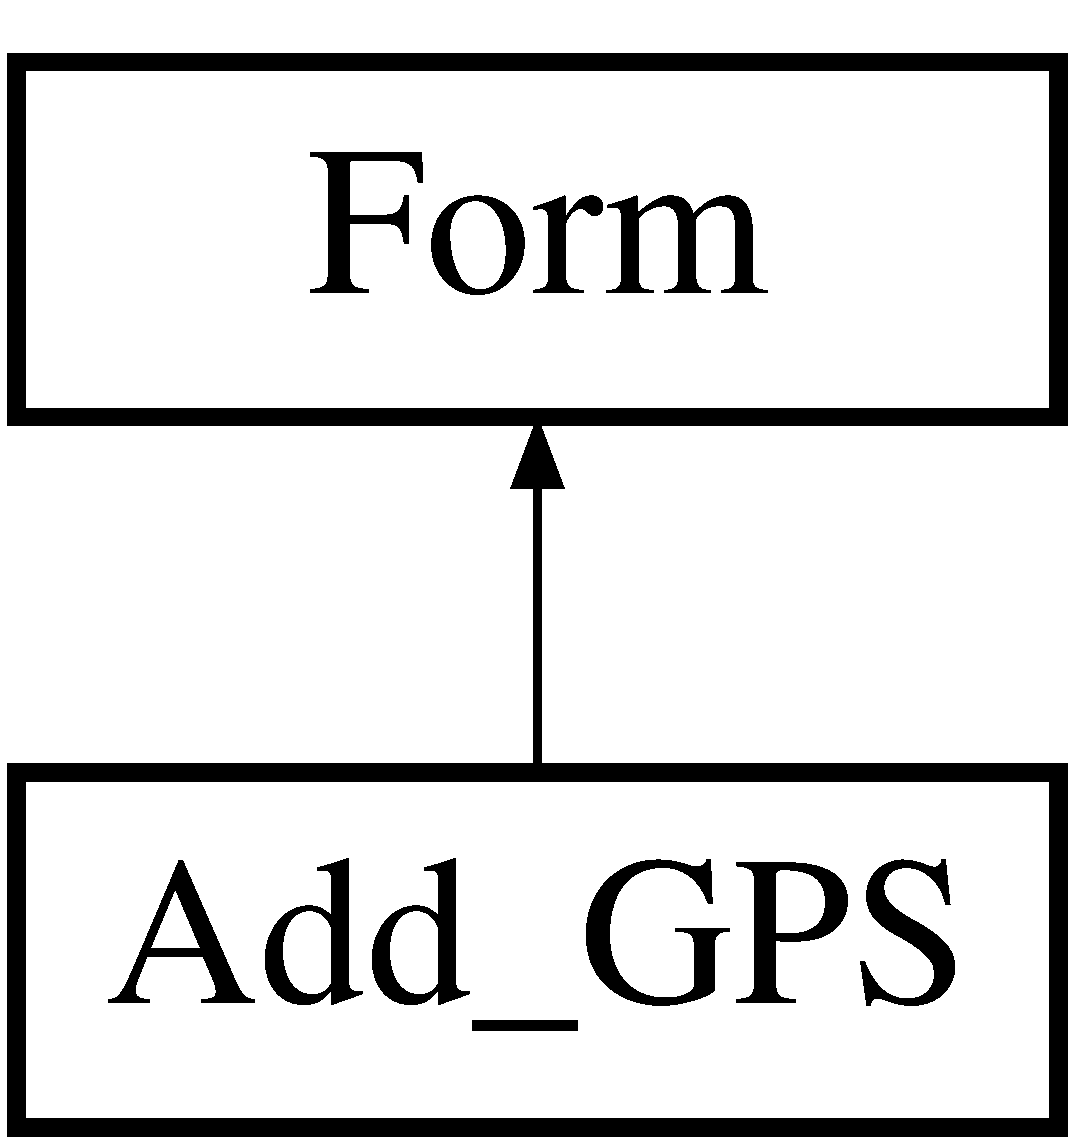
\includegraphics[height=2.000000cm]{classWildlifeTrackingApp_1_1Add__GPS}
\end{center}
\end{figure}
\subsection*{Public Member Functions}
\begin{DoxyCompactItemize}
\item 
\hyperlink{classWildlifeTrackingApp_1_1Add__GPS_a6133da1c133f9c77c5e7c7d0c68b59af}{Add\+\_\+\+G\+PS} ()
\begin{DoxyCompactList}\small\item\em Constructor for intializing log4net \end{DoxyCompactList}\end{DoxyCompactItemize}
\subsection*{Public Attributes}
\begin{DoxyCompactItemize}
\item 
string \hyperlink{classWildlifeTrackingApp_1_1Add__GPS_afd38ba6641283469fc9e94212467f9a2}{animal\+Name}
\item 
int \hyperlink{classWildlifeTrackingApp_1_1Add__GPS_a423f91c56dc35040d661cfbe357f7c78}{category\+Id}
\item 
string \hyperlink{classWildlifeTrackingApp_1_1Add__GPS_a1eca787c85e1bc45b49bbd281d4106fd}{category\+Name}
\item 
string \hyperlink{classWildlifeTrackingApp_1_1Add__GPS_aa73a9566135b30b8c5d94dde36ab0e32}{G\+P\+S\+Device\+Id}
\end{DoxyCompactItemize}
\subsection*{Protected Member Functions}
\begin{DoxyCompactItemize}
\item 
override void \hyperlink{classWildlifeTrackingApp_1_1Add__GPS_a849c3c7f8d08104f0cdb46bee9fe6389}{Dispose} (bool disposing)
\begin{DoxyCompactList}\small\item\em Clean up any resources being used. \end{DoxyCompactList}\end{DoxyCompactItemize}
\subsection*{Properties}
\begin{DoxyCompactItemize}
\item 
static log4net.\+I\+Log \hyperlink{classWildlifeTrackingApp_1_1Add__GPS_a5fc9abb86e6110ecd61d0a1a7d740a8a}{Log}\hspace{0.3cm}{\ttfamily  \mbox{[}get, private set\mbox{]}}
\end{DoxyCompactItemize}
\subsection*{Private Member Functions}
\begin{DoxyCompactItemize}
\item 
void \hyperlink{classWildlifeTrackingApp_1_1Add__GPS_ae56b21bee08f5cad9858a264ccc21fd5}{add\+\_\+button\+\_\+\+Click} (object sender, Event\+Args e)
\begin{DoxyCompactList}\small\item\em Event handler for add animal click. \end{DoxyCompactList}\item 
void \hyperlink{classWildlifeTrackingApp_1_1Add__GPS_ad3c947935fcd0474a45348ac3a08fac4}{add\+G\+P\+S\+\_\+\+Activated} (object sender, Event\+Args e)
\begin{DoxyCompactList}\small\item\em Event handler for activation of form.\+It reloads the datagrid view datasource. \end{DoxyCompactList}\item 
void \hyperlink{classWildlifeTrackingApp_1_1Add__GPS_a6405d5db675d5338663195a4d12b4c9f}{Initialize\+Component} ()
\begin{DoxyCompactList}\small\item\em Required method for Designer support -\/ do not modify the contents of this method with the code editor. \end{DoxyCompactList}\end{DoxyCompactItemize}
\subsection*{Private Attributes}
\begin{DoxyCompactItemize}
\item 
System.\+Windows.\+Forms.\+Text\+Box \hyperlink{classWildlifeTrackingApp_1_1Add__GPS_a7fe95f974f803674d4c000c9f58a9e0a}{animal\+Name\+\_\+text}
\item 
System.\+Windows.\+Forms.\+Combo\+Box \hyperlink{classWildlifeTrackingApp_1_1Add__GPS_a8b1f399ade6c575e8562bc7d574d60d5}{category\+\_\+combo\+Box}
\item 
System.\+Windows.\+Forms.\+Label \hyperlink{classWildlifeTrackingApp_1_1Add__GPS_a793869e47486b75741e1fb09829f5bc7}{category\+\_\+label}
\item 
System.\+Component\+Model.\+I\+Container \hyperlink{classWildlifeTrackingApp_1_1Add__GPS_a02595f1c09713bb71dcb2fbbfc7ffa4b}{components} = null
\begin{DoxyCompactList}\small\item\em Required designer variable. \end{DoxyCompactList}\item 
System.\+Windows.\+Forms.\+Text\+Box \hyperlink{classWildlifeTrackingApp_1_1Add__GPS_a36c825f818fa9507eea338e176dcf4b3}{gps\+Device\+Id\+\_\+\+Text}
\item 
System.\+Windows.\+Forms.\+Label \hyperlink{classWildlifeTrackingApp_1_1Add__GPS_ad153415feb3be8aba8ed0e222b9a1e32}{gps\+Id\+\_\+label}
\item 
System.\+Windows.\+Forms.\+Label \hyperlink{classWildlifeTrackingApp_1_1Add__GPS_af6ba70393d92ce2a983bf47ab956b019}{name\+\_\+label}
\item 
System.\+Windows.\+Forms.\+Button \hyperlink{classWildlifeTrackingApp_1_1Add__GPS_a6c7fe113bfa091362451d2814c3c108a}{submit\+\_\+button}
\end{DoxyCompactItemize}
\subsection*{Static Private Attributes}
\begin{DoxyCompactItemize}
\item 
static readonly log4net.\+I\+Log \hyperlink{classWildlifeTrackingApp_1_1Add__GPS_ae6c6142b8525b2f4ac6ee6e003b3106f}{log}
\end{DoxyCompactItemize}


\subsection{Detailed Description}
Form class that accepts data about new animal to be added. 



\subsection{Constructor \& Destructor Documentation}
\mbox{\Hypertarget{classWildlifeTrackingApp_1_1Add__GPS_a6133da1c133f9c77c5e7c7d0c68b59af}\label{classWildlifeTrackingApp_1_1Add__GPS_a6133da1c133f9c77c5e7c7d0c68b59af}} 
\index{Wildlife\+Tracking\+App\+::\+Add\+\_\+\+G\+PS@{Wildlife\+Tracking\+App\+::\+Add\+\_\+\+G\+PS}!Add\+\_\+\+G\+PS@{Add\+\_\+\+G\+PS}}
\index{Add\+\_\+\+G\+PS@{Add\+\_\+\+G\+PS}!Wildlife\+Tracking\+App\+::\+Add\+\_\+\+G\+PS@{Wildlife\+Tracking\+App\+::\+Add\+\_\+\+G\+PS}}
\subsubsection{\texorpdfstring{Add\+\_\+\+G\+P\+S()}{Add\_GPS()}}
{\footnotesize\ttfamily \hyperlink{classWildlifeTrackingApp_1_1Add__GPS}{Add\+\_\+\+G\+PS} (\begin{DoxyParamCaption}{ }\end{DoxyParamCaption})\hspace{0.3cm}{\ttfamily [inline]}}



Constructor for intializing log4net 



\subsection{Member Function Documentation}
\mbox{\Hypertarget{classWildlifeTrackingApp_1_1Add__GPS_ae56b21bee08f5cad9858a264ccc21fd5}\label{classWildlifeTrackingApp_1_1Add__GPS_ae56b21bee08f5cad9858a264ccc21fd5}} 
\index{Wildlife\+Tracking\+App\+::\+Add\+\_\+\+G\+PS@{Wildlife\+Tracking\+App\+::\+Add\+\_\+\+G\+PS}!add\+\_\+button\+\_\+\+Click@{add\+\_\+button\+\_\+\+Click}}
\index{add\+\_\+button\+\_\+\+Click@{add\+\_\+button\+\_\+\+Click}!Wildlife\+Tracking\+App\+::\+Add\+\_\+\+G\+PS@{Wildlife\+Tracking\+App\+::\+Add\+\_\+\+G\+PS}}
\subsubsection{\texorpdfstring{add\+\_\+button\+\_\+\+Click()}{add\_button\_Click()}}
{\footnotesize\ttfamily void add\+\_\+button\+\_\+\+Click (\begin{DoxyParamCaption}\item[{object}]{sender,  }\item[{Event\+Args}]{e }\end{DoxyParamCaption})\hspace{0.3cm}{\ttfamily [inline]}, {\ttfamily [private]}}



Event handler for add animal click. 


\begin{DoxyParams}{Parameters}
{\em sender} & Sender object\\
\hline
{\em e} & Event argument\\
\hline
\end{DoxyParams}
\mbox{\Hypertarget{classWildlifeTrackingApp_1_1Add__GPS_ad3c947935fcd0474a45348ac3a08fac4}\label{classWildlifeTrackingApp_1_1Add__GPS_ad3c947935fcd0474a45348ac3a08fac4}} 
\index{Wildlife\+Tracking\+App\+::\+Add\+\_\+\+G\+PS@{Wildlife\+Tracking\+App\+::\+Add\+\_\+\+G\+PS}!add\+G\+P\+S\+\_\+\+Activated@{add\+G\+P\+S\+\_\+\+Activated}}
\index{add\+G\+P\+S\+\_\+\+Activated@{add\+G\+P\+S\+\_\+\+Activated}!Wildlife\+Tracking\+App\+::\+Add\+\_\+\+G\+PS@{Wildlife\+Tracking\+App\+::\+Add\+\_\+\+G\+PS}}
\subsubsection{\texorpdfstring{add\+G\+P\+S\+\_\+\+Activated()}{addGPS\_Activated()}}
{\footnotesize\ttfamily void add\+G\+P\+S\+\_\+\+Activated (\begin{DoxyParamCaption}\item[{object}]{sender,  }\item[{Event\+Args}]{e }\end{DoxyParamCaption})\hspace{0.3cm}{\ttfamily [inline]}, {\ttfamily [private]}}



Event handler for activation of form.\+It reloads the datagrid view datasource. 


\begin{DoxyParams}{Parameters}
{\em sender} & Sender object\\
\hline
{\em e} & Event argument\\
\hline
\end{DoxyParams}
\mbox{\Hypertarget{classWildlifeTrackingApp_1_1Add__GPS_a849c3c7f8d08104f0cdb46bee9fe6389}\label{classWildlifeTrackingApp_1_1Add__GPS_a849c3c7f8d08104f0cdb46bee9fe6389}} 
\index{Wildlife\+Tracking\+App\+::\+Add\+\_\+\+G\+PS@{Wildlife\+Tracking\+App\+::\+Add\+\_\+\+G\+PS}!Dispose@{Dispose}}
\index{Dispose@{Dispose}!Wildlife\+Tracking\+App\+::\+Add\+\_\+\+G\+PS@{Wildlife\+Tracking\+App\+::\+Add\+\_\+\+G\+PS}}
\subsubsection{\texorpdfstring{Dispose()}{Dispose()}}
{\footnotesize\ttfamily override void Dispose (\begin{DoxyParamCaption}\item[{bool}]{disposing }\end{DoxyParamCaption})\hspace{0.3cm}{\ttfamily [inline]}, {\ttfamily [protected]}}



Clean up any resources being used. 


\begin{DoxyParams}{Parameters}
{\em disposing} & true if managed resources should be disposed; otherwise, false.\\
\hline
\end{DoxyParams}
\mbox{\Hypertarget{classWildlifeTrackingApp_1_1Add__GPS_a6405d5db675d5338663195a4d12b4c9f}\label{classWildlifeTrackingApp_1_1Add__GPS_a6405d5db675d5338663195a4d12b4c9f}} 
\index{Wildlife\+Tracking\+App\+::\+Add\+\_\+\+G\+PS@{Wildlife\+Tracking\+App\+::\+Add\+\_\+\+G\+PS}!Initialize\+Component@{Initialize\+Component}}
\index{Initialize\+Component@{Initialize\+Component}!Wildlife\+Tracking\+App\+::\+Add\+\_\+\+G\+PS@{Wildlife\+Tracking\+App\+::\+Add\+\_\+\+G\+PS}}
\subsubsection{\texorpdfstring{Initialize\+Component()}{InitializeComponent()}}
{\footnotesize\ttfamily void Initialize\+Component (\begin{DoxyParamCaption}{ }\end{DoxyParamCaption})\hspace{0.3cm}{\ttfamily [inline]}, {\ttfamily [private]}}



Required method for Designer support -\/ do not modify the contents of this method with the code editor. 



\subsection{Member Data Documentation}
\mbox{\Hypertarget{classWildlifeTrackingApp_1_1Add__GPS_afd38ba6641283469fc9e94212467f9a2}\label{classWildlifeTrackingApp_1_1Add__GPS_afd38ba6641283469fc9e94212467f9a2}} 
\index{Wildlife\+Tracking\+App\+::\+Add\+\_\+\+G\+PS@{Wildlife\+Tracking\+App\+::\+Add\+\_\+\+G\+PS}!animal\+Name@{animal\+Name}}
\index{animal\+Name@{animal\+Name}!Wildlife\+Tracking\+App\+::\+Add\+\_\+\+G\+PS@{Wildlife\+Tracking\+App\+::\+Add\+\_\+\+G\+PS}}
\subsubsection{\texorpdfstring{animal\+Name}{animalName}}
{\footnotesize\ttfamily string animal\+Name}

\mbox{\Hypertarget{classWildlifeTrackingApp_1_1Add__GPS_a7fe95f974f803674d4c000c9f58a9e0a}\label{classWildlifeTrackingApp_1_1Add__GPS_a7fe95f974f803674d4c000c9f58a9e0a}} 
\index{Wildlife\+Tracking\+App\+::\+Add\+\_\+\+G\+PS@{Wildlife\+Tracking\+App\+::\+Add\+\_\+\+G\+PS}!animal\+Name\+\_\+text@{animal\+Name\+\_\+text}}
\index{animal\+Name\+\_\+text@{animal\+Name\+\_\+text}!Wildlife\+Tracking\+App\+::\+Add\+\_\+\+G\+PS@{Wildlife\+Tracking\+App\+::\+Add\+\_\+\+G\+PS}}
\subsubsection{\texorpdfstring{animal\+Name\+\_\+text}{animalName\_text}}
{\footnotesize\ttfamily System.\+Windows.\+Forms.\+Text\+Box animal\+Name\+\_\+text\hspace{0.3cm}{\ttfamily [private]}}

\mbox{\Hypertarget{classWildlifeTrackingApp_1_1Add__GPS_a8b1f399ade6c575e8562bc7d574d60d5}\label{classWildlifeTrackingApp_1_1Add__GPS_a8b1f399ade6c575e8562bc7d574d60d5}} 
\index{Wildlife\+Tracking\+App\+::\+Add\+\_\+\+G\+PS@{Wildlife\+Tracking\+App\+::\+Add\+\_\+\+G\+PS}!category\+\_\+combo\+Box@{category\+\_\+combo\+Box}}
\index{category\+\_\+combo\+Box@{category\+\_\+combo\+Box}!Wildlife\+Tracking\+App\+::\+Add\+\_\+\+G\+PS@{Wildlife\+Tracking\+App\+::\+Add\+\_\+\+G\+PS}}
\subsubsection{\texorpdfstring{category\+\_\+combo\+Box}{category\_comboBox}}
{\footnotesize\ttfamily System.\+Windows.\+Forms.\+Combo\+Box category\+\_\+combo\+Box\hspace{0.3cm}{\ttfamily [private]}}

\mbox{\Hypertarget{classWildlifeTrackingApp_1_1Add__GPS_a793869e47486b75741e1fb09829f5bc7}\label{classWildlifeTrackingApp_1_1Add__GPS_a793869e47486b75741e1fb09829f5bc7}} 
\index{Wildlife\+Tracking\+App\+::\+Add\+\_\+\+G\+PS@{Wildlife\+Tracking\+App\+::\+Add\+\_\+\+G\+PS}!category\+\_\+label@{category\+\_\+label}}
\index{category\+\_\+label@{category\+\_\+label}!Wildlife\+Tracking\+App\+::\+Add\+\_\+\+G\+PS@{Wildlife\+Tracking\+App\+::\+Add\+\_\+\+G\+PS}}
\subsubsection{\texorpdfstring{category\+\_\+label}{category\_label}}
{\footnotesize\ttfamily System.\+Windows.\+Forms.\+Label category\+\_\+label\hspace{0.3cm}{\ttfamily [private]}}

\mbox{\Hypertarget{classWildlifeTrackingApp_1_1Add__GPS_a423f91c56dc35040d661cfbe357f7c78}\label{classWildlifeTrackingApp_1_1Add__GPS_a423f91c56dc35040d661cfbe357f7c78}} 
\index{Wildlife\+Tracking\+App\+::\+Add\+\_\+\+G\+PS@{Wildlife\+Tracking\+App\+::\+Add\+\_\+\+G\+PS}!category\+Id@{category\+Id}}
\index{category\+Id@{category\+Id}!Wildlife\+Tracking\+App\+::\+Add\+\_\+\+G\+PS@{Wildlife\+Tracking\+App\+::\+Add\+\_\+\+G\+PS}}
\subsubsection{\texorpdfstring{category\+Id}{categoryId}}
{\footnotesize\ttfamily int category\+Id}

\mbox{\Hypertarget{classWildlifeTrackingApp_1_1Add__GPS_a1eca787c85e1bc45b49bbd281d4106fd}\label{classWildlifeTrackingApp_1_1Add__GPS_a1eca787c85e1bc45b49bbd281d4106fd}} 
\index{Wildlife\+Tracking\+App\+::\+Add\+\_\+\+G\+PS@{Wildlife\+Tracking\+App\+::\+Add\+\_\+\+G\+PS}!category\+Name@{category\+Name}}
\index{category\+Name@{category\+Name}!Wildlife\+Tracking\+App\+::\+Add\+\_\+\+G\+PS@{Wildlife\+Tracking\+App\+::\+Add\+\_\+\+G\+PS}}
\subsubsection{\texorpdfstring{category\+Name}{categoryName}}
{\footnotesize\ttfamily string category\+Name}

\mbox{\Hypertarget{classWildlifeTrackingApp_1_1Add__GPS_a02595f1c09713bb71dcb2fbbfc7ffa4b}\label{classWildlifeTrackingApp_1_1Add__GPS_a02595f1c09713bb71dcb2fbbfc7ffa4b}} 
\index{Wildlife\+Tracking\+App\+::\+Add\+\_\+\+G\+PS@{Wildlife\+Tracking\+App\+::\+Add\+\_\+\+G\+PS}!components@{components}}
\index{components@{components}!Wildlife\+Tracking\+App\+::\+Add\+\_\+\+G\+PS@{Wildlife\+Tracking\+App\+::\+Add\+\_\+\+G\+PS}}
\subsubsection{\texorpdfstring{components}{components}}
{\footnotesize\ttfamily System.\+Component\+Model.\+I\+Container components = null\hspace{0.3cm}{\ttfamily [private]}}



Required designer variable. 

\mbox{\Hypertarget{classWildlifeTrackingApp_1_1Add__GPS_aa73a9566135b30b8c5d94dde36ab0e32}\label{classWildlifeTrackingApp_1_1Add__GPS_aa73a9566135b30b8c5d94dde36ab0e32}} 
\index{Wildlife\+Tracking\+App\+::\+Add\+\_\+\+G\+PS@{Wildlife\+Tracking\+App\+::\+Add\+\_\+\+G\+PS}!G\+P\+S\+Device\+Id@{G\+P\+S\+Device\+Id}}
\index{G\+P\+S\+Device\+Id@{G\+P\+S\+Device\+Id}!Wildlife\+Tracking\+App\+::\+Add\+\_\+\+G\+PS@{Wildlife\+Tracking\+App\+::\+Add\+\_\+\+G\+PS}}
\subsubsection{\texorpdfstring{G\+P\+S\+Device\+Id}{GPSDeviceId}}
{\footnotesize\ttfamily string G\+P\+S\+Device\+Id}

\mbox{\Hypertarget{classWildlifeTrackingApp_1_1Add__GPS_a36c825f818fa9507eea338e176dcf4b3}\label{classWildlifeTrackingApp_1_1Add__GPS_a36c825f818fa9507eea338e176dcf4b3}} 
\index{Wildlife\+Tracking\+App\+::\+Add\+\_\+\+G\+PS@{Wildlife\+Tracking\+App\+::\+Add\+\_\+\+G\+PS}!gps\+Device\+Id\+\_\+\+Text@{gps\+Device\+Id\+\_\+\+Text}}
\index{gps\+Device\+Id\+\_\+\+Text@{gps\+Device\+Id\+\_\+\+Text}!Wildlife\+Tracking\+App\+::\+Add\+\_\+\+G\+PS@{Wildlife\+Tracking\+App\+::\+Add\+\_\+\+G\+PS}}
\subsubsection{\texorpdfstring{gps\+Device\+Id\+\_\+\+Text}{gpsDeviceId\_Text}}
{\footnotesize\ttfamily System.\+Windows.\+Forms.\+Text\+Box gps\+Device\+Id\+\_\+\+Text\hspace{0.3cm}{\ttfamily [private]}}

\mbox{\Hypertarget{classWildlifeTrackingApp_1_1Add__GPS_ad153415feb3be8aba8ed0e222b9a1e32}\label{classWildlifeTrackingApp_1_1Add__GPS_ad153415feb3be8aba8ed0e222b9a1e32}} 
\index{Wildlife\+Tracking\+App\+::\+Add\+\_\+\+G\+PS@{Wildlife\+Tracking\+App\+::\+Add\+\_\+\+G\+PS}!gps\+Id\+\_\+label@{gps\+Id\+\_\+label}}
\index{gps\+Id\+\_\+label@{gps\+Id\+\_\+label}!Wildlife\+Tracking\+App\+::\+Add\+\_\+\+G\+PS@{Wildlife\+Tracking\+App\+::\+Add\+\_\+\+G\+PS}}
\subsubsection{\texorpdfstring{gps\+Id\+\_\+label}{gpsId\_label}}
{\footnotesize\ttfamily System.\+Windows.\+Forms.\+Label gps\+Id\+\_\+label\hspace{0.3cm}{\ttfamily [private]}}

\mbox{\Hypertarget{classWildlifeTrackingApp_1_1Add__GPS_ae6c6142b8525b2f4ac6ee6e003b3106f}\label{classWildlifeTrackingApp_1_1Add__GPS_ae6c6142b8525b2f4ac6ee6e003b3106f}} 
\index{Wildlife\+Tracking\+App\+::\+Add\+\_\+\+G\+PS@{Wildlife\+Tracking\+App\+::\+Add\+\_\+\+G\+PS}!log@{log}}
\index{log@{log}!Wildlife\+Tracking\+App\+::\+Add\+\_\+\+G\+PS@{Wildlife\+Tracking\+App\+::\+Add\+\_\+\+G\+PS}}
\subsubsection{\texorpdfstring{log}{log}}
{\footnotesize\ttfamily readonly log4net.\+I\+Log log\hspace{0.3cm}{\ttfamily [static]}, {\ttfamily [private]}}

{\bfseries Initial value\+:}
\begin{DoxyCode}
= log4net.LogManager.GetLogger
        (\hyperlink{namespaceSystem}{System}.Reflection.MethodBase.GetCurrentMethod().DeclaringType)
\end{DoxyCode}
\mbox{\Hypertarget{classWildlifeTrackingApp_1_1Add__GPS_af6ba70393d92ce2a983bf47ab956b019}\label{classWildlifeTrackingApp_1_1Add__GPS_af6ba70393d92ce2a983bf47ab956b019}} 
\index{Wildlife\+Tracking\+App\+::\+Add\+\_\+\+G\+PS@{Wildlife\+Tracking\+App\+::\+Add\+\_\+\+G\+PS}!name\+\_\+label@{name\+\_\+label}}
\index{name\+\_\+label@{name\+\_\+label}!Wildlife\+Tracking\+App\+::\+Add\+\_\+\+G\+PS@{Wildlife\+Tracking\+App\+::\+Add\+\_\+\+G\+PS}}
\subsubsection{\texorpdfstring{name\+\_\+label}{name\_label}}
{\footnotesize\ttfamily System.\+Windows.\+Forms.\+Label name\+\_\+label\hspace{0.3cm}{\ttfamily [private]}}

\mbox{\Hypertarget{classWildlifeTrackingApp_1_1Add__GPS_a6c7fe113bfa091362451d2814c3c108a}\label{classWildlifeTrackingApp_1_1Add__GPS_a6c7fe113bfa091362451d2814c3c108a}} 
\index{Wildlife\+Tracking\+App\+::\+Add\+\_\+\+G\+PS@{Wildlife\+Tracking\+App\+::\+Add\+\_\+\+G\+PS}!submit\+\_\+button@{submit\+\_\+button}}
\index{submit\+\_\+button@{submit\+\_\+button}!Wildlife\+Tracking\+App\+::\+Add\+\_\+\+G\+PS@{Wildlife\+Tracking\+App\+::\+Add\+\_\+\+G\+PS}}
\subsubsection{\texorpdfstring{submit\+\_\+button}{submit\_button}}
{\footnotesize\ttfamily System.\+Windows.\+Forms.\+Button submit\+\_\+button\hspace{0.3cm}{\ttfamily [private]}}



\subsection{Property Documentation}
\mbox{\Hypertarget{classWildlifeTrackingApp_1_1Add__GPS_a5fc9abb86e6110ecd61d0a1a7d740a8a}\label{classWildlifeTrackingApp_1_1Add__GPS_a5fc9abb86e6110ecd61d0a1a7d740a8a}} 
\index{Wildlife\+Tracking\+App\+::\+Add\+\_\+\+G\+PS@{Wildlife\+Tracking\+App\+::\+Add\+\_\+\+G\+PS}!Log@{Log}}
\index{Log@{Log}!Wildlife\+Tracking\+App\+::\+Add\+\_\+\+G\+PS@{Wildlife\+Tracking\+App\+::\+Add\+\_\+\+G\+PS}}
\subsubsection{\texorpdfstring{Log}{Log}}
{\footnotesize\ttfamily log4net.\+I\+Log Log\hspace{0.3cm}{\ttfamily [static]}, {\ttfamily [get]}, {\ttfamily [private set]}}



The documentation for this class was generated from the following files\+:\begin{DoxyCompactItemize}
\item 
View/\hyperlink{Add_01GPS_8cs}{Add G\+P\+S.\+cs}\item 
View/\hyperlink{Add_01GPS_8Designer_8cs}{Add G\+P\+S.\+Designer.\+cs}\end{DoxyCompactItemize}

\hypertarget{classWildlifeTrackingApp_1_1AddCategory}{}\section{Add\+Category}
\label{classWildlifeTrackingApp_1_1AddCategory}\index{Add\+Category@{Add\+Category}}


Form class that accepts datas of new category to be added.  


Inheritance diagram for Add\+Category\+:\begin{figure}[H]
\begin{center}
\leavevmode
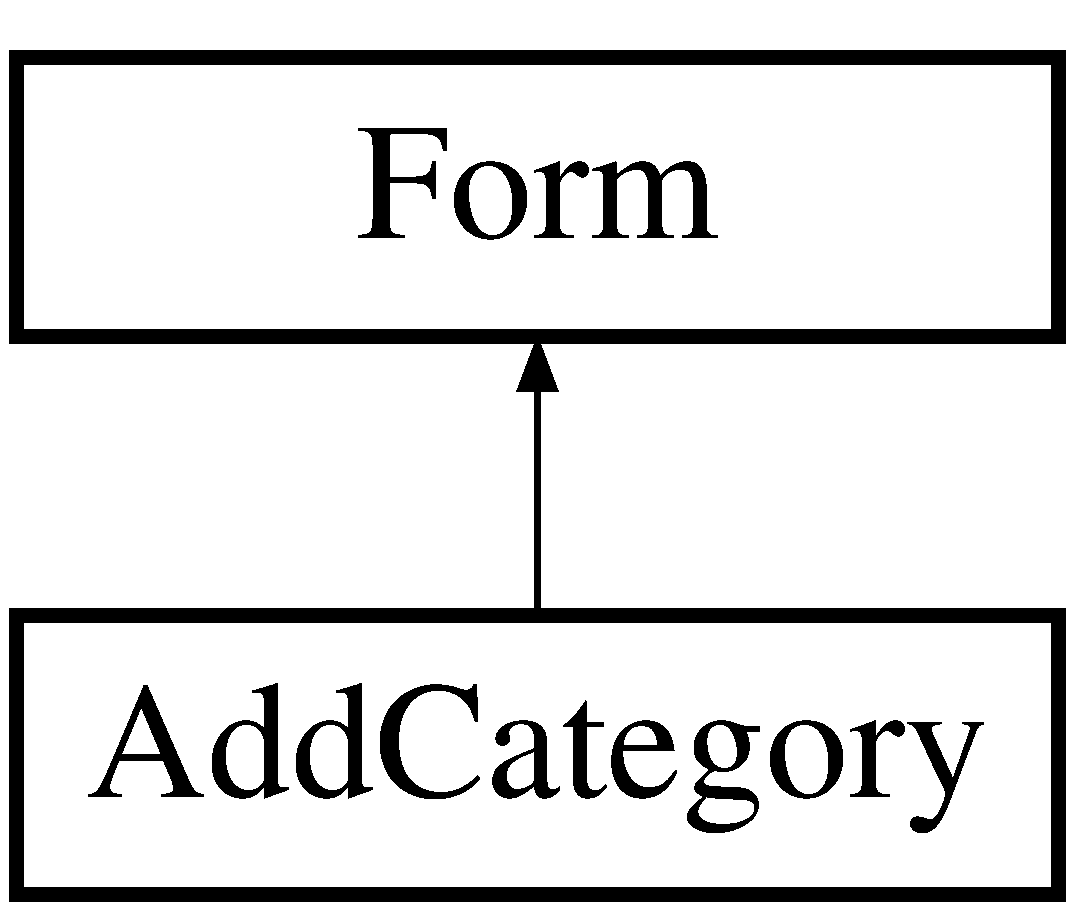
\includegraphics[height=2.000000cm]{classWildlifeTrackingApp_1_1AddCategory}
\end{center}
\end{figure}
\subsection*{Public Member Functions}
\begin{DoxyCompactItemize}
\item 
\hyperlink{classWildlifeTrackingApp_1_1AddCategory_af7eaf46f7b2758e1c6af7c0290322940}{Add\+Category} ()
\end{DoxyCompactItemize}
\subsection*{Public Attributes}
\begin{DoxyCompactItemize}
\item 
string \hyperlink{classWildlifeTrackingApp_1_1AddCategory_a1eca787c85e1bc45b49bbd281d4106fd}{category\+Name}
\item 
string \hyperlink{classWildlifeTrackingApp_1_1AddCategory_acccfd1715ce280fb9d9171cd4dfd387a}{color\+Hex\+Code}
\item 
string \hyperlink{classWildlifeTrackingApp_1_1AddCategory_ae96d6391386605736c8c89605e7258b6}{color\+Hex\+Value}
\item 
string \hyperlink{classWildlifeTrackingApp_1_1AddCategory_a23af17c78302b71c14ef38ea40b8d1d7}{description}
\end{DoxyCompactItemize}
\subsection*{Protected Member Functions}
\begin{DoxyCompactItemize}
\item 
override void \hyperlink{classWildlifeTrackingApp_1_1AddCategory_a849c3c7f8d08104f0cdb46bee9fe6389}{Dispose} (bool disposing)
\begin{DoxyCompactList}\small\item\em Clean up any resources being used. \end{DoxyCompactList}\end{DoxyCompactItemize}
\subsection*{Properties}
\begin{DoxyCompactItemize}
\item 
static log4net.\+I\+Log \hyperlink{classWildlifeTrackingApp_1_1AddCategory_a5fc9abb86e6110ecd61d0a1a7d740a8a}{Log}\hspace{0.3cm}{\ttfamily  \mbox{[}get, private set\mbox{]}}
\end{DoxyCompactItemize}
\subsection*{Private Member Functions}
\begin{DoxyCompactItemize}
\item 
void \hyperlink{classWildlifeTrackingApp_1_1AddCategory_a6405d5db675d5338663195a4d12b4c9f}{Initialize\+Component} ()
\begin{DoxyCompactList}\small\item\em Required method for Designer support -\/ do not modify the contents of this method with the code editor. \end{DoxyCompactList}\item 
void \hyperlink{classWildlifeTrackingApp_1_1AddCategory_a98c6d7308f3d8ce093b205cec7b9422a}{select\+Color\+\_\+button\+\_\+\+Click} (object sender, Event\+Args e)
\begin{DoxyCompactList}\small\item\em Event handler for select color button click. Color dialog box will pop up. \end{DoxyCompactList}\item 
void \hyperlink{classWildlifeTrackingApp_1_1AddCategory_a4a8fd9eeb145ce142cc04944541ff56a}{submit\+\_\+button\+\_\+\+Click} (object sender, Event\+Args e)
\begin{DoxyCompactList}\small\item\em Event handler for submit button click.\+It accepts input fields and store in client. \end{DoxyCompactList}\end{DoxyCompactItemize}
\subsection*{Private Attributes}
\begin{DoxyCompactItemize}
\item 
System.\+Windows.\+Forms.\+Text\+Box \hyperlink{classWildlifeTrackingApp_1_1AddCategory_af32de17dc2e977c753051e4fda44cba1}{color\+\_\+text\+Box}
\item 
System.\+Windows.\+Forms.\+Color\+Dialog \hyperlink{classWildlifeTrackingApp_1_1AddCategory_af5ea1053a29b769cb6970f4f987b6fc1}{color\+Dialog}
\item 
System.\+Component\+Model.\+I\+Container \hyperlink{classWildlifeTrackingApp_1_1AddCategory_a02595f1c09713bb71dcb2fbbfc7ffa4b}{components} = null
\begin{DoxyCompactList}\small\item\em Required designer variable. \end{DoxyCompactList}\item 
System.\+Windows.\+Forms.\+Label \hyperlink{classWildlifeTrackingApp_1_1AddCategory_a5a1799944a6da4432adf81c9403918ed}{description\+\_\+label}
\item 
System.\+Windows.\+Forms.\+Rich\+Text\+Box \hyperlink{classWildlifeTrackingApp_1_1AddCategory_a0760a97883bbcc1aa4ef20db02c81505}{description\+\_\+rich\+Text\+Box}
\item 
System.\+Windows.\+Forms.\+Label \hyperlink{classWildlifeTrackingApp_1_1AddCategory_aa4d0e09997f0ef76f00a520b0b8228c2}{mandatory\+\_\+label}
\item 
System.\+Windows.\+Forms.\+Label \hyperlink{classWildlifeTrackingApp_1_1AddCategory_a8d0d54f782d0abb2f21bab81d8c21dd9}{mandatory\+\_\+label1}
\item 
System.\+Windows.\+Forms.\+Label \hyperlink{classWildlifeTrackingApp_1_1AddCategory_af6ba70393d92ce2a983bf47ab956b019}{name\+\_\+label}
\item 
System.\+Windows.\+Forms.\+Text\+Box \hyperlink{classWildlifeTrackingApp_1_1AddCategory_aa359962ce074ab9473880842aecc6353}{name\+\_\+text\+Box}
\item 
System.\+Windows.\+Forms.\+Button \hyperlink{classWildlifeTrackingApp_1_1AddCategory_ab9917c7bafb007d23c574c8d7d1049ac}{select\+Color\+\_\+button}
\item 
System.\+Windows.\+Forms.\+Button \hyperlink{classWildlifeTrackingApp_1_1AddCategory_a6c7fe113bfa091362451d2814c3c108a}{submit\+\_\+button}
\end{DoxyCompactItemize}
\subsection*{Static Private Attributes}
\begin{DoxyCompactItemize}
\item 
static readonly log4net.\+I\+Log \hyperlink{classWildlifeTrackingApp_1_1AddCategory_ae6c6142b8525b2f4ac6ee6e003b3106f}{log}
\end{DoxyCompactItemize}


\subsection{Detailed Description}
Form class that accepts datas of new category to be added. 



\subsection{Constructor \& Destructor Documentation}
\mbox{\Hypertarget{classWildlifeTrackingApp_1_1AddCategory_af7eaf46f7b2758e1c6af7c0290322940}\label{classWildlifeTrackingApp_1_1AddCategory_af7eaf46f7b2758e1c6af7c0290322940}} 
\index{Wildlife\+Tracking\+App\+::\+Add\+Category@{Wildlife\+Tracking\+App\+::\+Add\+Category}!Add\+Category@{Add\+Category}}
\index{Add\+Category@{Add\+Category}!Wildlife\+Tracking\+App\+::\+Add\+Category@{Wildlife\+Tracking\+App\+::\+Add\+Category}}
\subsubsection{\texorpdfstring{Add\+Category()}{AddCategory()}}
{\footnotesize\ttfamily \hyperlink{classWildlifeTrackingApp_1_1AddCategory}{Add\+Category} (\begin{DoxyParamCaption}{ }\end{DoxyParamCaption})\hspace{0.3cm}{\ttfamily [inline]}}



\subsection{Member Function Documentation}
\mbox{\Hypertarget{classWildlifeTrackingApp_1_1AddCategory_a849c3c7f8d08104f0cdb46bee9fe6389}\label{classWildlifeTrackingApp_1_1AddCategory_a849c3c7f8d08104f0cdb46bee9fe6389}} 
\index{Wildlife\+Tracking\+App\+::\+Add\+Category@{Wildlife\+Tracking\+App\+::\+Add\+Category}!Dispose@{Dispose}}
\index{Dispose@{Dispose}!Wildlife\+Tracking\+App\+::\+Add\+Category@{Wildlife\+Tracking\+App\+::\+Add\+Category}}
\subsubsection{\texorpdfstring{Dispose()}{Dispose()}}
{\footnotesize\ttfamily override void Dispose (\begin{DoxyParamCaption}\item[{bool}]{disposing }\end{DoxyParamCaption})\hspace{0.3cm}{\ttfamily [inline]}, {\ttfamily [protected]}}



Clean up any resources being used. 


\begin{DoxyParams}{Parameters}
{\em disposing} & true if managed resources should be disposed; otherwise, false.\\
\hline
\end{DoxyParams}
\mbox{\Hypertarget{classWildlifeTrackingApp_1_1AddCategory_a6405d5db675d5338663195a4d12b4c9f}\label{classWildlifeTrackingApp_1_1AddCategory_a6405d5db675d5338663195a4d12b4c9f}} 
\index{Wildlife\+Tracking\+App\+::\+Add\+Category@{Wildlife\+Tracking\+App\+::\+Add\+Category}!Initialize\+Component@{Initialize\+Component}}
\index{Initialize\+Component@{Initialize\+Component}!Wildlife\+Tracking\+App\+::\+Add\+Category@{Wildlife\+Tracking\+App\+::\+Add\+Category}}
\subsubsection{\texorpdfstring{Initialize\+Component()}{InitializeComponent()}}
{\footnotesize\ttfamily void Initialize\+Component (\begin{DoxyParamCaption}{ }\end{DoxyParamCaption})\hspace{0.3cm}{\ttfamily [inline]}, {\ttfamily [private]}}



Required method for Designer support -\/ do not modify the contents of this method with the code editor. 

\mbox{\Hypertarget{classWildlifeTrackingApp_1_1AddCategory_a98c6d7308f3d8ce093b205cec7b9422a}\label{classWildlifeTrackingApp_1_1AddCategory_a98c6d7308f3d8ce093b205cec7b9422a}} 
\index{Wildlife\+Tracking\+App\+::\+Add\+Category@{Wildlife\+Tracking\+App\+::\+Add\+Category}!select\+Color\+\_\+button\+\_\+\+Click@{select\+Color\+\_\+button\+\_\+\+Click}}
\index{select\+Color\+\_\+button\+\_\+\+Click@{select\+Color\+\_\+button\+\_\+\+Click}!Wildlife\+Tracking\+App\+::\+Add\+Category@{Wildlife\+Tracking\+App\+::\+Add\+Category}}
\subsubsection{\texorpdfstring{select\+Color\+\_\+button\+\_\+\+Click()}{selectColor\_button\_Click()}}
{\footnotesize\ttfamily void select\+Color\+\_\+button\+\_\+\+Click (\begin{DoxyParamCaption}\item[{object}]{sender,  }\item[{Event\+Args}]{e }\end{DoxyParamCaption})\hspace{0.3cm}{\ttfamily [inline]}, {\ttfamily [private]}}



Event handler for select color button click. Color dialog box will pop up. 


\begin{DoxyParams}{Parameters}
{\em sender} & Sender object\\
\hline
{\em e} & Event argument\\
\hline
\end{DoxyParams}
\mbox{\Hypertarget{classWildlifeTrackingApp_1_1AddCategory_a4a8fd9eeb145ce142cc04944541ff56a}\label{classWildlifeTrackingApp_1_1AddCategory_a4a8fd9eeb145ce142cc04944541ff56a}} 
\index{Wildlife\+Tracking\+App\+::\+Add\+Category@{Wildlife\+Tracking\+App\+::\+Add\+Category}!submit\+\_\+button\+\_\+\+Click@{submit\+\_\+button\+\_\+\+Click}}
\index{submit\+\_\+button\+\_\+\+Click@{submit\+\_\+button\+\_\+\+Click}!Wildlife\+Tracking\+App\+::\+Add\+Category@{Wildlife\+Tracking\+App\+::\+Add\+Category}}
\subsubsection{\texorpdfstring{submit\+\_\+button\+\_\+\+Click()}{submit\_button\_Click()}}
{\footnotesize\ttfamily void submit\+\_\+button\+\_\+\+Click (\begin{DoxyParamCaption}\item[{object}]{sender,  }\item[{Event\+Args}]{e }\end{DoxyParamCaption})\hspace{0.3cm}{\ttfamily [inline]}, {\ttfamily [private]}}



Event handler for submit button click.\+It accepts input fields and store in client. 


\begin{DoxyParams}{Parameters}
{\em sender} & Sender object\\
\hline
{\em e} & Event argument\\
\hline
\end{DoxyParams}


\subsection{Member Data Documentation}
\mbox{\Hypertarget{classWildlifeTrackingApp_1_1AddCategory_a1eca787c85e1bc45b49bbd281d4106fd}\label{classWildlifeTrackingApp_1_1AddCategory_a1eca787c85e1bc45b49bbd281d4106fd}} 
\index{Wildlife\+Tracking\+App\+::\+Add\+Category@{Wildlife\+Tracking\+App\+::\+Add\+Category}!category\+Name@{category\+Name}}
\index{category\+Name@{category\+Name}!Wildlife\+Tracking\+App\+::\+Add\+Category@{Wildlife\+Tracking\+App\+::\+Add\+Category}}
\subsubsection{\texorpdfstring{category\+Name}{categoryName}}
{\footnotesize\ttfamily string category\+Name}

\mbox{\Hypertarget{classWildlifeTrackingApp_1_1AddCategory_af32de17dc2e977c753051e4fda44cba1}\label{classWildlifeTrackingApp_1_1AddCategory_af32de17dc2e977c753051e4fda44cba1}} 
\index{Wildlife\+Tracking\+App\+::\+Add\+Category@{Wildlife\+Tracking\+App\+::\+Add\+Category}!color\+\_\+text\+Box@{color\+\_\+text\+Box}}
\index{color\+\_\+text\+Box@{color\+\_\+text\+Box}!Wildlife\+Tracking\+App\+::\+Add\+Category@{Wildlife\+Tracking\+App\+::\+Add\+Category}}
\subsubsection{\texorpdfstring{color\+\_\+text\+Box}{color\_textBox}}
{\footnotesize\ttfamily System.\+Windows.\+Forms.\+Text\+Box color\+\_\+text\+Box\hspace{0.3cm}{\ttfamily [private]}}

\mbox{\Hypertarget{classWildlifeTrackingApp_1_1AddCategory_af5ea1053a29b769cb6970f4f987b6fc1}\label{classWildlifeTrackingApp_1_1AddCategory_af5ea1053a29b769cb6970f4f987b6fc1}} 
\index{Wildlife\+Tracking\+App\+::\+Add\+Category@{Wildlife\+Tracking\+App\+::\+Add\+Category}!color\+Dialog@{color\+Dialog}}
\index{color\+Dialog@{color\+Dialog}!Wildlife\+Tracking\+App\+::\+Add\+Category@{Wildlife\+Tracking\+App\+::\+Add\+Category}}
\subsubsection{\texorpdfstring{color\+Dialog}{colorDialog}}
{\footnotesize\ttfamily System.\+Windows.\+Forms.\+Color\+Dialog color\+Dialog\hspace{0.3cm}{\ttfamily [private]}}

\mbox{\Hypertarget{classWildlifeTrackingApp_1_1AddCategory_acccfd1715ce280fb9d9171cd4dfd387a}\label{classWildlifeTrackingApp_1_1AddCategory_acccfd1715ce280fb9d9171cd4dfd387a}} 
\index{Wildlife\+Tracking\+App\+::\+Add\+Category@{Wildlife\+Tracking\+App\+::\+Add\+Category}!color\+Hex\+Code@{color\+Hex\+Code}}
\index{color\+Hex\+Code@{color\+Hex\+Code}!Wildlife\+Tracking\+App\+::\+Add\+Category@{Wildlife\+Tracking\+App\+::\+Add\+Category}}
\subsubsection{\texorpdfstring{color\+Hex\+Code}{colorHexCode}}
{\footnotesize\ttfamily string color\+Hex\+Code}

\mbox{\Hypertarget{classWildlifeTrackingApp_1_1AddCategory_ae96d6391386605736c8c89605e7258b6}\label{classWildlifeTrackingApp_1_1AddCategory_ae96d6391386605736c8c89605e7258b6}} 
\index{Wildlife\+Tracking\+App\+::\+Add\+Category@{Wildlife\+Tracking\+App\+::\+Add\+Category}!color\+Hex\+Value@{color\+Hex\+Value}}
\index{color\+Hex\+Value@{color\+Hex\+Value}!Wildlife\+Tracking\+App\+::\+Add\+Category@{Wildlife\+Tracking\+App\+::\+Add\+Category}}
\subsubsection{\texorpdfstring{color\+Hex\+Value}{colorHexValue}}
{\footnotesize\ttfamily string color\+Hex\+Value}

\mbox{\Hypertarget{classWildlifeTrackingApp_1_1AddCategory_a02595f1c09713bb71dcb2fbbfc7ffa4b}\label{classWildlifeTrackingApp_1_1AddCategory_a02595f1c09713bb71dcb2fbbfc7ffa4b}} 
\index{Wildlife\+Tracking\+App\+::\+Add\+Category@{Wildlife\+Tracking\+App\+::\+Add\+Category}!components@{components}}
\index{components@{components}!Wildlife\+Tracking\+App\+::\+Add\+Category@{Wildlife\+Tracking\+App\+::\+Add\+Category}}
\subsubsection{\texorpdfstring{components}{components}}
{\footnotesize\ttfamily System.\+Component\+Model.\+I\+Container components = null\hspace{0.3cm}{\ttfamily [private]}}



Required designer variable. 

\mbox{\Hypertarget{classWildlifeTrackingApp_1_1AddCategory_a23af17c78302b71c14ef38ea40b8d1d7}\label{classWildlifeTrackingApp_1_1AddCategory_a23af17c78302b71c14ef38ea40b8d1d7}} 
\index{Wildlife\+Tracking\+App\+::\+Add\+Category@{Wildlife\+Tracking\+App\+::\+Add\+Category}!description@{description}}
\index{description@{description}!Wildlife\+Tracking\+App\+::\+Add\+Category@{Wildlife\+Tracking\+App\+::\+Add\+Category}}
\subsubsection{\texorpdfstring{description}{description}}
{\footnotesize\ttfamily string description}

\mbox{\Hypertarget{classWildlifeTrackingApp_1_1AddCategory_a5a1799944a6da4432adf81c9403918ed}\label{classWildlifeTrackingApp_1_1AddCategory_a5a1799944a6da4432adf81c9403918ed}} 
\index{Wildlife\+Tracking\+App\+::\+Add\+Category@{Wildlife\+Tracking\+App\+::\+Add\+Category}!description\+\_\+label@{description\+\_\+label}}
\index{description\+\_\+label@{description\+\_\+label}!Wildlife\+Tracking\+App\+::\+Add\+Category@{Wildlife\+Tracking\+App\+::\+Add\+Category}}
\subsubsection{\texorpdfstring{description\+\_\+label}{description\_label}}
{\footnotesize\ttfamily System.\+Windows.\+Forms.\+Label description\+\_\+label\hspace{0.3cm}{\ttfamily [private]}}

\mbox{\Hypertarget{classWildlifeTrackingApp_1_1AddCategory_a0760a97883bbcc1aa4ef20db02c81505}\label{classWildlifeTrackingApp_1_1AddCategory_a0760a97883bbcc1aa4ef20db02c81505}} 
\index{Wildlife\+Tracking\+App\+::\+Add\+Category@{Wildlife\+Tracking\+App\+::\+Add\+Category}!description\+\_\+rich\+Text\+Box@{description\+\_\+rich\+Text\+Box}}
\index{description\+\_\+rich\+Text\+Box@{description\+\_\+rich\+Text\+Box}!Wildlife\+Tracking\+App\+::\+Add\+Category@{Wildlife\+Tracking\+App\+::\+Add\+Category}}
\subsubsection{\texorpdfstring{description\+\_\+rich\+Text\+Box}{description\_richTextBox}}
{\footnotesize\ttfamily System.\+Windows.\+Forms.\+Rich\+Text\+Box description\+\_\+rich\+Text\+Box\hspace{0.3cm}{\ttfamily [private]}}

\mbox{\Hypertarget{classWildlifeTrackingApp_1_1AddCategory_ae6c6142b8525b2f4ac6ee6e003b3106f}\label{classWildlifeTrackingApp_1_1AddCategory_ae6c6142b8525b2f4ac6ee6e003b3106f}} 
\index{Wildlife\+Tracking\+App\+::\+Add\+Category@{Wildlife\+Tracking\+App\+::\+Add\+Category}!log@{log}}
\index{log@{log}!Wildlife\+Tracking\+App\+::\+Add\+Category@{Wildlife\+Tracking\+App\+::\+Add\+Category}}
\subsubsection{\texorpdfstring{log}{log}}
{\footnotesize\ttfamily readonly log4net.\+I\+Log log\hspace{0.3cm}{\ttfamily [static]}, {\ttfamily [private]}}

{\bfseries Initial value\+:}
\begin{DoxyCode}
= log4net.LogManager.GetLogger
        (\hyperlink{namespaceSystem}{System}.Reflection.MethodBase.GetCurrentMethod().DeclaringType)
\end{DoxyCode}
\mbox{\Hypertarget{classWildlifeTrackingApp_1_1AddCategory_aa4d0e09997f0ef76f00a520b0b8228c2}\label{classWildlifeTrackingApp_1_1AddCategory_aa4d0e09997f0ef76f00a520b0b8228c2}} 
\index{Wildlife\+Tracking\+App\+::\+Add\+Category@{Wildlife\+Tracking\+App\+::\+Add\+Category}!mandatory\+\_\+label@{mandatory\+\_\+label}}
\index{mandatory\+\_\+label@{mandatory\+\_\+label}!Wildlife\+Tracking\+App\+::\+Add\+Category@{Wildlife\+Tracking\+App\+::\+Add\+Category}}
\subsubsection{\texorpdfstring{mandatory\+\_\+label}{mandatory\_label}}
{\footnotesize\ttfamily System.\+Windows.\+Forms.\+Label mandatory\+\_\+label\hspace{0.3cm}{\ttfamily [private]}}

\mbox{\Hypertarget{classWildlifeTrackingApp_1_1AddCategory_a8d0d54f782d0abb2f21bab81d8c21dd9}\label{classWildlifeTrackingApp_1_1AddCategory_a8d0d54f782d0abb2f21bab81d8c21dd9}} 
\index{Wildlife\+Tracking\+App\+::\+Add\+Category@{Wildlife\+Tracking\+App\+::\+Add\+Category}!mandatory\+\_\+label1@{mandatory\+\_\+label1}}
\index{mandatory\+\_\+label1@{mandatory\+\_\+label1}!Wildlife\+Tracking\+App\+::\+Add\+Category@{Wildlife\+Tracking\+App\+::\+Add\+Category}}
\subsubsection{\texorpdfstring{mandatory\+\_\+label1}{mandatory\_label1}}
{\footnotesize\ttfamily System.\+Windows.\+Forms.\+Label mandatory\+\_\+label1\hspace{0.3cm}{\ttfamily [private]}}

\mbox{\Hypertarget{classWildlifeTrackingApp_1_1AddCategory_af6ba70393d92ce2a983bf47ab956b019}\label{classWildlifeTrackingApp_1_1AddCategory_af6ba70393d92ce2a983bf47ab956b019}} 
\index{Wildlife\+Tracking\+App\+::\+Add\+Category@{Wildlife\+Tracking\+App\+::\+Add\+Category}!name\+\_\+label@{name\+\_\+label}}
\index{name\+\_\+label@{name\+\_\+label}!Wildlife\+Tracking\+App\+::\+Add\+Category@{Wildlife\+Tracking\+App\+::\+Add\+Category}}
\subsubsection{\texorpdfstring{name\+\_\+label}{name\_label}}
{\footnotesize\ttfamily System.\+Windows.\+Forms.\+Label name\+\_\+label\hspace{0.3cm}{\ttfamily [private]}}

\mbox{\Hypertarget{classWildlifeTrackingApp_1_1AddCategory_aa359962ce074ab9473880842aecc6353}\label{classWildlifeTrackingApp_1_1AddCategory_aa359962ce074ab9473880842aecc6353}} 
\index{Wildlife\+Tracking\+App\+::\+Add\+Category@{Wildlife\+Tracking\+App\+::\+Add\+Category}!name\+\_\+text\+Box@{name\+\_\+text\+Box}}
\index{name\+\_\+text\+Box@{name\+\_\+text\+Box}!Wildlife\+Tracking\+App\+::\+Add\+Category@{Wildlife\+Tracking\+App\+::\+Add\+Category}}
\subsubsection{\texorpdfstring{name\+\_\+text\+Box}{name\_textBox}}
{\footnotesize\ttfamily System.\+Windows.\+Forms.\+Text\+Box name\+\_\+text\+Box\hspace{0.3cm}{\ttfamily [private]}}

\mbox{\Hypertarget{classWildlifeTrackingApp_1_1AddCategory_ab9917c7bafb007d23c574c8d7d1049ac}\label{classWildlifeTrackingApp_1_1AddCategory_ab9917c7bafb007d23c574c8d7d1049ac}} 
\index{Wildlife\+Tracking\+App\+::\+Add\+Category@{Wildlife\+Tracking\+App\+::\+Add\+Category}!select\+Color\+\_\+button@{select\+Color\+\_\+button}}
\index{select\+Color\+\_\+button@{select\+Color\+\_\+button}!Wildlife\+Tracking\+App\+::\+Add\+Category@{Wildlife\+Tracking\+App\+::\+Add\+Category}}
\subsubsection{\texorpdfstring{select\+Color\+\_\+button}{selectColor\_button}}
{\footnotesize\ttfamily System.\+Windows.\+Forms.\+Button select\+Color\+\_\+button\hspace{0.3cm}{\ttfamily [private]}}

\mbox{\Hypertarget{classWildlifeTrackingApp_1_1AddCategory_a6c7fe113bfa091362451d2814c3c108a}\label{classWildlifeTrackingApp_1_1AddCategory_a6c7fe113bfa091362451d2814c3c108a}} 
\index{Wildlife\+Tracking\+App\+::\+Add\+Category@{Wildlife\+Tracking\+App\+::\+Add\+Category}!submit\+\_\+button@{submit\+\_\+button}}
\index{submit\+\_\+button@{submit\+\_\+button}!Wildlife\+Tracking\+App\+::\+Add\+Category@{Wildlife\+Tracking\+App\+::\+Add\+Category}}
\subsubsection{\texorpdfstring{submit\+\_\+button}{submit\_button}}
{\footnotesize\ttfamily System.\+Windows.\+Forms.\+Button submit\+\_\+button\hspace{0.3cm}{\ttfamily [private]}}



\subsection{Property Documentation}
\mbox{\Hypertarget{classWildlifeTrackingApp_1_1AddCategory_a5fc9abb86e6110ecd61d0a1a7d740a8a}\label{classWildlifeTrackingApp_1_1AddCategory_a5fc9abb86e6110ecd61d0a1a7d740a8a}} 
\index{Wildlife\+Tracking\+App\+::\+Add\+Category@{Wildlife\+Tracking\+App\+::\+Add\+Category}!Log@{Log}}
\index{Log@{Log}!Wildlife\+Tracking\+App\+::\+Add\+Category@{Wildlife\+Tracking\+App\+::\+Add\+Category}}
\subsubsection{\texorpdfstring{Log}{Log}}
{\footnotesize\ttfamily log4net.\+I\+Log Log\hspace{0.3cm}{\ttfamily [static]}, {\ttfamily [get]}, {\ttfamily [private set]}}



The documentation for this class was generated from the following files\+:\begin{DoxyCompactItemize}
\item 
View/\hyperlink{AddCategory_8cs}{Add\+Category.\+cs}\item 
View/\hyperlink{AddCategory_8Designer_8cs}{Add\+Category.\+Designer.\+cs}\end{DoxyCompactItemize}

\hypertarget{classWildlifeTrackingApp_1_1AnimalName}{}\section{Animal\+Name}
\label{classWildlifeTrackingApp_1_1AnimalName}\index{Animal\+Name@{Animal\+Name}}
Inheritance diagram for Animal\+Name\+:\begin{figure}[H]
\begin{center}
\leavevmode
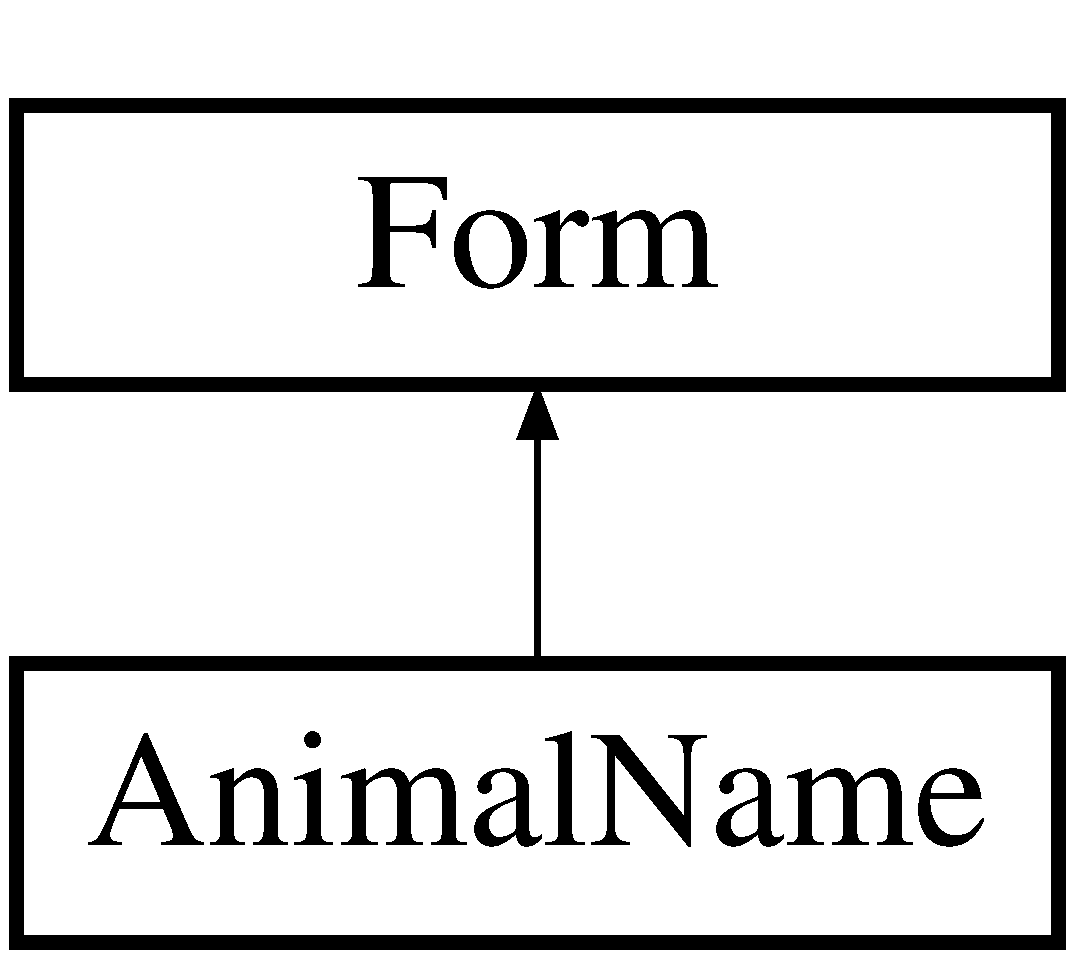
\includegraphics[height=2.000000cm]{classWildlifeTrackingApp_1_1AnimalName}
\end{center}
\end{figure}
\subsection*{Public Member Functions}
\begin{DoxyCompactItemize}
\item 
\hyperlink{classWildlifeTrackingApp_1_1AnimalName_a77c9c1ee4d566c59e85c75f4382ccb39}{Animal\+Name} ()
\end{DoxyCompactItemize}
\subsection*{Protected Member Functions}
\begin{DoxyCompactItemize}
\item 
override void \hyperlink{classWildlifeTrackingApp_1_1AnimalName_a849c3c7f8d08104f0cdb46bee9fe6389}{Dispose} (bool disposing)
\begin{DoxyCompactList}\small\item\em Clean up any resources being used. \end{DoxyCompactList}\end{DoxyCompactItemize}
\subsection*{Private Member Functions}
\begin{DoxyCompactItemize}
\item 
void \hyperlink{classWildlifeTrackingApp_1_1AnimalName_a6405d5db675d5338663195a4d12b4c9f}{Initialize\+Component} ()
\begin{DoxyCompactList}\small\item\em Required method for Designer support -\/ do not modify the contents of this method with the code editor. \end{DoxyCompactList}\end{DoxyCompactItemize}
\subsection*{Private Attributes}
\begin{DoxyCompactItemize}
\item 
System.\+Windows.\+Forms.\+Text\+Box \hyperlink{classWildlifeTrackingApp_1_1AnimalName_abb2c1d4dd8e970c30d810f5238785813}{animal\+Name\+\_\+text\+Box}
\item 
System.\+Component\+Model.\+I\+Container \hyperlink{classWildlifeTrackingApp_1_1AnimalName_a02595f1c09713bb71dcb2fbbfc7ffa4b}{components} = null
\begin{DoxyCompactList}\small\item\em Required designer variable. \end{DoxyCompactList}\item 
System.\+Windows.\+Forms.\+Button \hyperlink{classWildlifeTrackingApp_1_1AnimalName_a6c7fe113bfa091362451d2814c3c108a}{submit\+\_\+button}
\end{DoxyCompactItemize}


\subsection{Constructor \& Destructor Documentation}
\mbox{\Hypertarget{classWildlifeTrackingApp_1_1AnimalName_a77c9c1ee4d566c59e85c75f4382ccb39}\label{classWildlifeTrackingApp_1_1AnimalName_a77c9c1ee4d566c59e85c75f4382ccb39}} 
\index{Wildlife\+Tracking\+App\+::\+Animal\+Name@{Wildlife\+Tracking\+App\+::\+Animal\+Name}!Animal\+Name@{Animal\+Name}}
\index{Animal\+Name@{Animal\+Name}!Wildlife\+Tracking\+App\+::\+Animal\+Name@{Wildlife\+Tracking\+App\+::\+Animal\+Name}}
\subsubsection{\texorpdfstring{Animal\+Name()}{AnimalName()}}
{\footnotesize\ttfamily \hyperlink{classWildlifeTrackingApp_1_1AnimalName}{Animal\+Name} (\begin{DoxyParamCaption}{ }\end{DoxyParamCaption})\hspace{0.3cm}{\ttfamily [inline]}}



\subsection{Member Function Documentation}
\mbox{\Hypertarget{classWildlifeTrackingApp_1_1AnimalName_a849c3c7f8d08104f0cdb46bee9fe6389}\label{classWildlifeTrackingApp_1_1AnimalName_a849c3c7f8d08104f0cdb46bee9fe6389}} 
\index{Wildlife\+Tracking\+App\+::\+Animal\+Name@{Wildlife\+Tracking\+App\+::\+Animal\+Name}!Dispose@{Dispose}}
\index{Dispose@{Dispose}!Wildlife\+Tracking\+App\+::\+Animal\+Name@{Wildlife\+Tracking\+App\+::\+Animal\+Name}}
\subsubsection{\texorpdfstring{Dispose()}{Dispose()}}
{\footnotesize\ttfamily override void Dispose (\begin{DoxyParamCaption}\item[{bool}]{disposing }\end{DoxyParamCaption})\hspace{0.3cm}{\ttfamily [inline]}, {\ttfamily [protected]}}



Clean up any resources being used. 


\begin{DoxyParams}{Parameters}
{\em disposing} & true if managed resources should be disposed; otherwise, false.\\
\hline
\end{DoxyParams}
\mbox{\Hypertarget{classWildlifeTrackingApp_1_1AnimalName_a6405d5db675d5338663195a4d12b4c9f}\label{classWildlifeTrackingApp_1_1AnimalName_a6405d5db675d5338663195a4d12b4c9f}} 
\index{Wildlife\+Tracking\+App\+::\+Animal\+Name@{Wildlife\+Tracking\+App\+::\+Animal\+Name}!Initialize\+Component@{Initialize\+Component}}
\index{Initialize\+Component@{Initialize\+Component}!Wildlife\+Tracking\+App\+::\+Animal\+Name@{Wildlife\+Tracking\+App\+::\+Animal\+Name}}
\subsubsection{\texorpdfstring{Initialize\+Component()}{InitializeComponent()}}
{\footnotesize\ttfamily void Initialize\+Component (\begin{DoxyParamCaption}{ }\end{DoxyParamCaption})\hspace{0.3cm}{\ttfamily [inline]}, {\ttfamily [private]}}



Required method for Designer support -\/ do not modify the contents of this method with the code editor. 



\subsection{Member Data Documentation}
\mbox{\Hypertarget{classWildlifeTrackingApp_1_1AnimalName_abb2c1d4dd8e970c30d810f5238785813}\label{classWildlifeTrackingApp_1_1AnimalName_abb2c1d4dd8e970c30d810f5238785813}} 
\index{Wildlife\+Tracking\+App\+::\+Animal\+Name@{Wildlife\+Tracking\+App\+::\+Animal\+Name}!animal\+Name\+\_\+text\+Box@{animal\+Name\+\_\+text\+Box}}
\index{animal\+Name\+\_\+text\+Box@{animal\+Name\+\_\+text\+Box}!Wildlife\+Tracking\+App\+::\+Animal\+Name@{Wildlife\+Tracking\+App\+::\+Animal\+Name}}
\subsubsection{\texorpdfstring{animal\+Name\+\_\+text\+Box}{animalName\_textBox}}
{\footnotesize\ttfamily System.\+Windows.\+Forms.\+Text\+Box animal\+Name\+\_\+text\+Box\hspace{0.3cm}{\ttfamily [private]}}

\mbox{\Hypertarget{classWildlifeTrackingApp_1_1AnimalName_a02595f1c09713bb71dcb2fbbfc7ffa4b}\label{classWildlifeTrackingApp_1_1AnimalName_a02595f1c09713bb71dcb2fbbfc7ffa4b}} 
\index{Wildlife\+Tracking\+App\+::\+Animal\+Name@{Wildlife\+Tracking\+App\+::\+Animal\+Name}!components@{components}}
\index{components@{components}!Wildlife\+Tracking\+App\+::\+Animal\+Name@{Wildlife\+Tracking\+App\+::\+Animal\+Name}}
\subsubsection{\texorpdfstring{components}{components}}
{\footnotesize\ttfamily System.\+Component\+Model.\+I\+Container components = null\hspace{0.3cm}{\ttfamily [private]}}



Required designer variable. 

\mbox{\Hypertarget{classWildlifeTrackingApp_1_1AnimalName_a6c7fe113bfa091362451d2814c3c108a}\label{classWildlifeTrackingApp_1_1AnimalName_a6c7fe113bfa091362451d2814c3c108a}} 
\index{Wildlife\+Tracking\+App\+::\+Animal\+Name@{Wildlife\+Tracking\+App\+::\+Animal\+Name}!submit\+\_\+button@{submit\+\_\+button}}
\index{submit\+\_\+button@{submit\+\_\+button}!Wildlife\+Tracking\+App\+::\+Animal\+Name@{Wildlife\+Tracking\+App\+::\+Animal\+Name}}
\subsubsection{\texorpdfstring{submit\+\_\+button}{submit\_button}}
{\footnotesize\ttfamily System.\+Windows.\+Forms.\+Button submit\+\_\+button\hspace{0.3cm}{\ttfamily [private]}}



The documentation for this class was generated from the following files\+:\begin{DoxyCompactItemize}
\item 
\hyperlink{AnimalName_8cs}{Animal\+Name.\+cs}\item 
\hyperlink{AnimalName_8Designer_8cs}{Animal\+Name.\+Designer.\+cs}\end{DoxyCompactItemize}

\hypertarget{classWildlifeTrackingApp_1_1Category}{}\section{Category}
\label{classWildlifeTrackingApp_1_1Category}\index{Category@{Category}}


Form class for showing the list of all categories, adding new category, deleting and editing category.  


Inheritance diagram for Category\+:\begin{figure}[H]
\begin{center}
\leavevmode
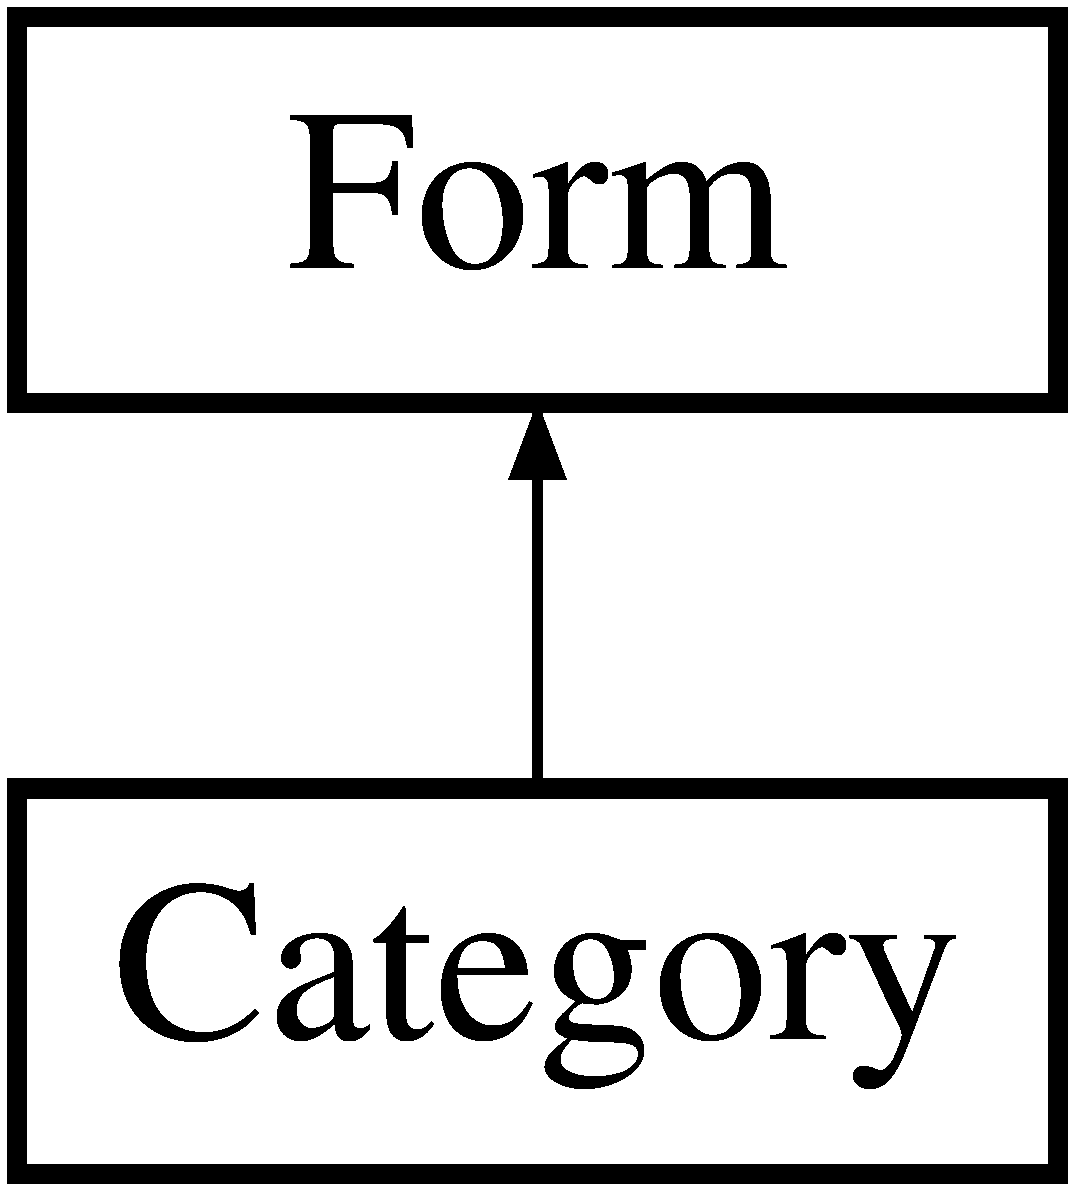
\includegraphics[height=2.000000cm]{classWildlifeTrackingApp_1_1Category}
\end{center}
\end{figure}
\subsection*{Public Member Functions}
\begin{DoxyCompactItemize}
\item 
\hyperlink{classWildlifeTrackingApp_1_1Category_a0e526c1d022adf4f003029e995a50ff7}{Category} ()
\end{DoxyCompactItemize}
\subsection*{Public Attributes}
\begin{DoxyCompactItemize}
\item 
int \hyperlink{classWildlifeTrackingApp_1_1Category_aad96a74a8e07bceb571a64a3355b779d}{selected\+Row}
\end{DoxyCompactItemize}
\subsection*{Protected Member Functions}
\begin{DoxyCompactItemize}
\item 
override void \hyperlink{classWildlifeTrackingApp_1_1Category_a849c3c7f8d08104f0cdb46bee9fe6389}{Dispose} (bool disposing)
\begin{DoxyCompactList}\small\item\em Clean up any resources being used. \end{DoxyCompactList}\end{DoxyCompactItemize}
\subsection*{Properties}
\begin{DoxyCompactItemize}
\item 
static log4net.\+I\+Log \hyperlink{classWildlifeTrackingApp_1_1Category_a5fc9abb86e6110ecd61d0a1a7d740a8a}{Log}\hspace{0.3cm}{\ttfamily  \mbox{[}get, private set\mbox{]}}
\end{DoxyCompactItemize}
\subsection*{Private Member Functions}
\begin{DoxyCompactItemize}
\item 
void \hyperlink{classWildlifeTrackingApp_1_1Category_ae56b21bee08f5cad9858a264ccc21fd5}{add\+\_\+button\+\_\+\+Click} (object sender, Event\+Args e)
\begin{DoxyCompactList}\small\item\em Event handler for add button click. It accept data and send it to server. \end{DoxyCompactList}\item 
void \hyperlink{classWildlifeTrackingApp_1_1Category_ad88debab69dc59b9a3bc2bdd89b1e4f9}{Category\+\_\+\+Activated} (object sender, Event\+Args e)
\begin{DoxyCompactList}\small\item\em Event handler for activation of form. \end{DoxyCompactList}\item 
void \hyperlink{classWildlifeTrackingApp_1_1Category_af87e0d54e9971bfe9ccba3a85841f619}{data\+Grid} ()
\begin{DoxyCompactList}\small\item\em It loads data to datagrid view. \end{DoxyCompactList}\item 
void \hyperlink{classWildlifeTrackingApp_1_1Category_a28f46cdb401c2c8da3f8e117eaedf977}{delete\+\_\+button\+\_\+\+Click} (object sender, Event\+Args e)
\begin{DoxyCompactList}\small\item\em Event handler for delete button click. \end{DoxyCompactList}\item 
void \hyperlink{classWildlifeTrackingApp_1_1Category_adef76d49a202d1276ec8ca56b5b0bd3b}{edit\+\_\+button\+\_\+\+Click} (object sender, Event\+Args e)
\begin{DoxyCompactList}\small\item\em Event handler for edit button click. \end{DoxyCompactList}\item 
\hyperlink{classWildlifeTrackingApp_1_1Models_1_1Category}{Models.\+Category} \hyperlink{classWildlifeTrackingApp_1_1Category_ad0b8994ac9ba019fb7cd6564e0ce4234}{Get\+Category} (string category\+Name, string category\+Color, string category\+Desc)
\item 
Data\+Table \hyperlink{classWildlifeTrackingApp_1_1Category_a8e22ded5eb81e2790b567eb19d3fe373}{Get\+R\+E\+S\+T\+Data} ()
\begin{DoxyCompactList}\small\item\em Collects categroy details and saves as a datatable. \end{DoxyCompactList}\item 
void \hyperlink{classWildlifeTrackingApp_1_1Category_a6405d5db675d5338663195a4d12b4c9f}{Initialize\+Component} ()
\begin{DoxyCompactList}\small\item\em Required method for Designer support -\/ do not modify the contents of this method with the code editor. \end{DoxyCompactList}\end{DoxyCompactItemize}
\subsection*{Private Attributes}
\begin{DoxyCompactItemize}
\item 
System.\+Windows.\+Forms.\+Button \hyperlink{classWildlifeTrackingApp_1_1Category_a7f1dbd5813451728f923cb88a3469cb6}{add\+\_\+button}
\item 
List$<$ \hyperlink{classWildlifeTrackingApp_1_1Models_1_1Category}{Models.\+Category} $>$ \hyperlink{classWildlifeTrackingApp_1_1Category_a02effa079a870eac99d658ab96077499}{all\+Category\+Details}
\item 
System.\+Windows.\+Forms.\+Data\+Grid\+View \hyperlink{classWildlifeTrackingApp_1_1Category_aca0b56eba54545e931661b3e3661c34b}{category\+\_\+data\+Grid\+View}
\item 
Data\+Table \hyperlink{classWildlifeTrackingApp_1_1Category_a205fdcaba6d0c0047179a287f02825cf}{category\+Detail}
\item 
System.\+Component\+Model.\+I\+Container \hyperlink{classWildlifeTrackingApp_1_1Category_a02595f1c09713bb71dcb2fbbfc7ffa4b}{components} = null
\begin{DoxyCompactList}\small\item\em Required designer variable. \end{DoxyCompactList}\item 
System.\+Windows.\+Forms.\+Button \hyperlink{classWildlifeTrackingApp_1_1Category_a84dcb7863c4f709001a644ff98f22414}{delete\+\_\+button}
\end{DoxyCompactItemize}
\subsection*{Static Private Attributes}
\begin{DoxyCompactItemize}
\item 
static readonly log4net.\+I\+Log \hyperlink{classWildlifeTrackingApp_1_1Category_ae6c6142b8525b2f4ac6ee6e003b3106f}{log}
\end{DoxyCompactItemize}


\subsection{Detailed Description}
Form class for showing the list of all categories, adding new category, deleting and editing category. 



\subsection{Constructor \& Destructor Documentation}
\mbox{\Hypertarget{classWildlifeTrackingApp_1_1Category_a0e526c1d022adf4f003029e995a50ff7}\label{classWildlifeTrackingApp_1_1Category_a0e526c1d022adf4f003029e995a50ff7}} 
\index{Wildlife\+Tracking\+App\+::\+Category@{Wildlife\+Tracking\+App\+::\+Category}!Category@{Category}}
\index{Category@{Category}!Wildlife\+Tracking\+App\+::\+Category@{Wildlife\+Tracking\+App\+::\+Category}}
\subsubsection{\texorpdfstring{Category()}{Category()}}
{\footnotesize\ttfamily \hyperlink{classWildlifeTrackingApp_1_1Category}{Category} (\begin{DoxyParamCaption}{ }\end{DoxyParamCaption})\hspace{0.3cm}{\ttfamily [inline]}}



\subsection{Member Function Documentation}
\mbox{\Hypertarget{classWildlifeTrackingApp_1_1Category_ae56b21bee08f5cad9858a264ccc21fd5}\label{classWildlifeTrackingApp_1_1Category_ae56b21bee08f5cad9858a264ccc21fd5}} 
\index{Wildlife\+Tracking\+App\+::\+Category@{Wildlife\+Tracking\+App\+::\+Category}!add\+\_\+button\+\_\+\+Click@{add\+\_\+button\+\_\+\+Click}}
\index{add\+\_\+button\+\_\+\+Click@{add\+\_\+button\+\_\+\+Click}!Wildlife\+Tracking\+App\+::\+Category@{Wildlife\+Tracking\+App\+::\+Category}}
\subsubsection{\texorpdfstring{add\+\_\+button\+\_\+\+Click()}{add\_button\_Click()}}
{\footnotesize\ttfamily void add\+\_\+button\+\_\+\+Click (\begin{DoxyParamCaption}\item[{object}]{sender,  }\item[{Event\+Args}]{e }\end{DoxyParamCaption})\hspace{0.3cm}{\ttfamily [inline]}, {\ttfamily [private]}}



Event handler for add button click. It accept data and send it to server. 


\begin{DoxyParams}{Parameters}
{\em sender} & \\
\hline
{\em e} & \\
\hline
\end{DoxyParams}
\mbox{\Hypertarget{classWildlifeTrackingApp_1_1Category_ad88debab69dc59b9a3bc2bdd89b1e4f9}\label{classWildlifeTrackingApp_1_1Category_ad88debab69dc59b9a3bc2bdd89b1e4f9}} 
\index{Wildlife\+Tracking\+App\+::\+Category@{Wildlife\+Tracking\+App\+::\+Category}!Category\+\_\+\+Activated@{Category\+\_\+\+Activated}}
\index{Category\+\_\+\+Activated@{Category\+\_\+\+Activated}!Wildlife\+Tracking\+App\+::\+Category@{Wildlife\+Tracking\+App\+::\+Category}}
\subsubsection{\texorpdfstring{Category\+\_\+\+Activated()}{Category\_Activated()}}
{\footnotesize\ttfamily void Category\+\_\+\+Activated (\begin{DoxyParamCaption}\item[{object}]{sender,  }\item[{Event\+Args}]{e }\end{DoxyParamCaption})\hspace{0.3cm}{\ttfamily [inline]}, {\ttfamily [private]}}



Event handler for activation of form. 


\begin{DoxyParams}{Parameters}
{\em sender} & Sender Object\\
\hline
{\em e} & Event Argument\\
\hline
\end{DoxyParams}
\mbox{\Hypertarget{classWildlifeTrackingApp_1_1Category_af87e0d54e9971bfe9ccba3a85841f619}\label{classWildlifeTrackingApp_1_1Category_af87e0d54e9971bfe9ccba3a85841f619}} 
\index{Wildlife\+Tracking\+App\+::\+Category@{Wildlife\+Tracking\+App\+::\+Category}!data\+Grid@{data\+Grid}}
\index{data\+Grid@{data\+Grid}!Wildlife\+Tracking\+App\+::\+Category@{Wildlife\+Tracking\+App\+::\+Category}}
\subsubsection{\texorpdfstring{data\+Grid()}{dataGrid()}}
{\footnotesize\ttfamily void data\+Grid (\begin{DoxyParamCaption}{ }\end{DoxyParamCaption})\hspace{0.3cm}{\ttfamily [inline]}, {\ttfamily [private]}}



It loads data to datagrid view. 

\mbox{\Hypertarget{classWildlifeTrackingApp_1_1Category_a28f46cdb401c2c8da3f8e117eaedf977}\label{classWildlifeTrackingApp_1_1Category_a28f46cdb401c2c8da3f8e117eaedf977}} 
\index{Wildlife\+Tracking\+App\+::\+Category@{Wildlife\+Tracking\+App\+::\+Category}!delete\+\_\+button\+\_\+\+Click@{delete\+\_\+button\+\_\+\+Click}}
\index{delete\+\_\+button\+\_\+\+Click@{delete\+\_\+button\+\_\+\+Click}!Wildlife\+Tracking\+App\+::\+Category@{Wildlife\+Tracking\+App\+::\+Category}}
\subsubsection{\texorpdfstring{delete\+\_\+button\+\_\+\+Click()}{delete\_button\_Click()}}
{\footnotesize\ttfamily void delete\+\_\+button\+\_\+\+Click (\begin{DoxyParamCaption}\item[{object}]{sender,  }\item[{Event\+Args}]{e }\end{DoxyParamCaption})\hspace{0.3cm}{\ttfamily [inline]}, {\ttfamily [private]}}



Event handler for delete button click. 


\begin{DoxyParams}{Parameters}
{\em sender} & Sender Object\\
\hline
{\em e} & Event argument\\
\hline
\end{DoxyParams}
\mbox{\Hypertarget{classWildlifeTrackingApp_1_1Category_a849c3c7f8d08104f0cdb46bee9fe6389}\label{classWildlifeTrackingApp_1_1Category_a849c3c7f8d08104f0cdb46bee9fe6389}} 
\index{Wildlife\+Tracking\+App\+::\+Category@{Wildlife\+Tracking\+App\+::\+Category}!Dispose@{Dispose}}
\index{Dispose@{Dispose}!Wildlife\+Tracking\+App\+::\+Category@{Wildlife\+Tracking\+App\+::\+Category}}
\subsubsection{\texorpdfstring{Dispose()}{Dispose()}}
{\footnotesize\ttfamily override void Dispose (\begin{DoxyParamCaption}\item[{bool}]{disposing }\end{DoxyParamCaption})\hspace{0.3cm}{\ttfamily [inline]}, {\ttfamily [protected]}}



Clean up any resources being used. 


\begin{DoxyParams}{Parameters}
{\em disposing} & true if managed resources should be disposed; otherwise, false.\\
\hline
\end{DoxyParams}
\mbox{\Hypertarget{classWildlifeTrackingApp_1_1Category_adef76d49a202d1276ec8ca56b5b0bd3b}\label{classWildlifeTrackingApp_1_1Category_adef76d49a202d1276ec8ca56b5b0bd3b}} 
\index{Wildlife\+Tracking\+App\+::\+Category@{Wildlife\+Tracking\+App\+::\+Category}!edit\+\_\+button\+\_\+\+Click@{edit\+\_\+button\+\_\+\+Click}}
\index{edit\+\_\+button\+\_\+\+Click@{edit\+\_\+button\+\_\+\+Click}!Wildlife\+Tracking\+App\+::\+Category@{Wildlife\+Tracking\+App\+::\+Category}}
\subsubsection{\texorpdfstring{edit\+\_\+button\+\_\+\+Click()}{edit\_button\_Click()}}
{\footnotesize\ttfamily void edit\+\_\+button\+\_\+\+Click (\begin{DoxyParamCaption}\item[{object}]{sender,  }\item[{Event\+Args}]{e }\end{DoxyParamCaption})\hspace{0.3cm}{\ttfamily [inline]}, {\ttfamily [private]}}



Event handler for edit button click. 


\begin{DoxyParams}{Parameters}
{\em sender} & Sender Object\\
\hline
{\em e} & Event argument\\
\hline
\end{DoxyParams}
\mbox{\Hypertarget{classWildlifeTrackingApp_1_1Category_ad0b8994ac9ba019fb7cd6564e0ce4234}\label{classWildlifeTrackingApp_1_1Category_ad0b8994ac9ba019fb7cd6564e0ce4234}} 
\index{Wildlife\+Tracking\+App\+::\+Category@{Wildlife\+Tracking\+App\+::\+Category}!Get\+Category@{Get\+Category}}
\index{Get\+Category@{Get\+Category}!Wildlife\+Tracking\+App\+::\+Category@{Wildlife\+Tracking\+App\+::\+Category}}
\subsubsection{\texorpdfstring{Get\+Category()}{GetCategory()}}
{\footnotesize\ttfamily \hyperlink{classWildlifeTrackingApp_1_1Models_1_1Category}{Models.\+Category} Get\+Category (\begin{DoxyParamCaption}\item[{string}]{category\+Name,  }\item[{string}]{category\+Color,  }\item[{string}]{category\+Desc }\end{DoxyParamCaption})\hspace{0.3cm}{\ttfamily [inline]}, {\ttfamily [private]}}

\mbox{\Hypertarget{classWildlifeTrackingApp_1_1Category_a8e22ded5eb81e2790b567eb19d3fe373}\label{classWildlifeTrackingApp_1_1Category_a8e22ded5eb81e2790b567eb19d3fe373}} 
\index{Wildlife\+Tracking\+App\+::\+Category@{Wildlife\+Tracking\+App\+::\+Category}!Get\+R\+E\+S\+T\+Data@{Get\+R\+E\+S\+T\+Data}}
\index{Get\+R\+E\+S\+T\+Data@{Get\+R\+E\+S\+T\+Data}!Wildlife\+Tracking\+App\+::\+Category@{Wildlife\+Tracking\+App\+::\+Category}}
\subsubsection{\texorpdfstring{Get\+R\+E\+S\+T\+Data()}{GetRESTData()}}
{\footnotesize\ttfamily Data\+Table Get\+R\+E\+S\+T\+Data (\begin{DoxyParamCaption}{ }\end{DoxyParamCaption})\hspace{0.3cm}{\ttfamily [inline]}, {\ttfamily [private]}}



Collects categroy details and saves as a datatable. 

\begin{DoxyReturn}{Returns}
Returns category data as datatable
\end{DoxyReturn}
\mbox{\Hypertarget{classWildlifeTrackingApp_1_1Category_a6405d5db675d5338663195a4d12b4c9f}\label{classWildlifeTrackingApp_1_1Category_a6405d5db675d5338663195a4d12b4c9f}} 
\index{Wildlife\+Tracking\+App\+::\+Category@{Wildlife\+Tracking\+App\+::\+Category}!Initialize\+Component@{Initialize\+Component}}
\index{Initialize\+Component@{Initialize\+Component}!Wildlife\+Tracking\+App\+::\+Category@{Wildlife\+Tracking\+App\+::\+Category}}
\subsubsection{\texorpdfstring{Initialize\+Component()}{InitializeComponent()}}
{\footnotesize\ttfamily void Initialize\+Component (\begin{DoxyParamCaption}{ }\end{DoxyParamCaption})\hspace{0.3cm}{\ttfamily [inline]}, {\ttfamily [private]}}



Required method for Designer support -\/ do not modify the contents of this method with the code editor. 



\subsection{Member Data Documentation}
\mbox{\Hypertarget{classWildlifeTrackingApp_1_1Category_a7f1dbd5813451728f923cb88a3469cb6}\label{classWildlifeTrackingApp_1_1Category_a7f1dbd5813451728f923cb88a3469cb6}} 
\index{Wildlife\+Tracking\+App\+::\+Category@{Wildlife\+Tracking\+App\+::\+Category}!add\+\_\+button@{add\+\_\+button}}
\index{add\+\_\+button@{add\+\_\+button}!Wildlife\+Tracking\+App\+::\+Category@{Wildlife\+Tracking\+App\+::\+Category}}
\subsubsection{\texorpdfstring{add\+\_\+button}{add\_button}}
{\footnotesize\ttfamily System.\+Windows.\+Forms.\+Button add\+\_\+button\hspace{0.3cm}{\ttfamily [private]}}

\mbox{\Hypertarget{classWildlifeTrackingApp_1_1Category_a02effa079a870eac99d658ab96077499}\label{classWildlifeTrackingApp_1_1Category_a02effa079a870eac99d658ab96077499}} 
\index{Wildlife\+Tracking\+App\+::\+Category@{Wildlife\+Tracking\+App\+::\+Category}!all\+Category\+Details@{all\+Category\+Details}}
\index{all\+Category\+Details@{all\+Category\+Details}!Wildlife\+Tracking\+App\+::\+Category@{Wildlife\+Tracking\+App\+::\+Category}}
\subsubsection{\texorpdfstring{all\+Category\+Details}{allCategoryDetails}}
{\footnotesize\ttfamily List$<$\hyperlink{classWildlifeTrackingApp_1_1Models_1_1Category}{Models.\+Category}$>$ all\+Category\+Details\hspace{0.3cm}{\ttfamily [private]}}

\mbox{\Hypertarget{classWildlifeTrackingApp_1_1Category_aca0b56eba54545e931661b3e3661c34b}\label{classWildlifeTrackingApp_1_1Category_aca0b56eba54545e931661b3e3661c34b}} 
\index{Wildlife\+Tracking\+App\+::\+Category@{Wildlife\+Tracking\+App\+::\+Category}!category\+\_\+data\+Grid\+View@{category\+\_\+data\+Grid\+View}}
\index{category\+\_\+data\+Grid\+View@{category\+\_\+data\+Grid\+View}!Wildlife\+Tracking\+App\+::\+Category@{Wildlife\+Tracking\+App\+::\+Category}}
\subsubsection{\texorpdfstring{category\+\_\+data\+Grid\+View}{category\_dataGridView}}
{\footnotesize\ttfamily System.\+Windows.\+Forms.\+Data\+Grid\+View category\+\_\+data\+Grid\+View\hspace{0.3cm}{\ttfamily [private]}}

\mbox{\Hypertarget{classWildlifeTrackingApp_1_1Category_a205fdcaba6d0c0047179a287f02825cf}\label{classWildlifeTrackingApp_1_1Category_a205fdcaba6d0c0047179a287f02825cf}} 
\index{Wildlife\+Tracking\+App\+::\+Category@{Wildlife\+Tracking\+App\+::\+Category}!category\+Detail@{category\+Detail}}
\index{category\+Detail@{category\+Detail}!Wildlife\+Tracking\+App\+::\+Category@{Wildlife\+Tracking\+App\+::\+Category}}
\subsubsection{\texorpdfstring{category\+Detail}{categoryDetail}}
{\footnotesize\ttfamily Data\+Table category\+Detail\hspace{0.3cm}{\ttfamily [private]}}

\mbox{\Hypertarget{classWildlifeTrackingApp_1_1Category_a02595f1c09713bb71dcb2fbbfc7ffa4b}\label{classWildlifeTrackingApp_1_1Category_a02595f1c09713bb71dcb2fbbfc7ffa4b}} 
\index{Wildlife\+Tracking\+App\+::\+Category@{Wildlife\+Tracking\+App\+::\+Category}!components@{components}}
\index{components@{components}!Wildlife\+Tracking\+App\+::\+Category@{Wildlife\+Tracking\+App\+::\+Category}}
\subsubsection{\texorpdfstring{components}{components}}
{\footnotesize\ttfamily System.\+Component\+Model.\+I\+Container components = null\hspace{0.3cm}{\ttfamily [private]}}



Required designer variable. 

\mbox{\Hypertarget{classWildlifeTrackingApp_1_1Category_a84dcb7863c4f709001a644ff98f22414}\label{classWildlifeTrackingApp_1_1Category_a84dcb7863c4f709001a644ff98f22414}} 
\index{Wildlife\+Tracking\+App\+::\+Category@{Wildlife\+Tracking\+App\+::\+Category}!delete\+\_\+button@{delete\+\_\+button}}
\index{delete\+\_\+button@{delete\+\_\+button}!Wildlife\+Tracking\+App\+::\+Category@{Wildlife\+Tracking\+App\+::\+Category}}
\subsubsection{\texorpdfstring{delete\+\_\+button}{delete\_button}}
{\footnotesize\ttfamily System.\+Windows.\+Forms.\+Button delete\+\_\+button\hspace{0.3cm}{\ttfamily [private]}}

\mbox{\Hypertarget{classWildlifeTrackingApp_1_1Category_ae6c6142b8525b2f4ac6ee6e003b3106f}\label{classWildlifeTrackingApp_1_1Category_ae6c6142b8525b2f4ac6ee6e003b3106f}} 
\index{Wildlife\+Tracking\+App\+::\+Category@{Wildlife\+Tracking\+App\+::\+Category}!log@{log}}
\index{log@{log}!Wildlife\+Tracking\+App\+::\+Category@{Wildlife\+Tracking\+App\+::\+Category}}
\subsubsection{\texorpdfstring{log}{log}}
{\footnotesize\ttfamily readonly log4net.\+I\+Log log\hspace{0.3cm}{\ttfamily [static]}, {\ttfamily [private]}}

{\bfseries Initial value\+:}
\begin{DoxyCode}
= log4net.LogManager.GetLogger
        (\hyperlink{namespaceSystem}{System}.Reflection.MethodBase.GetCurrentMethod().DeclaringType)
\end{DoxyCode}
\mbox{\Hypertarget{classWildlifeTrackingApp_1_1Category_aad96a74a8e07bceb571a64a3355b779d}\label{classWildlifeTrackingApp_1_1Category_aad96a74a8e07bceb571a64a3355b779d}} 
\index{Wildlife\+Tracking\+App\+::\+Category@{Wildlife\+Tracking\+App\+::\+Category}!selected\+Row@{selected\+Row}}
\index{selected\+Row@{selected\+Row}!Wildlife\+Tracking\+App\+::\+Category@{Wildlife\+Tracking\+App\+::\+Category}}
\subsubsection{\texorpdfstring{selected\+Row}{selectedRow}}
{\footnotesize\ttfamily int selected\+Row}



\subsection{Property Documentation}
\mbox{\Hypertarget{classWildlifeTrackingApp_1_1Category_a5fc9abb86e6110ecd61d0a1a7d740a8a}\label{classWildlifeTrackingApp_1_1Category_a5fc9abb86e6110ecd61d0a1a7d740a8a}} 
\index{Wildlife\+Tracking\+App\+::\+Category@{Wildlife\+Tracking\+App\+::\+Category}!Log@{Log}}
\index{Log@{Log}!Wildlife\+Tracking\+App\+::\+Category@{Wildlife\+Tracking\+App\+::\+Category}}
\subsubsection{\texorpdfstring{Log}{Log}}
{\footnotesize\ttfamily log4net.\+I\+Log Log\hspace{0.3cm}{\ttfamily [static]}, {\ttfamily [get]}, {\ttfamily [private set]}}



The documentation for this class was generated from the following files\+:\begin{DoxyCompactItemize}
\item 
View/\hyperlink{View_2Category_8cs}{Category.\+cs}\item 
View/\hyperlink{Category_8Designer_8cs}{Category.\+Designer.\+cs}\end{DoxyCompactItemize}

\hypertarget{classWildlifeTrackingApp_1_1Delegates_1_1AnimalDelegate}{}\section{Animal\+Delegate}
\label{classWildlifeTrackingApp_1_1Delegates_1_1AnimalDelegate}\index{Animal\+Delegate@{Animal\+Delegate}}


Class that calls server for adding new animal, getting animal details.  


\subsection*{Static Public Member Functions}
\begin{DoxyCompactItemize}
\item 
static \hyperlink{classWildlifeTrackingApp_1_1Models_1_1Animal}{Models.\+Animal} \hyperlink{classWildlifeTrackingApp_1_1Delegates_1_1AnimalDelegate_a57a5b0f9728b68e90dd1aa38ebd9df14}{Add\+New\+Animal} (\hyperlink{classWildlifeTrackingApp_1_1Models_1_1Animal}{Models.\+Animal} animal\+Details)
\begin{DoxyCompactList}\small\item\em Post call for adding new animal to the database. \end{DoxyCompactList}\item 
static \hyperlink{classWildlifeTrackingApp_1_1Models_1_1Animal}{Models.\+Animal} \hyperlink{classWildlifeTrackingApp_1_1Delegates_1_1AnimalDelegate_a9261f08d6ea296a3ea3b63256c299770}{Delete\+Animal} (int animal\+Id)
\begin{DoxyCompactList}\small\item\em Delete request for deleting the details of a particular animal. \end{DoxyCompactList}\item 
static List$<$ \hyperlink{classWildlifeTrackingApp_1_1Models_1_1Animal}{Models.\+Animal} $>$ \hyperlink{classWildlifeTrackingApp_1_1Delegates_1_1AnimalDelegate_acdcd9b138229c5e197e45cdad4025bad}{Get\+All\+Animals\+Allocated} ()
\begin{DoxyCompactList}\small\item\em Get call for getting the details of all animals. \end{DoxyCompactList}\item 
static List$<$ \hyperlink{classWildlifeTrackingApp_1_1Models_1_1AnimalCategoryCount}{Models.\+Animal\+Category\+Count} $>$ \hyperlink{classWildlifeTrackingApp_1_1Delegates_1_1AnimalDelegate_a2fd0ae1a6560b820addb282b1e6e4ad3}{Get\+Animals\+Count\+Per\+Category} (string from\+Date, string to\+Date)
\begin{DoxyCompactList}\small\item\em Get call for getting total count of all animals per category. \end{DoxyCompactList}\end{DoxyCompactItemize}


\subsection{Detailed Description}
Class that calls server for adding new animal, getting animal details. 



\subsection{Member Function Documentation}
\mbox{\Hypertarget{classWildlifeTrackingApp_1_1Delegates_1_1AnimalDelegate_a57a5b0f9728b68e90dd1aa38ebd9df14}\label{classWildlifeTrackingApp_1_1Delegates_1_1AnimalDelegate_a57a5b0f9728b68e90dd1aa38ebd9df14}} 
\index{Wildlife\+Tracking\+App\+::\+Delegates\+::\+Animal\+Delegate@{Wildlife\+Tracking\+App\+::\+Delegates\+::\+Animal\+Delegate}!Add\+New\+Animal@{Add\+New\+Animal}}
\index{Add\+New\+Animal@{Add\+New\+Animal}!Wildlife\+Tracking\+App\+::\+Delegates\+::\+Animal\+Delegate@{Wildlife\+Tracking\+App\+::\+Delegates\+::\+Animal\+Delegate}}
\subsubsection{\texorpdfstring{Add\+New\+Animal()}{AddNewAnimal()}}
{\footnotesize\ttfamily static \hyperlink{classWildlifeTrackingApp_1_1Models_1_1Animal}{Models.\+Animal} Add\+New\+Animal (\begin{DoxyParamCaption}\item[{\hyperlink{classWildlifeTrackingApp_1_1Models_1_1Animal}{Models.\+Animal}}]{animal\+Details }\end{DoxyParamCaption})\hspace{0.3cm}{\ttfamily [inline]}, {\ttfamily [static]}}



Post call for adding new animal to the database. 


\begin{DoxyParams}{Parameters}
{\em animal\+Details} & Instances of \hyperlink{classWildlifeTrackingApp_1_1Models_1_1Animal}{Models.\+Animal}\\
\hline
\end{DoxyParams}
\begin{DoxyReturn}{Returns}
Return instance of \hyperlink{classWildlifeTrackingApp_1_1Models_1_1Animal}{Models.\+Animal}
\end{DoxyReturn}
\mbox{\Hypertarget{classWildlifeTrackingApp_1_1Delegates_1_1AnimalDelegate_a9261f08d6ea296a3ea3b63256c299770}\label{classWildlifeTrackingApp_1_1Delegates_1_1AnimalDelegate_a9261f08d6ea296a3ea3b63256c299770}} 
\index{Wildlife\+Tracking\+App\+::\+Delegates\+::\+Animal\+Delegate@{Wildlife\+Tracking\+App\+::\+Delegates\+::\+Animal\+Delegate}!Delete\+Animal@{Delete\+Animal}}
\index{Delete\+Animal@{Delete\+Animal}!Wildlife\+Tracking\+App\+::\+Delegates\+::\+Animal\+Delegate@{Wildlife\+Tracking\+App\+::\+Delegates\+::\+Animal\+Delegate}}
\subsubsection{\texorpdfstring{Delete\+Animal()}{DeleteAnimal()}}
{\footnotesize\ttfamily static \hyperlink{classWildlifeTrackingApp_1_1Models_1_1Animal}{Models.\+Animal} Delete\+Animal (\begin{DoxyParamCaption}\item[{int}]{animal\+Id }\end{DoxyParamCaption})\hspace{0.3cm}{\ttfamily [inline]}, {\ttfamily [static]}}



Delete request for deleting the details of a particular animal. 


\begin{DoxyParams}{Parameters}
{\em animal\+Id} & Id of animal\\
\hline
\end{DoxyParams}
\begin{DoxyReturn}{Returns}
Return instance of \hyperlink{classWildlifeTrackingApp_1_1Models_1_1Animal}{Models.\+Animal}
\end{DoxyReturn}
\mbox{\Hypertarget{classWildlifeTrackingApp_1_1Delegates_1_1AnimalDelegate_acdcd9b138229c5e197e45cdad4025bad}\label{classWildlifeTrackingApp_1_1Delegates_1_1AnimalDelegate_acdcd9b138229c5e197e45cdad4025bad}} 
\index{Wildlife\+Tracking\+App\+::\+Delegates\+::\+Animal\+Delegate@{Wildlife\+Tracking\+App\+::\+Delegates\+::\+Animal\+Delegate}!Get\+All\+Animals\+Allocated@{Get\+All\+Animals\+Allocated}}
\index{Get\+All\+Animals\+Allocated@{Get\+All\+Animals\+Allocated}!Wildlife\+Tracking\+App\+::\+Delegates\+::\+Animal\+Delegate@{Wildlife\+Tracking\+App\+::\+Delegates\+::\+Animal\+Delegate}}
\subsubsection{\texorpdfstring{Get\+All\+Animals\+Allocated()}{GetAllAnimalsAllocated()}}
{\footnotesize\ttfamily static List$<$\hyperlink{classWildlifeTrackingApp_1_1Models_1_1Animal}{Models.\+Animal}$>$ Get\+All\+Animals\+Allocated (\begin{DoxyParamCaption}{ }\end{DoxyParamCaption})\hspace{0.3cm}{\ttfamily [inline]}, {\ttfamily [static]}}



Get call for getting the details of all animals. 

\begin{DoxyReturn}{Returns}
Return list of instances of \hyperlink{classWildlifeTrackingApp_1_1Models_1_1Animal}{Models.\+Animal}
\end{DoxyReturn}
\mbox{\Hypertarget{classWildlifeTrackingApp_1_1Delegates_1_1AnimalDelegate_a2fd0ae1a6560b820addb282b1e6e4ad3}\label{classWildlifeTrackingApp_1_1Delegates_1_1AnimalDelegate_a2fd0ae1a6560b820addb282b1e6e4ad3}} 
\index{Wildlife\+Tracking\+App\+::\+Delegates\+::\+Animal\+Delegate@{Wildlife\+Tracking\+App\+::\+Delegates\+::\+Animal\+Delegate}!Get\+Animals\+Count\+Per\+Category@{Get\+Animals\+Count\+Per\+Category}}
\index{Get\+Animals\+Count\+Per\+Category@{Get\+Animals\+Count\+Per\+Category}!Wildlife\+Tracking\+App\+::\+Delegates\+::\+Animal\+Delegate@{Wildlife\+Tracking\+App\+::\+Delegates\+::\+Animal\+Delegate}}
\subsubsection{\texorpdfstring{Get\+Animals\+Count\+Per\+Category()}{GetAnimalsCountPerCategory()}}
{\footnotesize\ttfamily static List$<$\hyperlink{classWildlifeTrackingApp_1_1Models_1_1AnimalCategoryCount}{Models.\+Animal\+Category\+Count}$>$ Get\+Animals\+Count\+Per\+Category (\begin{DoxyParamCaption}\item[{string}]{from\+Date,  }\item[{string}]{to\+Date }\end{DoxyParamCaption})\hspace{0.3cm}{\ttfamily [inline]}, {\ttfamily [static]}}



Get call for getting total count of all animals per category. 


\begin{DoxyParams}{Parameters}
{\em from\+Date} & From date\\
\hline
{\em to\+Date} & To date\\
\hline
\end{DoxyParams}
\begin{DoxyReturn}{Returns}
Return instance of \hyperlink{classWildlifeTrackingApp_1_1Models_1_1Animal}{Models.\+Animal}
\end{DoxyReturn}


The documentation for this class was generated from the following file\+:\begin{DoxyCompactItemize}
\item 
Delegates/\hyperlink{AnimalDelegate_8cs}{Animal\+Delegate.\+cs}\end{DoxyCompactItemize}

\hypertarget{classWildlifeTrackingApp_1_1Delegates_1_1CategoryDelegate}{}\section{Category\+Delegate}
\label{classWildlifeTrackingApp_1_1Delegates_1_1CategoryDelegate}\index{Category\+Delegate@{Category\+Delegate}}


Class that calls server to get the details about different categories, delete categories,..  


\subsection*{Static Public Member Functions}
\begin{DoxyCompactItemize}
\item 
static \hyperlink{classWildlifeTrackingApp_1_1Models_1_1Category}{Models.\+Category} \hyperlink{classWildlifeTrackingApp_1_1Delegates_1_1CategoryDelegate_addca73f407ae2c8d31d5b19067e6dce7}{Add\+New\+Category} (\hyperlink{classWildlifeTrackingApp_1_1Models_1_1Category}{Models.\+Category} category\+Details)
\begin{DoxyCompactList}\small\item\em Post call for adding details of new category. \end{DoxyCompactList}\item 
static \hyperlink{classWildlifeTrackingApp_1_1Models_1_1Category}{Models.\+Category} \hyperlink{classWildlifeTrackingApp_1_1Delegates_1_1CategoryDelegate_ad3b0dad81563543b37fd3cc8688de0c7}{Delete\+Category} (int category\+Id)
\begin{DoxyCompactList}\small\item\em Delete call for deleting details of all categories. \end{DoxyCompactList}\item 
static List$<$ \hyperlink{classWildlifeTrackingApp_1_1Models_1_1Category}{Models.\+Category} $>$ \hyperlink{classWildlifeTrackingApp_1_1Delegates_1_1CategoryDelegate_a8c9a78152f0a7e86dc3ea0b828cdfd77}{Get\+All\+Categories} ()
\begin{DoxyCompactList}\small\item\em Get call for getting details of all categories. \end{DoxyCompactList}\end{DoxyCompactItemize}


\subsection{Detailed Description}
Class that calls server to get the details about different categories, delete categories,.. 



\subsection{Member Function Documentation}
\mbox{\Hypertarget{classWildlifeTrackingApp_1_1Delegates_1_1CategoryDelegate_addca73f407ae2c8d31d5b19067e6dce7}\label{classWildlifeTrackingApp_1_1Delegates_1_1CategoryDelegate_addca73f407ae2c8d31d5b19067e6dce7}} 
\index{Wildlife\+Tracking\+App\+::\+Delegates\+::\+Category\+Delegate@{Wildlife\+Tracking\+App\+::\+Delegates\+::\+Category\+Delegate}!Add\+New\+Category@{Add\+New\+Category}}
\index{Add\+New\+Category@{Add\+New\+Category}!Wildlife\+Tracking\+App\+::\+Delegates\+::\+Category\+Delegate@{Wildlife\+Tracking\+App\+::\+Delegates\+::\+Category\+Delegate}}
\subsubsection{\texorpdfstring{Add\+New\+Category()}{AddNewCategory()}}
{\footnotesize\ttfamily static \hyperlink{classWildlifeTrackingApp_1_1Models_1_1Category}{Models.\+Category} Add\+New\+Category (\begin{DoxyParamCaption}\item[{\hyperlink{classWildlifeTrackingApp_1_1Models_1_1Category}{Models.\+Category}}]{category\+Details }\end{DoxyParamCaption})\hspace{0.3cm}{\ttfamily [inline]}, {\ttfamily [static]}}



Post call for adding details of new category. 


\begin{DoxyParams}{Parameters}
{\em category\+Details} & instances of \hyperlink{classWildlifeTrackingApp_1_1Models_1_1Category}{Models.\+Category}\\
\hline
\end{DoxyParams}
\begin{DoxyReturn}{Returns}
Returns list of instance of \hyperlink{classWildlifeTrackingApp_1_1Models_1_1Category}{Models.\+Category}
\end{DoxyReturn}
\mbox{\Hypertarget{classWildlifeTrackingApp_1_1Delegates_1_1CategoryDelegate_ad3b0dad81563543b37fd3cc8688de0c7}\label{classWildlifeTrackingApp_1_1Delegates_1_1CategoryDelegate_ad3b0dad81563543b37fd3cc8688de0c7}} 
\index{Wildlife\+Tracking\+App\+::\+Delegates\+::\+Category\+Delegate@{Wildlife\+Tracking\+App\+::\+Delegates\+::\+Category\+Delegate}!Delete\+Category@{Delete\+Category}}
\index{Delete\+Category@{Delete\+Category}!Wildlife\+Tracking\+App\+::\+Delegates\+::\+Category\+Delegate@{Wildlife\+Tracking\+App\+::\+Delegates\+::\+Category\+Delegate}}
\subsubsection{\texorpdfstring{Delete\+Category()}{DeleteCategory()}}
{\footnotesize\ttfamily static \hyperlink{classWildlifeTrackingApp_1_1Models_1_1Category}{Models.\+Category} Delete\+Category (\begin{DoxyParamCaption}\item[{int}]{category\+Id }\end{DoxyParamCaption})\hspace{0.3cm}{\ttfamily [inline]}, {\ttfamily [static]}}



Delete call for deleting details of all categories. 


\begin{DoxyParams}{Parameters}
{\em category\+Id} & Unique id cprresponding to each category.\\
\hline
\end{DoxyParams}
\begin{DoxyReturn}{Returns}
Returns list of instance of \hyperlink{classWildlifeTrackingApp_1_1Models_1_1Category}{Models.\+Category}
\end{DoxyReturn}
\mbox{\Hypertarget{classWildlifeTrackingApp_1_1Delegates_1_1CategoryDelegate_a8c9a78152f0a7e86dc3ea0b828cdfd77}\label{classWildlifeTrackingApp_1_1Delegates_1_1CategoryDelegate_a8c9a78152f0a7e86dc3ea0b828cdfd77}} 
\index{Wildlife\+Tracking\+App\+::\+Delegates\+::\+Category\+Delegate@{Wildlife\+Tracking\+App\+::\+Delegates\+::\+Category\+Delegate}!Get\+All\+Categories@{Get\+All\+Categories}}
\index{Get\+All\+Categories@{Get\+All\+Categories}!Wildlife\+Tracking\+App\+::\+Delegates\+::\+Category\+Delegate@{Wildlife\+Tracking\+App\+::\+Delegates\+::\+Category\+Delegate}}
\subsubsection{\texorpdfstring{Get\+All\+Categories()}{GetAllCategories()}}
{\footnotesize\ttfamily static List$<$\hyperlink{classWildlifeTrackingApp_1_1Models_1_1Category}{Models.\+Category}$>$ Get\+All\+Categories (\begin{DoxyParamCaption}{ }\end{DoxyParamCaption})\hspace{0.3cm}{\ttfamily [inline]}, {\ttfamily [static]}}



Get call for getting details of all categories. 

\begin{DoxyReturn}{Returns}
Returns list of instances of \hyperlink{classWildlifeTrackingApp_1_1Models_1_1Category}{Models.\+Category}
\end{DoxyReturn}


The documentation for this class was generated from the following file\+:\begin{DoxyCompactItemize}
\item 
Delegates/\hyperlink{CategoryDelegate_8cs}{Category\+Delegate.\+cs}\end{DoxyCompactItemize}

\hypertarget{classWildlifeTrackingApp_1_1Delegates_1_1TrackingInfoDelegate}{}\section{Tracking\+Info\+Delegate}
\label{classWildlifeTrackingApp_1_1Delegates_1_1TrackingInfoDelegate}\index{Tracking\+Info\+Delegate@{Tracking\+Info\+Delegate}}


Class that call server to get the latest positions of different animals.  


\subsection*{Static Public Member Functions}
\begin{DoxyCompactItemize}
\item 
static List$<$ \hyperlink{classWildlifeTrackingApp_1_1Models_1_1TrackingInfo}{Tracking\+Info} $>$ \hyperlink{classWildlifeTrackingApp_1_1Delegates_1_1TrackingInfoDelegate_a1011cec68e4e27e80b5db0475f395768}{Get\+Latest\+Position\+Of\+All\+Animal} ()
\begin{DoxyCompactList}\small\item\em Gets the latest positions of all animals from all categories from the database through server call. \end{DoxyCompactList}\item 
static List$<$ \hyperlink{classWildlifeTrackingApp_1_1Models_1_1TrackingInfo}{Tracking\+Info} $>$ \hyperlink{classWildlifeTrackingApp_1_1Delegates_1_1TrackingInfoDelegate_a4ee9025a6305396144c0feff956de558}{Get\+Latest\+Position\+Of\+All\+Animal\+Per\+Category} (int category\+Id)
\begin{DoxyCompactList}\small\item\em Gets the latest positions of all animals from a particular category from the database through server call. \end{DoxyCompactList}\end{DoxyCompactItemize}


\subsection{Detailed Description}
Class that call server to get the latest positions of different animals. 



\subsection{Member Function Documentation}
\mbox{\Hypertarget{classWildlifeTrackingApp_1_1Delegates_1_1TrackingInfoDelegate_a1011cec68e4e27e80b5db0475f395768}\label{classWildlifeTrackingApp_1_1Delegates_1_1TrackingInfoDelegate_a1011cec68e4e27e80b5db0475f395768}} 
\index{Wildlife\+Tracking\+App\+::\+Delegates\+::\+Tracking\+Info\+Delegate@{Wildlife\+Tracking\+App\+::\+Delegates\+::\+Tracking\+Info\+Delegate}!Get\+Latest\+Position\+Of\+All\+Animal@{Get\+Latest\+Position\+Of\+All\+Animal}}
\index{Get\+Latest\+Position\+Of\+All\+Animal@{Get\+Latest\+Position\+Of\+All\+Animal}!Wildlife\+Tracking\+App\+::\+Delegates\+::\+Tracking\+Info\+Delegate@{Wildlife\+Tracking\+App\+::\+Delegates\+::\+Tracking\+Info\+Delegate}}
\subsubsection{\texorpdfstring{Get\+Latest\+Position\+Of\+All\+Animal()}{GetLatestPositionOfAllAnimal()}}
{\footnotesize\ttfamily static List$<$\hyperlink{classWildlifeTrackingApp_1_1Models_1_1TrackingInfo}{Tracking\+Info}$>$ Get\+Latest\+Position\+Of\+All\+Animal (\begin{DoxyParamCaption}{ }\end{DoxyParamCaption})\hspace{0.3cm}{\ttfamily [inline]}, {\ttfamily [static]}}



Gets the latest positions of all animals from all categories from the database through server call. 

\begin{DoxyReturn}{Returns}
Returns list of instances of Tracking\+Info class.
\end{DoxyReturn}
\mbox{\Hypertarget{classWildlifeTrackingApp_1_1Delegates_1_1TrackingInfoDelegate_a4ee9025a6305396144c0feff956de558}\label{classWildlifeTrackingApp_1_1Delegates_1_1TrackingInfoDelegate_a4ee9025a6305396144c0feff956de558}} 
\index{Wildlife\+Tracking\+App\+::\+Delegates\+::\+Tracking\+Info\+Delegate@{Wildlife\+Tracking\+App\+::\+Delegates\+::\+Tracking\+Info\+Delegate}!Get\+Latest\+Position\+Of\+All\+Animal\+Per\+Category@{Get\+Latest\+Position\+Of\+All\+Animal\+Per\+Category}}
\index{Get\+Latest\+Position\+Of\+All\+Animal\+Per\+Category@{Get\+Latest\+Position\+Of\+All\+Animal\+Per\+Category}!Wildlife\+Tracking\+App\+::\+Delegates\+::\+Tracking\+Info\+Delegate@{Wildlife\+Tracking\+App\+::\+Delegates\+::\+Tracking\+Info\+Delegate}}
\subsubsection{\texorpdfstring{Get\+Latest\+Position\+Of\+All\+Animal\+Per\+Category()}{GetLatestPositionOfAllAnimalPerCategory()}}
{\footnotesize\ttfamily static List$<$\hyperlink{classWildlifeTrackingApp_1_1Models_1_1TrackingInfo}{Tracking\+Info}$>$ Get\+Latest\+Position\+Of\+All\+Animal\+Per\+Category (\begin{DoxyParamCaption}\item[{int}]{category\+Id }\end{DoxyParamCaption})\hspace{0.3cm}{\ttfamily [inline]}, {\ttfamily [static]}}



Gets the latest positions of all animals from a particular category from the database through server call. 

\begin{DoxyReturn}{Returns}
Returns list of instances of Tracking\+Info class.
\end{DoxyReturn}


The documentation for this class was generated from the following file\+:\begin{DoxyCompactItemize}
\item 
Delegates/\hyperlink{TrackingInfoDelegate_8cs}{Tracking\+Info\+Delegate.\+cs}\end{DoxyCompactItemize}

\hypertarget{classWildlifeTrackingApp_1_1GPSDevice}{}\section{G\+P\+S\+Device}
\label{classWildlifeTrackingApp_1_1GPSDevice}\index{G\+P\+S\+Device@{G\+P\+S\+Device}}


Form class that adds loads the list of new animals , add animal ,delete animal and edit animal.  


Inheritance diagram for G\+P\+S\+Device\+:\begin{figure}[H]
\begin{center}
\leavevmode
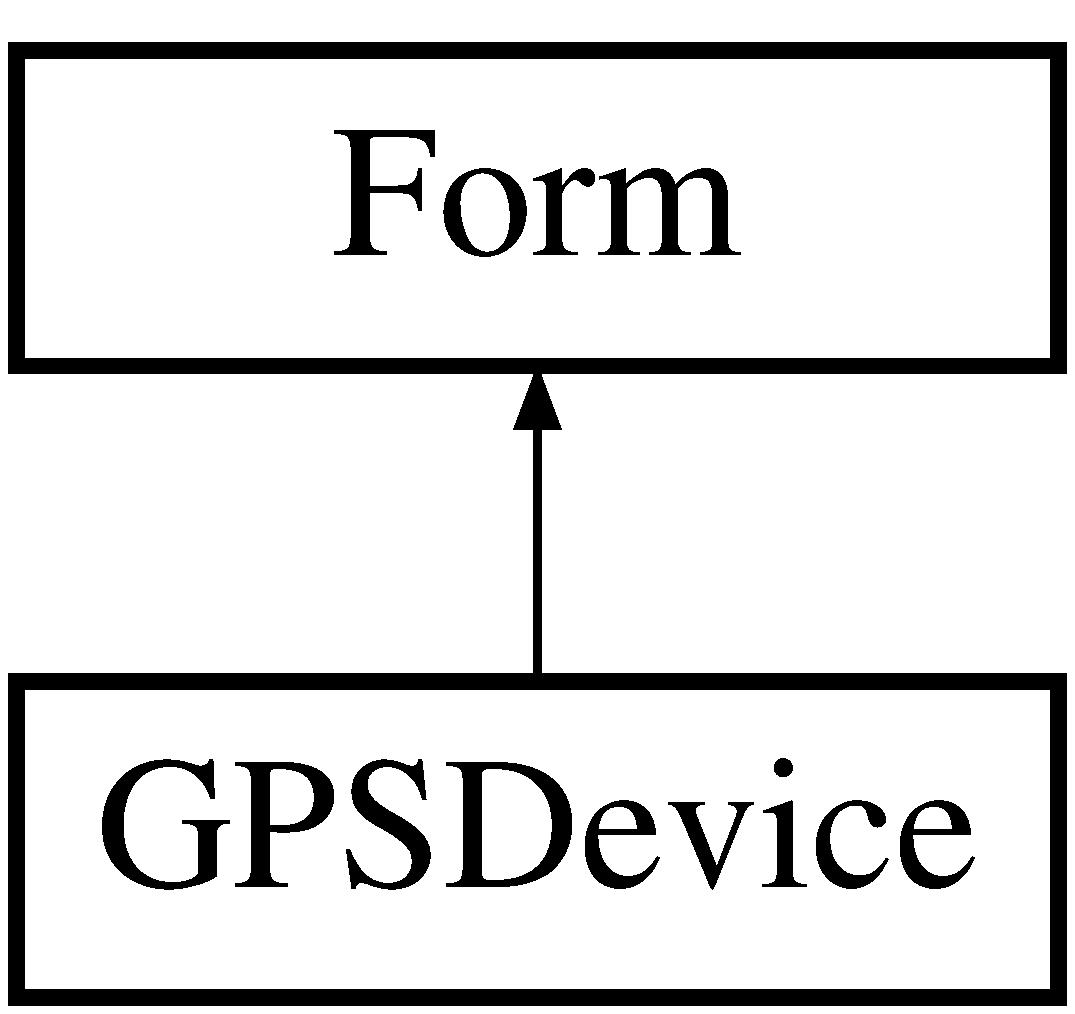
\includegraphics[height=2.000000cm]{classWildlifeTrackingApp_1_1GPSDevice}
\end{center}
\end{figure}
\subsection*{Public Member Functions}
\begin{DoxyCompactItemize}
\item 
\hyperlink{classWildlifeTrackingApp_1_1GPSDevice_a4642693badcba7273e5031b821d3656c}{G\+P\+S\+Device} ()
\end{DoxyCompactItemize}
\subsection*{Public Attributes}
\begin{DoxyCompactItemize}
\item 
int \hyperlink{classWildlifeTrackingApp_1_1GPSDevice_aad96a74a8e07bceb571a64a3355b779d}{selected\+Row}
\end{DoxyCompactItemize}
\subsection*{Protected Member Functions}
\begin{DoxyCompactItemize}
\item 
override void \hyperlink{classWildlifeTrackingApp_1_1GPSDevice_a849c3c7f8d08104f0cdb46bee9fe6389}{Dispose} (bool disposing)
\begin{DoxyCompactList}\small\item\em Clean up any resources being used. \end{DoxyCompactList}\end{DoxyCompactItemize}
\subsection*{Properties}
\begin{DoxyCompactItemize}
\item 
static log4net.\+I\+Log \hyperlink{classWildlifeTrackingApp_1_1GPSDevice_a5fc9abb86e6110ecd61d0a1a7d740a8a}{Log}\hspace{0.3cm}{\ttfamily  \mbox{[}get, private set\mbox{]}}
\end{DoxyCompactItemize}
\subsection*{Private Member Functions}
\begin{DoxyCompactItemize}
\item 
void \hyperlink{classWildlifeTrackingApp_1_1GPSDevice_ae56b21bee08f5cad9858a264ccc21fd5}{add\+\_\+button\+\_\+\+Click} (object sender, Event\+Args e)
\begin{DoxyCompactList}\small\item\em Event handler for add button click of adding new animal . \end{DoxyCompactList}\item 
void \hyperlink{classWildlifeTrackingApp_1_1GPSDevice_af87e0d54e9971bfe9ccba3a85841f619}{data\+Grid} ()
\begin{DoxyCompactList}\small\item\em It loads data to datagrid view. \end{DoxyCompactList}\item 
void \hyperlink{classWildlifeTrackingApp_1_1GPSDevice_a28f46cdb401c2c8da3f8e117eaedf977}{delete\+\_\+button\+\_\+\+Click} (object sender, Event\+Args e)
\begin{DoxyCompactList}\small\item\em Event handler for delete button click. \end{DoxyCompactList}\item 
Data\+Table \hyperlink{classWildlifeTrackingApp_1_1GPSDevice_a72673ff63cce544357c7d37b7277d2a9}{get\+All\+Animal\+List} ()
\begin{DoxyCompactList}\small\item\em Collects categroy details and saves as a datatable. \end{DoxyCompactList}\item 
\hyperlink{classWildlifeTrackingApp_1_1Models_1_1Animal}{Models.\+Animal} \hyperlink{classWildlifeTrackingApp_1_1GPSDevice_aa77ac6fe5337cfc839398bafce2995c9}{Get\+Animal\+Details} (string animal\+Name, int category\+Id, string gps\+Device\+Id)
\item 
void \hyperlink{classWildlifeTrackingApp_1_1GPSDevice_a6ea679908b776bed849fbdc9eb2e3e48}{gps\+Device\+\_\+\+Activated} (object sender, Event\+Args e)
\begin{DoxyCompactList}\small\item\em Event handler for activation of form. \end{DoxyCompactList}\item 
void \hyperlink{classWildlifeTrackingApp_1_1GPSDevice_a6405d5db675d5338663195a4d12b4c9f}{Initialize\+Component} ()
\begin{DoxyCompactList}\small\item\em Required method for Designer support -\/ do not modify the contents of this method with the code editor. \end{DoxyCompactList}\end{DoxyCompactItemize}
\subsection*{Private Attributes}
\begin{DoxyCompactItemize}
\item 
System.\+Windows.\+Forms.\+Button \hyperlink{classWildlifeTrackingApp_1_1GPSDevice_a7f1dbd5813451728f923cb88a3469cb6}{add\+\_\+button}
\item 
List$<$ \hyperlink{classWildlifeTrackingApp_1_1Models_1_1Animal}{Models.\+Animal} $>$ \hyperlink{classWildlifeTrackingApp_1_1GPSDevice_af6ea227040809ec847f3ab49aef0187c}{all\+Animals\+Located}
\item 
Data\+Table \hyperlink{classWildlifeTrackingApp_1_1GPSDevice_adb239b554c7bf520291b6165244efd42}{animal\+Details}
\item 
System.\+Component\+Model.\+I\+Container \hyperlink{classWildlifeTrackingApp_1_1GPSDevice_a02595f1c09713bb71dcb2fbbfc7ffa4b}{components} = null
\begin{DoxyCompactList}\small\item\em Required designer variable. \end{DoxyCompactList}\item 
System.\+Windows.\+Forms.\+Button \hyperlink{classWildlifeTrackingApp_1_1GPSDevice_a84dcb7863c4f709001a644ff98f22414}{delete\+\_\+button}
\item 
System.\+Windows.\+Forms.\+Data\+Grid\+View \hyperlink{classWildlifeTrackingApp_1_1GPSDevice_a39b3e0567cbf561947dccf8b8fcd9db1}{gps\+\_\+data\+Grid\+View}
\end{DoxyCompactItemize}
\subsection*{Static Private Attributes}
\begin{DoxyCompactItemize}
\item 
static readonly log4net.\+I\+Log \hyperlink{classWildlifeTrackingApp_1_1GPSDevice_ae6c6142b8525b2f4ac6ee6e003b3106f}{log}
\end{DoxyCompactItemize}


\subsection{Detailed Description}
Form class that adds loads the list of new animals , add animal ,delete animal and edit animal. 



\subsection{Constructor \& Destructor Documentation}
\mbox{\Hypertarget{classWildlifeTrackingApp_1_1GPSDevice_a4642693badcba7273e5031b821d3656c}\label{classWildlifeTrackingApp_1_1GPSDevice_a4642693badcba7273e5031b821d3656c}} 
\index{Wildlife\+Tracking\+App\+::\+G\+P\+S\+Device@{Wildlife\+Tracking\+App\+::\+G\+P\+S\+Device}!G\+P\+S\+Device@{G\+P\+S\+Device}}
\index{G\+P\+S\+Device@{G\+P\+S\+Device}!Wildlife\+Tracking\+App\+::\+G\+P\+S\+Device@{Wildlife\+Tracking\+App\+::\+G\+P\+S\+Device}}
\subsubsection{\texorpdfstring{G\+P\+S\+Device()}{GPSDevice()}}
{\footnotesize\ttfamily \hyperlink{classWildlifeTrackingApp_1_1GPSDevice}{G\+P\+S\+Device} (\begin{DoxyParamCaption}{ }\end{DoxyParamCaption})\hspace{0.3cm}{\ttfamily [inline]}}



\subsection{Member Function Documentation}
\mbox{\Hypertarget{classWildlifeTrackingApp_1_1GPSDevice_ae56b21bee08f5cad9858a264ccc21fd5}\label{classWildlifeTrackingApp_1_1GPSDevice_ae56b21bee08f5cad9858a264ccc21fd5}} 
\index{Wildlife\+Tracking\+App\+::\+G\+P\+S\+Device@{Wildlife\+Tracking\+App\+::\+G\+P\+S\+Device}!add\+\_\+button\+\_\+\+Click@{add\+\_\+button\+\_\+\+Click}}
\index{add\+\_\+button\+\_\+\+Click@{add\+\_\+button\+\_\+\+Click}!Wildlife\+Tracking\+App\+::\+G\+P\+S\+Device@{Wildlife\+Tracking\+App\+::\+G\+P\+S\+Device}}
\subsubsection{\texorpdfstring{add\+\_\+button\+\_\+\+Click()}{add\_button\_Click()}}
{\footnotesize\ttfamily void add\+\_\+button\+\_\+\+Click (\begin{DoxyParamCaption}\item[{object}]{sender,  }\item[{Event\+Args}]{e }\end{DoxyParamCaption})\hspace{0.3cm}{\ttfamily [inline]}, {\ttfamily [private]}}



Event handler for add button click of adding new animal . 


\begin{DoxyParams}{Parameters}
{\em sender} & \\
\hline
{\em e} & \\
\hline
\end{DoxyParams}
\mbox{\Hypertarget{classWildlifeTrackingApp_1_1GPSDevice_af87e0d54e9971bfe9ccba3a85841f619}\label{classWildlifeTrackingApp_1_1GPSDevice_af87e0d54e9971bfe9ccba3a85841f619}} 
\index{Wildlife\+Tracking\+App\+::\+G\+P\+S\+Device@{Wildlife\+Tracking\+App\+::\+G\+P\+S\+Device}!data\+Grid@{data\+Grid}}
\index{data\+Grid@{data\+Grid}!Wildlife\+Tracking\+App\+::\+G\+P\+S\+Device@{Wildlife\+Tracking\+App\+::\+G\+P\+S\+Device}}
\subsubsection{\texorpdfstring{data\+Grid()}{dataGrid()}}
{\footnotesize\ttfamily void data\+Grid (\begin{DoxyParamCaption}{ }\end{DoxyParamCaption})\hspace{0.3cm}{\ttfamily [inline]}, {\ttfamily [private]}}



It loads data to datagrid view. 

\mbox{\Hypertarget{classWildlifeTrackingApp_1_1GPSDevice_a28f46cdb401c2c8da3f8e117eaedf977}\label{classWildlifeTrackingApp_1_1GPSDevice_a28f46cdb401c2c8da3f8e117eaedf977}} 
\index{Wildlife\+Tracking\+App\+::\+G\+P\+S\+Device@{Wildlife\+Tracking\+App\+::\+G\+P\+S\+Device}!delete\+\_\+button\+\_\+\+Click@{delete\+\_\+button\+\_\+\+Click}}
\index{delete\+\_\+button\+\_\+\+Click@{delete\+\_\+button\+\_\+\+Click}!Wildlife\+Tracking\+App\+::\+G\+P\+S\+Device@{Wildlife\+Tracking\+App\+::\+G\+P\+S\+Device}}
\subsubsection{\texorpdfstring{delete\+\_\+button\+\_\+\+Click()}{delete\_button\_Click()}}
{\footnotesize\ttfamily void delete\+\_\+button\+\_\+\+Click (\begin{DoxyParamCaption}\item[{object}]{sender,  }\item[{Event\+Args}]{e }\end{DoxyParamCaption})\hspace{0.3cm}{\ttfamily [inline]}, {\ttfamily [private]}}



Event handler for delete button click. 


\begin{DoxyParams}{Parameters}
{\em sender} & Sender Object\\
\hline
{\em e} & Event argument\\
\hline
\end{DoxyParams}
\mbox{\Hypertarget{classWildlifeTrackingApp_1_1GPSDevice_a849c3c7f8d08104f0cdb46bee9fe6389}\label{classWildlifeTrackingApp_1_1GPSDevice_a849c3c7f8d08104f0cdb46bee9fe6389}} 
\index{Wildlife\+Tracking\+App\+::\+G\+P\+S\+Device@{Wildlife\+Tracking\+App\+::\+G\+P\+S\+Device}!Dispose@{Dispose}}
\index{Dispose@{Dispose}!Wildlife\+Tracking\+App\+::\+G\+P\+S\+Device@{Wildlife\+Tracking\+App\+::\+G\+P\+S\+Device}}
\subsubsection{\texorpdfstring{Dispose()}{Dispose()}}
{\footnotesize\ttfamily override void Dispose (\begin{DoxyParamCaption}\item[{bool}]{disposing }\end{DoxyParamCaption})\hspace{0.3cm}{\ttfamily [inline]}, {\ttfamily [protected]}}



Clean up any resources being used. 


\begin{DoxyParams}{Parameters}
{\em disposing} & true if managed resources should be disposed; otherwise, false.\\
\hline
\end{DoxyParams}
\mbox{\Hypertarget{classWildlifeTrackingApp_1_1GPSDevice_a72673ff63cce544357c7d37b7277d2a9}\label{classWildlifeTrackingApp_1_1GPSDevice_a72673ff63cce544357c7d37b7277d2a9}} 
\index{Wildlife\+Tracking\+App\+::\+G\+P\+S\+Device@{Wildlife\+Tracking\+App\+::\+G\+P\+S\+Device}!get\+All\+Animal\+List@{get\+All\+Animal\+List}}
\index{get\+All\+Animal\+List@{get\+All\+Animal\+List}!Wildlife\+Tracking\+App\+::\+G\+P\+S\+Device@{Wildlife\+Tracking\+App\+::\+G\+P\+S\+Device}}
\subsubsection{\texorpdfstring{get\+All\+Animal\+List()}{getAllAnimalList()}}
{\footnotesize\ttfamily Data\+Table get\+All\+Animal\+List (\begin{DoxyParamCaption}{ }\end{DoxyParamCaption})\hspace{0.3cm}{\ttfamily [inline]}, {\ttfamily [private]}}



Collects categroy details and saves as a datatable. 

\begin{DoxyReturn}{Returns}
Returns category data as datatable
\end{DoxyReturn}
\mbox{\Hypertarget{classWildlifeTrackingApp_1_1GPSDevice_aa77ac6fe5337cfc839398bafce2995c9}\label{classWildlifeTrackingApp_1_1GPSDevice_aa77ac6fe5337cfc839398bafce2995c9}} 
\index{Wildlife\+Tracking\+App\+::\+G\+P\+S\+Device@{Wildlife\+Tracking\+App\+::\+G\+P\+S\+Device}!Get\+Animal\+Details@{Get\+Animal\+Details}}
\index{Get\+Animal\+Details@{Get\+Animal\+Details}!Wildlife\+Tracking\+App\+::\+G\+P\+S\+Device@{Wildlife\+Tracking\+App\+::\+G\+P\+S\+Device}}
\subsubsection{\texorpdfstring{Get\+Animal\+Details()}{GetAnimalDetails()}}
{\footnotesize\ttfamily \hyperlink{classWildlifeTrackingApp_1_1Models_1_1Animal}{Models.\+Animal} Get\+Animal\+Details (\begin{DoxyParamCaption}\item[{string}]{animal\+Name,  }\item[{int}]{category\+Id,  }\item[{string}]{gps\+Device\+Id }\end{DoxyParamCaption})\hspace{0.3cm}{\ttfamily [inline]}, {\ttfamily [private]}}

\mbox{\Hypertarget{classWildlifeTrackingApp_1_1GPSDevice_a6ea679908b776bed849fbdc9eb2e3e48}\label{classWildlifeTrackingApp_1_1GPSDevice_a6ea679908b776bed849fbdc9eb2e3e48}} 
\index{Wildlife\+Tracking\+App\+::\+G\+P\+S\+Device@{Wildlife\+Tracking\+App\+::\+G\+P\+S\+Device}!gps\+Device\+\_\+\+Activated@{gps\+Device\+\_\+\+Activated}}
\index{gps\+Device\+\_\+\+Activated@{gps\+Device\+\_\+\+Activated}!Wildlife\+Tracking\+App\+::\+G\+P\+S\+Device@{Wildlife\+Tracking\+App\+::\+G\+P\+S\+Device}}
\subsubsection{\texorpdfstring{gps\+Device\+\_\+\+Activated()}{gpsDevice\_Activated()}}
{\footnotesize\ttfamily void gps\+Device\+\_\+\+Activated (\begin{DoxyParamCaption}\item[{object}]{sender,  }\item[{Event\+Args}]{e }\end{DoxyParamCaption})\hspace{0.3cm}{\ttfamily [inline]}, {\ttfamily [private]}}



Event handler for activation of form. 


\begin{DoxyParams}{Parameters}
{\em sender} & Sender Object\\
\hline
{\em e} & Event Argument\\
\hline
\end{DoxyParams}
\mbox{\Hypertarget{classWildlifeTrackingApp_1_1GPSDevice_a6405d5db675d5338663195a4d12b4c9f}\label{classWildlifeTrackingApp_1_1GPSDevice_a6405d5db675d5338663195a4d12b4c9f}} 
\index{Wildlife\+Tracking\+App\+::\+G\+P\+S\+Device@{Wildlife\+Tracking\+App\+::\+G\+P\+S\+Device}!Initialize\+Component@{Initialize\+Component}}
\index{Initialize\+Component@{Initialize\+Component}!Wildlife\+Tracking\+App\+::\+G\+P\+S\+Device@{Wildlife\+Tracking\+App\+::\+G\+P\+S\+Device}}
\subsubsection{\texorpdfstring{Initialize\+Component()}{InitializeComponent()}}
{\footnotesize\ttfamily void Initialize\+Component (\begin{DoxyParamCaption}{ }\end{DoxyParamCaption})\hspace{0.3cm}{\ttfamily [inline]}, {\ttfamily [private]}}



Required method for Designer support -\/ do not modify the contents of this method with the code editor. 



\subsection{Member Data Documentation}
\mbox{\Hypertarget{classWildlifeTrackingApp_1_1GPSDevice_a7f1dbd5813451728f923cb88a3469cb6}\label{classWildlifeTrackingApp_1_1GPSDevice_a7f1dbd5813451728f923cb88a3469cb6}} 
\index{Wildlife\+Tracking\+App\+::\+G\+P\+S\+Device@{Wildlife\+Tracking\+App\+::\+G\+P\+S\+Device}!add\+\_\+button@{add\+\_\+button}}
\index{add\+\_\+button@{add\+\_\+button}!Wildlife\+Tracking\+App\+::\+G\+P\+S\+Device@{Wildlife\+Tracking\+App\+::\+G\+P\+S\+Device}}
\subsubsection{\texorpdfstring{add\+\_\+button}{add\_button}}
{\footnotesize\ttfamily System.\+Windows.\+Forms.\+Button add\+\_\+button\hspace{0.3cm}{\ttfamily [private]}}

\mbox{\Hypertarget{classWildlifeTrackingApp_1_1GPSDevice_af6ea227040809ec847f3ab49aef0187c}\label{classWildlifeTrackingApp_1_1GPSDevice_af6ea227040809ec847f3ab49aef0187c}} 
\index{Wildlife\+Tracking\+App\+::\+G\+P\+S\+Device@{Wildlife\+Tracking\+App\+::\+G\+P\+S\+Device}!all\+Animals\+Located@{all\+Animals\+Located}}
\index{all\+Animals\+Located@{all\+Animals\+Located}!Wildlife\+Tracking\+App\+::\+G\+P\+S\+Device@{Wildlife\+Tracking\+App\+::\+G\+P\+S\+Device}}
\subsubsection{\texorpdfstring{all\+Animals\+Located}{allAnimalsLocated}}
{\footnotesize\ttfamily List$<$\hyperlink{classWildlifeTrackingApp_1_1Models_1_1Animal}{Models.\+Animal}$>$ all\+Animals\+Located\hspace{0.3cm}{\ttfamily [private]}}

\mbox{\Hypertarget{classWildlifeTrackingApp_1_1GPSDevice_adb239b554c7bf520291b6165244efd42}\label{classWildlifeTrackingApp_1_1GPSDevice_adb239b554c7bf520291b6165244efd42}} 
\index{Wildlife\+Tracking\+App\+::\+G\+P\+S\+Device@{Wildlife\+Tracking\+App\+::\+G\+P\+S\+Device}!animal\+Details@{animal\+Details}}
\index{animal\+Details@{animal\+Details}!Wildlife\+Tracking\+App\+::\+G\+P\+S\+Device@{Wildlife\+Tracking\+App\+::\+G\+P\+S\+Device}}
\subsubsection{\texorpdfstring{animal\+Details}{animalDetails}}
{\footnotesize\ttfamily Data\+Table animal\+Details\hspace{0.3cm}{\ttfamily [private]}}

\mbox{\Hypertarget{classWildlifeTrackingApp_1_1GPSDevice_a02595f1c09713bb71dcb2fbbfc7ffa4b}\label{classWildlifeTrackingApp_1_1GPSDevice_a02595f1c09713bb71dcb2fbbfc7ffa4b}} 
\index{Wildlife\+Tracking\+App\+::\+G\+P\+S\+Device@{Wildlife\+Tracking\+App\+::\+G\+P\+S\+Device}!components@{components}}
\index{components@{components}!Wildlife\+Tracking\+App\+::\+G\+P\+S\+Device@{Wildlife\+Tracking\+App\+::\+G\+P\+S\+Device}}
\subsubsection{\texorpdfstring{components}{components}}
{\footnotesize\ttfamily System.\+Component\+Model.\+I\+Container components = null\hspace{0.3cm}{\ttfamily [private]}}



Required designer variable. 

\mbox{\Hypertarget{classWildlifeTrackingApp_1_1GPSDevice_a84dcb7863c4f709001a644ff98f22414}\label{classWildlifeTrackingApp_1_1GPSDevice_a84dcb7863c4f709001a644ff98f22414}} 
\index{Wildlife\+Tracking\+App\+::\+G\+P\+S\+Device@{Wildlife\+Tracking\+App\+::\+G\+P\+S\+Device}!delete\+\_\+button@{delete\+\_\+button}}
\index{delete\+\_\+button@{delete\+\_\+button}!Wildlife\+Tracking\+App\+::\+G\+P\+S\+Device@{Wildlife\+Tracking\+App\+::\+G\+P\+S\+Device}}
\subsubsection{\texorpdfstring{delete\+\_\+button}{delete\_button}}
{\footnotesize\ttfamily System.\+Windows.\+Forms.\+Button delete\+\_\+button\hspace{0.3cm}{\ttfamily [private]}}

\mbox{\Hypertarget{classWildlifeTrackingApp_1_1GPSDevice_a39b3e0567cbf561947dccf8b8fcd9db1}\label{classWildlifeTrackingApp_1_1GPSDevice_a39b3e0567cbf561947dccf8b8fcd9db1}} 
\index{Wildlife\+Tracking\+App\+::\+G\+P\+S\+Device@{Wildlife\+Tracking\+App\+::\+G\+P\+S\+Device}!gps\+\_\+data\+Grid\+View@{gps\+\_\+data\+Grid\+View}}
\index{gps\+\_\+data\+Grid\+View@{gps\+\_\+data\+Grid\+View}!Wildlife\+Tracking\+App\+::\+G\+P\+S\+Device@{Wildlife\+Tracking\+App\+::\+G\+P\+S\+Device}}
\subsubsection{\texorpdfstring{gps\+\_\+data\+Grid\+View}{gps\_dataGridView}}
{\footnotesize\ttfamily System.\+Windows.\+Forms.\+Data\+Grid\+View gps\+\_\+data\+Grid\+View\hspace{0.3cm}{\ttfamily [private]}}

\mbox{\Hypertarget{classWildlifeTrackingApp_1_1GPSDevice_ae6c6142b8525b2f4ac6ee6e003b3106f}\label{classWildlifeTrackingApp_1_1GPSDevice_ae6c6142b8525b2f4ac6ee6e003b3106f}} 
\index{Wildlife\+Tracking\+App\+::\+G\+P\+S\+Device@{Wildlife\+Tracking\+App\+::\+G\+P\+S\+Device}!log@{log}}
\index{log@{log}!Wildlife\+Tracking\+App\+::\+G\+P\+S\+Device@{Wildlife\+Tracking\+App\+::\+G\+P\+S\+Device}}
\subsubsection{\texorpdfstring{log}{log}}
{\footnotesize\ttfamily readonly log4net.\+I\+Log log\hspace{0.3cm}{\ttfamily [static]}, {\ttfamily [private]}}

{\bfseries Initial value\+:}
\begin{DoxyCode}
= log4net.LogManager.GetLogger
        (\hyperlink{namespaceSystem}{System}.Reflection.MethodBase.GetCurrentMethod().DeclaringType)
\end{DoxyCode}
\mbox{\Hypertarget{classWildlifeTrackingApp_1_1GPSDevice_aad96a74a8e07bceb571a64a3355b779d}\label{classWildlifeTrackingApp_1_1GPSDevice_aad96a74a8e07bceb571a64a3355b779d}} 
\index{Wildlife\+Tracking\+App\+::\+G\+P\+S\+Device@{Wildlife\+Tracking\+App\+::\+G\+P\+S\+Device}!selected\+Row@{selected\+Row}}
\index{selected\+Row@{selected\+Row}!Wildlife\+Tracking\+App\+::\+G\+P\+S\+Device@{Wildlife\+Tracking\+App\+::\+G\+P\+S\+Device}}
\subsubsection{\texorpdfstring{selected\+Row}{selectedRow}}
{\footnotesize\ttfamily int selected\+Row}



\subsection{Property Documentation}
\mbox{\Hypertarget{classWildlifeTrackingApp_1_1GPSDevice_a5fc9abb86e6110ecd61d0a1a7d740a8a}\label{classWildlifeTrackingApp_1_1GPSDevice_a5fc9abb86e6110ecd61d0a1a7d740a8a}} 
\index{Wildlife\+Tracking\+App\+::\+G\+P\+S\+Device@{Wildlife\+Tracking\+App\+::\+G\+P\+S\+Device}!Log@{Log}}
\index{Log@{Log}!Wildlife\+Tracking\+App\+::\+G\+P\+S\+Device@{Wildlife\+Tracking\+App\+::\+G\+P\+S\+Device}}
\subsubsection{\texorpdfstring{Log}{Log}}
{\footnotesize\ttfamily log4net.\+I\+Log Log\hspace{0.3cm}{\ttfamily [static]}, {\ttfamily [get]}, {\ttfamily [private set]}}



The documentation for this class was generated from the following files\+:\begin{DoxyCompactItemize}
\item 
View/\hyperlink{GPSDevice_8cs}{G\+P\+S\+Device.\+cs}\item 
View/\hyperlink{GPSDevice_8Designer_8cs}{G\+P\+S\+Device.\+Designer.\+cs}\end{DoxyCompactItemize}

\hypertarget{classWildlifeTrackingApp_1_1LocateCategory}{}\section{Locate\+Category}
\label{classWildlifeTrackingApp_1_1LocateCategory}\index{Locate\+Category@{Locate\+Category}}


Form class that loads map and locates the animals from given categories.  


Inheritance diagram for Locate\+Category\+:\begin{figure}[H]
\begin{center}
\leavevmode
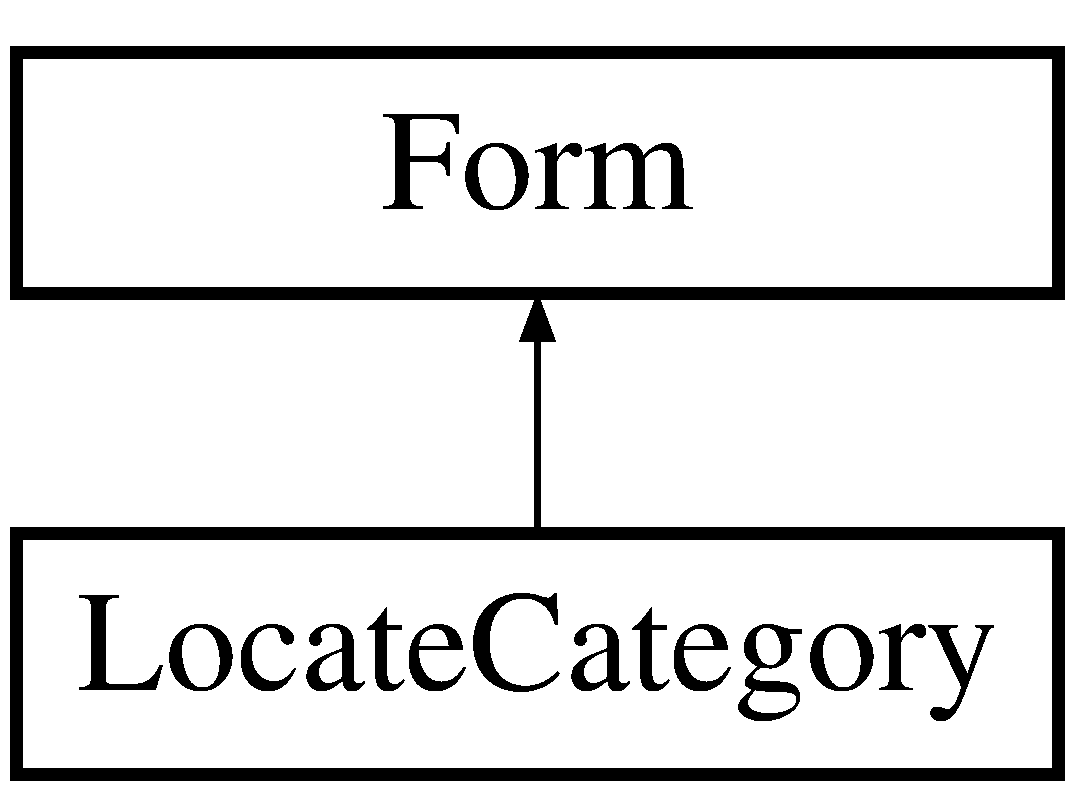
\includegraphics[height=2.000000cm]{classWildlifeTrackingApp_1_1LocateCategory}
\end{center}
\end{figure}
\subsection*{Public Member Functions}
\begin{DoxyCompactItemize}
\item 
\hyperlink{classWildlifeTrackingApp_1_1LocateCategory_abdc0fce16d0e2de3af4c81225ae3c925}{Locate\+Category} ()
\end{DoxyCompactItemize}
\subsection*{Protected Member Functions}
\begin{DoxyCompactItemize}
\item 
override void \hyperlink{classWildlifeTrackingApp_1_1LocateCategory_a849c3c7f8d08104f0cdb46bee9fe6389}{Dispose} (bool disposing)
\begin{DoxyCompactList}\small\item\em Clean up any resources being used. \end{DoxyCompactList}\end{DoxyCompactItemize}
\subsection*{Properties}
\begin{DoxyCompactItemize}
\item 
static log4net.\+I\+Log \hyperlink{classWildlifeTrackingApp_1_1LocateCategory_a5fc9abb86e6110ecd61d0a1a7d740a8a}{Log}\hspace{0.3cm}{\ttfamily  \mbox{[}get, private set\mbox{]}}
\end{DoxyCompactItemize}
\subsection*{Private Member Functions}
\begin{DoxyCompactItemize}
\item 
void \hyperlink{classWildlifeTrackingApp_1_1LocateCategory_a99a28fbc72be710413039cec9aeeba10}{configure\+Zooming\+Of\+Map} ()
\item 
void \hyperlink{classWildlifeTrackingApp_1_1LocateCategory_a7f17e416fe1ed8e8eba93a84a5aecb11}{g\+Map\+Control\+\_\+\+Load} (object sender, Event\+Args e)
\begin{DoxyCompactList}\small\item\em Loads the Gmap. \end{DoxyCompactList}\item 
void \hyperlink{classWildlifeTrackingApp_1_1LocateCategory_a6405d5db675d5338663195a4d12b4c9f}{Initialize\+Component} ()
\begin{DoxyCompactList}\small\item\em Required method for Designer support -\/ do not modify the contents of this method with the code editor. \end{DoxyCompactList}\item 
void \hyperlink{classWildlifeTrackingApp_1_1LocateCategory_a4556db306d6b4b0b473df21ef87398c5}{load\+Google\+Map\+For\+All\+Category} ()
\begin{DoxyCompactList}\small\item\em Locates total animals from all categoreies in Gmap. \end{DoxyCompactList}\item 
void \hyperlink{classWildlifeTrackingApp_1_1LocateCategory_a9b1d54086f1fa768d30c15fdc1971924}{load\+Google\+Map\+Per\+Category} ()
\begin{DoxyCompactList}\small\item\em Locates animals from the selected category. \end{DoxyCompactList}\item 
void \hyperlink{classWildlifeTrackingApp_1_1LocateCategory_ab9a46ca8e764049be2d465a144610180}{locate\+Category\+\_\+\+Activated} (object sender, Event\+Args e)
\begin{DoxyCompactList}\small\item\em Event handler for the activation of the form. \end{DoxyCompactList}\item 
void \hyperlink{classWildlifeTrackingApp_1_1LocateCategory_a613e5c1a6893ab25486d97ab4e17d7e8}{locate\+Selected\+Category} (object sender, Event\+Args e)
\begin{DoxyCompactList}\small\item\em Event handler for the selection change of drop down menu. It locates the all animals from a particular categories or from all categories choosen based on drop down menu selection. \end{DoxyCompactList}\end{DoxyCompactItemize}
\subsection*{Private Attributes}
\begin{DoxyCompactItemize}
\item 
System.\+Windows.\+Forms.\+Combo\+Box \hyperlink{classWildlifeTrackingApp_1_1LocateCategory_a8b1f399ade6c575e8562bc7d574d60d5}{category\+\_\+combo\+Box}
\item 
System.\+Windows.\+Forms.\+Label \hyperlink{classWildlifeTrackingApp_1_1LocateCategory_ad2144d281f164c5692cabbdd67e60c00}{category\+Name\+\_\+label}
\item 
System.\+Component\+Model.\+I\+Container \hyperlink{classWildlifeTrackingApp_1_1LocateCategory_a02595f1c09713bb71dcb2fbbfc7ffa4b}{components} = null
\begin{DoxyCompactList}\small\item\em Required designer variable. \end{DoxyCompactList}\item 
G\+Map.\+N\+E\+T.\+Windows\+Forms.\+G\+Map\+Control \hyperlink{classWildlifeTrackingApp_1_1LocateCategory_a33b985f58f15052a572266a4a0b43637}{g\+Map\+Control}
\item 
System.\+Windows.\+Forms.\+Label \hyperlink{classWildlifeTrackingApp_1_1LocateCategory_a2fd4190abaec4ee146747d5a024d1bda}{select\+Category\+\_\+label}
\end{DoxyCompactItemize}
\subsection*{Static Private Attributes}
\begin{DoxyCompactItemize}
\item 
static readonly log4net.\+I\+Log \hyperlink{classWildlifeTrackingApp_1_1LocateCategory_ae6c6142b8525b2f4ac6ee6e003b3106f}{log}
\end{DoxyCompactItemize}


\subsection{Detailed Description}
Form class that loads map and locates the animals from given categories. 



\subsection{Constructor \& Destructor Documentation}
\mbox{\Hypertarget{classWildlifeTrackingApp_1_1LocateCategory_abdc0fce16d0e2de3af4c81225ae3c925}\label{classWildlifeTrackingApp_1_1LocateCategory_abdc0fce16d0e2de3af4c81225ae3c925}} 
\index{Wildlife\+Tracking\+App\+::\+Locate\+Category@{Wildlife\+Tracking\+App\+::\+Locate\+Category}!Locate\+Category@{Locate\+Category}}
\index{Locate\+Category@{Locate\+Category}!Wildlife\+Tracking\+App\+::\+Locate\+Category@{Wildlife\+Tracking\+App\+::\+Locate\+Category}}
\subsubsection{\texorpdfstring{Locate\+Category()}{LocateCategory()}}
{\footnotesize\ttfamily \hyperlink{classWildlifeTrackingApp_1_1LocateCategory}{Locate\+Category} (\begin{DoxyParamCaption}{ }\end{DoxyParamCaption})\hspace{0.3cm}{\ttfamily [inline]}}



\subsection{Member Function Documentation}
\mbox{\Hypertarget{classWildlifeTrackingApp_1_1LocateCategory_a99a28fbc72be710413039cec9aeeba10}\label{classWildlifeTrackingApp_1_1LocateCategory_a99a28fbc72be710413039cec9aeeba10}} 
\index{Wildlife\+Tracking\+App\+::\+Locate\+Category@{Wildlife\+Tracking\+App\+::\+Locate\+Category}!configure\+Zooming\+Of\+Map@{configure\+Zooming\+Of\+Map}}
\index{configure\+Zooming\+Of\+Map@{configure\+Zooming\+Of\+Map}!Wildlife\+Tracking\+App\+::\+Locate\+Category@{Wildlife\+Tracking\+App\+::\+Locate\+Category}}
\subsubsection{\texorpdfstring{configure\+Zooming\+Of\+Map()}{configureZoomingOfMap()}}
{\footnotesize\ttfamily void configure\+Zooming\+Of\+Map (\begin{DoxyParamCaption}{ }\end{DoxyParamCaption})\hspace{0.3cm}{\ttfamily [inline]}, {\ttfamily [private]}}

\mbox{\Hypertarget{classWildlifeTrackingApp_1_1LocateCategory_a849c3c7f8d08104f0cdb46bee9fe6389}\label{classWildlifeTrackingApp_1_1LocateCategory_a849c3c7f8d08104f0cdb46bee9fe6389}} 
\index{Wildlife\+Tracking\+App\+::\+Locate\+Category@{Wildlife\+Tracking\+App\+::\+Locate\+Category}!Dispose@{Dispose}}
\index{Dispose@{Dispose}!Wildlife\+Tracking\+App\+::\+Locate\+Category@{Wildlife\+Tracking\+App\+::\+Locate\+Category}}
\subsubsection{\texorpdfstring{Dispose()}{Dispose()}}
{\footnotesize\ttfamily override void Dispose (\begin{DoxyParamCaption}\item[{bool}]{disposing }\end{DoxyParamCaption})\hspace{0.3cm}{\ttfamily [inline]}, {\ttfamily [protected]}}



Clean up any resources being used. 


\begin{DoxyParams}{Parameters}
{\em disposing} & true if managed resources should be disposed; otherwise, false.\\
\hline
\end{DoxyParams}
\mbox{\Hypertarget{classWildlifeTrackingApp_1_1LocateCategory_a7f17e416fe1ed8e8eba93a84a5aecb11}\label{classWildlifeTrackingApp_1_1LocateCategory_a7f17e416fe1ed8e8eba93a84a5aecb11}} 
\index{Wildlife\+Tracking\+App\+::\+Locate\+Category@{Wildlife\+Tracking\+App\+::\+Locate\+Category}!g\+Map\+Control\+\_\+\+Load@{g\+Map\+Control\+\_\+\+Load}}
\index{g\+Map\+Control\+\_\+\+Load@{g\+Map\+Control\+\_\+\+Load}!Wildlife\+Tracking\+App\+::\+Locate\+Category@{Wildlife\+Tracking\+App\+::\+Locate\+Category}}
\subsubsection{\texorpdfstring{g\+Map\+Control\+\_\+\+Load()}{gMapControl\_Load()}}
{\footnotesize\ttfamily void g\+Map\+Control\+\_\+\+Load (\begin{DoxyParamCaption}\item[{object}]{sender,  }\item[{Event\+Args}]{e }\end{DoxyParamCaption})\hspace{0.3cm}{\ttfamily [inline]}, {\ttfamily [private]}}



Loads the Gmap. 


\begin{DoxyParams}{Parameters}
{\em sender} & Sender Object\\
\hline
{\em e} & Event argument\\
\hline
\end{DoxyParams}
\mbox{\Hypertarget{classWildlifeTrackingApp_1_1LocateCategory_a6405d5db675d5338663195a4d12b4c9f}\label{classWildlifeTrackingApp_1_1LocateCategory_a6405d5db675d5338663195a4d12b4c9f}} 
\index{Wildlife\+Tracking\+App\+::\+Locate\+Category@{Wildlife\+Tracking\+App\+::\+Locate\+Category}!Initialize\+Component@{Initialize\+Component}}
\index{Initialize\+Component@{Initialize\+Component}!Wildlife\+Tracking\+App\+::\+Locate\+Category@{Wildlife\+Tracking\+App\+::\+Locate\+Category}}
\subsubsection{\texorpdfstring{Initialize\+Component()}{InitializeComponent()}}
{\footnotesize\ttfamily void Initialize\+Component (\begin{DoxyParamCaption}{ }\end{DoxyParamCaption})\hspace{0.3cm}{\ttfamily [inline]}, {\ttfamily [private]}}



Required method for Designer support -\/ do not modify the contents of this method with the code editor. 

\mbox{\Hypertarget{classWildlifeTrackingApp_1_1LocateCategory_a4556db306d6b4b0b473df21ef87398c5}\label{classWildlifeTrackingApp_1_1LocateCategory_a4556db306d6b4b0b473df21ef87398c5}} 
\index{Wildlife\+Tracking\+App\+::\+Locate\+Category@{Wildlife\+Tracking\+App\+::\+Locate\+Category}!load\+Google\+Map\+For\+All\+Category@{load\+Google\+Map\+For\+All\+Category}}
\index{load\+Google\+Map\+For\+All\+Category@{load\+Google\+Map\+For\+All\+Category}!Wildlife\+Tracking\+App\+::\+Locate\+Category@{Wildlife\+Tracking\+App\+::\+Locate\+Category}}
\subsubsection{\texorpdfstring{load\+Google\+Map\+For\+All\+Category()}{loadGoogleMapForAllCategory()}}
{\footnotesize\ttfamily void load\+Google\+Map\+For\+All\+Category (\begin{DoxyParamCaption}{ }\end{DoxyParamCaption})\hspace{0.3cm}{\ttfamily [inline]}, {\ttfamily [private]}}



Locates total animals from all categoreies in Gmap. 

\mbox{\Hypertarget{classWildlifeTrackingApp_1_1LocateCategory_a9b1d54086f1fa768d30c15fdc1971924}\label{classWildlifeTrackingApp_1_1LocateCategory_a9b1d54086f1fa768d30c15fdc1971924}} 
\index{Wildlife\+Tracking\+App\+::\+Locate\+Category@{Wildlife\+Tracking\+App\+::\+Locate\+Category}!load\+Google\+Map\+Per\+Category@{load\+Google\+Map\+Per\+Category}}
\index{load\+Google\+Map\+Per\+Category@{load\+Google\+Map\+Per\+Category}!Wildlife\+Tracking\+App\+::\+Locate\+Category@{Wildlife\+Tracking\+App\+::\+Locate\+Category}}
\subsubsection{\texorpdfstring{load\+Google\+Map\+Per\+Category()}{loadGoogleMapPerCategory()}}
{\footnotesize\ttfamily void load\+Google\+Map\+Per\+Category (\begin{DoxyParamCaption}{ }\end{DoxyParamCaption})\hspace{0.3cm}{\ttfamily [inline]}, {\ttfamily [private]}}



Locates animals from the selected category. 

\mbox{\Hypertarget{classWildlifeTrackingApp_1_1LocateCategory_ab9a46ca8e764049be2d465a144610180}\label{classWildlifeTrackingApp_1_1LocateCategory_ab9a46ca8e764049be2d465a144610180}} 
\index{Wildlife\+Tracking\+App\+::\+Locate\+Category@{Wildlife\+Tracking\+App\+::\+Locate\+Category}!locate\+Category\+\_\+\+Activated@{locate\+Category\+\_\+\+Activated}}
\index{locate\+Category\+\_\+\+Activated@{locate\+Category\+\_\+\+Activated}!Wildlife\+Tracking\+App\+::\+Locate\+Category@{Wildlife\+Tracking\+App\+::\+Locate\+Category}}
\subsubsection{\texorpdfstring{locate\+Category\+\_\+\+Activated()}{locateCategory\_Activated()}}
{\footnotesize\ttfamily void locate\+Category\+\_\+\+Activated (\begin{DoxyParamCaption}\item[{object}]{sender,  }\item[{Event\+Args}]{e }\end{DoxyParamCaption})\hspace{0.3cm}{\ttfamily [inline]}, {\ttfamily [private]}}



Event handler for the activation of the form. 


\begin{DoxyParams}{Parameters}
{\em sender} & Sender Object\\
\hline
{\em e} & Event argument\\
\hline
\end{DoxyParams}
\mbox{\Hypertarget{classWildlifeTrackingApp_1_1LocateCategory_a613e5c1a6893ab25486d97ab4e17d7e8}\label{classWildlifeTrackingApp_1_1LocateCategory_a613e5c1a6893ab25486d97ab4e17d7e8}} 
\index{Wildlife\+Tracking\+App\+::\+Locate\+Category@{Wildlife\+Tracking\+App\+::\+Locate\+Category}!locate\+Selected\+Category@{locate\+Selected\+Category}}
\index{locate\+Selected\+Category@{locate\+Selected\+Category}!Wildlife\+Tracking\+App\+::\+Locate\+Category@{Wildlife\+Tracking\+App\+::\+Locate\+Category}}
\subsubsection{\texorpdfstring{locate\+Selected\+Category()}{locateSelectedCategory()}}
{\footnotesize\ttfamily void locate\+Selected\+Category (\begin{DoxyParamCaption}\item[{object}]{sender,  }\item[{Event\+Args}]{e }\end{DoxyParamCaption})\hspace{0.3cm}{\ttfamily [inline]}, {\ttfamily [private]}}



Event handler for the selection change of drop down menu. It locates the all animals from a particular categories or from all categories choosen based on drop down menu selection. 


\begin{DoxyParams}{Parameters}
{\em sender} & Sender Object\\
\hline
{\em e} & Event argument\\
\hline
\end{DoxyParams}


\subsection{Member Data Documentation}
\mbox{\Hypertarget{classWildlifeTrackingApp_1_1LocateCategory_a8b1f399ade6c575e8562bc7d574d60d5}\label{classWildlifeTrackingApp_1_1LocateCategory_a8b1f399ade6c575e8562bc7d574d60d5}} 
\index{Wildlife\+Tracking\+App\+::\+Locate\+Category@{Wildlife\+Tracking\+App\+::\+Locate\+Category}!category\+\_\+combo\+Box@{category\+\_\+combo\+Box}}
\index{category\+\_\+combo\+Box@{category\+\_\+combo\+Box}!Wildlife\+Tracking\+App\+::\+Locate\+Category@{Wildlife\+Tracking\+App\+::\+Locate\+Category}}
\subsubsection{\texorpdfstring{category\+\_\+combo\+Box}{category\_comboBox}}
{\footnotesize\ttfamily System.\+Windows.\+Forms.\+Combo\+Box category\+\_\+combo\+Box\hspace{0.3cm}{\ttfamily [private]}}

\mbox{\Hypertarget{classWildlifeTrackingApp_1_1LocateCategory_ad2144d281f164c5692cabbdd67e60c00}\label{classWildlifeTrackingApp_1_1LocateCategory_ad2144d281f164c5692cabbdd67e60c00}} 
\index{Wildlife\+Tracking\+App\+::\+Locate\+Category@{Wildlife\+Tracking\+App\+::\+Locate\+Category}!category\+Name\+\_\+label@{category\+Name\+\_\+label}}
\index{category\+Name\+\_\+label@{category\+Name\+\_\+label}!Wildlife\+Tracking\+App\+::\+Locate\+Category@{Wildlife\+Tracking\+App\+::\+Locate\+Category}}
\subsubsection{\texorpdfstring{category\+Name\+\_\+label}{categoryName\_label}}
{\footnotesize\ttfamily System.\+Windows.\+Forms.\+Label category\+Name\+\_\+label\hspace{0.3cm}{\ttfamily [private]}}

\mbox{\Hypertarget{classWildlifeTrackingApp_1_1LocateCategory_a02595f1c09713bb71dcb2fbbfc7ffa4b}\label{classWildlifeTrackingApp_1_1LocateCategory_a02595f1c09713bb71dcb2fbbfc7ffa4b}} 
\index{Wildlife\+Tracking\+App\+::\+Locate\+Category@{Wildlife\+Tracking\+App\+::\+Locate\+Category}!components@{components}}
\index{components@{components}!Wildlife\+Tracking\+App\+::\+Locate\+Category@{Wildlife\+Tracking\+App\+::\+Locate\+Category}}
\subsubsection{\texorpdfstring{components}{components}}
{\footnotesize\ttfamily System.\+Component\+Model.\+I\+Container components = null\hspace{0.3cm}{\ttfamily [private]}}



Required designer variable. 

\mbox{\Hypertarget{classWildlifeTrackingApp_1_1LocateCategory_a33b985f58f15052a572266a4a0b43637}\label{classWildlifeTrackingApp_1_1LocateCategory_a33b985f58f15052a572266a4a0b43637}} 
\index{Wildlife\+Tracking\+App\+::\+Locate\+Category@{Wildlife\+Tracking\+App\+::\+Locate\+Category}!g\+Map\+Control@{g\+Map\+Control}}
\index{g\+Map\+Control@{g\+Map\+Control}!Wildlife\+Tracking\+App\+::\+Locate\+Category@{Wildlife\+Tracking\+App\+::\+Locate\+Category}}
\subsubsection{\texorpdfstring{g\+Map\+Control}{gMapControl}}
{\footnotesize\ttfamily G\+Map.\+N\+E\+T.\+Windows\+Forms.\+G\+Map\+Control g\+Map\+Control\hspace{0.3cm}{\ttfamily [private]}}

\mbox{\Hypertarget{classWildlifeTrackingApp_1_1LocateCategory_ae6c6142b8525b2f4ac6ee6e003b3106f}\label{classWildlifeTrackingApp_1_1LocateCategory_ae6c6142b8525b2f4ac6ee6e003b3106f}} 
\index{Wildlife\+Tracking\+App\+::\+Locate\+Category@{Wildlife\+Tracking\+App\+::\+Locate\+Category}!log@{log}}
\index{log@{log}!Wildlife\+Tracking\+App\+::\+Locate\+Category@{Wildlife\+Tracking\+App\+::\+Locate\+Category}}
\subsubsection{\texorpdfstring{log}{log}}
{\footnotesize\ttfamily readonly log4net.\+I\+Log log\hspace{0.3cm}{\ttfamily [static]}, {\ttfamily [private]}}

{\bfseries Initial value\+:}
\begin{DoxyCode}
= log4net.LogManager.GetLogger
        (\hyperlink{namespaceSystem}{System}.Reflection.MethodBase.GetCurrentMethod().DeclaringType)
\end{DoxyCode}
\mbox{\Hypertarget{classWildlifeTrackingApp_1_1LocateCategory_a2fd4190abaec4ee146747d5a024d1bda}\label{classWildlifeTrackingApp_1_1LocateCategory_a2fd4190abaec4ee146747d5a024d1bda}} 
\index{Wildlife\+Tracking\+App\+::\+Locate\+Category@{Wildlife\+Tracking\+App\+::\+Locate\+Category}!select\+Category\+\_\+label@{select\+Category\+\_\+label}}
\index{select\+Category\+\_\+label@{select\+Category\+\_\+label}!Wildlife\+Tracking\+App\+::\+Locate\+Category@{Wildlife\+Tracking\+App\+::\+Locate\+Category}}
\subsubsection{\texorpdfstring{select\+Category\+\_\+label}{selectCategory\_label}}
{\footnotesize\ttfamily System.\+Windows.\+Forms.\+Label select\+Category\+\_\+label\hspace{0.3cm}{\ttfamily [private]}}



\subsection{Property Documentation}
\mbox{\Hypertarget{classWildlifeTrackingApp_1_1LocateCategory_a5fc9abb86e6110ecd61d0a1a7d740a8a}\label{classWildlifeTrackingApp_1_1LocateCategory_a5fc9abb86e6110ecd61d0a1a7d740a8a}} 
\index{Wildlife\+Tracking\+App\+::\+Locate\+Category@{Wildlife\+Tracking\+App\+::\+Locate\+Category}!Log@{Log}}
\index{Log@{Log}!Wildlife\+Tracking\+App\+::\+Locate\+Category@{Wildlife\+Tracking\+App\+::\+Locate\+Category}}
\subsubsection{\texorpdfstring{Log}{Log}}
{\footnotesize\ttfamily log4net.\+I\+Log Log\hspace{0.3cm}{\ttfamily [static]}, {\ttfamily [get]}, {\ttfamily [private set]}}



The documentation for this class was generated from the following files\+:\begin{DoxyCompactItemize}
\item 
View/\hyperlink{LocateCategory_8cs}{Locate\+Category.\+cs}\item 
View/\hyperlink{LocateCategory_8Designer_8cs}{Locate\+Category.\+Designer.\+cs}\end{DoxyCompactItemize}

\hypertarget{classWildlifeTrackingApp_1_1MainPage}{}\section{Main\+Page}
\label{classWildlifeTrackingApp_1_1MainPage}\index{Main\+Page@{Main\+Page}}


Parent Form class which loades the main page of the application.  


Inheritance diagram for Main\+Page\+:\begin{figure}[H]
\begin{center}
\leavevmode
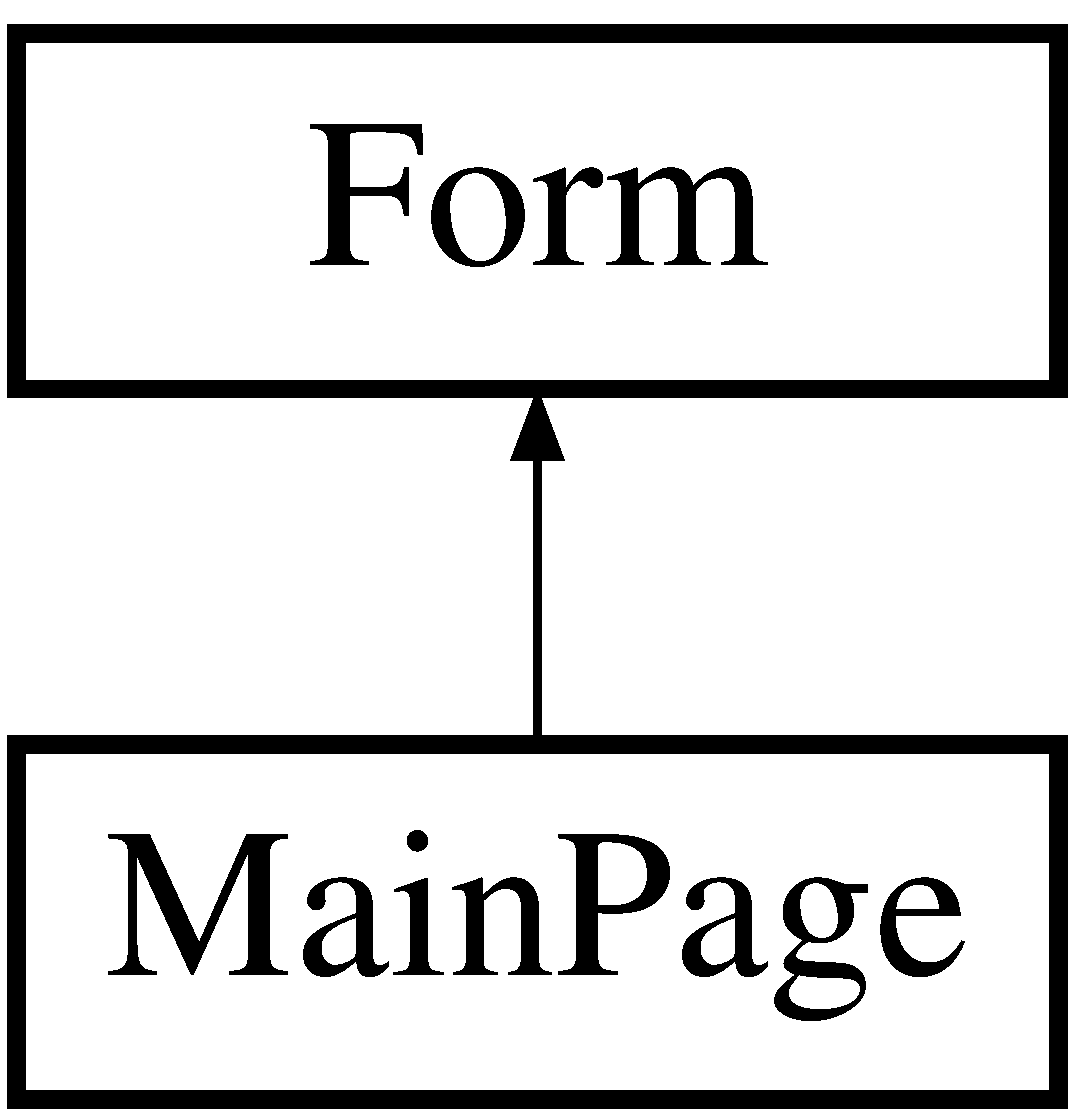
\includegraphics[height=2.000000cm]{classWildlifeTrackingApp_1_1MainPage}
\end{center}
\end{figure}
\subsection*{Public Member Functions}
\begin{DoxyCompactItemize}
\item 
\hyperlink{classWildlifeTrackingApp_1_1MainPage_a6fbc6092ff7046d51931408a67b5e855}{Main\+Page} ()
\end{DoxyCompactItemize}
\subsection*{Protected Member Functions}
\begin{DoxyCompactItemize}
\item 
override void \hyperlink{classWildlifeTrackingApp_1_1MainPage_a849c3c7f8d08104f0cdb46bee9fe6389}{Dispose} (bool disposing)
\begin{DoxyCompactList}\small\item\em Clean up any resources being used. \end{DoxyCompactList}\end{DoxyCompactItemize}
\subsection*{Properties}
\begin{DoxyCompactItemize}
\item 
static log4net.\+I\+Log \hyperlink{classWildlifeTrackingApp_1_1MainPage_a5fc9abb86e6110ecd61d0a1a7d740a8a}{Log}\hspace{0.3cm}{\ttfamily  \mbox{[}get, private set\mbox{]}}
\end{DoxyCompactItemize}
\subsection*{Private Member Functions}
\begin{DoxyCompactItemize}
\item 
void \hyperlink{classWildlifeTrackingApp_1_1MainPage_a66141b70a6e8d761ca0e50ccb9bb5346}{category\+\_\+\+\_\+label\+\_\+\+Click} (object sender, Event\+Args e)
\begin{DoxyCompactList}\small\item\em Event handler for the category selection click. \end{DoxyCompactList}\item 
void \hyperlink{classWildlifeTrackingApp_1_1MainPage_a219fa14b69b49c53c056f1246586ee7c}{Change\+Button\+Color} (Label label)
\begin{DoxyCompactList}\small\item\em Changes the color of label based on selection. \end{DoxyCompactList}\item 
void \hyperlink{classWildlifeTrackingApp_1_1MainPage_ab39f92c5661e132484e3ec3c2be6dbc6}{gps\+Device\+\_\+\+Label\+\_\+\+Click} (object sender, Event\+Args e)
\begin{DoxyCompactList}\small\item\em Event handler for the G\+Ps device selection click. \end{DoxyCompactList}\item 
void \hyperlink{classWildlifeTrackingApp_1_1MainPage_ad3ed7ab0447838e464c2afe0b67e916a}{G\+P\+S\+Device\+\_\+toolstrip\+\_\+\+Item\+Clicked} (object sender, Tool\+Strip\+Item\+Clicked\+Event\+Args e)
\item 
void \hyperlink{classWildlifeTrackingApp_1_1MainPage_a6405d5db675d5338663195a4d12b4c9f}{Initialize\+Component} ()
\begin{DoxyCompactList}\small\item\em Required method for Designer support -\/ do not modify the contents of this method with the code editor. \end{DoxyCompactList}\item 
void \hyperlink{classWildlifeTrackingApp_1_1MainPage_a9f26712bc47d237729adb6b4e9a78356}{locate\+\_\+label\+\_\+\+Click} (object sender, Event\+Args e)
\begin{DoxyCompactList}\small\item\em Event handler for the locate category selection click. \end{DoxyCompactList}\item 
void \hyperlink{classWildlifeTrackingApp_1_1MainPage_ab8756fc3263bdfbe17a118374ab779bc}{main\+Page\+Back\+Ground\+\_\+\+Resize} (object sender, Event\+Args e)
\begin{DoxyCompactList}\small\item\em Event handler for the resizing of the form page. \end{DoxyCompactList}\item 
void \hyperlink{classWildlifeTrackingApp_1_1MainPage_aca7c119833ad4525022a07c4b036e800}{report\+\_\+label\+\_\+\+Click} (object sender, Event\+Args e)
\begin{DoxyCompactList}\small\item\em Event handler for the report selection click. \end{DoxyCompactList}\end{DoxyCompactItemize}
\subsection*{Private Attributes}
\begin{DoxyCompactItemize}
\item 
System.\+Windows.\+Forms.\+Label \hyperlink{classWildlifeTrackingApp_1_1MainPage_ab62919eb07aea9df0b876b7bdf801745}{category\+\_\+\+\_\+label}
\item 
System.\+Windows.\+Forms.\+Tool\+Strip \hyperlink{classWildlifeTrackingApp_1_1MainPage_abf545879da1afeb721121957c32b7ae1}{category\+\_\+tool\+Strip}
\item 
System.\+Component\+Model.\+I\+Container \hyperlink{classWildlifeTrackingApp_1_1MainPage_a02595f1c09713bb71dcb2fbbfc7ffa4b}{components} = null
\begin{DoxyCompactList}\small\item\em Required designer variable. \end{DoxyCompactList}\item 
System.\+Windows.\+Forms.\+Label \hyperlink{classWildlifeTrackingApp_1_1MainPage_ab88680d024b50e48fcf07ba1c7fd1ade}{gps\+Device\+\_\+\+Label}
\item 
System.\+Windows.\+Forms.\+Tool\+Strip \hyperlink{classWildlifeTrackingApp_1_1MainPage_a20432d42ae05e87e11466d593461de02}{G\+P\+S\+Device\+\_\+toolstrip}
\item 
System.\+Windows.\+Forms.\+Label \hyperlink{classWildlifeTrackingApp_1_1MainPage_af84eec8207ceaa0e14076b855415dcea}{locate\+\_\+label}
\item 
System.\+Windows.\+Forms.\+Tool\+Strip \hyperlink{classWildlifeTrackingApp_1_1MainPage_aef30fcc86c717364f65f5a49927f1227}{locate\+\_\+tool\+Strip}
\item 
System.\+Windows.\+Forms.\+Panel \hyperlink{classWildlifeTrackingApp_1_1MainPage_a094665b3f6c785c28d99b6261dc95eb0}{main\+Panel}
\item 
System.\+Windows.\+Forms.\+Label \hyperlink{classWildlifeTrackingApp_1_1MainPage_af6ba70393d92ce2a983bf47ab956b019}{name\+\_\+label}
\item 
System.\+Windows.\+Forms.\+Label \hyperlink{classWildlifeTrackingApp_1_1MainPage_a6c60ee802abc7c2be3dda738a63abc86}{report\+\_\+label}
\item 
System.\+Windows.\+Forms.\+Tool\+Strip \hyperlink{classWildlifeTrackingApp_1_1MainPage_a910f81e378fc8c66e03a986cfa7c5b4d}{report\+\_\+tool\+Strip}
\item 
System.\+Windows.\+Forms.\+Panel \hyperlink{classWildlifeTrackingApp_1_1MainPage_ad9987c4b3ca7748f440a16a357ce86e5}{title\+\_\+\+Panel}
\end{DoxyCompactItemize}
\subsection*{Static Private Attributes}
\begin{DoxyCompactItemize}
\item 
static readonly log4net.\+I\+Log \hyperlink{classWildlifeTrackingApp_1_1MainPage_ae6c6142b8525b2f4ac6ee6e003b3106f}{log}
\end{DoxyCompactItemize}


\subsection{Detailed Description}
Parent Form class which loades the main page of the application. 



\subsection{Constructor \& Destructor Documentation}
\mbox{\Hypertarget{classWildlifeTrackingApp_1_1MainPage_a6fbc6092ff7046d51931408a67b5e855}\label{classWildlifeTrackingApp_1_1MainPage_a6fbc6092ff7046d51931408a67b5e855}} 
\index{Wildlife\+Tracking\+App\+::\+Main\+Page@{Wildlife\+Tracking\+App\+::\+Main\+Page}!Main\+Page@{Main\+Page}}
\index{Main\+Page@{Main\+Page}!Wildlife\+Tracking\+App\+::\+Main\+Page@{Wildlife\+Tracking\+App\+::\+Main\+Page}}
\subsubsection{\texorpdfstring{Main\+Page()}{MainPage()}}
{\footnotesize\ttfamily \hyperlink{classWildlifeTrackingApp_1_1MainPage}{Main\+Page} (\begin{DoxyParamCaption}{ }\end{DoxyParamCaption})\hspace{0.3cm}{\ttfamily [inline]}}



\subsection{Member Function Documentation}
\mbox{\Hypertarget{classWildlifeTrackingApp_1_1MainPage_a66141b70a6e8d761ca0e50ccb9bb5346}\label{classWildlifeTrackingApp_1_1MainPage_a66141b70a6e8d761ca0e50ccb9bb5346}} 
\index{Wildlife\+Tracking\+App\+::\+Main\+Page@{Wildlife\+Tracking\+App\+::\+Main\+Page}!category\+\_\+\+\_\+label\+\_\+\+Click@{category\+\_\+\+\_\+label\+\_\+\+Click}}
\index{category\+\_\+\+\_\+label\+\_\+\+Click@{category\+\_\+\+\_\+label\+\_\+\+Click}!Wildlife\+Tracking\+App\+::\+Main\+Page@{Wildlife\+Tracking\+App\+::\+Main\+Page}}
\subsubsection{\texorpdfstring{category\+\_\+\+\_\+label\+\_\+\+Click()}{category\_\_label\_Click()}}
{\footnotesize\ttfamily void category\+\_\+\+\_\+label\+\_\+\+Click (\begin{DoxyParamCaption}\item[{object}]{sender,  }\item[{Event\+Args}]{e }\end{DoxyParamCaption})\hspace{0.3cm}{\ttfamily [inline]}, {\ttfamily [private]}}



Event handler for the category selection click. 


\begin{DoxyParams}{Parameters}
{\em sender} & Sender Object\\
\hline
{\em e} & Event argument\\
\hline
\end{DoxyParams}
\mbox{\Hypertarget{classWildlifeTrackingApp_1_1MainPage_a219fa14b69b49c53c056f1246586ee7c}\label{classWildlifeTrackingApp_1_1MainPage_a219fa14b69b49c53c056f1246586ee7c}} 
\index{Wildlife\+Tracking\+App\+::\+Main\+Page@{Wildlife\+Tracking\+App\+::\+Main\+Page}!Change\+Button\+Color@{Change\+Button\+Color}}
\index{Change\+Button\+Color@{Change\+Button\+Color}!Wildlife\+Tracking\+App\+::\+Main\+Page@{Wildlife\+Tracking\+App\+::\+Main\+Page}}
\subsubsection{\texorpdfstring{Change\+Button\+Color()}{ChangeButtonColor()}}
{\footnotesize\ttfamily void Change\+Button\+Color (\begin{DoxyParamCaption}\item[{Label}]{label }\end{DoxyParamCaption})\hspace{0.3cm}{\ttfamily [inline]}, {\ttfamily [private]}}



Changes the color of label based on selection. 


\begin{DoxyParams}{Parameters}
{\em label} & Instance of selected label\\
\hline
\end{DoxyParams}
\mbox{\Hypertarget{classWildlifeTrackingApp_1_1MainPage_a849c3c7f8d08104f0cdb46bee9fe6389}\label{classWildlifeTrackingApp_1_1MainPage_a849c3c7f8d08104f0cdb46bee9fe6389}} 
\index{Wildlife\+Tracking\+App\+::\+Main\+Page@{Wildlife\+Tracking\+App\+::\+Main\+Page}!Dispose@{Dispose}}
\index{Dispose@{Dispose}!Wildlife\+Tracking\+App\+::\+Main\+Page@{Wildlife\+Tracking\+App\+::\+Main\+Page}}
\subsubsection{\texorpdfstring{Dispose()}{Dispose()}}
{\footnotesize\ttfamily override void Dispose (\begin{DoxyParamCaption}\item[{bool}]{disposing }\end{DoxyParamCaption})\hspace{0.3cm}{\ttfamily [inline]}, {\ttfamily [protected]}}



Clean up any resources being used. 


\begin{DoxyParams}{Parameters}
{\em disposing} & true if managed resources should be disposed; otherwise, false.\\
\hline
\end{DoxyParams}
\mbox{\Hypertarget{classWildlifeTrackingApp_1_1MainPage_ab39f92c5661e132484e3ec3c2be6dbc6}\label{classWildlifeTrackingApp_1_1MainPage_ab39f92c5661e132484e3ec3c2be6dbc6}} 
\index{Wildlife\+Tracking\+App\+::\+Main\+Page@{Wildlife\+Tracking\+App\+::\+Main\+Page}!gps\+Device\+\_\+\+Label\+\_\+\+Click@{gps\+Device\+\_\+\+Label\+\_\+\+Click}}
\index{gps\+Device\+\_\+\+Label\+\_\+\+Click@{gps\+Device\+\_\+\+Label\+\_\+\+Click}!Wildlife\+Tracking\+App\+::\+Main\+Page@{Wildlife\+Tracking\+App\+::\+Main\+Page}}
\subsubsection{\texorpdfstring{gps\+Device\+\_\+\+Label\+\_\+\+Click()}{gpsDevice\_Label\_Click()}}
{\footnotesize\ttfamily void gps\+Device\+\_\+\+Label\+\_\+\+Click (\begin{DoxyParamCaption}\item[{object}]{sender,  }\item[{Event\+Args}]{e }\end{DoxyParamCaption})\hspace{0.3cm}{\ttfamily [inline]}, {\ttfamily [private]}}



Event handler for the G\+Ps device selection click. 


\begin{DoxyParams}{Parameters}
{\em sender} & Sender Object\\
\hline
{\em e} & Event argument\\
\hline
\end{DoxyParams}
\mbox{\Hypertarget{classWildlifeTrackingApp_1_1MainPage_ad3ed7ab0447838e464c2afe0b67e916a}\label{classWildlifeTrackingApp_1_1MainPage_ad3ed7ab0447838e464c2afe0b67e916a}} 
\index{Wildlife\+Tracking\+App\+::\+Main\+Page@{Wildlife\+Tracking\+App\+::\+Main\+Page}!G\+P\+S\+Device\+\_\+toolstrip\+\_\+\+Item\+Clicked@{G\+P\+S\+Device\+\_\+toolstrip\+\_\+\+Item\+Clicked}}
\index{G\+P\+S\+Device\+\_\+toolstrip\+\_\+\+Item\+Clicked@{G\+P\+S\+Device\+\_\+toolstrip\+\_\+\+Item\+Clicked}!Wildlife\+Tracking\+App\+::\+Main\+Page@{Wildlife\+Tracking\+App\+::\+Main\+Page}}
\subsubsection{\texorpdfstring{G\+P\+S\+Device\+\_\+toolstrip\+\_\+\+Item\+Clicked()}{GPSDevice\_toolstrip\_ItemClicked()}}
{\footnotesize\ttfamily void G\+P\+S\+Device\+\_\+toolstrip\+\_\+\+Item\+Clicked (\begin{DoxyParamCaption}\item[{object}]{sender,  }\item[{Tool\+Strip\+Item\+Clicked\+Event\+Args}]{e }\end{DoxyParamCaption})\hspace{0.3cm}{\ttfamily [inline]}, {\ttfamily [private]}}

\mbox{\Hypertarget{classWildlifeTrackingApp_1_1MainPage_a6405d5db675d5338663195a4d12b4c9f}\label{classWildlifeTrackingApp_1_1MainPage_a6405d5db675d5338663195a4d12b4c9f}} 
\index{Wildlife\+Tracking\+App\+::\+Main\+Page@{Wildlife\+Tracking\+App\+::\+Main\+Page}!Initialize\+Component@{Initialize\+Component}}
\index{Initialize\+Component@{Initialize\+Component}!Wildlife\+Tracking\+App\+::\+Main\+Page@{Wildlife\+Tracking\+App\+::\+Main\+Page}}
\subsubsection{\texorpdfstring{Initialize\+Component()}{InitializeComponent()}}
{\footnotesize\ttfamily void Initialize\+Component (\begin{DoxyParamCaption}{ }\end{DoxyParamCaption})\hspace{0.3cm}{\ttfamily [inline]}, {\ttfamily [private]}}



Required method for Designer support -\/ do not modify the contents of this method with the code editor. 

\mbox{\Hypertarget{classWildlifeTrackingApp_1_1MainPage_a9f26712bc47d237729adb6b4e9a78356}\label{classWildlifeTrackingApp_1_1MainPage_a9f26712bc47d237729adb6b4e9a78356}} 
\index{Wildlife\+Tracking\+App\+::\+Main\+Page@{Wildlife\+Tracking\+App\+::\+Main\+Page}!locate\+\_\+label\+\_\+\+Click@{locate\+\_\+label\+\_\+\+Click}}
\index{locate\+\_\+label\+\_\+\+Click@{locate\+\_\+label\+\_\+\+Click}!Wildlife\+Tracking\+App\+::\+Main\+Page@{Wildlife\+Tracking\+App\+::\+Main\+Page}}
\subsubsection{\texorpdfstring{locate\+\_\+label\+\_\+\+Click()}{locate\_label\_Click()}}
{\footnotesize\ttfamily void locate\+\_\+label\+\_\+\+Click (\begin{DoxyParamCaption}\item[{object}]{sender,  }\item[{Event\+Args}]{e }\end{DoxyParamCaption})\hspace{0.3cm}{\ttfamily [inline]}, {\ttfamily [private]}}



Event handler for the locate category selection click. 


\begin{DoxyParams}{Parameters}
{\em sender} & Sender Object\\
\hline
{\em e} & Event argument\\
\hline
\end{DoxyParams}
\mbox{\Hypertarget{classWildlifeTrackingApp_1_1MainPage_ab8756fc3263bdfbe17a118374ab779bc}\label{classWildlifeTrackingApp_1_1MainPage_ab8756fc3263bdfbe17a118374ab779bc}} 
\index{Wildlife\+Tracking\+App\+::\+Main\+Page@{Wildlife\+Tracking\+App\+::\+Main\+Page}!main\+Page\+Back\+Ground\+\_\+\+Resize@{main\+Page\+Back\+Ground\+\_\+\+Resize}}
\index{main\+Page\+Back\+Ground\+\_\+\+Resize@{main\+Page\+Back\+Ground\+\_\+\+Resize}!Wildlife\+Tracking\+App\+::\+Main\+Page@{Wildlife\+Tracking\+App\+::\+Main\+Page}}
\subsubsection{\texorpdfstring{main\+Page\+Back\+Ground\+\_\+\+Resize()}{mainPageBackGround\_Resize()}}
{\footnotesize\ttfamily void main\+Page\+Back\+Ground\+\_\+\+Resize (\begin{DoxyParamCaption}\item[{object}]{sender,  }\item[{Event\+Args}]{e }\end{DoxyParamCaption})\hspace{0.3cm}{\ttfamily [inline]}, {\ttfamily [private]}}



Event handler for the resizing of the form page. 


\begin{DoxyParams}{Parameters}
{\em sender} & Sender Object\\
\hline
{\em e} & Event argument\\
\hline
\end{DoxyParams}
\mbox{\Hypertarget{classWildlifeTrackingApp_1_1MainPage_aca7c119833ad4525022a07c4b036e800}\label{classWildlifeTrackingApp_1_1MainPage_aca7c119833ad4525022a07c4b036e800}} 
\index{Wildlife\+Tracking\+App\+::\+Main\+Page@{Wildlife\+Tracking\+App\+::\+Main\+Page}!report\+\_\+label\+\_\+\+Click@{report\+\_\+label\+\_\+\+Click}}
\index{report\+\_\+label\+\_\+\+Click@{report\+\_\+label\+\_\+\+Click}!Wildlife\+Tracking\+App\+::\+Main\+Page@{Wildlife\+Tracking\+App\+::\+Main\+Page}}
\subsubsection{\texorpdfstring{report\+\_\+label\+\_\+\+Click()}{report\_label\_Click()}}
{\footnotesize\ttfamily void report\+\_\+label\+\_\+\+Click (\begin{DoxyParamCaption}\item[{object}]{sender,  }\item[{Event\+Args}]{e }\end{DoxyParamCaption})\hspace{0.3cm}{\ttfamily [inline]}, {\ttfamily [private]}}



Event handler for the report selection click. 


\begin{DoxyParams}{Parameters}
{\em sender} & Sender Object\\
\hline
{\em e} & Event argument\\
\hline
\end{DoxyParams}


\subsection{Member Data Documentation}
\mbox{\Hypertarget{classWildlifeTrackingApp_1_1MainPage_ab62919eb07aea9df0b876b7bdf801745}\label{classWildlifeTrackingApp_1_1MainPage_ab62919eb07aea9df0b876b7bdf801745}} 
\index{Wildlife\+Tracking\+App\+::\+Main\+Page@{Wildlife\+Tracking\+App\+::\+Main\+Page}!category\+\_\+\+\_\+label@{category\+\_\+\+\_\+label}}
\index{category\+\_\+\+\_\+label@{category\+\_\+\+\_\+label}!Wildlife\+Tracking\+App\+::\+Main\+Page@{Wildlife\+Tracking\+App\+::\+Main\+Page}}
\subsubsection{\texorpdfstring{category\+\_\+\+\_\+label}{category\_\_label}}
{\footnotesize\ttfamily System.\+Windows.\+Forms.\+Label category\+\_\+\+\_\+label\hspace{0.3cm}{\ttfamily [private]}}

\mbox{\Hypertarget{classWildlifeTrackingApp_1_1MainPage_abf545879da1afeb721121957c32b7ae1}\label{classWildlifeTrackingApp_1_1MainPage_abf545879da1afeb721121957c32b7ae1}} 
\index{Wildlife\+Tracking\+App\+::\+Main\+Page@{Wildlife\+Tracking\+App\+::\+Main\+Page}!category\+\_\+tool\+Strip@{category\+\_\+tool\+Strip}}
\index{category\+\_\+tool\+Strip@{category\+\_\+tool\+Strip}!Wildlife\+Tracking\+App\+::\+Main\+Page@{Wildlife\+Tracking\+App\+::\+Main\+Page}}
\subsubsection{\texorpdfstring{category\+\_\+tool\+Strip}{category\_toolStrip}}
{\footnotesize\ttfamily System.\+Windows.\+Forms.\+Tool\+Strip category\+\_\+tool\+Strip\hspace{0.3cm}{\ttfamily [private]}}

\mbox{\Hypertarget{classWildlifeTrackingApp_1_1MainPage_a02595f1c09713bb71dcb2fbbfc7ffa4b}\label{classWildlifeTrackingApp_1_1MainPage_a02595f1c09713bb71dcb2fbbfc7ffa4b}} 
\index{Wildlife\+Tracking\+App\+::\+Main\+Page@{Wildlife\+Tracking\+App\+::\+Main\+Page}!components@{components}}
\index{components@{components}!Wildlife\+Tracking\+App\+::\+Main\+Page@{Wildlife\+Tracking\+App\+::\+Main\+Page}}
\subsubsection{\texorpdfstring{components}{components}}
{\footnotesize\ttfamily System.\+Component\+Model.\+I\+Container components = null\hspace{0.3cm}{\ttfamily [private]}}



Required designer variable. 

\mbox{\Hypertarget{classWildlifeTrackingApp_1_1MainPage_ab88680d024b50e48fcf07ba1c7fd1ade}\label{classWildlifeTrackingApp_1_1MainPage_ab88680d024b50e48fcf07ba1c7fd1ade}} 
\index{Wildlife\+Tracking\+App\+::\+Main\+Page@{Wildlife\+Tracking\+App\+::\+Main\+Page}!gps\+Device\+\_\+\+Label@{gps\+Device\+\_\+\+Label}}
\index{gps\+Device\+\_\+\+Label@{gps\+Device\+\_\+\+Label}!Wildlife\+Tracking\+App\+::\+Main\+Page@{Wildlife\+Tracking\+App\+::\+Main\+Page}}
\subsubsection{\texorpdfstring{gps\+Device\+\_\+\+Label}{gpsDevice\_Label}}
{\footnotesize\ttfamily System.\+Windows.\+Forms.\+Label gps\+Device\+\_\+\+Label\hspace{0.3cm}{\ttfamily [private]}}

\mbox{\Hypertarget{classWildlifeTrackingApp_1_1MainPage_a20432d42ae05e87e11466d593461de02}\label{classWildlifeTrackingApp_1_1MainPage_a20432d42ae05e87e11466d593461de02}} 
\index{Wildlife\+Tracking\+App\+::\+Main\+Page@{Wildlife\+Tracking\+App\+::\+Main\+Page}!G\+P\+S\+Device\+\_\+toolstrip@{G\+P\+S\+Device\+\_\+toolstrip}}
\index{G\+P\+S\+Device\+\_\+toolstrip@{G\+P\+S\+Device\+\_\+toolstrip}!Wildlife\+Tracking\+App\+::\+Main\+Page@{Wildlife\+Tracking\+App\+::\+Main\+Page}}
\subsubsection{\texorpdfstring{G\+P\+S\+Device\+\_\+toolstrip}{GPSDevice\_toolstrip}}
{\footnotesize\ttfamily System.\+Windows.\+Forms.\+Tool\+Strip G\+P\+S\+Device\+\_\+toolstrip\hspace{0.3cm}{\ttfamily [private]}}

\mbox{\Hypertarget{classWildlifeTrackingApp_1_1MainPage_af84eec8207ceaa0e14076b855415dcea}\label{classWildlifeTrackingApp_1_1MainPage_af84eec8207ceaa0e14076b855415dcea}} 
\index{Wildlife\+Tracking\+App\+::\+Main\+Page@{Wildlife\+Tracking\+App\+::\+Main\+Page}!locate\+\_\+label@{locate\+\_\+label}}
\index{locate\+\_\+label@{locate\+\_\+label}!Wildlife\+Tracking\+App\+::\+Main\+Page@{Wildlife\+Tracking\+App\+::\+Main\+Page}}
\subsubsection{\texorpdfstring{locate\+\_\+label}{locate\_label}}
{\footnotesize\ttfamily System.\+Windows.\+Forms.\+Label locate\+\_\+label\hspace{0.3cm}{\ttfamily [private]}}

\mbox{\Hypertarget{classWildlifeTrackingApp_1_1MainPage_aef30fcc86c717364f65f5a49927f1227}\label{classWildlifeTrackingApp_1_1MainPage_aef30fcc86c717364f65f5a49927f1227}} 
\index{Wildlife\+Tracking\+App\+::\+Main\+Page@{Wildlife\+Tracking\+App\+::\+Main\+Page}!locate\+\_\+tool\+Strip@{locate\+\_\+tool\+Strip}}
\index{locate\+\_\+tool\+Strip@{locate\+\_\+tool\+Strip}!Wildlife\+Tracking\+App\+::\+Main\+Page@{Wildlife\+Tracking\+App\+::\+Main\+Page}}
\subsubsection{\texorpdfstring{locate\+\_\+tool\+Strip}{locate\_toolStrip}}
{\footnotesize\ttfamily System.\+Windows.\+Forms.\+Tool\+Strip locate\+\_\+tool\+Strip\hspace{0.3cm}{\ttfamily [private]}}

\mbox{\Hypertarget{classWildlifeTrackingApp_1_1MainPage_ae6c6142b8525b2f4ac6ee6e003b3106f}\label{classWildlifeTrackingApp_1_1MainPage_ae6c6142b8525b2f4ac6ee6e003b3106f}} 
\index{Wildlife\+Tracking\+App\+::\+Main\+Page@{Wildlife\+Tracking\+App\+::\+Main\+Page}!log@{log}}
\index{log@{log}!Wildlife\+Tracking\+App\+::\+Main\+Page@{Wildlife\+Tracking\+App\+::\+Main\+Page}}
\subsubsection{\texorpdfstring{log}{log}}
{\footnotesize\ttfamily readonly log4net.\+I\+Log log\hspace{0.3cm}{\ttfamily [static]}, {\ttfamily [private]}}

{\bfseries Initial value\+:}
\begin{DoxyCode}
= log4net.LogManager.GetLogger
        (\hyperlink{namespaceSystem}{System}.Reflection.MethodBase.GetCurrentMethod().DeclaringType)
\end{DoxyCode}
\mbox{\Hypertarget{classWildlifeTrackingApp_1_1MainPage_a094665b3f6c785c28d99b6261dc95eb0}\label{classWildlifeTrackingApp_1_1MainPage_a094665b3f6c785c28d99b6261dc95eb0}} 
\index{Wildlife\+Tracking\+App\+::\+Main\+Page@{Wildlife\+Tracking\+App\+::\+Main\+Page}!main\+Panel@{main\+Panel}}
\index{main\+Panel@{main\+Panel}!Wildlife\+Tracking\+App\+::\+Main\+Page@{Wildlife\+Tracking\+App\+::\+Main\+Page}}
\subsubsection{\texorpdfstring{main\+Panel}{mainPanel}}
{\footnotesize\ttfamily System.\+Windows.\+Forms.\+Panel main\+Panel\hspace{0.3cm}{\ttfamily [private]}}

\mbox{\Hypertarget{classWildlifeTrackingApp_1_1MainPage_af6ba70393d92ce2a983bf47ab956b019}\label{classWildlifeTrackingApp_1_1MainPage_af6ba70393d92ce2a983bf47ab956b019}} 
\index{Wildlife\+Tracking\+App\+::\+Main\+Page@{Wildlife\+Tracking\+App\+::\+Main\+Page}!name\+\_\+label@{name\+\_\+label}}
\index{name\+\_\+label@{name\+\_\+label}!Wildlife\+Tracking\+App\+::\+Main\+Page@{Wildlife\+Tracking\+App\+::\+Main\+Page}}
\subsubsection{\texorpdfstring{name\+\_\+label}{name\_label}}
{\footnotesize\ttfamily System.\+Windows.\+Forms.\+Label name\+\_\+label\hspace{0.3cm}{\ttfamily [private]}}

\mbox{\Hypertarget{classWildlifeTrackingApp_1_1MainPage_a6c60ee802abc7c2be3dda738a63abc86}\label{classWildlifeTrackingApp_1_1MainPage_a6c60ee802abc7c2be3dda738a63abc86}} 
\index{Wildlife\+Tracking\+App\+::\+Main\+Page@{Wildlife\+Tracking\+App\+::\+Main\+Page}!report\+\_\+label@{report\+\_\+label}}
\index{report\+\_\+label@{report\+\_\+label}!Wildlife\+Tracking\+App\+::\+Main\+Page@{Wildlife\+Tracking\+App\+::\+Main\+Page}}
\subsubsection{\texorpdfstring{report\+\_\+label}{report\_label}}
{\footnotesize\ttfamily System.\+Windows.\+Forms.\+Label report\+\_\+label\hspace{0.3cm}{\ttfamily [private]}}

\mbox{\Hypertarget{classWildlifeTrackingApp_1_1MainPage_a910f81e378fc8c66e03a986cfa7c5b4d}\label{classWildlifeTrackingApp_1_1MainPage_a910f81e378fc8c66e03a986cfa7c5b4d}} 
\index{Wildlife\+Tracking\+App\+::\+Main\+Page@{Wildlife\+Tracking\+App\+::\+Main\+Page}!report\+\_\+tool\+Strip@{report\+\_\+tool\+Strip}}
\index{report\+\_\+tool\+Strip@{report\+\_\+tool\+Strip}!Wildlife\+Tracking\+App\+::\+Main\+Page@{Wildlife\+Tracking\+App\+::\+Main\+Page}}
\subsubsection{\texorpdfstring{report\+\_\+tool\+Strip}{report\_toolStrip}}
{\footnotesize\ttfamily System.\+Windows.\+Forms.\+Tool\+Strip report\+\_\+tool\+Strip\hspace{0.3cm}{\ttfamily [private]}}

\mbox{\Hypertarget{classWildlifeTrackingApp_1_1MainPage_ad9987c4b3ca7748f440a16a357ce86e5}\label{classWildlifeTrackingApp_1_1MainPage_ad9987c4b3ca7748f440a16a357ce86e5}} 
\index{Wildlife\+Tracking\+App\+::\+Main\+Page@{Wildlife\+Tracking\+App\+::\+Main\+Page}!title\+\_\+\+Panel@{title\+\_\+\+Panel}}
\index{title\+\_\+\+Panel@{title\+\_\+\+Panel}!Wildlife\+Tracking\+App\+::\+Main\+Page@{Wildlife\+Tracking\+App\+::\+Main\+Page}}
\subsubsection{\texorpdfstring{title\+\_\+\+Panel}{title\_Panel}}
{\footnotesize\ttfamily System.\+Windows.\+Forms.\+Panel title\+\_\+\+Panel\hspace{0.3cm}{\ttfamily [private]}}



\subsection{Property Documentation}
\mbox{\Hypertarget{classWildlifeTrackingApp_1_1MainPage_a5fc9abb86e6110ecd61d0a1a7d740a8a}\label{classWildlifeTrackingApp_1_1MainPage_a5fc9abb86e6110ecd61d0a1a7d740a8a}} 
\index{Wildlife\+Tracking\+App\+::\+Main\+Page@{Wildlife\+Tracking\+App\+::\+Main\+Page}!Log@{Log}}
\index{Log@{Log}!Wildlife\+Tracking\+App\+::\+Main\+Page@{Wildlife\+Tracking\+App\+::\+Main\+Page}}
\subsubsection{\texorpdfstring{Log}{Log}}
{\footnotesize\ttfamily log4net.\+I\+Log Log\hspace{0.3cm}{\ttfamily [static]}, {\ttfamily [get]}, {\ttfamily [private set]}}



The documentation for this class was generated from the following files\+:\begin{DoxyCompactItemize}
\item 
View/\hyperlink{MainPage_8cs}{Main\+Page.\+cs}\item 
View/\hyperlink{MainPage_8Designer_8cs}{Main\+Page.\+Designer.\+cs}\end{DoxyCompactItemize}

\hypertarget{classWildlifeTrackingApp_1_1Models_1_1Animal}{}\section{Animal}
\label{classWildlifeTrackingApp_1_1Models_1_1Animal}\index{Animal@{Animal}}


The Model is used for \hyperlink{classWildlifeTrackingApp_1_1Models_1_1Animal}{Animal} Operations.  


\subsection*{Properties}
\begin{DoxyCompactItemize}
\item 
int \hyperlink{classWildlifeTrackingApp_1_1Models_1_1Animal_a99787b9867ae390df467a99040589a55}{animal\+Id}\hspace{0.3cm}{\ttfamily  \mbox{[}get, set\mbox{]}}
\item 
string \hyperlink{classWildlifeTrackingApp_1_1Models_1_1Animal_afd38ba6641283469fc9e94212467f9a2}{animal\+Name}\hspace{0.3cm}{\ttfamily  \mbox{[}get, set\mbox{]}}
\item 
int \hyperlink{classWildlifeTrackingApp_1_1Models_1_1Animal_a423f91c56dc35040d661cfbe357f7c78}{category\+Id}\hspace{0.3cm}{\ttfamily  \mbox{[}get, set\mbox{]}}
\item 
string \hyperlink{classWildlifeTrackingApp_1_1Models_1_1Animal_a1eca787c85e1bc45b49bbd281d4106fd}{category\+Name}\hspace{0.3cm}{\ttfamily  \mbox{[}get, set\mbox{]}}
\item 
string \hyperlink{classWildlifeTrackingApp_1_1Models_1_1Animal_a0ecdefcc99a4b41b1ef3a04167756366}{color\+Indication}\hspace{0.3cm}{\ttfamily  \mbox{[}get, set\mbox{]}}
\item 
string \hyperlink{classWildlifeTrackingApp_1_1Models_1_1Animal_a073b88a9702ca0513fa534f58a048070}{gps\+Device\+Id}\hspace{0.3cm}{\ttfamily  \mbox{[}get, set\mbox{]}}
\item 
int \hyperlink{classWildlifeTrackingApp_1_1Models_1_1Animal_af2a3c76f434001a3f47c287cc16f04ff}{total\+Animals}\hspace{0.3cm}{\ttfamily  \mbox{[}get, set\mbox{]}}
\end{DoxyCompactItemize}


\subsection{Detailed Description}
The Model is used for \hyperlink{classWildlifeTrackingApp_1_1Models_1_1Animal}{Animal} Operations. 



\subsection{Property Documentation}
\mbox{\Hypertarget{classWildlifeTrackingApp_1_1Models_1_1Animal_a99787b9867ae390df467a99040589a55}\label{classWildlifeTrackingApp_1_1Models_1_1Animal_a99787b9867ae390df467a99040589a55}} 
\index{Wildlife\+Tracking\+App\+::\+Models\+::\+Animal@{Wildlife\+Tracking\+App\+::\+Models\+::\+Animal}!animal\+Id@{animal\+Id}}
\index{animal\+Id@{animal\+Id}!Wildlife\+Tracking\+App\+::\+Models\+::\+Animal@{Wildlife\+Tracking\+App\+::\+Models\+::\+Animal}}
\subsubsection{\texorpdfstring{animal\+Id}{animalId}}
{\footnotesize\ttfamily int animal\+Id\hspace{0.3cm}{\ttfamily [get]}, {\ttfamily [set]}}

\mbox{\Hypertarget{classWildlifeTrackingApp_1_1Models_1_1Animal_afd38ba6641283469fc9e94212467f9a2}\label{classWildlifeTrackingApp_1_1Models_1_1Animal_afd38ba6641283469fc9e94212467f9a2}} 
\index{Wildlife\+Tracking\+App\+::\+Models\+::\+Animal@{Wildlife\+Tracking\+App\+::\+Models\+::\+Animal}!animal\+Name@{animal\+Name}}
\index{animal\+Name@{animal\+Name}!Wildlife\+Tracking\+App\+::\+Models\+::\+Animal@{Wildlife\+Tracking\+App\+::\+Models\+::\+Animal}}
\subsubsection{\texorpdfstring{animal\+Name}{animalName}}
{\footnotesize\ttfamily string animal\+Name\hspace{0.3cm}{\ttfamily [get]}, {\ttfamily [set]}}

\mbox{\Hypertarget{classWildlifeTrackingApp_1_1Models_1_1Animal_a423f91c56dc35040d661cfbe357f7c78}\label{classWildlifeTrackingApp_1_1Models_1_1Animal_a423f91c56dc35040d661cfbe357f7c78}} 
\index{Wildlife\+Tracking\+App\+::\+Models\+::\+Animal@{Wildlife\+Tracking\+App\+::\+Models\+::\+Animal}!category\+Id@{category\+Id}}
\index{category\+Id@{category\+Id}!Wildlife\+Tracking\+App\+::\+Models\+::\+Animal@{Wildlife\+Tracking\+App\+::\+Models\+::\+Animal}}
\subsubsection{\texorpdfstring{category\+Id}{categoryId}}
{\footnotesize\ttfamily int category\+Id\hspace{0.3cm}{\ttfamily [get]}, {\ttfamily [set]}}

\mbox{\Hypertarget{classWildlifeTrackingApp_1_1Models_1_1Animal_a1eca787c85e1bc45b49bbd281d4106fd}\label{classWildlifeTrackingApp_1_1Models_1_1Animal_a1eca787c85e1bc45b49bbd281d4106fd}} 
\index{Wildlife\+Tracking\+App\+::\+Models\+::\+Animal@{Wildlife\+Tracking\+App\+::\+Models\+::\+Animal}!category\+Name@{category\+Name}}
\index{category\+Name@{category\+Name}!Wildlife\+Tracking\+App\+::\+Models\+::\+Animal@{Wildlife\+Tracking\+App\+::\+Models\+::\+Animal}}
\subsubsection{\texorpdfstring{category\+Name}{categoryName}}
{\footnotesize\ttfamily string category\+Name\hspace{0.3cm}{\ttfamily [get]}, {\ttfamily [set]}}

\mbox{\Hypertarget{classWildlifeTrackingApp_1_1Models_1_1Animal_a0ecdefcc99a4b41b1ef3a04167756366}\label{classWildlifeTrackingApp_1_1Models_1_1Animal_a0ecdefcc99a4b41b1ef3a04167756366}} 
\index{Wildlife\+Tracking\+App\+::\+Models\+::\+Animal@{Wildlife\+Tracking\+App\+::\+Models\+::\+Animal}!color\+Indication@{color\+Indication}}
\index{color\+Indication@{color\+Indication}!Wildlife\+Tracking\+App\+::\+Models\+::\+Animal@{Wildlife\+Tracking\+App\+::\+Models\+::\+Animal}}
\subsubsection{\texorpdfstring{color\+Indication}{colorIndication}}
{\footnotesize\ttfamily string color\+Indication\hspace{0.3cm}{\ttfamily [get]}, {\ttfamily [set]}}

\mbox{\Hypertarget{classWildlifeTrackingApp_1_1Models_1_1Animal_a073b88a9702ca0513fa534f58a048070}\label{classWildlifeTrackingApp_1_1Models_1_1Animal_a073b88a9702ca0513fa534f58a048070}} 
\index{Wildlife\+Tracking\+App\+::\+Models\+::\+Animal@{Wildlife\+Tracking\+App\+::\+Models\+::\+Animal}!gps\+Device\+Id@{gps\+Device\+Id}}
\index{gps\+Device\+Id@{gps\+Device\+Id}!Wildlife\+Tracking\+App\+::\+Models\+::\+Animal@{Wildlife\+Tracking\+App\+::\+Models\+::\+Animal}}
\subsubsection{\texorpdfstring{gps\+Device\+Id}{gpsDeviceId}}
{\footnotesize\ttfamily string gps\+Device\+Id\hspace{0.3cm}{\ttfamily [get]}, {\ttfamily [set]}}

\mbox{\Hypertarget{classWildlifeTrackingApp_1_1Models_1_1Animal_af2a3c76f434001a3f47c287cc16f04ff}\label{classWildlifeTrackingApp_1_1Models_1_1Animal_af2a3c76f434001a3f47c287cc16f04ff}} 
\index{Wildlife\+Tracking\+App\+::\+Models\+::\+Animal@{Wildlife\+Tracking\+App\+::\+Models\+::\+Animal}!total\+Animals@{total\+Animals}}
\index{total\+Animals@{total\+Animals}!Wildlife\+Tracking\+App\+::\+Models\+::\+Animal@{Wildlife\+Tracking\+App\+::\+Models\+::\+Animal}}
\subsubsection{\texorpdfstring{total\+Animals}{totalAnimals}}
{\footnotesize\ttfamily int total\+Animals\hspace{0.3cm}{\ttfamily [get]}, {\ttfamily [set]}}



The documentation for this class was generated from the following file\+:\begin{DoxyCompactItemize}
\item 
Models/\hyperlink{Animal_8cs}{Animal.\+cs}\end{DoxyCompactItemize}

\hypertarget{classWildlifeTrackingApp_1_1Models_1_1AnimalCategoryCount}{}\section{Animal\+Category\+Count}
\label{classWildlifeTrackingApp_1_1Models_1_1AnimalCategoryCount}\index{Animal\+Category\+Count@{Animal\+Category\+Count}}


The Model is used for Animals Count Per \hyperlink{classWildlifeTrackingApp_1_1Models_1_1Category}{Category}.  


\subsection*{Properties}
\begin{DoxyCompactItemize}
\item 
int \hyperlink{classWildlifeTrackingApp_1_1Models_1_1AnimalCategoryCount_a423f91c56dc35040d661cfbe357f7c78}{category\+Id}\hspace{0.3cm}{\ttfamily  \mbox{[}get, set\mbox{]}}
\item 
string \hyperlink{classWildlifeTrackingApp_1_1Models_1_1AnimalCategoryCount_a1eca787c85e1bc45b49bbd281d4106fd}{category\+Name}\hspace{0.3cm}{\ttfamily  \mbox{[}get, set\mbox{]}}
\item 
string \hyperlink{classWildlifeTrackingApp_1_1Models_1_1AnimalCategoryCount_a0ecdefcc99a4b41b1ef3a04167756366}{color\+Indication}\hspace{0.3cm}{\ttfamily  \mbox{[}get, set\mbox{]}}
\item 
int \hyperlink{classWildlifeTrackingApp_1_1Models_1_1AnimalCategoryCount_af2a3c76f434001a3f47c287cc16f04ff}{total\+Animals}\hspace{0.3cm}{\ttfamily  \mbox{[}get, set\mbox{]}}
\end{DoxyCompactItemize}


\subsection{Detailed Description}
The Model is used for Animals Count Per \hyperlink{classWildlifeTrackingApp_1_1Models_1_1Category}{Category}. 



\subsection{Property Documentation}
\mbox{\Hypertarget{classWildlifeTrackingApp_1_1Models_1_1AnimalCategoryCount_a423f91c56dc35040d661cfbe357f7c78}\label{classWildlifeTrackingApp_1_1Models_1_1AnimalCategoryCount_a423f91c56dc35040d661cfbe357f7c78}} 
\index{Wildlife\+Tracking\+App\+::\+Models\+::\+Animal\+Category\+Count@{Wildlife\+Tracking\+App\+::\+Models\+::\+Animal\+Category\+Count}!category\+Id@{category\+Id}}
\index{category\+Id@{category\+Id}!Wildlife\+Tracking\+App\+::\+Models\+::\+Animal\+Category\+Count@{Wildlife\+Tracking\+App\+::\+Models\+::\+Animal\+Category\+Count}}
\subsubsection{\texorpdfstring{category\+Id}{categoryId}}
{\footnotesize\ttfamily int category\+Id\hspace{0.3cm}{\ttfamily [get]}, {\ttfamily [set]}}

\mbox{\Hypertarget{classWildlifeTrackingApp_1_1Models_1_1AnimalCategoryCount_a1eca787c85e1bc45b49bbd281d4106fd}\label{classWildlifeTrackingApp_1_1Models_1_1AnimalCategoryCount_a1eca787c85e1bc45b49bbd281d4106fd}} 
\index{Wildlife\+Tracking\+App\+::\+Models\+::\+Animal\+Category\+Count@{Wildlife\+Tracking\+App\+::\+Models\+::\+Animal\+Category\+Count}!category\+Name@{category\+Name}}
\index{category\+Name@{category\+Name}!Wildlife\+Tracking\+App\+::\+Models\+::\+Animal\+Category\+Count@{Wildlife\+Tracking\+App\+::\+Models\+::\+Animal\+Category\+Count}}
\subsubsection{\texorpdfstring{category\+Name}{categoryName}}
{\footnotesize\ttfamily string category\+Name\hspace{0.3cm}{\ttfamily [get]}, {\ttfamily [set]}}

\mbox{\Hypertarget{classWildlifeTrackingApp_1_1Models_1_1AnimalCategoryCount_a0ecdefcc99a4b41b1ef3a04167756366}\label{classWildlifeTrackingApp_1_1Models_1_1AnimalCategoryCount_a0ecdefcc99a4b41b1ef3a04167756366}} 
\index{Wildlife\+Tracking\+App\+::\+Models\+::\+Animal\+Category\+Count@{Wildlife\+Tracking\+App\+::\+Models\+::\+Animal\+Category\+Count}!color\+Indication@{color\+Indication}}
\index{color\+Indication@{color\+Indication}!Wildlife\+Tracking\+App\+::\+Models\+::\+Animal\+Category\+Count@{Wildlife\+Tracking\+App\+::\+Models\+::\+Animal\+Category\+Count}}
\subsubsection{\texorpdfstring{color\+Indication}{colorIndication}}
{\footnotesize\ttfamily string color\+Indication\hspace{0.3cm}{\ttfamily [get]}, {\ttfamily [set]}}

\mbox{\Hypertarget{classWildlifeTrackingApp_1_1Models_1_1AnimalCategoryCount_af2a3c76f434001a3f47c287cc16f04ff}\label{classWildlifeTrackingApp_1_1Models_1_1AnimalCategoryCount_af2a3c76f434001a3f47c287cc16f04ff}} 
\index{Wildlife\+Tracking\+App\+::\+Models\+::\+Animal\+Category\+Count@{Wildlife\+Tracking\+App\+::\+Models\+::\+Animal\+Category\+Count}!total\+Animals@{total\+Animals}}
\index{total\+Animals@{total\+Animals}!Wildlife\+Tracking\+App\+::\+Models\+::\+Animal\+Category\+Count@{Wildlife\+Tracking\+App\+::\+Models\+::\+Animal\+Category\+Count}}
\subsubsection{\texorpdfstring{total\+Animals}{totalAnimals}}
{\footnotesize\ttfamily int total\+Animals\hspace{0.3cm}{\ttfamily [get]}, {\ttfamily [set]}}



The documentation for this class was generated from the following file\+:\begin{DoxyCompactItemize}
\item 
Models/\hyperlink{AnimalCategoryCount_8cs}{Animal\+Category\+Count.\+cs}\end{DoxyCompactItemize}

\hypertarget{classWildlifeTrackingApp_1_1Models_1_1AnimalResponseView}{}\section{Animal\+Response\+View}
\label{classWildlifeTrackingApp_1_1Models_1_1AnimalResponseView}\index{Animal\+Response\+View@{Animal\+Response\+View}}


The Model is used for \hyperlink{classWildlifeTrackingApp_1_1Models_1_1Animal}{Animal} \hyperlink{classWildlifeTrackingApp_1_1Models_1_1Response}{Response} from the services.  


\subsection*{Properties}
\begin{DoxyCompactItemize}
\item 
\hyperlink{classWildlifeTrackingApp_1_1Models_1_1Animal}{Animal} \hyperlink{classWildlifeTrackingApp_1_1Models_1_1AnimalResponseView_a364c7e4092980c5a9be7c56a2c810c18}{animal}\hspace{0.3cm}{\ttfamily  \mbox{[}get, set\mbox{]}}
\item 
List$<$ \hyperlink{classWildlifeTrackingApp_1_1Models_1_1Animal}{Animal} $>$ \hyperlink{classWildlifeTrackingApp_1_1Models_1_1AnimalResponseView_a4c541d3fabb48f76436375ec172d1f8f}{animal\+List}\hspace{0.3cm}{\ttfamily  \mbox{[}get, set\mbox{]}}
\item 
List$<$ \hyperlink{classWildlifeTrackingApp_1_1Models_1_1AnimalCategoryCount}{Animal\+Category\+Count} $>$ \hyperlink{classWildlifeTrackingApp_1_1Models_1_1AnimalResponseView_ac145fa4f68cbab144df205048ae7b752}{total\+Animal\+Details}\hspace{0.3cm}{\ttfamily  \mbox{[}get, set\mbox{]}}
\end{DoxyCompactItemize}


\subsection{Detailed Description}
The Model is used for \hyperlink{classWildlifeTrackingApp_1_1Models_1_1Animal}{Animal} \hyperlink{classWildlifeTrackingApp_1_1Models_1_1Response}{Response} from the services. 



\subsection{Property Documentation}
\mbox{\Hypertarget{classWildlifeTrackingApp_1_1Models_1_1AnimalResponseView_a364c7e4092980c5a9be7c56a2c810c18}\label{classWildlifeTrackingApp_1_1Models_1_1AnimalResponseView_a364c7e4092980c5a9be7c56a2c810c18}} 
\index{Wildlife\+Tracking\+App\+::\+Models\+::\+Animal\+Response\+View@{Wildlife\+Tracking\+App\+::\+Models\+::\+Animal\+Response\+View}!animal@{animal}}
\index{animal@{animal}!Wildlife\+Tracking\+App\+::\+Models\+::\+Animal\+Response\+View@{Wildlife\+Tracking\+App\+::\+Models\+::\+Animal\+Response\+View}}
\subsubsection{\texorpdfstring{animal}{animal}}
{\footnotesize\ttfamily \hyperlink{classWildlifeTrackingApp_1_1Models_1_1Animal}{Animal} animal\hspace{0.3cm}{\ttfamily [get]}, {\ttfamily [set]}}

\mbox{\Hypertarget{classWildlifeTrackingApp_1_1Models_1_1AnimalResponseView_a4c541d3fabb48f76436375ec172d1f8f}\label{classWildlifeTrackingApp_1_1Models_1_1AnimalResponseView_a4c541d3fabb48f76436375ec172d1f8f}} 
\index{Wildlife\+Tracking\+App\+::\+Models\+::\+Animal\+Response\+View@{Wildlife\+Tracking\+App\+::\+Models\+::\+Animal\+Response\+View}!animal\+List@{animal\+List}}
\index{animal\+List@{animal\+List}!Wildlife\+Tracking\+App\+::\+Models\+::\+Animal\+Response\+View@{Wildlife\+Tracking\+App\+::\+Models\+::\+Animal\+Response\+View}}
\subsubsection{\texorpdfstring{animal\+List}{animalList}}
{\footnotesize\ttfamily List$<$\hyperlink{classWildlifeTrackingApp_1_1Models_1_1Animal}{Animal}$>$ animal\+List\hspace{0.3cm}{\ttfamily [get]}, {\ttfamily [set]}}

\mbox{\Hypertarget{classWildlifeTrackingApp_1_1Models_1_1AnimalResponseView_ac145fa4f68cbab144df205048ae7b752}\label{classWildlifeTrackingApp_1_1Models_1_1AnimalResponseView_ac145fa4f68cbab144df205048ae7b752}} 
\index{Wildlife\+Tracking\+App\+::\+Models\+::\+Animal\+Response\+View@{Wildlife\+Tracking\+App\+::\+Models\+::\+Animal\+Response\+View}!total\+Animal\+Details@{total\+Animal\+Details}}
\index{total\+Animal\+Details@{total\+Animal\+Details}!Wildlife\+Tracking\+App\+::\+Models\+::\+Animal\+Response\+View@{Wildlife\+Tracking\+App\+::\+Models\+::\+Animal\+Response\+View}}
\subsubsection{\texorpdfstring{total\+Animal\+Details}{totalAnimalDetails}}
{\footnotesize\ttfamily List$<$\hyperlink{classWildlifeTrackingApp_1_1Models_1_1AnimalCategoryCount}{Animal\+Category\+Count}$>$ total\+Animal\+Details\hspace{0.3cm}{\ttfamily [get]}, {\ttfamily [set]}}



The documentation for this class was generated from the following file\+:\begin{DoxyCompactItemize}
\item 
Models/\hyperlink{AnimalResponseView_8cs}{Animal\+Response\+View.\+cs}\end{DoxyCompactItemize}

\hypertarget{classWildlifeTrackingApp_1_1Models_1_1Category}{}\section{Category}
\label{classWildlifeTrackingApp_1_1Models_1_1Category}\index{Category@{Category}}


The Model is used for \hyperlink{classWildlifeTrackingApp_1_1Models_1_1Category}{Category} Operations.  


Inheritance diagram for Category\+:\begin{figure}[H]
\begin{center}
\leavevmode
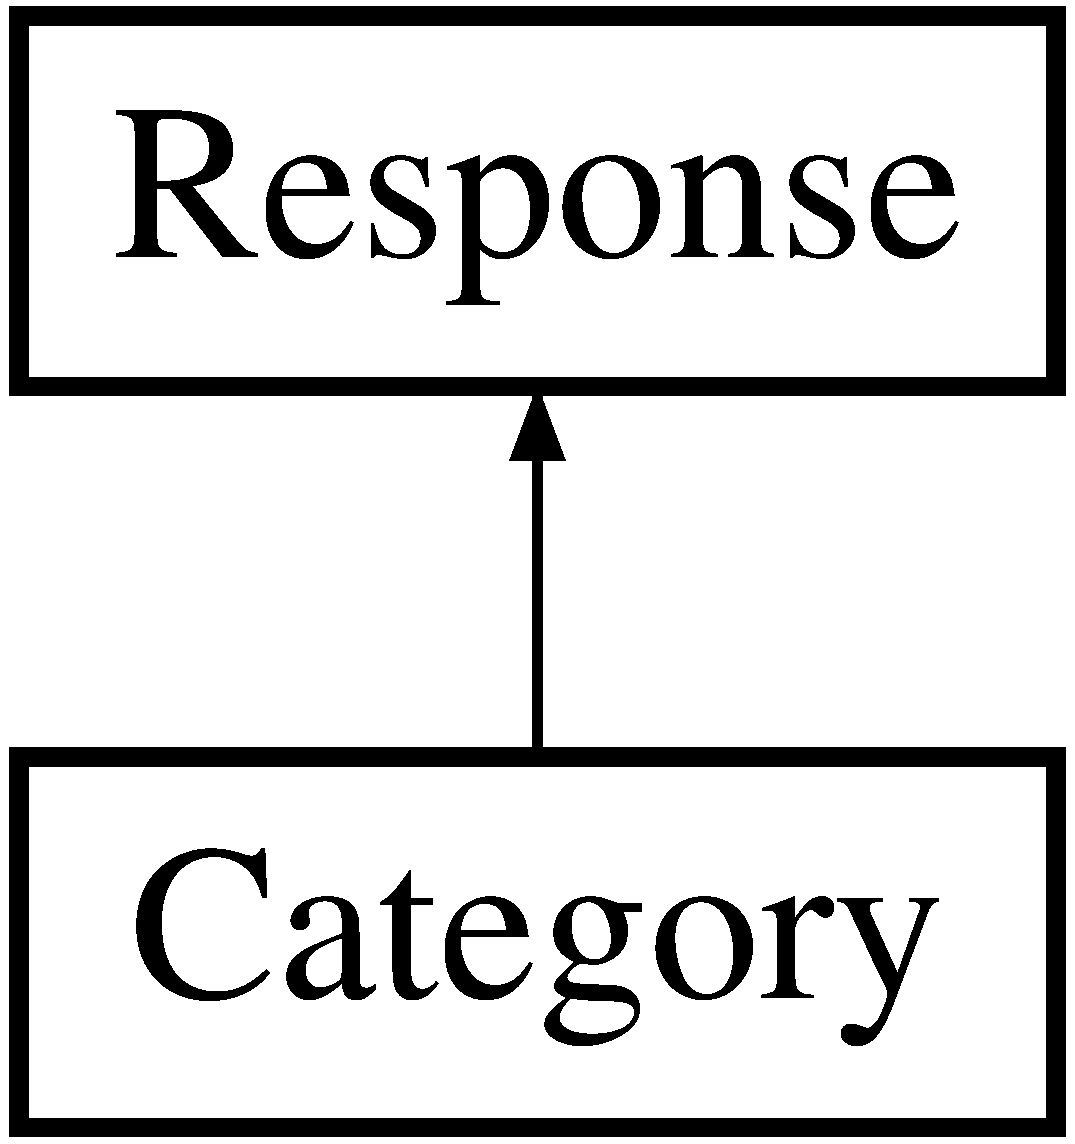
\includegraphics[height=2.000000cm]{classWildlifeTrackingApp_1_1Models_1_1Category}
\end{center}
\end{figure}
\subsection*{Properties}
\begin{DoxyCompactItemize}
\item 
string \hyperlink{classWildlifeTrackingApp_1_1Models_1_1Category_ae992743f1fc0d9386b609d8871a4bd6b}{category\+Desc}\hspace{0.3cm}{\ttfamily  \mbox{[}get, set\mbox{]}}
\item 
int \hyperlink{classWildlifeTrackingApp_1_1Models_1_1Category_a423f91c56dc35040d661cfbe357f7c78}{category\+Id}\hspace{0.3cm}{\ttfamily  \mbox{[}get, set\mbox{]}}
\item 
string \hyperlink{classWildlifeTrackingApp_1_1Models_1_1Category_a1eca787c85e1bc45b49bbd281d4106fd}{category\+Name}\hspace{0.3cm}{\ttfamily  \mbox{[}get, set\mbox{]}}
\item 
string \hyperlink{classWildlifeTrackingApp_1_1Models_1_1Category_a0ecdefcc99a4b41b1ef3a04167756366}{color\+Indication}\hspace{0.3cm}{\ttfamily  \mbox{[}get, set\mbox{]}}
\end{DoxyCompactItemize}


\subsection{Detailed Description}
The Model is used for \hyperlink{classWildlifeTrackingApp_1_1Models_1_1Category}{Category} Operations. 



\subsection{Property Documentation}
\mbox{\Hypertarget{classWildlifeTrackingApp_1_1Models_1_1Category_ae992743f1fc0d9386b609d8871a4bd6b}\label{classWildlifeTrackingApp_1_1Models_1_1Category_ae992743f1fc0d9386b609d8871a4bd6b}} 
\index{Wildlife\+Tracking\+App\+::\+Models\+::\+Category@{Wildlife\+Tracking\+App\+::\+Models\+::\+Category}!category\+Desc@{category\+Desc}}
\index{category\+Desc@{category\+Desc}!Wildlife\+Tracking\+App\+::\+Models\+::\+Category@{Wildlife\+Tracking\+App\+::\+Models\+::\+Category}}
\subsubsection{\texorpdfstring{category\+Desc}{categoryDesc}}
{\footnotesize\ttfamily string category\+Desc\hspace{0.3cm}{\ttfamily [get]}, {\ttfamily [set]}}

\mbox{\Hypertarget{classWildlifeTrackingApp_1_1Models_1_1Category_a423f91c56dc35040d661cfbe357f7c78}\label{classWildlifeTrackingApp_1_1Models_1_1Category_a423f91c56dc35040d661cfbe357f7c78}} 
\index{Wildlife\+Tracking\+App\+::\+Models\+::\+Category@{Wildlife\+Tracking\+App\+::\+Models\+::\+Category}!category\+Id@{category\+Id}}
\index{category\+Id@{category\+Id}!Wildlife\+Tracking\+App\+::\+Models\+::\+Category@{Wildlife\+Tracking\+App\+::\+Models\+::\+Category}}
\subsubsection{\texorpdfstring{category\+Id}{categoryId}}
{\footnotesize\ttfamily int category\+Id\hspace{0.3cm}{\ttfamily [get]}, {\ttfamily [set]}}

\mbox{\Hypertarget{classWildlifeTrackingApp_1_1Models_1_1Category_a1eca787c85e1bc45b49bbd281d4106fd}\label{classWildlifeTrackingApp_1_1Models_1_1Category_a1eca787c85e1bc45b49bbd281d4106fd}} 
\index{Wildlife\+Tracking\+App\+::\+Models\+::\+Category@{Wildlife\+Tracking\+App\+::\+Models\+::\+Category}!category\+Name@{category\+Name}}
\index{category\+Name@{category\+Name}!Wildlife\+Tracking\+App\+::\+Models\+::\+Category@{Wildlife\+Tracking\+App\+::\+Models\+::\+Category}}
\subsubsection{\texorpdfstring{category\+Name}{categoryName}}
{\footnotesize\ttfamily string category\+Name\hspace{0.3cm}{\ttfamily [get]}, {\ttfamily [set]}}

\mbox{\Hypertarget{classWildlifeTrackingApp_1_1Models_1_1Category_a0ecdefcc99a4b41b1ef3a04167756366}\label{classWildlifeTrackingApp_1_1Models_1_1Category_a0ecdefcc99a4b41b1ef3a04167756366}} 
\index{Wildlife\+Tracking\+App\+::\+Models\+::\+Category@{Wildlife\+Tracking\+App\+::\+Models\+::\+Category}!color\+Indication@{color\+Indication}}
\index{color\+Indication@{color\+Indication}!Wildlife\+Tracking\+App\+::\+Models\+::\+Category@{Wildlife\+Tracking\+App\+::\+Models\+::\+Category}}
\subsubsection{\texorpdfstring{color\+Indication}{colorIndication}}
{\footnotesize\ttfamily string color\+Indication\hspace{0.3cm}{\ttfamily [get]}, {\ttfamily [set]}}



The documentation for this class was generated from the following file\+:\begin{DoxyCompactItemize}
\item 
Models/\hyperlink{Models_2Category_8cs}{Category.\+cs}\end{DoxyCompactItemize}

\hypertarget{classWildlifeTrackingApp_1_1Models_1_1CategoryResponseView}{}\section{Category\+Response\+View}
\label{classWildlifeTrackingApp_1_1Models_1_1CategoryResponseView}\index{Category\+Response\+View@{Category\+Response\+View}}


The Model is used for \hyperlink{classWildlifeTrackingApp_1_1Models_1_1Category}{Category} \hyperlink{classWildlifeTrackingApp_1_1Models_1_1Response}{Response} from the service.  


\subsection*{Properties}
\begin{DoxyCompactItemize}
\item 
\hyperlink{classWildlifeTrackingApp_1_1Models_1_1Category}{Category} \hyperlink{classWildlifeTrackingApp_1_1Models_1_1CategoryResponseView_a08b424ccd4f519f4a97826f9d3f3f094}{category}\hspace{0.3cm}{\ttfamily  \mbox{[}get, set\mbox{]}}
\item 
List$<$ \hyperlink{classWildlifeTrackingApp_1_1Models_1_1Category}{Category} $>$ \hyperlink{classWildlifeTrackingApp_1_1Models_1_1CategoryResponseView_ac20f04846190de6a34eadd21501afae3}{category\+List}\hspace{0.3cm}{\ttfamily  \mbox{[}get, set\mbox{]}}
\end{DoxyCompactItemize}


\subsection{Detailed Description}
The Model is used for \hyperlink{classWildlifeTrackingApp_1_1Models_1_1Category}{Category} \hyperlink{classWildlifeTrackingApp_1_1Models_1_1Response}{Response} from the service. 



\subsection{Property Documentation}
\mbox{\Hypertarget{classWildlifeTrackingApp_1_1Models_1_1CategoryResponseView_a08b424ccd4f519f4a97826f9d3f3f094}\label{classWildlifeTrackingApp_1_1Models_1_1CategoryResponseView_a08b424ccd4f519f4a97826f9d3f3f094}} 
\index{Wildlife\+Tracking\+App\+::\+Models\+::\+Category\+Response\+View@{Wildlife\+Tracking\+App\+::\+Models\+::\+Category\+Response\+View}!category@{category}}
\index{category@{category}!Wildlife\+Tracking\+App\+::\+Models\+::\+Category\+Response\+View@{Wildlife\+Tracking\+App\+::\+Models\+::\+Category\+Response\+View}}
\subsubsection{\texorpdfstring{category}{category}}
{\footnotesize\ttfamily \hyperlink{classWildlifeTrackingApp_1_1Models_1_1Category}{Category} category\hspace{0.3cm}{\ttfamily [get]}, {\ttfamily [set]}}

\mbox{\Hypertarget{classWildlifeTrackingApp_1_1Models_1_1CategoryResponseView_ac20f04846190de6a34eadd21501afae3}\label{classWildlifeTrackingApp_1_1Models_1_1CategoryResponseView_ac20f04846190de6a34eadd21501afae3}} 
\index{Wildlife\+Tracking\+App\+::\+Models\+::\+Category\+Response\+View@{Wildlife\+Tracking\+App\+::\+Models\+::\+Category\+Response\+View}!category\+List@{category\+List}}
\index{category\+List@{category\+List}!Wildlife\+Tracking\+App\+::\+Models\+::\+Category\+Response\+View@{Wildlife\+Tracking\+App\+::\+Models\+::\+Category\+Response\+View}}
\subsubsection{\texorpdfstring{category\+List}{categoryList}}
{\footnotesize\ttfamily List$<$\hyperlink{classWildlifeTrackingApp_1_1Models_1_1Category}{Category}$>$ category\+List\hspace{0.3cm}{\ttfamily [get]}, {\ttfamily [set]}}



The documentation for this class was generated from the following file\+:\begin{DoxyCompactItemize}
\item 
Models/\hyperlink{CategoryResponseView_8cs}{Category\+Response\+View.\+cs}\end{DoxyCompactItemize}

\hypertarget{classWildlifeTrackingApp_1_1Models_1_1Response}{}\section{Response}
\label{classWildlifeTrackingApp_1_1Models_1_1Response}\index{Response@{Response}}


The Model is used for recieving message from service.  


Inheritance diagram for Response\+:\begin{figure}[H]
\begin{center}
\leavevmode
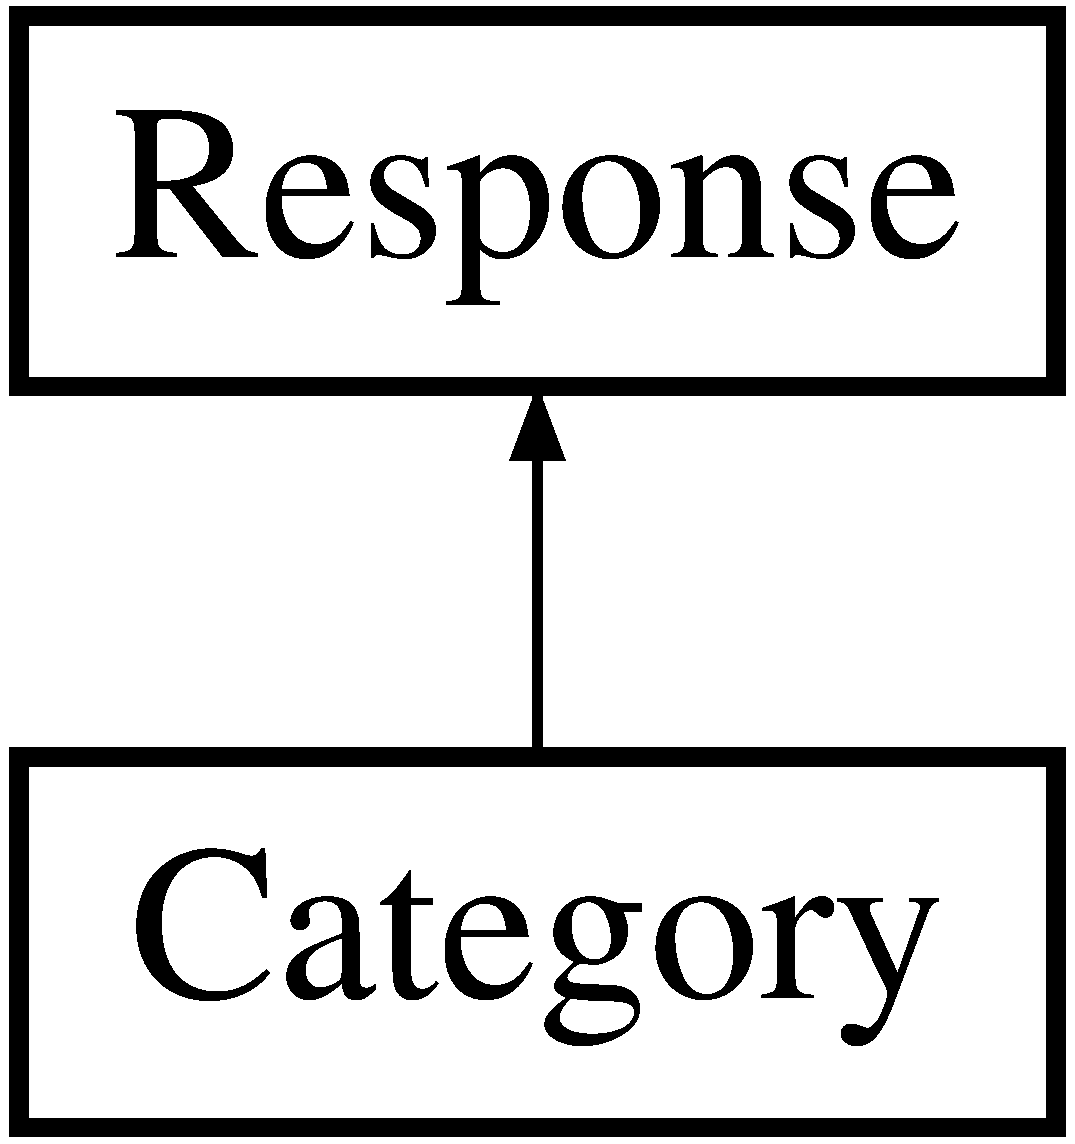
\includegraphics[height=2.000000cm]{classWildlifeTrackingApp_1_1Models_1_1Response}
\end{center}
\end{figure}
\subsection*{Properties}
\begin{DoxyCompactItemize}
\item 
string \hyperlink{classWildlifeTrackingApp_1_1Models_1_1Response_ae1ed0d7a6f352c7ee3ad978429822c6f}{message}\hspace{0.3cm}{\ttfamily  \mbox{[}get, set\mbox{]}}
\end{DoxyCompactItemize}


\subsection{Detailed Description}
The Model is used for recieving message from service. 



\subsection{Property Documentation}
\mbox{\Hypertarget{classWildlifeTrackingApp_1_1Models_1_1Response_ae1ed0d7a6f352c7ee3ad978429822c6f}\label{classWildlifeTrackingApp_1_1Models_1_1Response_ae1ed0d7a6f352c7ee3ad978429822c6f}} 
\index{Wildlife\+Tracking\+App\+::\+Models\+::\+Response@{Wildlife\+Tracking\+App\+::\+Models\+::\+Response}!message@{message}}
\index{message@{message}!Wildlife\+Tracking\+App\+::\+Models\+::\+Response@{Wildlife\+Tracking\+App\+::\+Models\+::\+Response}}
\subsubsection{\texorpdfstring{message}{message}}
{\footnotesize\ttfamily string message\hspace{0.3cm}{\ttfamily [get]}, {\ttfamily [set]}}



The documentation for this class was generated from the following file\+:\begin{DoxyCompactItemize}
\item 
Models/\hyperlink{Response_8cs}{Response.\+cs}\end{DoxyCompactItemize}

\hypertarget{classWildlifeTrackingApp_1_1Models_1_1TrackingInfo}{}\section{Tracking\+Info}
\label{classWildlifeTrackingApp_1_1Models_1_1TrackingInfo}\index{Tracking\+Info@{Tracking\+Info}}


The Model is used for\+Tracking Operations.  


\subsection*{Properties}
\begin{DoxyCompactItemize}
\item 
int \hyperlink{classWildlifeTrackingApp_1_1Models_1_1TrackingInfo_a99787b9867ae390df467a99040589a55}{animal\+Id}\hspace{0.3cm}{\ttfamily  \mbox{[}get, set\mbox{]}}
\item 
int \hyperlink{classWildlifeTrackingApp_1_1Models_1_1TrackingInfo_a423f91c56dc35040d661cfbe357f7c78}{category\+Id}\hspace{0.3cm}{\ttfamily  \mbox{[}get, set\mbox{]}}
\item 
string \hyperlink{classWildlifeTrackingApp_1_1Models_1_1TrackingInfo_a1eca787c85e1bc45b49bbd281d4106fd}{category\+Name}\hspace{0.3cm}{\ttfamily  \mbox{[}get, set\mbox{]}}
\item 
string \hyperlink{classWildlifeTrackingApp_1_1Models_1_1TrackingInfo_a0ecdefcc99a4b41b1ef3a04167756366}{color\+Indication}\hspace{0.3cm}{\ttfamily  \mbox{[}get, set\mbox{]}}
\item 
string \hyperlink{classWildlifeTrackingApp_1_1Models_1_1TrackingInfo_a073b88a9702ca0513fa534f58a048070}{gps\+Device\+Id}\hspace{0.3cm}{\ttfamily  \mbox{[}get, set\mbox{]}}
\item 
double \hyperlink{classWildlifeTrackingApp_1_1Models_1_1TrackingInfo_a76714bdbc5c536fa77dfb14533ff82a9}{latitude}\hspace{0.3cm}{\ttfamily  \mbox{[}get, set\mbox{]}}
\item 
double \hyperlink{classWildlifeTrackingApp_1_1Models_1_1TrackingInfo_ac155e35fdeebafc89723a51520fb9fe6}{longitude}\hspace{0.3cm}{\ttfamily  \mbox{[}get, set\mbox{]}}
\item 
int \hyperlink{classWildlifeTrackingApp_1_1Models_1_1TrackingInfo_a7291076f1fbf1ead00eb6c30cf33d943}{tracking\+Id}\hspace{0.3cm}{\ttfamily  \mbox{[}get, set\mbox{]}}
\end{DoxyCompactItemize}


\subsection{Detailed Description}
The Model is used for\+Tracking Operations. 



\subsection{Property Documentation}
\mbox{\Hypertarget{classWildlifeTrackingApp_1_1Models_1_1TrackingInfo_a99787b9867ae390df467a99040589a55}\label{classWildlifeTrackingApp_1_1Models_1_1TrackingInfo_a99787b9867ae390df467a99040589a55}} 
\index{Wildlife\+Tracking\+App\+::\+Models\+::\+Tracking\+Info@{Wildlife\+Tracking\+App\+::\+Models\+::\+Tracking\+Info}!animal\+Id@{animal\+Id}}
\index{animal\+Id@{animal\+Id}!Wildlife\+Tracking\+App\+::\+Models\+::\+Tracking\+Info@{Wildlife\+Tracking\+App\+::\+Models\+::\+Tracking\+Info}}
\subsubsection{\texorpdfstring{animal\+Id}{animalId}}
{\footnotesize\ttfamily int animal\+Id\hspace{0.3cm}{\ttfamily [get]}, {\ttfamily [set]}}

\mbox{\Hypertarget{classWildlifeTrackingApp_1_1Models_1_1TrackingInfo_a423f91c56dc35040d661cfbe357f7c78}\label{classWildlifeTrackingApp_1_1Models_1_1TrackingInfo_a423f91c56dc35040d661cfbe357f7c78}} 
\index{Wildlife\+Tracking\+App\+::\+Models\+::\+Tracking\+Info@{Wildlife\+Tracking\+App\+::\+Models\+::\+Tracking\+Info}!category\+Id@{category\+Id}}
\index{category\+Id@{category\+Id}!Wildlife\+Tracking\+App\+::\+Models\+::\+Tracking\+Info@{Wildlife\+Tracking\+App\+::\+Models\+::\+Tracking\+Info}}
\subsubsection{\texorpdfstring{category\+Id}{categoryId}}
{\footnotesize\ttfamily int category\+Id\hspace{0.3cm}{\ttfamily [get]}, {\ttfamily [set]}}

\mbox{\Hypertarget{classWildlifeTrackingApp_1_1Models_1_1TrackingInfo_a1eca787c85e1bc45b49bbd281d4106fd}\label{classWildlifeTrackingApp_1_1Models_1_1TrackingInfo_a1eca787c85e1bc45b49bbd281d4106fd}} 
\index{Wildlife\+Tracking\+App\+::\+Models\+::\+Tracking\+Info@{Wildlife\+Tracking\+App\+::\+Models\+::\+Tracking\+Info}!category\+Name@{category\+Name}}
\index{category\+Name@{category\+Name}!Wildlife\+Tracking\+App\+::\+Models\+::\+Tracking\+Info@{Wildlife\+Tracking\+App\+::\+Models\+::\+Tracking\+Info}}
\subsubsection{\texorpdfstring{category\+Name}{categoryName}}
{\footnotesize\ttfamily string category\+Name\hspace{0.3cm}{\ttfamily [get]}, {\ttfamily [set]}}

\mbox{\Hypertarget{classWildlifeTrackingApp_1_1Models_1_1TrackingInfo_a0ecdefcc99a4b41b1ef3a04167756366}\label{classWildlifeTrackingApp_1_1Models_1_1TrackingInfo_a0ecdefcc99a4b41b1ef3a04167756366}} 
\index{Wildlife\+Tracking\+App\+::\+Models\+::\+Tracking\+Info@{Wildlife\+Tracking\+App\+::\+Models\+::\+Tracking\+Info}!color\+Indication@{color\+Indication}}
\index{color\+Indication@{color\+Indication}!Wildlife\+Tracking\+App\+::\+Models\+::\+Tracking\+Info@{Wildlife\+Tracking\+App\+::\+Models\+::\+Tracking\+Info}}
\subsubsection{\texorpdfstring{color\+Indication}{colorIndication}}
{\footnotesize\ttfamily string color\+Indication\hspace{0.3cm}{\ttfamily [get]}, {\ttfamily [set]}}

\mbox{\Hypertarget{classWildlifeTrackingApp_1_1Models_1_1TrackingInfo_a073b88a9702ca0513fa534f58a048070}\label{classWildlifeTrackingApp_1_1Models_1_1TrackingInfo_a073b88a9702ca0513fa534f58a048070}} 
\index{Wildlife\+Tracking\+App\+::\+Models\+::\+Tracking\+Info@{Wildlife\+Tracking\+App\+::\+Models\+::\+Tracking\+Info}!gps\+Device\+Id@{gps\+Device\+Id}}
\index{gps\+Device\+Id@{gps\+Device\+Id}!Wildlife\+Tracking\+App\+::\+Models\+::\+Tracking\+Info@{Wildlife\+Tracking\+App\+::\+Models\+::\+Tracking\+Info}}
\subsubsection{\texorpdfstring{gps\+Device\+Id}{gpsDeviceId}}
{\footnotesize\ttfamily string gps\+Device\+Id\hspace{0.3cm}{\ttfamily [get]}, {\ttfamily [set]}}

\mbox{\Hypertarget{classWildlifeTrackingApp_1_1Models_1_1TrackingInfo_a76714bdbc5c536fa77dfb14533ff82a9}\label{classWildlifeTrackingApp_1_1Models_1_1TrackingInfo_a76714bdbc5c536fa77dfb14533ff82a9}} 
\index{Wildlife\+Tracking\+App\+::\+Models\+::\+Tracking\+Info@{Wildlife\+Tracking\+App\+::\+Models\+::\+Tracking\+Info}!latitude@{latitude}}
\index{latitude@{latitude}!Wildlife\+Tracking\+App\+::\+Models\+::\+Tracking\+Info@{Wildlife\+Tracking\+App\+::\+Models\+::\+Tracking\+Info}}
\subsubsection{\texorpdfstring{latitude}{latitude}}
{\footnotesize\ttfamily double latitude\hspace{0.3cm}{\ttfamily [get]}, {\ttfamily [set]}}

\mbox{\Hypertarget{classWildlifeTrackingApp_1_1Models_1_1TrackingInfo_ac155e35fdeebafc89723a51520fb9fe6}\label{classWildlifeTrackingApp_1_1Models_1_1TrackingInfo_ac155e35fdeebafc89723a51520fb9fe6}} 
\index{Wildlife\+Tracking\+App\+::\+Models\+::\+Tracking\+Info@{Wildlife\+Tracking\+App\+::\+Models\+::\+Tracking\+Info}!longitude@{longitude}}
\index{longitude@{longitude}!Wildlife\+Tracking\+App\+::\+Models\+::\+Tracking\+Info@{Wildlife\+Tracking\+App\+::\+Models\+::\+Tracking\+Info}}
\subsubsection{\texorpdfstring{longitude}{longitude}}
{\footnotesize\ttfamily double longitude\hspace{0.3cm}{\ttfamily [get]}, {\ttfamily [set]}}

\mbox{\Hypertarget{classWildlifeTrackingApp_1_1Models_1_1TrackingInfo_a7291076f1fbf1ead00eb6c30cf33d943}\label{classWildlifeTrackingApp_1_1Models_1_1TrackingInfo_a7291076f1fbf1ead00eb6c30cf33d943}} 
\index{Wildlife\+Tracking\+App\+::\+Models\+::\+Tracking\+Info@{Wildlife\+Tracking\+App\+::\+Models\+::\+Tracking\+Info}!tracking\+Id@{tracking\+Id}}
\index{tracking\+Id@{tracking\+Id}!Wildlife\+Tracking\+App\+::\+Models\+::\+Tracking\+Info@{Wildlife\+Tracking\+App\+::\+Models\+::\+Tracking\+Info}}
\subsubsection{\texorpdfstring{tracking\+Id}{trackingId}}
{\footnotesize\ttfamily int tracking\+Id\hspace{0.3cm}{\ttfamily [get]}, {\ttfamily [set]}}



The documentation for this class was generated from the following file\+:\begin{DoxyCompactItemize}
\item 
Models/\hyperlink{TrackingInfo_8cs}{Tracking\+Info.\+cs}\end{DoxyCompactItemize}

\hypertarget{classWildlifeTrackingApp_1_1Models_1_1TrackingResponseView}{}\section{Tracking\+Response\+View}
\label{classWildlifeTrackingApp_1_1Models_1_1TrackingResponseView}\index{Tracking\+Response\+View@{Tracking\+Response\+View}}


The Model is used for Tracking Operations.  


\subsection*{Properties}
\begin{DoxyCompactItemize}
\item 
List$<$ \hyperlink{classWildlifeTrackingApp_1_1Models_1_1TrackingInfo}{Tracking\+Info} $>$ \hyperlink{classWildlifeTrackingApp_1_1Models_1_1TrackingResponseView_a07124fec3465fa0f46602a823134ed2a}{gps\+Tracking\+Details}\hspace{0.3cm}{\ttfamily  \mbox{[}get, set\mbox{]}}
\end{DoxyCompactItemize}


\subsection{Detailed Description}
The Model is used for Tracking Operations. 



\subsection{Property Documentation}
\mbox{\Hypertarget{classWildlifeTrackingApp_1_1Models_1_1TrackingResponseView_a07124fec3465fa0f46602a823134ed2a}\label{classWildlifeTrackingApp_1_1Models_1_1TrackingResponseView_a07124fec3465fa0f46602a823134ed2a}} 
\index{Wildlife\+Tracking\+App\+::\+Models\+::\+Tracking\+Response\+View@{Wildlife\+Tracking\+App\+::\+Models\+::\+Tracking\+Response\+View}!gps\+Tracking\+Details@{gps\+Tracking\+Details}}
\index{gps\+Tracking\+Details@{gps\+Tracking\+Details}!Wildlife\+Tracking\+App\+::\+Models\+::\+Tracking\+Response\+View@{Wildlife\+Tracking\+App\+::\+Models\+::\+Tracking\+Response\+View}}
\subsubsection{\texorpdfstring{gps\+Tracking\+Details}{gpsTrackingDetails}}
{\footnotesize\ttfamily List$<$\hyperlink{classWildlifeTrackingApp_1_1Models_1_1TrackingInfo}{Tracking\+Info}$>$ gps\+Tracking\+Details\hspace{0.3cm}{\ttfamily [get]}, {\ttfamily [set]}}



The documentation for this class was generated from the following file\+:\begin{DoxyCompactItemize}
\item 
Models/\hyperlink{TrackingResponseView_8cs}{Tracking\+Response\+View.\+cs}\end{DoxyCompactItemize}

\hypertarget{classWildlifeTrackingApp_1_1PopUp}{}\section{Pop\+Up}
\label{classWildlifeTrackingApp_1_1PopUp}\index{Pop\+Up@{Pop\+Up}}


Form class for showing pop ups.  


Inheritance diagram for Pop\+Up\+:\begin{figure}[H]
\begin{center}
\leavevmode
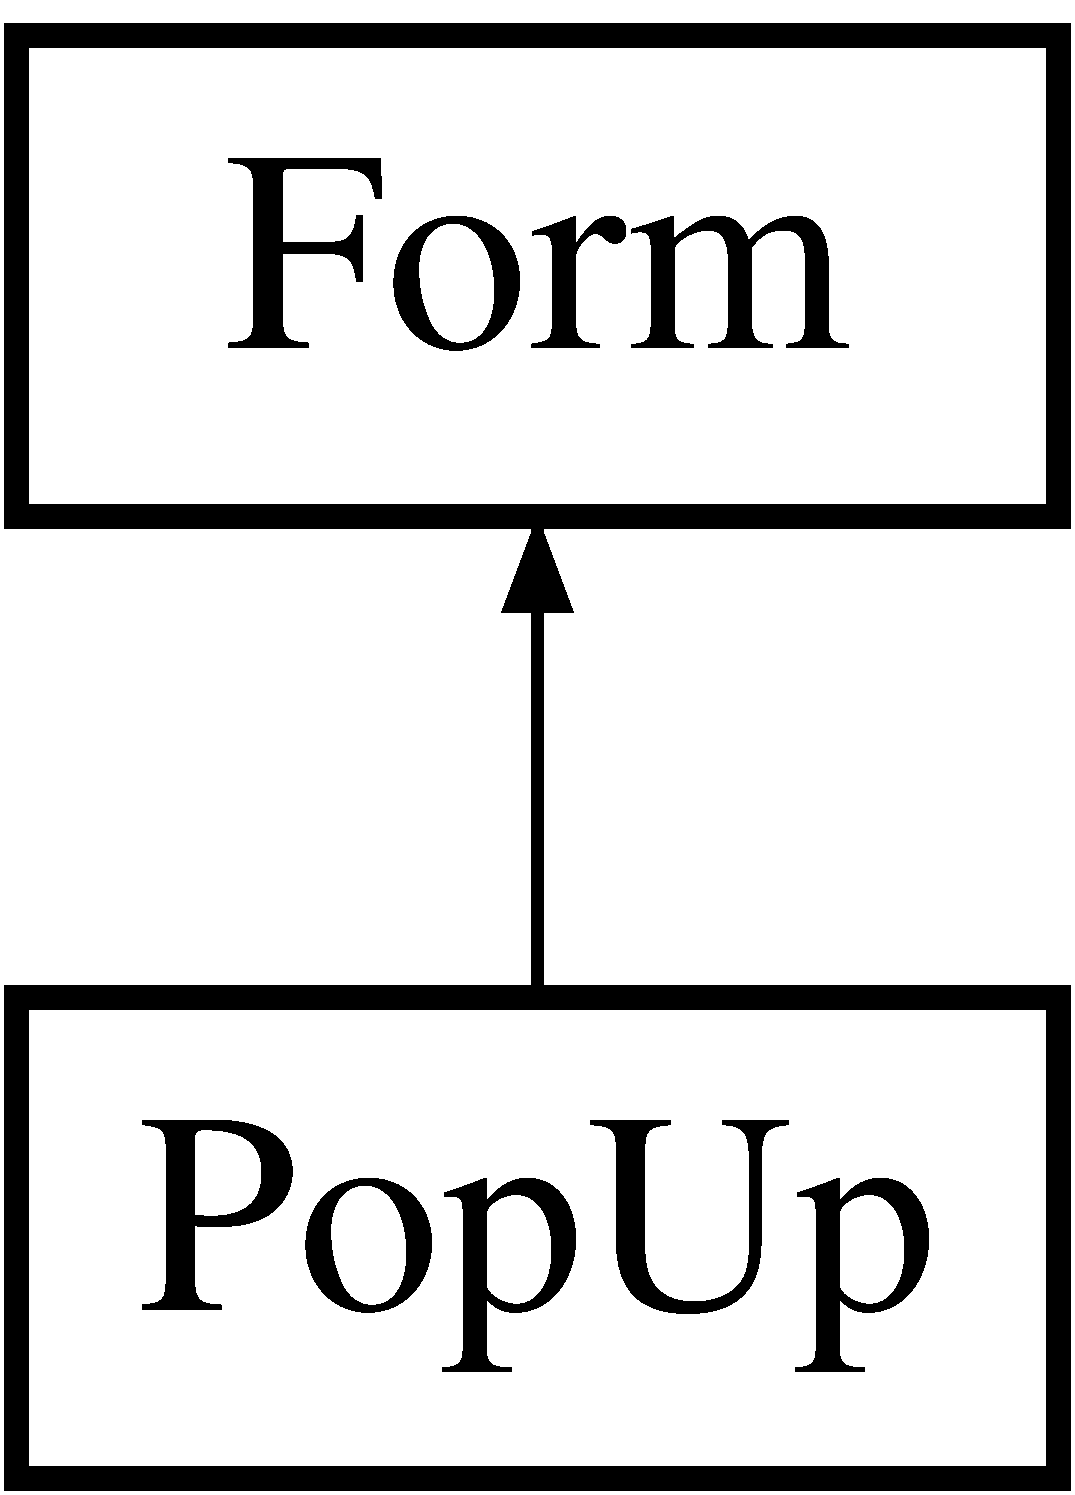
\includegraphics[height=2.000000cm]{classWildlifeTrackingApp_1_1PopUp}
\end{center}
\end{figure}
\subsection*{Public Member Functions}
\begin{DoxyCompactItemize}
\item 
\hyperlink{classWildlifeTrackingApp_1_1PopUp_a67d49d569e4da9c09f0d9b54c3987275}{Pop\+Up} (string message)
\end{DoxyCompactItemize}
\subsection*{Protected Member Functions}
\begin{DoxyCompactItemize}
\item 
override void \hyperlink{classWildlifeTrackingApp_1_1PopUp_a849c3c7f8d08104f0cdb46bee9fe6389}{Dispose} (bool disposing)
\begin{DoxyCompactList}\small\item\em Clean up any resources being used. \end{DoxyCompactList}\end{DoxyCompactItemize}
\subsection*{Properties}
\begin{DoxyCompactItemize}
\item 
static log4net.\+I\+Log \hyperlink{classWildlifeTrackingApp_1_1PopUp_a5fc9abb86e6110ecd61d0a1a7d740a8a}{Log}\hspace{0.3cm}{\ttfamily  \mbox{[}get, private set\mbox{]}}
\end{DoxyCompactItemize}
\subsection*{Private Member Functions}
\begin{DoxyCompactItemize}
\item 
void \hyperlink{classWildlifeTrackingApp_1_1PopUp_a6405d5db675d5338663195a4d12b4c9f}{Initialize\+Component} ()
\begin{DoxyCompactList}\small\item\em Required method for Designer support -\/ do not modify the contents of this method with the code editor. \end{DoxyCompactList}\item 
void \hyperlink{classWildlifeTrackingApp_1_1PopUp_aacb4f2fe113c4f620d97ffae6a93d313}{ok\+\_\+button\+\_\+\+Click} (object sender, Event\+Args e)
\begin{DoxyCompactList}\small\item\em Event handler for the Ok button click of pop up. \end{DoxyCompactList}\end{DoxyCompactItemize}
\subsection*{Private Attributes}
\begin{DoxyCompactItemize}
\item 
System.\+Component\+Model.\+I\+Container \hyperlink{classWildlifeTrackingApp_1_1PopUp_a02595f1c09713bb71dcb2fbbfc7ffa4b}{components} = null
\begin{DoxyCompactList}\small\item\em Required designer variable. \end{DoxyCompactList}\item 
System.\+Windows.\+Forms.\+Button \hyperlink{classWildlifeTrackingApp_1_1PopUp_acf8fb040918df446cb67b4a46855c4bc}{ok\+\_\+button}
\item 
System.\+Windows.\+Forms.\+Label \hyperlink{classWildlifeTrackingApp_1_1PopUp_a380f8b00794cde9d42ecbee01b0376fa}{pop\+Up\+\_\+label}
\end{DoxyCompactItemize}
\subsection*{Static Private Attributes}
\begin{DoxyCompactItemize}
\item 
static readonly log4net.\+I\+Log \hyperlink{classWildlifeTrackingApp_1_1PopUp_ae6c6142b8525b2f4ac6ee6e003b3106f}{log}
\end{DoxyCompactItemize}


\subsection{Detailed Description}
Form class for showing pop ups. 



\subsection{Constructor \& Destructor Documentation}
\mbox{\Hypertarget{classWildlifeTrackingApp_1_1PopUp_a67d49d569e4da9c09f0d9b54c3987275}\label{classWildlifeTrackingApp_1_1PopUp_a67d49d569e4da9c09f0d9b54c3987275}} 
\index{Wildlife\+Tracking\+App\+::\+Pop\+Up@{Wildlife\+Tracking\+App\+::\+Pop\+Up}!Pop\+Up@{Pop\+Up}}
\index{Pop\+Up@{Pop\+Up}!Wildlife\+Tracking\+App\+::\+Pop\+Up@{Wildlife\+Tracking\+App\+::\+Pop\+Up}}
\subsubsection{\texorpdfstring{Pop\+Up()}{PopUp()}}
{\footnotesize\ttfamily \hyperlink{classWildlifeTrackingApp_1_1PopUp}{Pop\+Up} (\begin{DoxyParamCaption}\item[{string}]{message }\end{DoxyParamCaption})\hspace{0.3cm}{\ttfamily [inline]}}



\subsection{Member Function Documentation}
\mbox{\Hypertarget{classWildlifeTrackingApp_1_1PopUp_a849c3c7f8d08104f0cdb46bee9fe6389}\label{classWildlifeTrackingApp_1_1PopUp_a849c3c7f8d08104f0cdb46bee9fe6389}} 
\index{Wildlife\+Tracking\+App\+::\+Pop\+Up@{Wildlife\+Tracking\+App\+::\+Pop\+Up}!Dispose@{Dispose}}
\index{Dispose@{Dispose}!Wildlife\+Tracking\+App\+::\+Pop\+Up@{Wildlife\+Tracking\+App\+::\+Pop\+Up}}
\subsubsection{\texorpdfstring{Dispose()}{Dispose()}}
{\footnotesize\ttfamily override void Dispose (\begin{DoxyParamCaption}\item[{bool}]{disposing }\end{DoxyParamCaption})\hspace{0.3cm}{\ttfamily [inline]}, {\ttfamily [protected]}}



Clean up any resources being used. 


\begin{DoxyParams}{Parameters}
{\em disposing} & true if managed resources should be disposed; otherwise, false.\\
\hline
\end{DoxyParams}
\mbox{\Hypertarget{classWildlifeTrackingApp_1_1PopUp_a6405d5db675d5338663195a4d12b4c9f}\label{classWildlifeTrackingApp_1_1PopUp_a6405d5db675d5338663195a4d12b4c9f}} 
\index{Wildlife\+Tracking\+App\+::\+Pop\+Up@{Wildlife\+Tracking\+App\+::\+Pop\+Up}!Initialize\+Component@{Initialize\+Component}}
\index{Initialize\+Component@{Initialize\+Component}!Wildlife\+Tracking\+App\+::\+Pop\+Up@{Wildlife\+Tracking\+App\+::\+Pop\+Up}}
\subsubsection{\texorpdfstring{Initialize\+Component()}{InitializeComponent()}}
{\footnotesize\ttfamily void Initialize\+Component (\begin{DoxyParamCaption}{ }\end{DoxyParamCaption})\hspace{0.3cm}{\ttfamily [inline]}, {\ttfamily [private]}}



Required method for Designer support -\/ do not modify the contents of this method with the code editor. 

\mbox{\Hypertarget{classWildlifeTrackingApp_1_1PopUp_aacb4f2fe113c4f620d97ffae6a93d313}\label{classWildlifeTrackingApp_1_1PopUp_aacb4f2fe113c4f620d97ffae6a93d313}} 
\index{Wildlife\+Tracking\+App\+::\+Pop\+Up@{Wildlife\+Tracking\+App\+::\+Pop\+Up}!ok\+\_\+button\+\_\+\+Click@{ok\+\_\+button\+\_\+\+Click}}
\index{ok\+\_\+button\+\_\+\+Click@{ok\+\_\+button\+\_\+\+Click}!Wildlife\+Tracking\+App\+::\+Pop\+Up@{Wildlife\+Tracking\+App\+::\+Pop\+Up}}
\subsubsection{\texorpdfstring{ok\+\_\+button\+\_\+\+Click()}{ok\_button\_Click()}}
{\footnotesize\ttfamily void ok\+\_\+button\+\_\+\+Click (\begin{DoxyParamCaption}\item[{object}]{sender,  }\item[{Event\+Args}]{e }\end{DoxyParamCaption})\hspace{0.3cm}{\ttfamily [inline]}, {\ttfamily [private]}}



Event handler for the Ok button click of pop up. 


\begin{DoxyParams}{Parameters}
{\em sender} & Sender Object\\
\hline
{\em e} & Event argument\\
\hline
\end{DoxyParams}


\subsection{Member Data Documentation}
\mbox{\Hypertarget{classWildlifeTrackingApp_1_1PopUp_a02595f1c09713bb71dcb2fbbfc7ffa4b}\label{classWildlifeTrackingApp_1_1PopUp_a02595f1c09713bb71dcb2fbbfc7ffa4b}} 
\index{Wildlife\+Tracking\+App\+::\+Pop\+Up@{Wildlife\+Tracking\+App\+::\+Pop\+Up}!components@{components}}
\index{components@{components}!Wildlife\+Tracking\+App\+::\+Pop\+Up@{Wildlife\+Tracking\+App\+::\+Pop\+Up}}
\subsubsection{\texorpdfstring{components}{components}}
{\footnotesize\ttfamily System.\+Component\+Model.\+I\+Container components = null\hspace{0.3cm}{\ttfamily [private]}}



Required designer variable. 

\mbox{\Hypertarget{classWildlifeTrackingApp_1_1PopUp_ae6c6142b8525b2f4ac6ee6e003b3106f}\label{classWildlifeTrackingApp_1_1PopUp_ae6c6142b8525b2f4ac6ee6e003b3106f}} 
\index{Wildlife\+Tracking\+App\+::\+Pop\+Up@{Wildlife\+Tracking\+App\+::\+Pop\+Up}!log@{log}}
\index{log@{log}!Wildlife\+Tracking\+App\+::\+Pop\+Up@{Wildlife\+Tracking\+App\+::\+Pop\+Up}}
\subsubsection{\texorpdfstring{log}{log}}
{\footnotesize\ttfamily readonly log4net.\+I\+Log log\hspace{0.3cm}{\ttfamily [static]}, {\ttfamily [private]}}

{\bfseries Initial value\+:}
\begin{DoxyCode}
= log4net.LogManager.GetLogger
        (\hyperlink{namespaceSystem}{System}.Reflection.MethodBase.GetCurrentMethod().DeclaringType)
\end{DoxyCode}
\mbox{\Hypertarget{classWildlifeTrackingApp_1_1PopUp_acf8fb040918df446cb67b4a46855c4bc}\label{classWildlifeTrackingApp_1_1PopUp_acf8fb040918df446cb67b4a46855c4bc}} 
\index{Wildlife\+Tracking\+App\+::\+Pop\+Up@{Wildlife\+Tracking\+App\+::\+Pop\+Up}!ok\+\_\+button@{ok\+\_\+button}}
\index{ok\+\_\+button@{ok\+\_\+button}!Wildlife\+Tracking\+App\+::\+Pop\+Up@{Wildlife\+Tracking\+App\+::\+Pop\+Up}}
\subsubsection{\texorpdfstring{ok\+\_\+button}{ok\_button}}
{\footnotesize\ttfamily System.\+Windows.\+Forms.\+Button ok\+\_\+button\hspace{0.3cm}{\ttfamily [private]}}

\mbox{\Hypertarget{classWildlifeTrackingApp_1_1PopUp_a380f8b00794cde9d42ecbee01b0376fa}\label{classWildlifeTrackingApp_1_1PopUp_a380f8b00794cde9d42ecbee01b0376fa}} 
\index{Wildlife\+Tracking\+App\+::\+Pop\+Up@{Wildlife\+Tracking\+App\+::\+Pop\+Up}!pop\+Up\+\_\+label@{pop\+Up\+\_\+label}}
\index{pop\+Up\+\_\+label@{pop\+Up\+\_\+label}!Wildlife\+Tracking\+App\+::\+Pop\+Up@{Wildlife\+Tracking\+App\+::\+Pop\+Up}}
\subsubsection{\texorpdfstring{pop\+Up\+\_\+label}{popUp\_label}}
{\footnotesize\ttfamily System.\+Windows.\+Forms.\+Label pop\+Up\+\_\+label\hspace{0.3cm}{\ttfamily [private]}}



\subsection{Property Documentation}
\mbox{\Hypertarget{classWildlifeTrackingApp_1_1PopUp_a5fc9abb86e6110ecd61d0a1a7d740a8a}\label{classWildlifeTrackingApp_1_1PopUp_a5fc9abb86e6110ecd61d0a1a7d740a8a}} 
\index{Wildlife\+Tracking\+App\+::\+Pop\+Up@{Wildlife\+Tracking\+App\+::\+Pop\+Up}!Log@{Log}}
\index{Log@{Log}!Wildlife\+Tracking\+App\+::\+Pop\+Up@{Wildlife\+Tracking\+App\+::\+Pop\+Up}}
\subsubsection{\texorpdfstring{Log}{Log}}
{\footnotesize\ttfamily log4net.\+I\+Log Log\hspace{0.3cm}{\ttfamily [static]}, {\ttfamily [get]}, {\ttfamily [private set]}}



The documentation for this class was generated from the following files\+:\begin{DoxyCompactItemize}
\item 
View/\hyperlink{PopUp_8cs}{Pop\+Up.\+cs}\item 
View/\hyperlink{PopUp_8Designer_8cs}{Pop\+Up.\+Designer.\+cs}\end{DoxyCompactItemize}

\hypertarget{classWildlifeTrackingApp_1_1Program}{}\section{Program}
\label{classWildlifeTrackingApp_1_1Program}\index{Program@{Program}}
\subsection*{Static Private Member Functions}
\begin{DoxyCompactItemize}
\item 
static void \hyperlink{classWildlifeTrackingApp_1_1Program_a2e67222db1dca5be5f3731ada487dd0f}{Main} ()
\begin{DoxyCompactList}\small\item\em The main entry point for the application. \end{DoxyCompactList}\end{DoxyCompactItemize}


\subsection{Member Function Documentation}
\mbox{\Hypertarget{classWildlifeTrackingApp_1_1Program_a2e67222db1dca5be5f3731ada487dd0f}\label{classWildlifeTrackingApp_1_1Program_a2e67222db1dca5be5f3731ada487dd0f}} 
\index{Wildlife\+Tracking\+App\+::\+Program@{Wildlife\+Tracking\+App\+::\+Program}!Main@{Main}}
\index{Main@{Main}!Wildlife\+Tracking\+App\+::\+Program@{Wildlife\+Tracking\+App\+::\+Program}}
\subsubsection{\texorpdfstring{Main()}{Main()}}
{\footnotesize\ttfamily static void Main (\begin{DoxyParamCaption}{ }\end{DoxyParamCaption})\hspace{0.3cm}{\ttfamily [inline]}, {\ttfamily [static]}, {\ttfamily [private]}}



The main entry point for the application. 



The documentation for this class was generated from the following file\+:\begin{DoxyCompactItemize}
\item 
\hyperlink{Program_8cs}{Program.\+cs}\end{DoxyCompactItemize}

\hypertarget{classWildlifeTrackingApp_1_1Properties_1_1Resources}{}\section{Resources}
\label{classWildlifeTrackingApp_1_1Properties_1_1Resources}\index{Resources@{Resources}}


A strongly-\/typed resource class, for looking up localized strings, etc.  


\subsection*{Package Functions}
\begin{DoxyCompactItemize}
\item 
\hyperlink{classWildlifeTrackingApp_1_1Properties_1_1Resources_aa240237f3113fca394c94bb8a463429f}{Resources} ()
\end{DoxyCompactItemize}
\subsection*{Properties}
\begin{DoxyCompactItemize}
\item 
static global\+::\+System.\+Globalization.\+Culture\+Info \hyperlink{classWildlifeTrackingApp_1_1Properties_1_1Resources_a97174a2d0af83f0bd014787ac18be56c}{Culture}\hspace{0.3cm}{\ttfamily  \mbox{[}get, set\mbox{]}}
\begin{DoxyCompactList}\small\item\em Overrides the current thread\textquotesingle{}s Current\+U\+I\+Culture property for all resource lookups using this strongly typed resource class. \end{DoxyCompactList}\item 
static System.\+Drawing.\+Bitmap \hyperlink{classWildlifeTrackingApp_1_1Properties_1_1Resources_a15aed0ef2486e45a469e5dbf88bce9c4}{do\+\_\+sharp}\hspace{0.3cm}{\ttfamily  \mbox{[}get\mbox{]}}
\begin{DoxyCompactList}\small\item\em Looks up a localized resource of type System.\+Drawing.\+Bitmap. \end{DoxyCompactList}\item 
static System.\+Drawing.\+Bitmap \hyperlink{classWildlifeTrackingApp_1_1Properties_1_1Resources_ad3bb29ee465ca7fd713688ed4e7dbf16}{do\+\_\+sharp1}\hspace{0.3cm}{\ttfamily  \mbox{[}get\mbox{]}}
\begin{DoxyCompactList}\small\item\em Looks up a localized resource of type System.\+Drawing.\+Bitmap. \end{DoxyCompactList}\item 
static System.\+Drawing.\+Bitmap \hyperlink{classWildlifeTrackingApp_1_1Properties_1_1Resources_af2008514522aed5e1ed9d40c4dec4c6b}{do\+\_\+sharp2}\hspace{0.3cm}{\ttfamily  \mbox{[}get\mbox{]}}
\begin{DoxyCompactList}\small\item\em Looks up a localized resource of type System.\+Drawing.\+Bitmap. \end{DoxyCompactList}\item 
static System.\+Drawing.\+Bitmap \hyperlink{classWildlifeTrackingApp_1_1Properties_1_1Resources_af4364b8861b665b628d538a18d818fbd}{do\+\_\+sharp\+OR}\hspace{0.3cm}{\ttfamily  \mbox{[}get\mbox{]}}
\begin{DoxyCompactList}\small\item\em Looks up a localized resource of type System.\+Drawing.\+Bitmap. \end{DoxyCompactList}\item 
static System.\+Drawing.\+Bitmap \hyperlink{classWildlifeTrackingApp_1_1Properties_1_1Resources_ab919b7600d84247495b540af2c9f92be}{do\+\_\+sharp\+O\+R1}\hspace{0.3cm}{\ttfamily  \mbox{[}get\mbox{]}}
\begin{DoxyCompactList}\small\item\em Looks up a localized resource of type System.\+Drawing.\+Bitmap. \end{DoxyCompactList}\item 
static System.\+Drawing.\+Bitmap \hyperlink{classWildlifeTrackingApp_1_1Properties_1_1Resources_ac755af249e0731fb7bc6227eeebf5f1e}{DP}\hspace{0.3cm}{\ttfamily  \mbox{[}get\mbox{]}}
\begin{DoxyCompactList}\small\item\em Looks up a localized resource of type System.\+Drawing.\+Bitmap. \end{DoxyCompactList}\item 
static System.\+Drawing.\+Bitmap \hyperlink{classWildlifeTrackingApp_1_1Properties_1_1Resources_a103bcf459cf832b2c7b9d9a7c5ffb55e}{green}\hspace{0.3cm}{\ttfamily  \mbox{[}get\mbox{]}}
\begin{DoxyCompactList}\small\item\em Looks up a localized resource of type System.\+Drawing.\+Bitmap. \end{DoxyCompactList}\item 
static System.\+Drawing.\+Bitmap \hyperlink{classWildlifeTrackingApp_1_1Properties_1_1Resources_ada97aa4495af0cb5098a56ffbf0f858d}{leaf}\hspace{0.3cm}{\ttfamily  \mbox{[}get\mbox{]}}
\begin{DoxyCompactList}\small\item\em Looks up a localized resource of type System.\+Drawing.\+Bitmap. \end{DoxyCompactList}\item 
static System.\+Drawing.\+Bitmap \hyperlink{classWildlifeTrackingApp_1_1Properties_1_1Resources_adec538f2d25807e5bde6e710a7ba6204}{leaf1}\hspace{0.3cm}{\ttfamily  \mbox{[}get\mbox{]}}
\begin{DoxyCompactList}\small\item\em Looks up a localized resource of type System.\+Drawing.\+Bitmap. \end{DoxyCompactList}\item 
static System.\+Drawing.\+Bitmap \hyperlink{classWildlifeTrackingApp_1_1Properties_1_1Resources_a9d50b18360e8349f940ae5562791c430}{light\+\_\+green}\hspace{0.3cm}{\ttfamily  \mbox{[}get\mbox{]}}
\begin{DoxyCompactList}\small\item\em Looks up a localized resource of type System.\+Drawing.\+Bitmap. \end{DoxyCompactList}\item 
static System.\+Drawing.\+Bitmap \hyperlink{classWildlifeTrackingApp_1_1Properties_1_1Resources_abb170f035e4e40293fc18a5ae75104c0}{light\+\_\+green\+\_\+background\+\_\+2}\hspace{0.3cm}{\ttfamily  \mbox{[}get\mbox{]}}
\begin{DoxyCompactList}\small\item\em Looks up a localized resource of type System.\+Drawing.\+Bitmap. \end{DoxyCompactList}\item 
static System.\+Drawing.\+Bitmap \hyperlink{classWildlifeTrackingApp_1_1Properties_1_1Resources_a22fc764559548610cceff5de0437f793}{par}\hspace{0.3cm}{\ttfamily  \mbox{[}get\mbox{]}}
\begin{DoxyCompactList}\small\item\em Looks up a localized resource of type System.\+Drawing.\+Bitmap. \end{DoxyCompactList}\item 
static System.\+Drawing.\+Bitmap \hyperlink{classWildlifeTrackingApp_1_1Properties_1_1Resources_a08e964ce4a55697ad449abbceae82448}{P\+A\+R\+E\+D\+I\+T\+ED}\hspace{0.3cm}{\ttfamily  \mbox{[}get\mbox{]}}
\begin{DoxyCompactList}\small\item\em Looks up a localized resource of type System.\+Drawing.\+Bitmap. \end{DoxyCompactList}\item 
static System.\+Drawing.\+Bitmap \hyperlink{classWildlifeTrackingApp_1_1Properties_1_1Resources_a515412ebae6fcb28be00cd8faa02bc4d}{plain}\hspace{0.3cm}{\ttfamily  \mbox{[}get\mbox{]}}
\begin{DoxyCompactList}\small\item\em Looks up a localized resource of type System.\+Drawing.\+Bitmap. \end{DoxyCompactList}\item 
static global\+::\+System.\+Resources.\+Resource\+Manager \hyperlink{classWildlifeTrackingApp_1_1Properties_1_1Resources_a0facd9f93017f922ba97bef37fd95b1d}{Resource\+Manager}\hspace{0.3cm}{\ttfamily  \mbox{[}get\mbox{]}}
\begin{DoxyCompactList}\small\item\em Returns the cached Resource\+Manager instance used by this class. \end{DoxyCompactList}\item 
static System.\+Drawing.\+Bitmap \hyperlink{classWildlifeTrackingApp_1_1Properties_1_1Resources_a1c8ec9f550bb1f3cbe7cc93257b0b4d7}{tiger}\hspace{0.3cm}{\ttfamily  \mbox{[}get\mbox{]}}
\begin{DoxyCompactList}\small\item\em Looks up a localized resource of type System.\+Drawing.\+Bitmap. \end{DoxyCompactList}\item 
static System.\+Drawing.\+Bitmap \hyperlink{classWildlifeTrackingApp_1_1Properties_1_1Resources_a0f99bbab5f157297954b10d71ba7d26e}{w1}\hspace{0.3cm}{\ttfamily  \mbox{[}get\mbox{]}}
\begin{DoxyCompactList}\small\item\em Looks up a localized resource of type System.\+Drawing.\+Bitmap. \end{DoxyCompactList}\item 
static System.\+Drawing.\+Bitmap \hyperlink{classWildlifeTrackingApp_1_1Properties_1_1Resources_adae137008920fbb97e674cf1b3af8c1c}{w3}\hspace{0.3cm}{\ttfamily  \mbox{[}get\mbox{]}}
\begin{DoxyCompactList}\small\item\em Looks up a localized resource of type System.\+Drawing.\+Bitmap. \end{DoxyCompactList}\item 
static System.\+Drawing.\+Bitmap \hyperlink{classWildlifeTrackingApp_1_1Properties_1_1Resources_ad53def0f8b6789aa31ac53fda40bbac5}{Xf\+L7\+I5}\hspace{0.3cm}{\ttfamily  \mbox{[}get\mbox{]}}
\begin{DoxyCompactList}\small\item\em Looks up a localized resource of type System.\+Drawing.\+Bitmap. \end{DoxyCompactList}\item 
static System.\+Drawing.\+Bitmap \hyperlink{classWildlifeTrackingApp_1_1Properties_1_1Resources_af61d1311106833aa651ee30943901e17}{Xf\+L7\+I51}\hspace{0.3cm}{\ttfamily  \mbox{[}get\mbox{]}}
\begin{DoxyCompactList}\small\item\em Looks up a localized resource of type System.\+Drawing.\+Bitmap. \end{DoxyCompactList}\end{DoxyCompactItemize}
\subsection*{Static Private Attributes}
\begin{DoxyCompactItemize}
\item 
static global\+::\+System.\+Globalization.\+Culture\+Info \hyperlink{classWildlifeTrackingApp_1_1Properties_1_1Resources_a87058a34a8b44628f03942ac02c08560}{resource\+Culture}
\item 
static global\+::\+System.\+Resources.\+Resource\+Manager \hyperlink{classWildlifeTrackingApp_1_1Properties_1_1Resources_a5a5d416265010ce4273651e495fda152}{resource\+Man}
\end{DoxyCompactItemize}


\subsection{Detailed Description}
A strongly-\/typed resource class, for looking up localized strings, etc. 



\subsection{Constructor \& Destructor Documentation}
\mbox{\Hypertarget{classWildlifeTrackingApp_1_1Properties_1_1Resources_aa240237f3113fca394c94bb8a463429f}\label{classWildlifeTrackingApp_1_1Properties_1_1Resources_aa240237f3113fca394c94bb8a463429f}} 
\index{Wildlife\+Tracking\+App\+::\+Properties\+::\+Resources@{Wildlife\+Tracking\+App\+::\+Properties\+::\+Resources}!Resources@{Resources}}
\index{Resources@{Resources}!Wildlife\+Tracking\+App\+::\+Properties\+::\+Resources@{Wildlife\+Tracking\+App\+::\+Properties\+::\+Resources}}
\subsubsection{\texorpdfstring{Resources()}{Resources()}}
{\footnotesize\ttfamily \hyperlink{classWildlifeTrackingApp_1_1Properties_1_1Resources}{Resources} (\begin{DoxyParamCaption}{ }\end{DoxyParamCaption})\hspace{0.3cm}{\ttfamily [inline]}, {\ttfamily [package]}}



\subsection{Member Data Documentation}
\mbox{\Hypertarget{classWildlifeTrackingApp_1_1Properties_1_1Resources_a87058a34a8b44628f03942ac02c08560}\label{classWildlifeTrackingApp_1_1Properties_1_1Resources_a87058a34a8b44628f03942ac02c08560}} 
\index{Wildlife\+Tracking\+App\+::\+Properties\+::\+Resources@{Wildlife\+Tracking\+App\+::\+Properties\+::\+Resources}!resource\+Culture@{resource\+Culture}}
\index{resource\+Culture@{resource\+Culture}!Wildlife\+Tracking\+App\+::\+Properties\+::\+Resources@{Wildlife\+Tracking\+App\+::\+Properties\+::\+Resources}}
\subsubsection{\texorpdfstring{resource\+Culture}{resourceCulture}}
{\footnotesize\ttfamily global.\+System.\+Globalization.\+Culture\+Info resource\+Culture\hspace{0.3cm}{\ttfamily [static]}, {\ttfamily [private]}}

\mbox{\Hypertarget{classWildlifeTrackingApp_1_1Properties_1_1Resources_a5a5d416265010ce4273651e495fda152}\label{classWildlifeTrackingApp_1_1Properties_1_1Resources_a5a5d416265010ce4273651e495fda152}} 
\index{Wildlife\+Tracking\+App\+::\+Properties\+::\+Resources@{Wildlife\+Tracking\+App\+::\+Properties\+::\+Resources}!resource\+Man@{resource\+Man}}
\index{resource\+Man@{resource\+Man}!Wildlife\+Tracking\+App\+::\+Properties\+::\+Resources@{Wildlife\+Tracking\+App\+::\+Properties\+::\+Resources}}
\subsubsection{\texorpdfstring{resource\+Man}{resourceMan}}
{\footnotesize\ttfamily global.\+System.\+Resources.\+Resource\+Manager resource\+Man\hspace{0.3cm}{\ttfamily [static]}, {\ttfamily [private]}}



\subsection{Property Documentation}
\mbox{\Hypertarget{classWildlifeTrackingApp_1_1Properties_1_1Resources_a97174a2d0af83f0bd014787ac18be56c}\label{classWildlifeTrackingApp_1_1Properties_1_1Resources_a97174a2d0af83f0bd014787ac18be56c}} 
\index{Wildlife\+Tracking\+App\+::\+Properties\+::\+Resources@{Wildlife\+Tracking\+App\+::\+Properties\+::\+Resources}!Culture@{Culture}}
\index{Culture@{Culture}!Wildlife\+Tracking\+App\+::\+Properties\+::\+Resources@{Wildlife\+Tracking\+App\+::\+Properties\+::\+Resources}}
\subsubsection{\texorpdfstring{Culture}{Culture}}
{\footnotesize\ttfamily global.\+System.\+Globalization.\+Culture\+Info Culture\hspace{0.3cm}{\ttfamily [static]}, {\ttfamily [get]}, {\ttfamily [set]}, {\ttfamily [package]}}



Overrides the current thread\textquotesingle{}s Current\+U\+I\+Culture property for all resource lookups using this strongly typed resource class. 

\mbox{\Hypertarget{classWildlifeTrackingApp_1_1Properties_1_1Resources_a15aed0ef2486e45a469e5dbf88bce9c4}\label{classWildlifeTrackingApp_1_1Properties_1_1Resources_a15aed0ef2486e45a469e5dbf88bce9c4}} 
\index{Wildlife\+Tracking\+App\+::\+Properties\+::\+Resources@{Wildlife\+Tracking\+App\+::\+Properties\+::\+Resources}!do\+\_\+sharp@{do\+\_\+sharp}}
\index{do\+\_\+sharp@{do\+\_\+sharp}!Wildlife\+Tracking\+App\+::\+Properties\+::\+Resources@{Wildlife\+Tracking\+App\+::\+Properties\+::\+Resources}}
\subsubsection{\texorpdfstring{do\+\_\+sharp}{do\_sharp}}
{\footnotesize\ttfamily System.\+Drawing.\+Bitmap do\+\_\+sharp\hspace{0.3cm}{\ttfamily [static]}, {\ttfamily [get]}, {\ttfamily [package]}}



Looks up a localized resource of type System.\+Drawing.\+Bitmap. 

\mbox{\Hypertarget{classWildlifeTrackingApp_1_1Properties_1_1Resources_ad3bb29ee465ca7fd713688ed4e7dbf16}\label{classWildlifeTrackingApp_1_1Properties_1_1Resources_ad3bb29ee465ca7fd713688ed4e7dbf16}} 
\index{Wildlife\+Tracking\+App\+::\+Properties\+::\+Resources@{Wildlife\+Tracking\+App\+::\+Properties\+::\+Resources}!do\+\_\+sharp1@{do\+\_\+sharp1}}
\index{do\+\_\+sharp1@{do\+\_\+sharp1}!Wildlife\+Tracking\+App\+::\+Properties\+::\+Resources@{Wildlife\+Tracking\+App\+::\+Properties\+::\+Resources}}
\subsubsection{\texorpdfstring{do\+\_\+sharp1}{do\_sharp1}}
{\footnotesize\ttfamily System.\+Drawing.\+Bitmap do\+\_\+sharp1\hspace{0.3cm}{\ttfamily [static]}, {\ttfamily [get]}, {\ttfamily [package]}}



Looks up a localized resource of type System.\+Drawing.\+Bitmap. 

\mbox{\Hypertarget{classWildlifeTrackingApp_1_1Properties_1_1Resources_af2008514522aed5e1ed9d40c4dec4c6b}\label{classWildlifeTrackingApp_1_1Properties_1_1Resources_af2008514522aed5e1ed9d40c4dec4c6b}} 
\index{Wildlife\+Tracking\+App\+::\+Properties\+::\+Resources@{Wildlife\+Tracking\+App\+::\+Properties\+::\+Resources}!do\+\_\+sharp2@{do\+\_\+sharp2}}
\index{do\+\_\+sharp2@{do\+\_\+sharp2}!Wildlife\+Tracking\+App\+::\+Properties\+::\+Resources@{Wildlife\+Tracking\+App\+::\+Properties\+::\+Resources}}
\subsubsection{\texorpdfstring{do\+\_\+sharp2}{do\_sharp2}}
{\footnotesize\ttfamily System.\+Drawing.\+Bitmap do\+\_\+sharp2\hspace{0.3cm}{\ttfamily [static]}, {\ttfamily [get]}, {\ttfamily [package]}}



Looks up a localized resource of type System.\+Drawing.\+Bitmap. 

\mbox{\Hypertarget{classWildlifeTrackingApp_1_1Properties_1_1Resources_af4364b8861b665b628d538a18d818fbd}\label{classWildlifeTrackingApp_1_1Properties_1_1Resources_af4364b8861b665b628d538a18d818fbd}} 
\index{Wildlife\+Tracking\+App\+::\+Properties\+::\+Resources@{Wildlife\+Tracking\+App\+::\+Properties\+::\+Resources}!do\+\_\+sharp\+OR@{do\+\_\+sharp\+OR}}
\index{do\+\_\+sharp\+OR@{do\+\_\+sharp\+OR}!Wildlife\+Tracking\+App\+::\+Properties\+::\+Resources@{Wildlife\+Tracking\+App\+::\+Properties\+::\+Resources}}
\subsubsection{\texorpdfstring{do\+\_\+sharp\+OR}{do\_sharpOR}}
{\footnotesize\ttfamily System.\+Drawing.\+Bitmap do\+\_\+sharp\+OR\hspace{0.3cm}{\ttfamily [static]}, {\ttfamily [get]}, {\ttfamily [package]}}



Looks up a localized resource of type System.\+Drawing.\+Bitmap. 

\mbox{\Hypertarget{classWildlifeTrackingApp_1_1Properties_1_1Resources_ab919b7600d84247495b540af2c9f92be}\label{classWildlifeTrackingApp_1_1Properties_1_1Resources_ab919b7600d84247495b540af2c9f92be}} 
\index{Wildlife\+Tracking\+App\+::\+Properties\+::\+Resources@{Wildlife\+Tracking\+App\+::\+Properties\+::\+Resources}!do\+\_\+sharp\+O\+R1@{do\+\_\+sharp\+O\+R1}}
\index{do\+\_\+sharp\+O\+R1@{do\+\_\+sharp\+O\+R1}!Wildlife\+Tracking\+App\+::\+Properties\+::\+Resources@{Wildlife\+Tracking\+App\+::\+Properties\+::\+Resources}}
\subsubsection{\texorpdfstring{do\+\_\+sharp\+O\+R1}{do\_sharpOR1}}
{\footnotesize\ttfamily System.\+Drawing.\+Bitmap do\+\_\+sharp\+O\+R1\hspace{0.3cm}{\ttfamily [static]}, {\ttfamily [get]}, {\ttfamily [package]}}



Looks up a localized resource of type System.\+Drawing.\+Bitmap. 

\mbox{\Hypertarget{classWildlifeTrackingApp_1_1Properties_1_1Resources_ac755af249e0731fb7bc6227eeebf5f1e}\label{classWildlifeTrackingApp_1_1Properties_1_1Resources_ac755af249e0731fb7bc6227eeebf5f1e}} 
\index{Wildlife\+Tracking\+App\+::\+Properties\+::\+Resources@{Wildlife\+Tracking\+App\+::\+Properties\+::\+Resources}!DP@{DP}}
\index{DP@{DP}!Wildlife\+Tracking\+App\+::\+Properties\+::\+Resources@{Wildlife\+Tracking\+App\+::\+Properties\+::\+Resources}}
\subsubsection{\texorpdfstring{DP}{DP}}
{\footnotesize\ttfamily System.\+Drawing.\+Bitmap DP\hspace{0.3cm}{\ttfamily [static]}, {\ttfamily [get]}, {\ttfamily [package]}}



Looks up a localized resource of type System.\+Drawing.\+Bitmap. 

\mbox{\Hypertarget{classWildlifeTrackingApp_1_1Properties_1_1Resources_a103bcf459cf832b2c7b9d9a7c5ffb55e}\label{classWildlifeTrackingApp_1_1Properties_1_1Resources_a103bcf459cf832b2c7b9d9a7c5ffb55e}} 
\index{Wildlife\+Tracking\+App\+::\+Properties\+::\+Resources@{Wildlife\+Tracking\+App\+::\+Properties\+::\+Resources}!green@{green}}
\index{green@{green}!Wildlife\+Tracking\+App\+::\+Properties\+::\+Resources@{Wildlife\+Tracking\+App\+::\+Properties\+::\+Resources}}
\subsubsection{\texorpdfstring{green}{green}}
{\footnotesize\ttfamily System.\+Drawing.\+Bitmap green\hspace{0.3cm}{\ttfamily [static]}, {\ttfamily [get]}, {\ttfamily [package]}}



Looks up a localized resource of type System.\+Drawing.\+Bitmap. 

\mbox{\Hypertarget{classWildlifeTrackingApp_1_1Properties_1_1Resources_ada97aa4495af0cb5098a56ffbf0f858d}\label{classWildlifeTrackingApp_1_1Properties_1_1Resources_ada97aa4495af0cb5098a56ffbf0f858d}} 
\index{Wildlife\+Tracking\+App\+::\+Properties\+::\+Resources@{Wildlife\+Tracking\+App\+::\+Properties\+::\+Resources}!leaf@{leaf}}
\index{leaf@{leaf}!Wildlife\+Tracking\+App\+::\+Properties\+::\+Resources@{Wildlife\+Tracking\+App\+::\+Properties\+::\+Resources}}
\subsubsection{\texorpdfstring{leaf}{leaf}}
{\footnotesize\ttfamily System.\+Drawing.\+Bitmap leaf\hspace{0.3cm}{\ttfamily [static]}, {\ttfamily [get]}, {\ttfamily [package]}}



Looks up a localized resource of type System.\+Drawing.\+Bitmap. 

\mbox{\Hypertarget{classWildlifeTrackingApp_1_1Properties_1_1Resources_adec538f2d25807e5bde6e710a7ba6204}\label{classWildlifeTrackingApp_1_1Properties_1_1Resources_adec538f2d25807e5bde6e710a7ba6204}} 
\index{Wildlife\+Tracking\+App\+::\+Properties\+::\+Resources@{Wildlife\+Tracking\+App\+::\+Properties\+::\+Resources}!leaf1@{leaf1}}
\index{leaf1@{leaf1}!Wildlife\+Tracking\+App\+::\+Properties\+::\+Resources@{Wildlife\+Tracking\+App\+::\+Properties\+::\+Resources}}
\subsubsection{\texorpdfstring{leaf1}{leaf1}}
{\footnotesize\ttfamily System.\+Drawing.\+Bitmap leaf1\hspace{0.3cm}{\ttfamily [static]}, {\ttfamily [get]}, {\ttfamily [package]}}



Looks up a localized resource of type System.\+Drawing.\+Bitmap. 

\mbox{\Hypertarget{classWildlifeTrackingApp_1_1Properties_1_1Resources_a9d50b18360e8349f940ae5562791c430}\label{classWildlifeTrackingApp_1_1Properties_1_1Resources_a9d50b18360e8349f940ae5562791c430}} 
\index{Wildlife\+Tracking\+App\+::\+Properties\+::\+Resources@{Wildlife\+Tracking\+App\+::\+Properties\+::\+Resources}!light\+\_\+green@{light\+\_\+green}}
\index{light\+\_\+green@{light\+\_\+green}!Wildlife\+Tracking\+App\+::\+Properties\+::\+Resources@{Wildlife\+Tracking\+App\+::\+Properties\+::\+Resources}}
\subsubsection{\texorpdfstring{light\+\_\+green}{light\_green}}
{\footnotesize\ttfamily System.\+Drawing.\+Bitmap light\+\_\+green\hspace{0.3cm}{\ttfamily [static]}, {\ttfamily [get]}, {\ttfamily [package]}}



Looks up a localized resource of type System.\+Drawing.\+Bitmap. 

\mbox{\Hypertarget{classWildlifeTrackingApp_1_1Properties_1_1Resources_abb170f035e4e40293fc18a5ae75104c0}\label{classWildlifeTrackingApp_1_1Properties_1_1Resources_abb170f035e4e40293fc18a5ae75104c0}} 
\index{Wildlife\+Tracking\+App\+::\+Properties\+::\+Resources@{Wildlife\+Tracking\+App\+::\+Properties\+::\+Resources}!light\+\_\+green\+\_\+background\+\_\+2@{light\+\_\+green\+\_\+background\+\_\+2}}
\index{light\+\_\+green\+\_\+background\+\_\+2@{light\+\_\+green\+\_\+background\+\_\+2}!Wildlife\+Tracking\+App\+::\+Properties\+::\+Resources@{Wildlife\+Tracking\+App\+::\+Properties\+::\+Resources}}
\subsubsection{\texorpdfstring{light\+\_\+green\+\_\+background\+\_\+2}{light\_green\_background\_2}}
{\footnotesize\ttfamily System.\+Drawing.\+Bitmap light\+\_\+green\+\_\+background\+\_\+2\hspace{0.3cm}{\ttfamily [static]}, {\ttfamily [get]}, {\ttfamily [package]}}



Looks up a localized resource of type System.\+Drawing.\+Bitmap. 

\mbox{\Hypertarget{classWildlifeTrackingApp_1_1Properties_1_1Resources_a22fc764559548610cceff5de0437f793}\label{classWildlifeTrackingApp_1_1Properties_1_1Resources_a22fc764559548610cceff5de0437f793}} 
\index{Wildlife\+Tracking\+App\+::\+Properties\+::\+Resources@{Wildlife\+Tracking\+App\+::\+Properties\+::\+Resources}!par@{par}}
\index{par@{par}!Wildlife\+Tracking\+App\+::\+Properties\+::\+Resources@{Wildlife\+Tracking\+App\+::\+Properties\+::\+Resources}}
\subsubsection{\texorpdfstring{par}{par}}
{\footnotesize\ttfamily System.\+Drawing.\+Bitmap par\hspace{0.3cm}{\ttfamily [static]}, {\ttfamily [get]}, {\ttfamily [package]}}



Looks up a localized resource of type System.\+Drawing.\+Bitmap. 

\mbox{\Hypertarget{classWildlifeTrackingApp_1_1Properties_1_1Resources_a08e964ce4a55697ad449abbceae82448}\label{classWildlifeTrackingApp_1_1Properties_1_1Resources_a08e964ce4a55697ad449abbceae82448}} 
\index{Wildlife\+Tracking\+App\+::\+Properties\+::\+Resources@{Wildlife\+Tracking\+App\+::\+Properties\+::\+Resources}!P\+A\+R\+E\+D\+I\+T\+ED@{P\+A\+R\+E\+D\+I\+T\+ED}}
\index{P\+A\+R\+E\+D\+I\+T\+ED@{P\+A\+R\+E\+D\+I\+T\+ED}!Wildlife\+Tracking\+App\+::\+Properties\+::\+Resources@{Wildlife\+Tracking\+App\+::\+Properties\+::\+Resources}}
\subsubsection{\texorpdfstring{P\+A\+R\+E\+D\+I\+T\+ED}{PAREDITED}}
{\footnotesize\ttfamily System.\+Drawing.\+Bitmap P\+A\+R\+E\+D\+I\+T\+ED\hspace{0.3cm}{\ttfamily [static]}, {\ttfamily [get]}, {\ttfamily [package]}}



Looks up a localized resource of type System.\+Drawing.\+Bitmap. 

\mbox{\Hypertarget{classWildlifeTrackingApp_1_1Properties_1_1Resources_a515412ebae6fcb28be00cd8faa02bc4d}\label{classWildlifeTrackingApp_1_1Properties_1_1Resources_a515412ebae6fcb28be00cd8faa02bc4d}} 
\index{Wildlife\+Tracking\+App\+::\+Properties\+::\+Resources@{Wildlife\+Tracking\+App\+::\+Properties\+::\+Resources}!plain@{plain}}
\index{plain@{plain}!Wildlife\+Tracking\+App\+::\+Properties\+::\+Resources@{Wildlife\+Tracking\+App\+::\+Properties\+::\+Resources}}
\subsubsection{\texorpdfstring{plain}{plain}}
{\footnotesize\ttfamily System.\+Drawing.\+Bitmap plain\hspace{0.3cm}{\ttfamily [static]}, {\ttfamily [get]}, {\ttfamily [package]}}



Looks up a localized resource of type System.\+Drawing.\+Bitmap. 

\mbox{\Hypertarget{classWildlifeTrackingApp_1_1Properties_1_1Resources_a0facd9f93017f922ba97bef37fd95b1d}\label{classWildlifeTrackingApp_1_1Properties_1_1Resources_a0facd9f93017f922ba97bef37fd95b1d}} 
\index{Wildlife\+Tracking\+App\+::\+Properties\+::\+Resources@{Wildlife\+Tracking\+App\+::\+Properties\+::\+Resources}!Resource\+Manager@{Resource\+Manager}}
\index{Resource\+Manager@{Resource\+Manager}!Wildlife\+Tracking\+App\+::\+Properties\+::\+Resources@{Wildlife\+Tracking\+App\+::\+Properties\+::\+Resources}}
\subsubsection{\texorpdfstring{Resource\+Manager}{ResourceManager}}
{\footnotesize\ttfamily global.\+System.\+Resources.\+Resource\+Manager Resource\+Manager\hspace{0.3cm}{\ttfamily [static]}, {\ttfamily [get]}, {\ttfamily [package]}}



Returns the cached Resource\+Manager instance used by this class. 

\mbox{\Hypertarget{classWildlifeTrackingApp_1_1Properties_1_1Resources_a1c8ec9f550bb1f3cbe7cc93257b0b4d7}\label{classWildlifeTrackingApp_1_1Properties_1_1Resources_a1c8ec9f550bb1f3cbe7cc93257b0b4d7}} 
\index{Wildlife\+Tracking\+App\+::\+Properties\+::\+Resources@{Wildlife\+Tracking\+App\+::\+Properties\+::\+Resources}!tiger@{tiger}}
\index{tiger@{tiger}!Wildlife\+Tracking\+App\+::\+Properties\+::\+Resources@{Wildlife\+Tracking\+App\+::\+Properties\+::\+Resources}}
\subsubsection{\texorpdfstring{tiger}{tiger}}
{\footnotesize\ttfamily System.\+Drawing.\+Bitmap tiger\hspace{0.3cm}{\ttfamily [static]}, {\ttfamily [get]}, {\ttfamily [package]}}



Looks up a localized resource of type System.\+Drawing.\+Bitmap. 

\mbox{\Hypertarget{classWildlifeTrackingApp_1_1Properties_1_1Resources_a0f99bbab5f157297954b10d71ba7d26e}\label{classWildlifeTrackingApp_1_1Properties_1_1Resources_a0f99bbab5f157297954b10d71ba7d26e}} 
\index{Wildlife\+Tracking\+App\+::\+Properties\+::\+Resources@{Wildlife\+Tracking\+App\+::\+Properties\+::\+Resources}!w1@{w1}}
\index{w1@{w1}!Wildlife\+Tracking\+App\+::\+Properties\+::\+Resources@{Wildlife\+Tracking\+App\+::\+Properties\+::\+Resources}}
\subsubsection{\texorpdfstring{w1}{w1}}
{\footnotesize\ttfamily System.\+Drawing.\+Bitmap w1\hspace{0.3cm}{\ttfamily [static]}, {\ttfamily [get]}, {\ttfamily [package]}}



Looks up a localized resource of type System.\+Drawing.\+Bitmap. 

\mbox{\Hypertarget{classWildlifeTrackingApp_1_1Properties_1_1Resources_adae137008920fbb97e674cf1b3af8c1c}\label{classWildlifeTrackingApp_1_1Properties_1_1Resources_adae137008920fbb97e674cf1b3af8c1c}} 
\index{Wildlife\+Tracking\+App\+::\+Properties\+::\+Resources@{Wildlife\+Tracking\+App\+::\+Properties\+::\+Resources}!w3@{w3}}
\index{w3@{w3}!Wildlife\+Tracking\+App\+::\+Properties\+::\+Resources@{Wildlife\+Tracking\+App\+::\+Properties\+::\+Resources}}
\subsubsection{\texorpdfstring{w3}{w3}}
{\footnotesize\ttfamily System.\+Drawing.\+Bitmap w3\hspace{0.3cm}{\ttfamily [static]}, {\ttfamily [get]}, {\ttfamily [package]}}



Looks up a localized resource of type System.\+Drawing.\+Bitmap. 

\mbox{\Hypertarget{classWildlifeTrackingApp_1_1Properties_1_1Resources_ad53def0f8b6789aa31ac53fda40bbac5}\label{classWildlifeTrackingApp_1_1Properties_1_1Resources_ad53def0f8b6789aa31ac53fda40bbac5}} 
\index{Wildlife\+Tracking\+App\+::\+Properties\+::\+Resources@{Wildlife\+Tracking\+App\+::\+Properties\+::\+Resources}!Xf\+L7\+I5@{Xf\+L7\+I5}}
\index{Xf\+L7\+I5@{Xf\+L7\+I5}!Wildlife\+Tracking\+App\+::\+Properties\+::\+Resources@{Wildlife\+Tracking\+App\+::\+Properties\+::\+Resources}}
\subsubsection{\texorpdfstring{Xf\+L7\+I5}{XfL7I5}}
{\footnotesize\ttfamily System.\+Drawing.\+Bitmap Xf\+L7\+I5\hspace{0.3cm}{\ttfamily [static]}, {\ttfamily [get]}, {\ttfamily [package]}}



Looks up a localized resource of type System.\+Drawing.\+Bitmap. 

\mbox{\Hypertarget{classWildlifeTrackingApp_1_1Properties_1_1Resources_af61d1311106833aa651ee30943901e17}\label{classWildlifeTrackingApp_1_1Properties_1_1Resources_af61d1311106833aa651ee30943901e17}} 
\index{Wildlife\+Tracking\+App\+::\+Properties\+::\+Resources@{Wildlife\+Tracking\+App\+::\+Properties\+::\+Resources}!Xf\+L7\+I51@{Xf\+L7\+I51}}
\index{Xf\+L7\+I51@{Xf\+L7\+I51}!Wildlife\+Tracking\+App\+::\+Properties\+::\+Resources@{Wildlife\+Tracking\+App\+::\+Properties\+::\+Resources}}
\subsubsection{\texorpdfstring{Xf\+L7\+I51}{XfL7I51}}
{\footnotesize\ttfamily System.\+Drawing.\+Bitmap Xf\+L7\+I51\hspace{0.3cm}{\ttfamily [static]}, {\ttfamily [get]}, {\ttfamily [package]}}



Looks up a localized resource of type System.\+Drawing.\+Bitmap. 



The documentation for this class was generated from the following file\+:\begin{DoxyCompactItemize}
\item 
Properties/\hyperlink{Resources_8Designer_8cs}{Resources.\+Designer.\+cs}\end{DoxyCompactItemize}

\hypertarget{classWildlifeTrackingApp_1_1Properties_1_1Settings}{}\section{Settings}
\label{classWildlifeTrackingApp_1_1Properties_1_1Settings}\index{Settings@{Settings}}
Inheritance diagram for Settings\+:\begin{figure}[H]
\begin{center}
\leavevmode
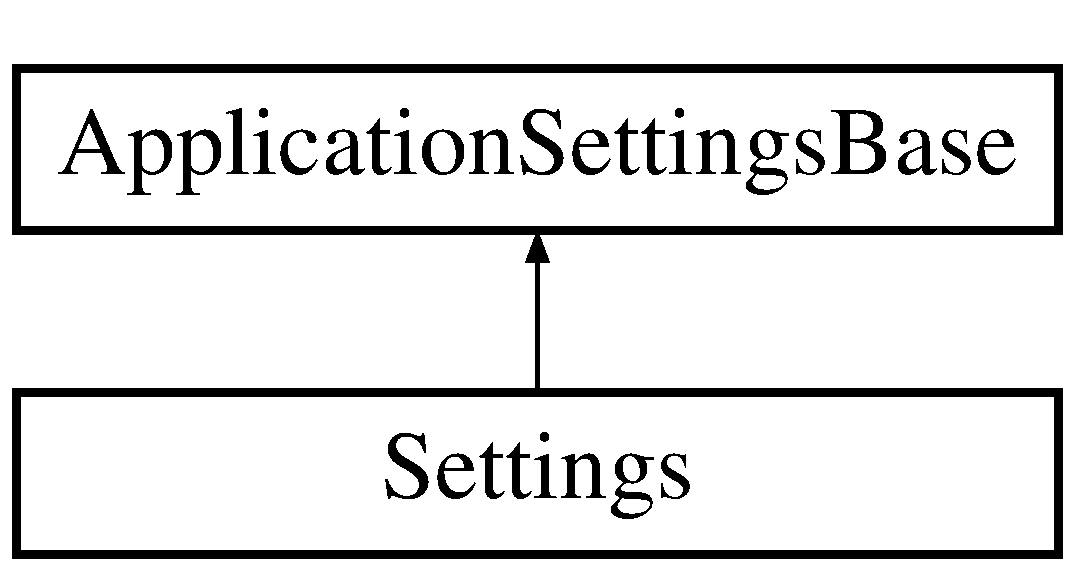
\includegraphics[height=2.000000cm]{classWildlifeTrackingApp_1_1Properties_1_1Settings}
\end{center}
\end{figure}
\subsection*{Properties}
\begin{DoxyCompactItemize}
\item 
static \hyperlink{classWildlifeTrackingApp_1_1Properties_1_1Settings}{Settings} \hyperlink{classWildlifeTrackingApp_1_1Properties_1_1Settings_af44ce680f893da1cfe4575b306835697}{Default}\hspace{0.3cm}{\ttfamily  \mbox{[}get\mbox{]}}
\end{DoxyCompactItemize}
\subsection*{Static Private Attributes}
\begin{DoxyCompactItemize}
\item 
static \hyperlink{classWildlifeTrackingApp_1_1Properties_1_1Settings}{Settings} \hyperlink{classWildlifeTrackingApp_1_1Properties_1_1Settings_a8a09a0578d98ad02e7537e8b01debf7e}{default\+Instance} = ((\hyperlink{classWildlifeTrackingApp_1_1Properties_1_1Settings}{Settings})(global\+::\+System.\+Configuration.\+Application\+Settings\+Base.\+Synchronized(new \hyperlink{classWildlifeTrackingApp_1_1Properties_1_1Settings}{Settings}())))
\end{DoxyCompactItemize}


\subsection{Member Data Documentation}
\mbox{\Hypertarget{classWildlifeTrackingApp_1_1Properties_1_1Settings_a8a09a0578d98ad02e7537e8b01debf7e}\label{classWildlifeTrackingApp_1_1Properties_1_1Settings_a8a09a0578d98ad02e7537e8b01debf7e}} 
\index{Wildlife\+Tracking\+App\+::\+Properties\+::\+Settings@{Wildlife\+Tracking\+App\+::\+Properties\+::\+Settings}!default\+Instance@{default\+Instance}}
\index{default\+Instance@{default\+Instance}!Wildlife\+Tracking\+App\+::\+Properties\+::\+Settings@{Wildlife\+Tracking\+App\+::\+Properties\+::\+Settings}}
\subsubsection{\texorpdfstring{default\+Instance}{defaultInstance}}
{\footnotesize\ttfamily \hyperlink{classWildlifeTrackingApp_1_1Properties_1_1Settings}{Settings} default\+Instance = ((\hyperlink{classWildlifeTrackingApp_1_1Properties_1_1Settings}{Settings})(global\+::\+System.\+Configuration.\+Application\+Settings\+Base.\+Synchronized(new \hyperlink{classWildlifeTrackingApp_1_1Properties_1_1Settings}{Settings}())))\hspace{0.3cm}{\ttfamily [static]}, {\ttfamily [private]}}



\subsection{Property Documentation}
\mbox{\Hypertarget{classWildlifeTrackingApp_1_1Properties_1_1Settings_af44ce680f893da1cfe4575b306835697}\label{classWildlifeTrackingApp_1_1Properties_1_1Settings_af44ce680f893da1cfe4575b306835697}} 
\index{Wildlife\+Tracking\+App\+::\+Properties\+::\+Settings@{Wildlife\+Tracking\+App\+::\+Properties\+::\+Settings}!Default@{Default}}
\index{Default@{Default}!Wildlife\+Tracking\+App\+::\+Properties\+::\+Settings@{Wildlife\+Tracking\+App\+::\+Properties\+::\+Settings}}
\subsubsection{\texorpdfstring{Default}{Default}}
{\footnotesize\ttfamily \hyperlink{classWildlifeTrackingApp_1_1Properties_1_1Settings}{Settings} Default\hspace{0.3cm}{\ttfamily [static]}, {\ttfamily [get]}}



The documentation for this class was generated from the following file\+:\begin{DoxyCompactItemize}
\item 
Properties/\hyperlink{Settings_8Designer_8cs}{Settings.\+Designer.\+cs}\end{DoxyCompactItemize}

\hypertarget{classWildlifeTrackingApp_1_1Report}{}\section{Report}
\label{classWildlifeTrackingApp_1_1Report}\index{Report@{Report}}


Form class for the report generation page. Generates report of total number of animals per categories based on the from and to date.  


Inheritance diagram for Report\+:\begin{figure}[H]
\begin{center}
\leavevmode
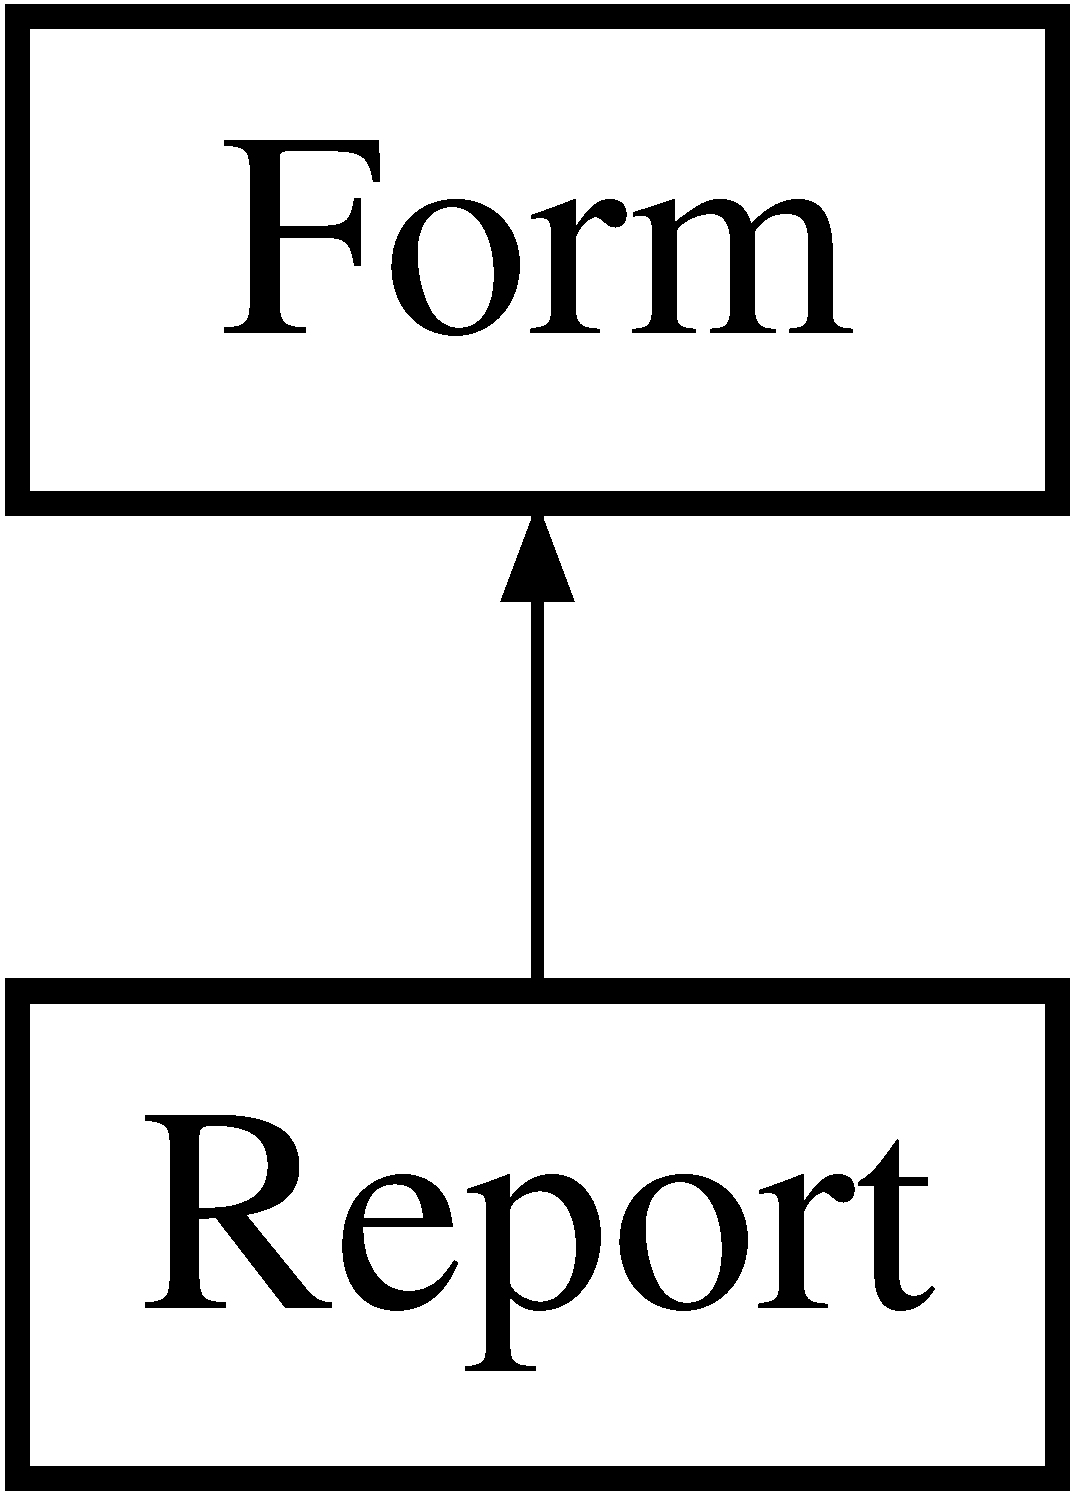
\includegraphics[height=2.000000cm]{classWildlifeTrackingApp_1_1Report}
\end{center}
\end{figure}
\subsection*{Public Member Functions}
\begin{DoxyCompactItemize}
\item 
\hyperlink{classWildlifeTrackingApp_1_1Report_a62bc0d20ce17d1ee1289cfccd4c0ce68}{Report} ()
\end{DoxyCompactItemize}
\subsection*{Public Attributes}
\begin{DoxyCompactItemize}
\item 
Date\+Time \hyperlink{classWildlifeTrackingApp_1_1Report_a3ee65fd5edda8ee4040edc92e50acfc5}{from\+Date} = Date\+Time.\+Now
\item 
Date\+Time \hyperlink{classWildlifeTrackingApp_1_1Report_a6c861174d14c06304507891ae7ee89cf}{to\+Date} = Date\+Time.\+Now
\end{DoxyCompactItemize}
\subsection*{Protected Member Functions}
\begin{DoxyCompactItemize}
\item 
override void \hyperlink{classWildlifeTrackingApp_1_1Report_a849c3c7f8d08104f0cdb46bee9fe6389}{Dispose} (bool disposing)
\begin{DoxyCompactList}\small\item\em Clean up any resources being used. \end{DoxyCompactList}\end{DoxyCompactItemize}
\subsection*{Properties}
\begin{DoxyCompactItemize}
\item 
static log4net.\+I\+Log \hyperlink{classWildlifeTrackingApp_1_1Report_a5fc9abb86e6110ecd61d0a1a7d740a8a}{Log}\hspace{0.3cm}{\ttfamily  \mbox{[}get, private set\mbox{]}}
\end{DoxyCompactItemize}
\subsection*{Private Member Functions}
\begin{DoxyCompactItemize}
\item 
void \hyperlink{classWildlifeTrackingApp_1_1Report_a0f200b495bdf3a236fb9c28c94b80c3e}{from\+Date\+Picker\+\_\+\+Value\+Changed} (object sender, Event\+Args e)
\begin{DoxyCompactList}\small\item\em Event handler for the change in the value of fromdate picker. \end{DoxyCompactList}\item 
void \hyperlink{classWildlifeTrackingApp_1_1Report_a7c96e63901fb6957f166378e24e989a6}{generate\+\_\+button\+\_\+\+Click} (object sender, Event\+Args e)
\begin{DoxyCompactList}\small\item\em Event handler for the generate button click. It generates charts based on total number of animals per category. \end{DoxyCompactList}\item 
void \hyperlink{classWildlifeTrackingApp_1_1Report_a6405d5db675d5338663195a4d12b4c9f}{Initialize\+Component} ()
\begin{DoxyCompactList}\small\item\em Required method for Designer support -\/ do not modify the contents of this method with the code editor. \end{DoxyCompactList}\item 
void \hyperlink{classWildlifeTrackingApp_1_1Report_a689e29ad27d8dabef272ce565669e8d9}{Report\+\_\+\+Load} (object sender, Event\+Args e)
\begin{DoxyCompactList}\small\item\em Event handler for form load. Customizes the datetime picker format. \end{DoxyCompactList}\item 
void \hyperlink{classWildlifeTrackingApp_1_1Report_a2a3664c6456b8f19a68866509ec3d802}{report\+Generation\+\_\+\+Activated} (object sender, Event\+Args e)
\begin{DoxyCompactList}\small\item\em Event handler for the activation of form. \end{DoxyCompactList}\item 
void \hyperlink{classWildlifeTrackingApp_1_1Report_a3479aaacdf8b5caeede09ea6a098e25f}{to\+Date\+Picker\+\_\+\+Value\+Changed} (object sender, Event\+Args e)
\begin{DoxyCompactList}\small\item\em Event handler for the change in the value of todate picker. \end{DoxyCompactList}\end{DoxyCompactItemize}
\subsection*{Private Attributes}
\begin{DoxyCompactItemize}
\item 
System.\+Component\+Model.\+I\+Container \hyperlink{classWildlifeTrackingApp_1_1Report_a02595f1c09713bb71dcb2fbbfc7ffa4b}{components} = null
\begin{DoxyCompactList}\small\item\em Required designer variable. \end{DoxyCompactList}\item 
System.\+Windows.\+Forms.\+Label \hyperlink{classWildlifeTrackingApp_1_1Report_ae086ffc402f846f057da52c2e5f5e9b5}{from\+Date\+\_\+label}
\item 
System.\+Windows.\+Forms.\+Date\+Time\+Picker \hyperlink{classWildlifeTrackingApp_1_1Report_abff71dccee21e2fcd7b2e912b3b7c608}{from\+Date\+Picker}
\item 
System.\+Windows.\+Forms.\+Button \hyperlink{classWildlifeTrackingApp_1_1Report_a44b2ab91fc54d54d9ef460e816ae272e}{generate\+\_\+button}
\item 
System.\+Windows.\+Forms.\+Data\+Visualization.\+Charting.\+Chart \hyperlink{classWildlifeTrackingApp_1_1Report_a9ba237d7da8d44242a02064a69dc9bcd}{report\+Chart}
\item 
System.\+Windows.\+Forms.\+Label \hyperlink{classWildlifeTrackingApp_1_1Report_a1534049397f4b7ab97324f502b5f5335}{to\+Date\+\_\+label}
\item 
System.\+Windows.\+Forms.\+Date\+Time\+Picker \hyperlink{classWildlifeTrackingApp_1_1Report_afd2fec8eb0f1c33b3b723a6d349c20ed}{to\+Date\+Picker}
\end{DoxyCompactItemize}
\subsection*{Static Private Attributes}
\begin{DoxyCompactItemize}
\item 
static readonly log4net.\+I\+Log \hyperlink{classWildlifeTrackingApp_1_1Report_ae6c6142b8525b2f4ac6ee6e003b3106f}{log}
\end{DoxyCompactItemize}


\subsection{Detailed Description}
Form class for the report generation page. Generates report of total number of animals per categories based on the from and to date. 



\subsection{Constructor \& Destructor Documentation}
\mbox{\Hypertarget{classWildlifeTrackingApp_1_1Report_a62bc0d20ce17d1ee1289cfccd4c0ce68}\label{classWildlifeTrackingApp_1_1Report_a62bc0d20ce17d1ee1289cfccd4c0ce68}} 
\index{Wildlife\+Tracking\+App\+::\+Report@{Wildlife\+Tracking\+App\+::\+Report}!Report@{Report}}
\index{Report@{Report}!Wildlife\+Tracking\+App\+::\+Report@{Wildlife\+Tracking\+App\+::\+Report}}
\subsubsection{\texorpdfstring{Report()}{Report()}}
{\footnotesize\ttfamily \hyperlink{classWildlifeTrackingApp_1_1Report}{Report} (\begin{DoxyParamCaption}{ }\end{DoxyParamCaption})\hspace{0.3cm}{\ttfamily [inline]}}



\subsection{Member Function Documentation}
\mbox{\Hypertarget{classWildlifeTrackingApp_1_1Report_a849c3c7f8d08104f0cdb46bee9fe6389}\label{classWildlifeTrackingApp_1_1Report_a849c3c7f8d08104f0cdb46bee9fe6389}} 
\index{Wildlife\+Tracking\+App\+::\+Report@{Wildlife\+Tracking\+App\+::\+Report}!Dispose@{Dispose}}
\index{Dispose@{Dispose}!Wildlife\+Tracking\+App\+::\+Report@{Wildlife\+Tracking\+App\+::\+Report}}
\subsubsection{\texorpdfstring{Dispose()}{Dispose()}}
{\footnotesize\ttfamily override void Dispose (\begin{DoxyParamCaption}\item[{bool}]{disposing }\end{DoxyParamCaption})\hspace{0.3cm}{\ttfamily [inline]}, {\ttfamily [protected]}}



Clean up any resources being used. 


\begin{DoxyParams}{Parameters}
{\em disposing} & true if managed resources should be disposed; otherwise, false.\\
\hline
\end{DoxyParams}
\mbox{\Hypertarget{classWildlifeTrackingApp_1_1Report_a0f200b495bdf3a236fb9c28c94b80c3e}\label{classWildlifeTrackingApp_1_1Report_a0f200b495bdf3a236fb9c28c94b80c3e}} 
\index{Wildlife\+Tracking\+App\+::\+Report@{Wildlife\+Tracking\+App\+::\+Report}!from\+Date\+Picker\+\_\+\+Value\+Changed@{from\+Date\+Picker\+\_\+\+Value\+Changed}}
\index{from\+Date\+Picker\+\_\+\+Value\+Changed@{from\+Date\+Picker\+\_\+\+Value\+Changed}!Wildlife\+Tracking\+App\+::\+Report@{Wildlife\+Tracking\+App\+::\+Report}}
\subsubsection{\texorpdfstring{from\+Date\+Picker\+\_\+\+Value\+Changed()}{fromDatePicker\_ValueChanged()}}
{\footnotesize\ttfamily void from\+Date\+Picker\+\_\+\+Value\+Changed (\begin{DoxyParamCaption}\item[{object}]{sender,  }\item[{Event\+Args}]{e }\end{DoxyParamCaption})\hspace{0.3cm}{\ttfamily [inline]}, {\ttfamily [private]}}



Event handler for the change in the value of fromdate picker. 


\begin{DoxyParams}{Parameters}
{\em sender} & Sender Object\\
\hline
{\em e} & Event argument\\
\hline
\end{DoxyParams}
\mbox{\Hypertarget{classWildlifeTrackingApp_1_1Report_a7c96e63901fb6957f166378e24e989a6}\label{classWildlifeTrackingApp_1_1Report_a7c96e63901fb6957f166378e24e989a6}} 
\index{Wildlife\+Tracking\+App\+::\+Report@{Wildlife\+Tracking\+App\+::\+Report}!generate\+\_\+button\+\_\+\+Click@{generate\+\_\+button\+\_\+\+Click}}
\index{generate\+\_\+button\+\_\+\+Click@{generate\+\_\+button\+\_\+\+Click}!Wildlife\+Tracking\+App\+::\+Report@{Wildlife\+Tracking\+App\+::\+Report}}
\subsubsection{\texorpdfstring{generate\+\_\+button\+\_\+\+Click()}{generate\_button\_Click()}}
{\footnotesize\ttfamily void generate\+\_\+button\+\_\+\+Click (\begin{DoxyParamCaption}\item[{object}]{sender,  }\item[{Event\+Args}]{e }\end{DoxyParamCaption})\hspace{0.3cm}{\ttfamily [inline]}, {\ttfamily [private]}}



Event handler for the generate button click. It generates charts based on total number of animals per category. 


\begin{DoxyParams}{Parameters}
{\em sender} & Sender Object\\
\hline
{\em e} & Event argument\\
\hline
\end{DoxyParams}
\mbox{\Hypertarget{classWildlifeTrackingApp_1_1Report_a6405d5db675d5338663195a4d12b4c9f}\label{classWildlifeTrackingApp_1_1Report_a6405d5db675d5338663195a4d12b4c9f}} 
\index{Wildlife\+Tracking\+App\+::\+Report@{Wildlife\+Tracking\+App\+::\+Report}!Initialize\+Component@{Initialize\+Component}}
\index{Initialize\+Component@{Initialize\+Component}!Wildlife\+Tracking\+App\+::\+Report@{Wildlife\+Tracking\+App\+::\+Report}}
\subsubsection{\texorpdfstring{Initialize\+Component()}{InitializeComponent()}}
{\footnotesize\ttfamily void Initialize\+Component (\begin{DoxyParamCaption}{ }\end{DoxyParamCaption})\hspace{0.3cm}{\ttfamily [inline]}, {\ttfamily [private]}}



Required method for Designer support -\/ do not modify the contents of this method with the code editor. 

\mbox{\Hypertarget{classWildlifeTrackingApp_1_1Report_a689e29ad27d8dabef272ce565669e8d9}\label{classWildlifeTrackingApp_1_1Report_a689e29ad27d8dabef272ce565669e8d9}} 
\index{Wildlife\+Tracking\+App\+::\+Report@{Wildlife\+Tracking\+App\+::\+Report}!Report\+\_\+\+Load@{Report\+\_\+\+Load}}
\index{Report\+\_\+\+Load@{Report\+\_\+\+Load}!Wildlife\+Tracking\+App\+::\+Report@{Wildlife\+Tracking\+App\+::\+Report}}
\subsubsection{\texorpdfstring{Report\+\_\+\+Load()}{Report\_Load()}}
{\footnotesize\ttfamily void Report\+\_\+\+Load (\begin{DoxyParamCaption}\item[{object}]{sender,  }\item[{Event\+Args}]{e }\end{DoxyParamCaption})\hspace{0.3cm}{\ttfamily [inline]}, {\ttfamily [private]}}



Event handler for form load. Customizes the datetime picker format. 


\begin{DoxyParams}{Parameters}
{\em sender} & \\
\hline
{\em e} & \\
\hline
\end{DoxyParams}
\mbox{\Hypertarget{classWildlifeTrackingApp_1_1Report_a2a3664c6456b8f19a68866509ec3d802}\label{classWildlifeTrackingApp_1_1Report_a2a3664c6456b8f19a68866509ec3d802}} 
\index{Wildlife\+Tracking\+App\+::\+Report@{Wildlife\+Tracking\+App\+::\+Report}!report\+Generation\+\_\+\+Activated@{report\+Generation\+\_\+\+Activated}}
\index{report\+Generation\+\_\+\+Activated@{report\+Generation\+\_\+\+Activated}!Wildlife\+Tracking\+App\+::\+Report@{Wildlife\+Tracking\+App\+::\+Report}}
\subsubsection{\texorpdfstring{report\+Generation\+\_\+\+Activated()}{reportGeneration\_Activated()}}
{\footnotesize\ttfamily void report\+Generation\+\_\+\+Activated (\begin{DoxyParamCaption}\item[{object}]{sender,  }\item[{Event\+Args}]{e }\end{DoxyParamCaption})\hspace{0.3cm}{\ttfamily [inline]}, {\ttfamily [private]}}



Event handler for the activation of form. 


\begin{DoxyParams}{Parameters}
{\em sender} & Sender Object\\
\hline
{\em e} & Event argument\\
\hline
\end{DoxyParams}
\mbox{\Hypertarget{classWildlifeTrackingApp_1_1Report_a3479aaacdf8b5caeede09ea6a098e25f}\label{classWildlifeTrackingApp_1_1Report_a3479aaacdf8b5caeede09ea6a098e25f}} 
\index{Wildlife\+Tracking\+App\+::\+Report@{Wildlife\+Tracking\+App\+::\+Report}!to\+Date\+Picker\+\_\+\+Value\+Changed@{to\+Date\+Picker\+\_\+\+Value\+Changed}}
\index{to\+Date\+Picker\+\_\+\+Value\+Changed@{to\+Date\+Picker\+\_\+\+Value\+Changed}!Wildlife\+Tracking\+App\+::\+Report@{Wildlife\+Tracking\+App\+::\+Report}}
\subsubsection{\texorpdfstring{to\+Date\+Picker\+\_\+\+Value\+Changed()}{toDatePicker\_ValueChanged()}}
{\footnotesize\ttfamily void to\+Date\+Picker\+\_\+\+Value\+Changed (\begin{DoxyParamCaption}\item[{object}]{sender,  }\item[{Event\+Args}]{e }\end{DoxyParamCaption})\hspace{0.3cm}{\ttfamily [inline]}, {\ttfamily [private]}}



Event handler for the change in the value of todate picker. 


\begin{DoxyParams}{Parameters}
{\em sender} & Sender Object\\
\hline
{\em e} & Event argument\\
\hline
\end{DoxyParams}


\subsection{Member Data Documentation}
\mbox{\Hypertarget{classWildlifeTrackingApp_1_1Report_a02595f1c09713bb71dcb2fbbfc7ffa4b}\label{classWildlifeTrackingApp_1_1Report_a02595f1c09713bb71dcb2fbbfc7ffa4b}} 
\index{Wildlife\+Tracking\+App\+::\+Report@{Wildlife\+Tracking\+App\+::\+Report}!components@{components}}
\index{components@{components}!Wildlife\+Tracking\+App\+::\+Report@{Wildlife\+Tracking\+App\+::\+Report}}
\subsubsection{\texorpdfstring{components}{components}}
{\footnotesize\ttfamily System.\+Component\+Model.\+I\+Container components = null\hspace{0.3cm}{\ttfamily [private]}}



Required designer variable. 

\mbox{\Hypertarget{classWildlifeTrackingApp_1_1Report_a3ee65fd5edda8ee4040edc92e50acfc5}\label{classWildlifeTrackingApp_1_1Report_a3ee65fd5edda8ee4040edc92e50acfc5}} 
\index{Wildlife\+Tracking\+App\+::\+Report@{Wildlife\+Tracking\+App\+::\+Report}!from\+Date@{from\+Date}}
\index{from\+Date@{from\+Date}!Wildlife\+Tracking\+App\+::\+Report@{Wildlife\+Tracking\+App\+::\+Report}}
\subsubsection{\texorpdfstring{from\+Date}{fromDate}}
{\footnotesize\ttfamily Date\+Time from\+Date = Date\+Time.\+Now}

\mbox{\Hypertarget{classWildlifeTrackingApp_1_1Report_ae086ffc402f846f057da52c2e5f5e9b5}\label{classWildlifeTrackingApp_1_1Report_ae086ffc402f846f057da52c2e5f5e9b5}} 
\index{Wildlife\+Tracking\+App\+::\+Report@{Wildlife\+Tracking\+App\+::\+Report}!from\+Date\+\_\+label@{from\+Date\+\_\+label}}
\index{from\+Date\+\_\+label@{from\+Date\+\_\+label}!Wildlife\+Tracking\+App\+::\+Report@{Wildlife\+Tracking\+App\+::\+Report}}
\subsubsection{\texorpdfstring{from\+Date\+\_\+label}{fromDate\_label}}
{\footnotesize\ttfamily System.\+Windows.\+Forms.\+Label from\+Date\+\_\+label\hspace{0.3cm}{\ttfamily [private]}}

\mbox{\Hypertarget{classWildlifeTrackingApp_1_1Report_abff71dccee21e2fcd7b2e912b3b7c608}\label{classWildlifeTrackingApp_1_1Report_abff71dccee21e2fcd7b2e912b3b7c608}} 
\index{Wildlife\+Tracking\+App\+::\+Report@{Wildlife\+Tracking\+App\+::\+Report}!from\+Date\+Picker@{from\+Date\+Picker}}
\index{from\+Date\+Picker@{from\+Date\+Picker}!Wildlife\+Tracking\+App\+::\+Report@{Wildlife\+Tracking\+App\+::\+Report}}
\subsubsection{\texorpdfstring{from\+Date\+Picker}{fromDatePicker}}
{\footnotesize\ttfamily System.\+Windows.\+Forms.\+Date\+Time\+Picker from\+Date\+Picker\hspace{0.3cm}{\ttfamily [private]}}

\mbox{\Hypertarget{classWildlifeTrackingApp_1_1Report_a44b2ab91fc54d54d9ef460e816ae272e}\label{classWildlifeTrackingApp_1_1Report_a44b2ab91fc54d54d9ef460e816ae272e}} 
\index{Wildlife\+Tracking\+App\+::\+Report@{Wildlife\+Tracking\+App\+::\+Report}!generate\+\_\+button@{generate\+\_\+button}}
\index{generate\+\_\+button@{generate\+\_\+button}!Wildlife\+Tracking\+App\+::\+Report@{Wildlife\+Tracking\+App\+::\+Report}}
\subsubsection{\texorpdfstring{generate\+\_\+button}{generate\_button}}
{\footnotesize\ttfamily System.\+Windows.\+Forms.\+Button generate\+\_\+button\hspace{0.3cm}{\ttfamily [private]}}

\mbox{\Hypertarget{classWildlifeTrackingApp_1_1Report_ae6c6142b8525b2f4ac6ee6e003b3106f}\label{classWildlifeTrackingApp_1_1Report_ae6c6142b8525b2f4ac6ee6e003b3106f}} 
\index{Wildlife\+Tracking\+App\+::\+Report@{Wildlife\+Tracking\+App\+::\+Report}!log@{log}}
\index{log@{log}!Wildlife\+Tracking\+App\+::\+Report@{Wildlife\+Tracking\+App\+::\+Report}}
\subsubsection{\texorpdfstring{log}{log}}
{\footnotesize\ttfamily readonly log4net.\+I\+Log log\hspace{0.3cm}{\ttfamily [static]}, {\ttfamily [private]}}

{\bfseries Initial value\+:}
\begin{DoxyCode}
= log4net.LogManager.GetLogger
        (\hyperlink{namespaceSystem}{System}.Reflection.MethodBase.GetCurrentMethod().DeclaringType)
\end{DoxyCode}
\mbox{\Hypertarget{classWildlifeTrackingApp_1_1Report_a9ba237d7da8d44242a02064a69dc9bcd}\label{classWildlifeTrackingApp_1_1Report_a9ba237d7da8d44242a02064a69dc9bcd}} 
\index{Wildlife\+Tracking\+App\+::\+Report@{Wildlife\+Tracking\+App\+::\+Report}!report\+Chart@{report\+Chart}}
\index{report\+Chart@{report\+Chart}!Wildlife\+Tracking\+App\+::\+Report@{Wildlife\+Tracking\+App\+::\+Report}}
\subsubsection{\texorpdfstring{report\+Chart}{reportChart}}
{\footnotesize\ttfamily System.\+Windows.\+Forms.\+Data\+Visualization.\+Charting.\+Chart report\+Chart\hspace{0.3cm}{\ttfamily [private]}}

\mbox{\Hypertarget{classWildlifeTrackingApp_1_1Report_a6c861174d14c06304507891ae7ee89cf}\label{classWildlifeTrackingApp_1_1Report_a6c861174d14c06304507891ae7ee89cf}} 
\index{Wildlife\+Tracking\+App\+::\+Report@{Wildlife\+Tracking\+App\+::\+Report}!to\+Date@{to\+Date}}
\index{to\+Date@{to\+Date}!Wildlife\+Tracking\+App\+::\+Report@{Wildlife\+Tracking\+App\+::\+Report}}
\subsubsection{\texorpdfstring{to\+Date}{toDate}}
{\footnotesize\ttfamily Date\+Time to\+Date = Date\+Time.\+Now}

\mbox{\Hypertarget{classWildlifeTrackingApp_1_1Report_a1534049397f4b7ab97324f502b5f5335}\label{classWildlifeTrackingApp_1_1Report_a1534049397f4b7ab97324f502b5f5335}} 
\index{Wildlife\+Tracking\+App\+::\+Report@{Wildlife\+Tracking\+App\+::\+Report}!to\+Date\+\_\+label@{to\+Date\+\_\+label}}
\index{to\+Date\+\_\+label@{to\+Date\+\_\+label}!Wildlife\+Tracking\+App\+::\+Report@{Wildlife\+Tracking\+App\+::\+Report}}
\subsubsection{\texorpdfstring{to\+Date\+\_\+label}{toDate\_label}}
{\footnotesize\ttfamily System.\+Windows.\+Forms.\+Label to\+Date\+\_\+label\hspace{0.3cm}{\ttfamily [private]}}

\mbox{\Hypertarget{classWildlifeTrackingApp_1_1Report_afd2fec8eb0f1c33b3b723a6d349c20ed}\label{classWildlifeTrackingApp_1_1Report_afd2fec8eb0f1c33b3b723a6d349c20ed}} 
\index{Wildlife\+Tracking\+App\+::\+Report@{Wildlife\+Tracking\+App\+::\+Report}!to\+Date\+Picker@{to\+Date\+Picker}}
\index{to\+Date\+Picker@{to\+Date\+Picker}!Wildlife\+Tracking\+App\+::\+Report@{Wildlife\+Tracking\+App\+::\+Report}}
\subsubsection{\texorpdfstring{to\+Date\+Picker}{toDatePicker}}
{\footnotesize\ttfamily System.\+Windows.\+Forms.\+Date\+Time\+Picker to\+Date\+Picker\hspace{0.3cm}{\ttfamily [private]}}



\subsection{Property Documentation}
\mbox{\Hypertarget{classWildlifeTrackingApp_1_1Report_a5fc9abb86e6110ecd61d0a1a7d740a8a}\label{classWildlifeTrackingApp_1_1Report_a5fc9abb86e6110ecd61d0a1a7d740a8a}} 
\index{Wildlife\+Tracking\+App\+::\+Report@{Wildlife\+Tracking\+App\+::\+Report}!Log@{Log}}
\index{Log@{Log}!Wildlife\+Tracking\+App\+::\+Report@{Wildlife\+Tracking\+App\+::\+Report}}
\subsubsection{\texorpdfstring{Log}{Log}}
{\footnotesize\ttfamily log4net.\+I\+Log Log\hspace{0.3cm}{\ttfamily [static]}, {\ttfamily [get]}, {\ttfamily [private set]}}



The documentation for this class was generated from the following files\+:\begin{DoxyCompactItemize}
\item 
View/\hyperlink{Report_8cs}{Report.\+cs}\item 
View/\hyperlink{Report_8Designer_8cs}{Report.\+Designer.\+cs}\end{DoxyCompactItemize}

\hypertarget{classWildlifeTrackingApp_1_1Utility_1_1Constants}{}\section{Constants}
\label{classWildlifeTrackingApp_1_1Utility_1_1Constants}\index{Constants@{Constants}}
\subsection*{Static Public Attributes}
\begin{DoxyCompactItemize}
\item 
static string \hyperlink{classWildlifeTrackingApp_1_1Utility_1_1Constants_a123c1c5bb235a2e006300c385c8af3c4}{A\+D\+D\+\_\+\+N\+E\+W\+\_\+\+A\+N\+I\+M\+A\+L\+\_\+\+U\+RL} = \char`\"{}Services/Animal\+Service.\+svc/v1/Add\+Animal\char`\"{}
\item 
static string \hyperlink{classWildlifeTrackingApp_1_1Utility_1_1Constants_adee90abc1a8828f9962b7a2f05b3fce6}{A\+D\+D\+\_\+\+N\+E\+W\+\_\+\+C\+A\+T\+E\+G\+O\+R\+Y\+\_\+\+U\+RL} = \char`\"{}Services/Category\+Service.\+svc/v1/add\+New\+Category\char`\"{}
\item 
static string \hyperlink{classWildlifeTrackingApp_1_1Utility_1_1Constants_a50a6829a782e9be781fa98bfa5a7f04e}{A\+LL} = \char`\"{}All\char`\"{}
\item 
static string \hyperlink{classWildlifeTrackingApp_1_1Utility_1_1Constants_a8e7cd9f72334c5cc9097557a2b873d7b}{C\+A\+T\+E\+G\+O\+R\+Y\+\_\+\+ID} = \char`\"{}category\+Id\char`\"{}
\item 
static string \hyperlink{classWildlifeTrackingApp_1_1Utility_1_1Constants_aa83ef34c140142171da77a3cec88cf7e}{C\+A\+T\+E\+G\+O\+R\+Y\+\_\+\+N\+A\+ME} = \char`\"{}Category\+Name\char`\"{}
\item 
static string \mbox{[}$\,$\mbox{]} \hyperlink{classWildlifeTrackingApp_1_1Utility_1_1Constants_a5f8721853059da36c3a719d8f04eb551}{Category\+Map\+Locator\+Color}
\item 
static string \hyperlink{classWildlifeTrackingApp_1_1Utility_1_1Constants_a9ffe83f09b9dd422b8b1f94a4f4a6a21}{C\+O\+L\+O\+N\+\_\+\+C\+O\+N\+S\+T\+A\+N\+TS} = \char`\"{}\+:\char`\"{}
\item 
static string \hyperlink{classWildlifeTrackingApp_1_1Utility_1_1Constants_ac70159f34c1d5ab4a729d8b789813775}{C\+O\+U\+NT} = \char`\"{}Count\char`\"{}
\item 
static string \hyperlink{classWildlifeTrackingApp_1_1Utility_1_1Constants_ae3ae8c5c26c8d602f72f2c040ecc038d}{C\+O\+U\+N\+T\+\_\+\+O\+F\+\_\+\+A\+L\+L\+\_\+\+T\+H\+E\+\_\+\+A\+N\+I\+M\+A\+L\+S\+\_\+\+P\+E\+R\+\_\+\+C\+A\+T\+E\+G\+O\+RY} = \char`\"{}C\+O\+U\+NT OF \hyperlink{classWildlifeTrackingApp_1_1Utility_1_1Constants_a50a6829a782e9be781fa98bfa5a7f04e}{A\+LL} T\+HE A\+N\+I\+M\+A\+LS P\+ER C\+A\+T\+E\+G\+O\+RY\char`\"{}
\item 
static string \hyperlink{classWildlifeTrackingApp_1_1Utility_1_1Constants_ad30b3b723d160b203f8ee9a4d2894368}{D\+A\+T\+E\+\_\+\+P\+I\+C\+K\+E\+R\+\_\+\+F\+O\+M\+AT} = \char`\"{}yyyy-\/MM-\/dd\char`\"{}
\item 
static string \hyperlink{classWildlifeTrackingApp_1_1Utility_1_1Constants_a79f17386a483eb46ced47455c8b2114e}{D\+E\+L\+E\+T\+E\+\_\+\+A\+N\+I\+M\+A\+L\+\_\+\+U\+RL} = \char`\"{}Services/Animal\+Service.\+svc/v1/delete\+Animal/\char`\"{}
\item 
static string \hyperlink{classWildlifeTrackingApp_1_1Utility_1_1Constants_a5bada733b70103a3673dca0d63bc0f79}{D\+E\+L\+E\+T\+E\+\_\+\+N\+E\+W\+\_\+\+C\+A\+T\+E\+G\+O\+R\+Y\+\_\+\+U\+RL} = \char`\"{}Services/Category\+Service.\+svc/v1/delete\+Category/\char`\"{}
\item 
static string \hyperlink{classWildlifeTrackingApp_1_1Utility_1_1Constants_afc4cd87d4d5553a12fc5a7b7e7b9a081}{E\+R\+R\+O\+R\+\_\+\+A\+N\+I\+M\+A\+L\+\_\+\+D\+E\+L\+E\+T\+I\+N\+G\+\_\+\+M\+E\+S\+S\+A\+GE} = \char`\"{}Error in delete animal\char`\"{}
\item 
static string \hyperlink{classWildlifeTrackingApp_1_1Utility_1_1Constants_a23507886683a294679c1916b50b7b2eb}{E\+R\+R\+O\+R\+\_\+\+C\+R\+E\+A\+T\+I\+N\+G\+\_\+\+C\+A\+T\+E\+G\+O\+R\+Y\+\_\+\+M\+E\+S\+S\+A\+GE} = \char`\"{}Error in deleting the \hyperlink{classWildlifeTrackingApp_1_1Category}{Category}\char`\"{}
\item 
static string \hyperlink{classWildlifeTrackingApp_1_1Utility_1_1Constants_a3677f3f16659ea015b9737c0b366dbe3}{E\+R\+R\+O\+R\+\_\+\+D\+E\+L\+E\+T\+I\+N\+G\+\_\+\+C\+A\+T\+E\+G\+O\+R\+Y\+\_\+\+M\+E\+S\+S\+A\+GE} = \char`\"{}Error in deleting the category\char`\"{}
\item 
static string \hyperlink{classWildlifeTrackingApp_1_1Utility_1_1Constants_a207801de28af5d299304a40cfb45a273}{E\+R\+R\+O\+R\+\_\+\+G\+P\+S\+\_\+\+A\+L\+L\+O\+C\+A\+T\+I\+O\+N\+\_\+\+M\+E\+S\+S\+A\+GE} = \char`\"{}Error in allocating the animal with G\+PS Device\char`\"{}
\item 
static string \hyperlink{classWildlifeTrackingApp_1_1Utility_1_1Constants_a688156a62d9b70ee7ddf29c359e50c4f}{F\+R\+O\+M\+\_\+\+D\+A\+T\+E\+\_\+\+V\+A\+L\+I\+D\+A\+T\+I\+O\+N\+\_\+\+M\+E\+S\+S\+A\+GE} = \char`\"{}From date should be less than present date/end date\char`\"{}
\item 
static string \hyperlink{classWildlifeTrackingApp_1_1Utility_1_1Constants_a5b11de05186392a645b8b03e863a0f0e}{G\+E\+T\+\_\+\+A\+L\+L\+\_\+\+A\+N\+I\+M\+A\+L\+S\+\_\+\+L\+A\+T\+E\+S\+T\+\_\+\+P\+O\+S\+I\+T\+I\+O\+N\+\_\+\+U\+RL} = \char`\"{}Services/Tracking\+Info\+Service.\+svc/v1/get\+All\+Animals\+Latest\+Location\char`\"{}
\item 
static string \hyperlink{classWildlifeTrackingApp_1_1Utility_1_1Constants_a57e74b3240cd0851eabf612486d7f9e3}{G\+E\+T\+\_\+\+A\+N\+I\+M\+A\+L\+\_\+\+C\+O\+U\+N\+T\+\_\+\+P\+E\+R\+\_\+\+C\+A\+T\+E\+G\+O\+R\+Y\+\_\+\+U\+RL} = \char`\"{}Services/Animal\+Service.\+svc/v1/get\+Animals\+Count\+Per\+Category/\char`\"{}
\item 
static string \hyperlink{classWildlifeTrackingApp_1_1Utility_1_1Constants_a4f1233471c34da67abf4bf0404a4f496}{G\+E\+T\+\_\+\+A\+N\+I\+M\+A\+L\+S\+\_\+\+L\+A\+T\+E\+S\+T\+\_\+\+P\+O\+S\+I\+T\+I\+O\+N\+\_\+\+P\+E\+R\+\_\+\+C\+A\+T\+E\+G\+O\+R\+Y\+\_\+\+U\+RL} = \char`\"{}Services/Tracking\+Info\+Service.\+svc/v1/get\+Each\+Category\+Animals\+Latest\+Location/\char`\"{}
\item 
static string \hyperlink{classWildlifeTrackingApp_1_1Utility_1_1Constants_a784acb2579317d1e18bd4d1ab4c81461}{G\+R\+E\+E\+N\+\_\+\+C\+O\+L\+OR} = \char`\"{}green\char`\"{}
\item 
static string \hyperlink{classWildlifeTrackingApp_1_1Utility_1_1Constants_a68104863796be82394071d37ec376133}{H\+A\+S\+H\+\_\+\+C\+O\+N\+S\+T\+A\+NT} = \char`\"{}\#\char`\"{}
\item 
static string \hyperlink{classWildlifeTrackingApp_1_1Utility_1_1Constants_afdc7b6bb94c9377a9e60acda8105859b}{L\+O\+C\+A\+T\+E\+\_\+\+A\+N\+I\+M\+A\+L\+\_\+\+H\+E\+A\+D\+I\+N\+G\+\_\+\+E\+N\+D\+\_\+\+A\+L\+L\+\_\+\+C\+A\+T\+E\+G\+O\+RY} = \char`\"{} categories\char`\"{}
\item 
static string \hyperlink{classWildlifeTrackingApp_1_1Utility_1_1Constants_a3f930b0b0329e9a6d8f433cbdff3a36d}{L\+O\+C\+A\+T\+E\+\_\+\+A\+N\+I\+M\+A\+L\+\_\+\+H\+E\+A\+D\+I\+N\+G\+\_\+\+E\+N\+D\+\_\+\+P\+E\+R\+\_\+\+C\+A\+T\+E\+G\+O\+RY} = \char`\"{} category\char`\"{}
\item 
static string \hyperlink{classWildlifeTrackingApp_1_1Utility_1_1Constants_a1935c9ba5401447e9f2c09ea6f36f3f5}{L\+O\+C\+A\+T\+E\+\_\+\+A\+N\+I\+M\+A\+L\+\_\+\+H\+E\+A\+D\+I\+N\+G\+\_\+\+S\+T\+A\+RT} = \char`\"{}Locating the animals of \char`\"{}
\item 
static string \hyperlink{classWildlifeTrackingApp_1_1Utility_1_1Constants_ab77321730fc5eb654915efb17d410aa7}{M\+A\+N\+D\+A\+T\+O\+R\+Y\+\_\+\+F\+I\+E\+L\+D\+\_\+\+E\+R\+R\+O\+R\+\_\+\+M\+E\+S\+S\+A\+GE} = \char`\"{}Mandatory fields need not be empty\char`\"{}
\item 
static string \hyperlink{classWildlifeTrackingApp_1_1Utility_1_1Constants_a2d7a4d0bda458906e6bca3a1ab24248c}{R\+E\+T\+R\+I\+E\+V\+E\+\_\+\+A\+L\+L\+\_\+\+A\+N\+I\+M\+A\+L\+\_\+\+U\+RL} = \char`\"{}Services/Animal\+Service.\+svc/v1/get\+All\+Animals\char`\"{}
\item 
static string \hyperlink{classWildlifeTrackingApp_1_1Utility_1_1Constants_a66a0208e68737d6c803afc8df55a04d1}{R\+E\+T\+R\+I\+E\+V\+E\+\_\+\+A\+L\+L\+\_\+\+C\+A\+T\+E\+G\+O\+R\+Y\+\_\+\+U\+RL} = \char`\"{}Services/Category\+Service.\+svc/v1/get\+Categories\char`\"{}
\item 
static string \hyperlink{classWildlifeTrackingApp_1_1Utility_1_1Constants_ab435d8d93e93bfe37f9969527966dfdf}{S\+U\+C\+C\+E\+S\+S\+F\+U\+L\+\_\+\+A\+D\+D\+\_\+\+C\+A\+T\+E\+G\+O\+R\+Y\+\_\+\+M\+E\+S\+S\+A\+GE} = \char`\"{}Successfully Added the \hyperlink{classWildlifeTrackingApp_1_1Category}{Category}\char`\"{}
\item 
static string \hyperlink{classWildlifeTrackingApp_1_1Utility_1_1Constants_a60b55ccb1b71163e8e94149114b40a3e}{S\+U\+C\+C\+E\+S\+S\+F\+U\+L\+\_\+\+A\+N\+I\+M\+A\+L\+\_\+\+D\+E\+L\+E\+T\+I\+N\+G\+\_\+\+M\+E\+S\+S\+A\+GE} = \char`\"{}Animal is deleted successfully\char`\"{}
\item 
static string \hyperlink{classWildlifeTrackingApp_1_1Utility_1_1Constants_a47b27471a06336a2eb79d2cd9dece230}{S\+U\+C\+C\+E\+S\+S\+F\+U\+L\+\_\+\+D\+E\+L\+E\+T\+E\+\_\+\+C\+A\+T\+E\+G\+O\+R\+Y\+\_\+\+M\+E\+S\+S\+A\+GE} = \char`\"{}Successfully deleted the \hyperlink{classWildlifeTrackingApp_1_1Category}{Category}\char`\"{}
\item 
static string \hyperlink{classWildlifeTrackingApp_1_1Utility_1_1Constants_ab7dec433f3af54f597bd520a55f39c9f}{S\+U\+C\+C\+E\+S\+S\+F\+U\+L\+L\+\_\+\+G\+P\+S\+\_\+\+A\+L\+L\+O\+C\+A\+T\+I\+O\+N\+\_\+\+M\+E\+S\+S\+A\+GE} = \char`\"{}Successfully added the animal and allocated with the G\+PS Device\char`\"{}
\item 
static string \hyperlink{classWildlifeTrackingApp_1_1Utility_1_1Constants_abaac5dc652e04ef9c20a970c7bcc5e59}{T\+O\+\_\+\+D\+A\+T\+E\+\_\+\+V\+A\+L\+I\+D\+A\+T\+I\+O\+N\+\_\+\+M\+E\+S\+S\+A\+GE} = \char`\"{}End date cannot be greater than present date\char`\"{}
\item 
static string \hyperlink{classWildlifeTrackingApp_1_1Utility_1_1Constants_acb342f6eb50039d8e87a136774d2bb43}{X86\+\_\+\+C\+O\+N\+S\+T\+A\+NT} = \char`\"{}X6\char`\"{}
\end{DoxyCompactItemize}


\subsection{Member Data Documentation}
\mbox{\Hypertarget{classWildlifeTrackingApp_1_1Utility_1_1Constants_a123c1c5bb235a2e006300c385c8af3c4}\label{classWildlifeTrackingApp_1_1Utility_1_1Constants_a123c1c5bb235a2e006300c385c8af3c4}} 
\index{Wildlife\+Tracking\+App\+::\+Utility\+::\+Constants@{Wildlife\+Tracking\+App\+::\+Utility\+::\+Constants}!A\+D\+D\+\_\+\+N\+E\+W\+\_\+\+A\+N\+I\+M\+A\+L\+\_\+\+U\+RL@{A\+D\+D\+\_\+\+N\+E\+W\+\_\+\+A\+N\+I\+M\+A\+L\+\_\+\+U\+RL}}
\index{A\+D\+D\+\_\+\+N\+E\+W\+\_\+\+A\+N\+I\+M\+A\+L\+\_\+\+U\+RL@{A\+D\+D\+\_\+\+N\+E\+W\+\_\+\+A\+N\+I\+M\+A\+L\+\_\+\+U\+RL}!Wildlife\+Tracking\+App\+::\+Utility\+::\+Constants@{Wildlife\+Tracking\+App\+::\+Utility\+::\+Constants}}
\subsubsection{\texorpdfstring{A\+D\+D\+\_\+\+N\+E\+W\+\_\+\+A\+N\+I\+M\+A\+L\+\_\+\+U\+RL}{ADD\_NEW\_ANIMAL\_URL}}
{\footnotesize\ttfamily string A\+D\+D\+\_\+\+N\+E\+W\+\_\+\+A\+N\+I\+M\+A\+L\+\_\+\+U\+RL = \char`\"{}Services/Animal\+Service.\+svc/v1/Add\+Animal\char`\"{}\hspace{0.3cm}{\ttfamily [static]}}

\mbox{\Hypertarget{classWildlifeTrackingApp_1_1Utility_1_1Constants_adee90abc1a8828f9962b7a2f05b3fce6}\label{classWildlifeTrackingApp_1_1Utility_1_1Constants_adee90abc1a8828f9962b7a2f05b3fce6}} 
\index{Wildlife\+Tracking\+App\+::\+Utility\+::\+Constants@{Wildlife\+Tracking\+App\+::\+Utility\+::\+Constants}!A\+D\+D\+\_\+\+N\+E\+W\+\_\+\+C\+A\+T\+E\+G\+O\+R\+Y\+\_\+\+U\+RL@{A\+D\+D\+\_\+\+N\+E\+W\+\_\+\+C\+A\+T\+E\+G\+O\+R\+Y\+\_\+\+U\+RL}}
\index{A\+D\+D\+\_\+\+N\+E\+W\+\_\+\+C\+A\+T\+E\+G\+O\+R\+Y\+\_\+\+U\+RL@{A\+D\+D\+\_\+\+N\+E\+W\+\_\+\+C\+A\+T\+E\+G\+O\+R\+Y\+\_\+\+U\+RL}!Wildlife\+Tracking\+App\+::\+Utility\+::\+Constants@{Wildlife\+Tracking\+App\+::\+Utility\+::\+Constants}}
\subsubsection{\texorpdfstring{A\+D\+D\+\_\+\+N\+E\+W\+\_\+\+C\+A\+T\+E\+G\+O\+R\+Y\+\_\+\+U\+RL}{ADD\_NEW\_CATEGORY\_URL}}
{\footnotesize\ttfamily string A\+D\+D\+\_\+\+N\+E\+W\+\_\+\+C\+A\+T\+E\+G\+O\+R\+Y\+\_\+\+U\+RL = \char`\"{}Services/Category\+Service.\+svc/v1/add\+New\+Category\char`\"{}\hspace{0.3cm}{\ttfamily [static]}}

\mbox{\Hypertarget{classWildlifeTrackingApp_1_1Utility_1_1Constants_a50a6829a782e9be781fa98bfa5a7f04e}\label{classWildlifeTrackingApp_1_1Utility_1_1Constants_a50a6829a782e9be781fa98bfa5a7f04e}} 
\index{Wildlife\+Tracking\+App\+::\+Utility\+::\+Constants@{Wildlife\+Tracking\+App\+::\+Utility\+::\+Constants}!A\+LL@{A\+LL}}
\index{A\+LL@{A\+LL}!Wildlife\+Tracking\+App\+::\+Utility\+::\+Constants@{Wildlife\+Tracking\+App\+::\+Utility\+::\+Constants}}
\subsubsection{\texorpdfstring{A\+LL}{ALL}}
{\footnotesize\ttfamily string A\+LL = \char`\"{}All\char`\"{}\hspace{0.3cm}{\ttfamily [static]}}

\mbox{\Hypertarget{classWildlifeTrackingApp_1_1Utility_1_1Constants_a8e7cd9f72334c5cc9097557a2b873d7b}\label{classWildlifeTrackingApp_1_1Utility_1_1Constants_a8e7cd9f72334c5cc9097557a2b873d7b}} 
\index{Wildlife\+Tracking\+App\+::\+Utility\+::\+Constants@{Wildlife\+Tracking\+App\+::\+Utility\+::\+Constants}!C\+A\+T\+E\+G\+O\+R\+Y\+\_\+\+ID@{C\+A\+T\+E\+G\+O\+R\+Y\+\_\+\+ID}}
\index{C\+A\+T\+E\+G\+O\+R\+Y\+\_\+\+ID@{C\+A\+T\+E\+G\+O\+R\+Y\+\_\+\+ID}!Wildlife\+Tracking\+App\+::\+Utility\+::\+Constants@{Wildlife\+Tracking\+App\+::\+Utility\+::\+Constants}}
\subsubsection{\texorpdfstring{C\+A\+T\+E\+G\+O\+R\+Y\+\_\+\+ID}{CATEGORY\_ID}}
{\footnotesize\ttfamily string C\+A\+T\+E\+G\+O\+R\+Y\+\_\+\+ID = \char`\"{}category\+Id\char`\"{}\hspace{0.3cm}{\ttfamily [static]}}

\mbox{\Hypertarget{classWildlifeTrackingApp_1_1Utility_1_1Constants_aa83ef34c140142171da77a3cec88cf7e}\label{classWildlifeTrackingApp_1_1Utility_1_1Constants_aa83ef34c140142171da77a3cec88cf7e}} 
\index{Wildlife\+Tracking\+App\+::\+Utility\+::\+Constants@{Wildlife\+Tracking\+App\+::\+Utility\+::\+Constants}!C\+A\+T\+E\+G\+O\+R\+Y\+\_\+\+N\+A\+ME@{C\+A\+T\+E\+G\+O\+R\+Y\+\_\+\+N\+A\+ME}}
\index{C\+A\+T\+E\+G\+O\+R\+Y\+\_\+\+N\+A\+ME@{C\+A\+T\+E\+G\+O\+R\+Y\+\_\+\+N\+A\+ME}!Wildlife\+Tracking\+App\+::\+Utility\+::\+Constants@{Wildlife\+Tracking\+App\+::\+Utility\+::\+Constants}}
\subsubsection{\texorpdfstring{C\+A\+T\+E\+G\+O\+R\+Y\+\_\+\+N\+A\+ME}{CATEGORY\_NAME}}
{\footnotesize\ttfamily string C\+A\+T\+E\+G\+O\+R\+Y\+\_\+\+N\+A\+ME = \char`\"{}Category\+Name\char`\"{}\hspace{0.3cm}{\ttfamily [static]}}

\mbox{\Hypertarget{classWildlifeTrackingApp_1_1Utility_1_1Constants_a5f8721853059da36c3a719d8f04eb551}\label{classWildlifeTrackingApp_1_1Utility_1_1Constants_a5f8721853059da36c3a719d8f04eb551}} 
\index{Wildlife\+Tracking\+App\+::\+Utility\+::\+Constants@{Wildlife\+Tracking\+App\+::\+Utility\+::\+Constants}!Category\+Map\+Locator\+Color@{Category\+Map\+Locator\+Color}}
\index{Category\+Map\+Locator\+Color@{Category\+Map\+Locator\+Color}!Wildlife\+Tracking\+App\+::\+Utility\+::\+Constants@{Wildlife\+Tracking\+App\+::\+Utility\+::\+Constants}}
\subsubsection{\texorpdfstring{Category\+Map\+Locator\+Color}{CategoryMapLocatorColor}}
{\footnotesize\ttfamily string \mbox{[}$\,$\mbox{]} Category\+Map\+Locator\+Color\hspace{0.3cm}{\ttfamily [static]}}

\mbox{\Hypertarget{classWildlifeTrackingApp_1_1Utility_1_1Constants_a9ffe83f09b9dd422b8b1f94a4f4a6a21}\label{classWildlifeTrackingApp_1_1Utility_1_1Constants_a9ffe83f09b9dd422b8b1f94a4f4a6a21}} 
\index{Wildlife\+Tracking\+App\+::\+Utility\+::\+Constants@{Wildlife\+Tracking\+App\+::\+Utility\+::\+Constants}!C\+O\+L\+O\+N\+\_\+\+C\+O\+N\+S\+T\+A\+N\+TS@{C\+O\+L\+O\+N\+\_\+\+C\+O\+N\+S\+T\+A\+N\+TS}}
\index{C\+O\+L\+O\+N\+\_\+\+C\+O\+N\+S\+T\+A\+N\+TS@{C\+O\+L\+O\+N\+\_\+\+C\+O\+N\+S\+T\+A\+N\+TS}!Wildlife\+Tracking\+App\+::\+Utility\+::\+Constants@{Wildlife\+Tracking\+App\+::\+Utility\+::\+Constants}}
\subsubsection{\texorpdfstring{C\+O\+L\+O\+N\+\_\+\+C\+O\+N\+S\+T\+A\+N\+TS}{COLON\_CONSTANTS}}
{\footnotesize\ttfamily string C\+O\+L\+O\+N\+\_\+\+C\+O\+N\+S\+T\+A\+N\+TS = \char`\"{}\+:\char`\"{}\hspace{0.3cm}{\ttfamily [static]}}

\mbox{\Hypertarget{classWildlifeTrackingApp_1_1Utility_1_1Constants_ac70159f34c1d5ab4a729d8b789813775}\label{classWildlifeTrackingApp_1_1Utility_1_1Constants_ac70159f34c1d5ab4a729d8b789813775}} 
\index{Wildlife\+Tracking\+App\+::\+Utility\+::\+Constants@{Wildlife\+Tracking\+App\+::\+Utility\+::\+Constants}!C\+O\+U\+NT@{C\+O\+U\+NT}}
\index{C\+O\+U\+NT@{C\+O\+U\+NT}!Wildlife\+Tracking\+App\+::\+Utility\+::\+Constants@{Wildlife\+Tracking\+App\+::\+Utility\+::\+Constants}}
\subsubsection{\texorpdfstring{C\+O\+U\+NT}{COUNT}}
{\footnotesize\ttfamily string C\+O\+U\+NT = \char`\"{}Count\char`\"{}\hspace{0.3cm}{\ttfamily [static]}}

\mbox{\Hypertarget{classWildlifeTrackingApp_1_1Utility_1_1Constants_ae3ae8c5c26c8d602f72f2c040ecc038d}\label{classWildlifeTrackingApp_1_1Utility_1_1Constants_ae3ae8c5c26c8d602f72f2c040ecc038d}} 
\index{Wildlife\+Tracking\+App\+::\+Utility\+::\+Constants@{Wildlife\+Tracking\+App\+::\+Utility\+::\+Constants}!C\+O\+U\+N\+T\+\_\+\+O\+F\+\_\+\+A\+L\+L\+\_\+\+T\+H\+E\+\_\+\+A\+N\+I\+M\+A\+L\+S\+\_\+\+P\+E\+R\+\_\+\+C\+A\+T\+E\+G\+O\+RY@{C\+O\+U\+N\+T\+\_\+\+O\+F\+\_\+\+A\+L\+L\+\_\+\+T\+H\+E\+\_\+\+A\+N\+I\+M\+A\+L\+S\+\_\+\+P\+E\+R\+\_\+\+C\+A\+T\+E\+G\+O\+RY}}
\index{C\+O\+U\+N\+T\+\_\+\+O\+F\+\_\+\+A\+L\+L\+\_\+\+T\+H\+E\+\_\+\+A\+N\+I\+M\+A\+L\+S\+\_\+\+P\+E\+R\+\_\+\+C\+A\+T\+E\+G\+O\+RY@{C\+O\+U\+N\+T\+\_\+\+O\+F\+\_\+\+A\+L\+L\+\_\+\+T\+H\+E\+\_\+\+A\+N\+I\+M\+A\+L\+S\+\_\+\+P\+E\+R\+\_\+\+C\+A\+T\+E\+G\+O\+RY}!Wildlife\+Tracking\+App\+::\+Utility\+::\+Constants@{Wildlife\+Tracking\+App\+::\+Utility\+::\+Constants}}
\subsubsection{\texorpdfstring{C\+O\+U\+N\+T\+\_\+\+O\+F\+\_\+\+A\+L\+L\+\_\+\+T\+H\+E\+\_\+\+A\+N\+I\+M\+A\+L\+S\+\_\+\+P\+E\+R\+\_\+\+C\+A\+T\+E\+G\+O\+RY}{COUNT\_OF\_ALL\_THE\_ANIMALS\_PER\_CATEGORY}}
{\footnotesize\ttfamily string C\+O\+U\+N\+T\+\_\+\+O\+F\+\_\+\+A\+L\+L\+\_\+\+T\+H\+E\+\_\+\+A\+N\+I\+M\+A\+L\+S\+\_\+\+P\+E\+R\+\_\+\+C\+A\+T\+E\+G\+O\+RY = \char`\"{}C\+O\+U\+NT OF \hyperlink{classWildlifeTrackingApp_1_1Utility_1_1Constants_a50a6829a782e9be781fa98bfa5a7f04e}{A\+LL} T\+HE A\+N\+I\+M\+A\+LS P\+ER C\+A\+T\+E\+G\+O\+RY\char`\"{}\hspace{0.3cm}{\ttfamily [static]}}

\mbox{\Hypertarget{classWildlifeTrackingApp_1_1Utility_1_1Constants_ad30b3b723d160b203f8ee9a4d2894368}\label{classWildlifeTrackingApp_1_1Utility_1_1Constants_ad30b3b723d160b203f8ee9a4d2894368}} 
\index{Wildlife\+Tracking\+App\+::\+Utility\+::\+Constants@{Wildlife\+Tracking\+App\+::\+Utility\+::\+Constants}!D\+A\+T\+E\+\_\+\+P\+I\+C\+K\+E\+R\+\_\+\+F\+O\+M\+AT@{D\+A\+T\+E\+\_\+\+P\+I\+C\+K\+E\+R\+\_\+\+F\+O\+M\+AT}}
\index{D\+A\+T\+E\+\_\+\+P\+I\+C\+K\+E\+R\+\_\+\+F\+O\+M\+AT@{D\+A\+T\+E\+\_\+\+P\+I\+C\+K\+E\+R\+\_\+\+F\+O\+M\+AT}!Wildlife\+Tracking\+App\+::\+Utility\+::\+Constants@{Wildlife\+Tracking\+App\+::\+Utility\+::\+Constants}}
\subsubsection{\texorpdfstring{D\+A\+T\+E\+\_\+\+P\+I\+C\+K\+E\+R\+\_\+\+F\+O\+M\+AT}{DATE\_PICKER\_FOMAT}}
{\footnotesize\ttfamily string D\+A\+T\+E\+\_\+\+P\+I\+C\+K\+E\+R\+\_\+\+F\+O\+M\+AT = \char`\"{}yyyy-\/MM-\/dd\char`\"{}\hspace{0.3cm}{\ttfamily [static]}}

\mbox{\Hypertarget{classWildlifeTrackingApp_1_1Utility_1_1Constants_a79f17386a483eb46ced47455c8b2114e}\label{classWildlifeTrackingApp_1_1Utility_1_1Constants_a79f17386a483eb46ced47455c8b2114e}} 
\index{Wildlife\+Tracking\+App\+::\+Utility\+::\+Constants@{Wildlife\+Tracking\+App\+::\+Utility\+::\+Constants}!D\+E\+L\+E\+T\+E\+\_\+\+A\+N\+I\+M\+A\+L\+\_\+\+U\+RL@{D\+E\+L\+E\+T\+E\+\_\+\+A\+N\+I\+M\+A\+L\+\_\+\+U\+RL}}
\index{D\+E\+L\+E\+T\+E\+\_\+\+A\+N\+I\+M\+A\+L\+\_\+\+U\+RL@{D\+E\+L\+E\+T\+E\+\_\+\+A\+N\+I\+M\+A\+L\+\_\+\+U\+RL}!Wildlife\+Tracking\+App\+::\+Utility\+::\+Constants@{Wildlife\+Tracking\+App\+::\+Utility\+::\+Constants}}
\subsubsection{\texorpdfstring{D\+E\+L\+E\+T\+E\+\_\+\+A\+N\+I\+M\+A\+L\+\_\+\+U\+RL}{DELETE\_ANIMAL\_URL}}
{\footnotesize\ttfamily string D\+E\+L\+E\+T\+E\+\_\+\+A\+N\+I\+M\+A\+L\+\_\+\+U\+RL = \char`\"{}Services/Animal\+Service.\+svc/v1/delete\+Animal/\char`\"{}\hspace{0.3cm}{\ttfamily [static]}}

\mbox{\Hypertarget{classWildlifeTrackingApp_1_1Utility_1_1Constants_a5bada733b70103a3673dca0d63bc0f79}\label{classWildlifeTrackingApp_1_1Utility_1_1Constants_a5bada733b70103a3673dca0d63bc0f79}} 
\index{Wildlife\+Tracking\+App\+::\+Utility\+::\+Constants@{Wildlife\+Tracking\+App\+::\+Utility\+::\+Constants}!D\+E\+L\+E\+T\+E\+\_\+\+N\+E\+W\+\_\+\+C\+A\+T\+E\+G\+O\+R\+Y\+\_\+\+U\+RL@{D\+E\+L\+E\+T\+E\+\_\+\+N\+E\+W\+\_\+\+C\+A\+T\+E\+G\+O\+R\+Y\+\_\+\+U\+RL}}
\index{D\+E\+L\+E\+T\+E\+\_\+\+N\+E\+W\+\_\+\+C\+A\+T\+E\+G\+O\+R\+Y\+\_\+\+U\+RL@{D\+E\+L\+E\+T\+E\+\_\+\+N\+E\+W\+\_\+\+C\+A\+T\+E\+G\+O\+R\+Y\+\_\+\+U\+RL}!Wildlife\+Tracking\+App\+::\+Utility\+::\+Constants@{Wildlife\+Tracking\+App\+::\+Utility\+::\+Constants}}
\subsubsection{\texorpdfstring{D\+E\+L\+E\+T\+E\+\_\+\+N\+E\+W\+\_\+\+C\+A\+T\+E\+G\+O\+R\+Y\+\_\+\+U\+RL}{DELETE\_NEW\_CATEGORY\_URL}}
{\footnotesize\ttfamily string D\+E\+L\+E\+T\+E\+\_\+\+N\+E\+W\+\_\+\+C\+A\+T\+E\+G\+O\+R\+Y\+\_\+\+U\+RL = \char`\"{}Services/Category\+Service.\+svc/v1/delete\+Category/\char`\"{}\hspace{0.3cm}{\ttfamily [static]}}

\mbox{\Hypertarget{classWildlifeTrackingApp_1_1Utility_1_1Constants_afc4cd87d4d5553a12fc5a7b7e7b9a081}\label{classWildlifeTrackingApp_1_1Utility_1_1Constants_afc4cd87d4d5553a12fc5a7b7e7b9a081}} 
\index{Wildlife\+Tracking\+App\+::\+Utility\+::\+Constants@{Wildlife\+Tracking\+App\+::\+Utility\+::\+Constants}!E\+R\+R\+O\+R\+\_\+\+A\+N\+I\+M\+A\+L\+\_\+\+D\+E\+L\+E\+T\+I\+N\+G\+\_\+\+M\+E\+S\+S\+A\+GE@{E\+R\+R\+O\+R\+\_\+\+A\+N\+I\+M\+A\+L\+\_\+\+D\+E\+L\+E\+T\+I\+N\+G\+\_\+\+M\+E\+S\+S\+A\+GE}}
\index{E\+R\+R\+O\+R\+\_\+\+A\+N\+I\+M\+A\+L\+\_\+\+D\+E\+L\+E\+T\+I\+N\+G\+\_\+\+M\+E\+S\+S\+A\+GE@{E\+R\+R\+O\+R\+\_\+\+A\+N\+I\+M\+A\+L\+\_\+\+D\+E\+L\+E\+T\+I\+N\+G\+\_\+\+M\+E\+S\+S\+A\+GE}!Wildlife\+Tracking\+App\+::\+Utility\+::\+Constants@{Wildlife\+Tracking\+App\+::\+Utility\+::\+Constants}}
\subsubsection{\texorpdfstring{E\+R\+R\+O\+R\+\_\+\+A\+N\+I\+M\+A\+L\+\_\+\+D\+E\+L\+E\+T\+I\+N\+G\+\_\+\+M\+E\+S\+S\+A\+GE}{ERROR\_ANIMAL\_DELETING\_MESSAGE}}
{\footnotesize\ttfamily string E\+R\+R\+O\+R\+\_\+\+A\+N\+I\+M\+A\+L\+\_\+\+D\+E\+L\+E\+T\+I\+N\+G\+\_\+\+M\+E\+S\+S\+A\+GE = \char`\"{}Error in delete animal\char`\"{}\hspace{0.3cm}{\ttfamily [static]}}

\mbox{\Hypertarget{classWildlifeTrackingApp_1_1Utility_1_1Constants_a23507886683a294679c1916b50b7b2eb}\label{classWildlifeTrackingApp_1_1Utility_1_1Constants_a23507886683a294679c1916b50b7b2eb}} 
\index{Wildlife\+Tracking\+App\+::\+Utility\+::\+Constants@{Wildlife\+Tracking\+App\+::\+Utility\+::\+Constants}!E\+R\+R\+O\+R\+\_\+\+C\+R\+E\+A\+T\+I\+N\+G\+\_\+\+C\+A\+T\+E\+G\+O\+R\+Y\+\_\+\+M\+E\+S\+S\+A\+GE@{E\+R\+R\+O\+R\+\_\+\+C\+R\+E\+A\+T\+I\+N\+G\+\_\+\+C\+A\+T\+E\+G\+O\+R\+Y\+\_\+\+M\+E\+S\+S\+A\+GE}}
\index{E\+R\+R\+O\+R\+\_\+\+C\+R\+E\+A\+T\+I\+N\+G\+\_\+\+C\+A\+T\+E\+G\+O\+R\+Y\+\_\+\+M\+E\+S\+S\+A\+GE@{E\+R\+R\+O\+R\+\_\+\+C\+R\+E\+A\+T\+I\+N\+G\+\_\+\+C\+A\+T\+E\+G\+O\+R\+Y\+\_\+\+M\+E\+S\+S\+A\+GE}!Wildlife\+Tracking\+App\+::\+Utility\+::\+Constants@{Wildlife\+Tracking\+App\+::\+Utility\+::\+Constants}}
\subsubsection{\texorpdfstring{E\+R\+R\+O\+R\+\_\+\+C\+R\+E\+A\+T\+I\+N\+G\+\_\+\+C\+A\+T\+E\+G\+O\+R\+Y\+\_\+\+M\+E\+S\+S\+A\+GE}{ERROR\_CREATING\_CATEGORY\_MESSAGE}}
{\footnotesize\ttfamily string E\+R\+R\+O\+R\+\_\+\+C\+R\+E\+A\+T\+I\+N\+G\+\_\+\+C\+A\+T\+E\+G\+O\+R\+Y\+\_\+\+M\+E\+S\+S\+A\+GE = \char`\"{}Error in deleting the \hyperlink{classWildlifeTrackingApp_1_1Category}{Category}\char`\"{}\hspace{0.3cm}{\ttfamily [static]}}

\mbox{\Hypertarget{classWildlifeTrackingApp_1_1Utility_1_1Constants_a3677f3f16659ea015b9737c0b366dbe3}\label{classWildlifeTrackingApp_1_1Utility_1_1Constants_a3677f3f16659ea015b9737c0b366dbe3}} 
\index{Wildlife\+Tracking\+App\+::\+Utility\+::\+Constants@{Wildlife\+Tracking\+App\+::\+Utility\+::\+Constants}!E\+R\+R\+O\+R\+\_\+\+D\+E\+L\+E\+T\+I\+N\+G\+\_\+\+C\+A\+T\+E\+G\+O\+R\+Y\+\_\+\+M\+E\+S\+S\+A\+GE@{E\+R\+R\+O\+R\+\_\+\+D\+E\+L\+E\+T\+I\+N\+G\+\_\+\+C\+A\+T\+E\+G\+O\+R\+Y\+\_\+\+M\+E\+S\+S\+A\+GE}}
\index{E\+R\+R\+O\+R\+\_\+\+D\+E\+L\+E\+T\+I\+N\+G\+\_\+\+C\+A\+T\+E\+G\+O\+R\+Y\+\_\+\+M\+E\+S\+S\+A\+GE@{E\+R\+R\+O\+R\+\_\+\+D\+E\+L\+E\+T\+I\+N\+G\+\_\+\+C\+A\+T\+E\+G\+O\+R\+Y\+\_\+\+M\+E\+S\+S\+A\+GE}!Wildlife\+Tracking\+App\+::\+Utility\+::\+Constants@{Wildlife\+Tracking\+App\+::\+Utility\+::\+Constants}}
\subsubsection{\texorpdfstring{E\+R\+R\+O\+R\+\_\+\+D\+E\+L\+E\+T\+I\+N\+G\+\_\+\+C\+A\+T\+E\+G\+O\+R\+Y\+\_\+\+M\+E\+S\+S\+A\+GE}{ERROR\_DELETING\_CATEGORY\_MESSAGE}}
{\footnotesize\ttfamily string E\+R\+R\+O\+R\+\_\+\+D\+E\+L\+E\+T\+I\+N\+G\+\_\+\+C\+A\+T\+E\+G\+O\+R\+Y\+\_\+\+M\+E\+S\+S\+A\+GE = \char`\"{}Error in deleting the category\char`\"{}\hspace{0.3cm}{\ttfamily [static]}}

\mbox{\Hypertarget{classWildlifeTrackingApp_1_1Utility_1_1Constants_a207801de28af5d299304a40cfb45a273}\label{classWildlifeTrackingApp_1_1Utility_1_1Constants_a207801de28af5d299304a40cfb45a273}} 
\index{Wildlife\+Tracking\+App\+::\+Utility\+::\+Constants@{Wildlife\+Tracking\+App\+::\+Utility\+::\+Constants}!E\+R\+R\+O\+R\+\_\+\+G\+P\+S\+\_\+\+A\+L\+L\+O\+C\+A\+T\+I\+O\+N\+\_\+\+M\+E\+S\+S\+A\+GE@{E\+R\+R\+O\+R\+\_\+\+G\+P\+S\+\_\+\+A\+L\+L\+O\+C\+A\+T\+I\+O\+N\+\_\+\+M\+E\+S\+S\+A\+GE}}
\index{E\+R\+R\+O\+R\+\_\+\+G\+P\+S\+\_\+\+A\+L\+L\+O\+C\+A\+T\+I\+O\+N\+\_\+\+M\+E\+S\+S\+A\+GE@{E\+R\+R\+O\+R\+\_\+\+G\+P\+S\+\_\+\+A\+L\+L\+O\+C\+A\+T\+I\+O\+N\+\_\+\+M\+E\+S\+S\+A\+GE}!Wildlife\+Tracking\+App\+::\+Utility\+::\+Constants@{Wildlife\+Tracking\+App\+::\+Utility\+::\+Constants}}
\subsubsection{\texorpdfstring{E\+R\+R\+O\+R\+\_\+\+G\+P\+S\+\_\+\+A\+L\+L\+O\+C\+A\+T\+I\+O\+N\+\_\+\+M\+E\+S\+S\+A\+GE}{ERROR\_GPS\_ALLOCATION\_MESSAGE}}
{\footnotesize\ttfamily string E\+R\+R\+O\+R\+\_\+\+G\+P\+S\+\_\+\+A\+L\+L\+O\+C\+A\+T\+I\+O\+N\+\_\+\+M\+E\+S\+S\+A\+GE = \char`\"{}Error in allocating the animal with G\+PS Device\char`\"{}\hspace{0.3cm}{\ttfamily [static]}}

\mbox{\Hypertarget{classWildlifeTrackingApp_1_1Utility_1_1Constants_a688156a62d9b70ee7ddf29c359e50c4f}\label{classWildlifeTrackingApp_1_1Utility_1_1Constants_a688156a62d9b70ee7ddf29c359e50c4f}} 
\index{Wildlife\+Tracking\+App\+::\+Utility\+::\+Constants@{Wildlife\+Tracking\+App\+::\+Utility\+::\+Constants}!F\+R\+O\+M\+\_\+\+D\+A\+T\+E\+\_\+\+V\+A\+L\+I\+D\+A\+T\+I\+O\+N\+\_\+\+M\+E\+S\+S\+A\+GE@{F\+R\+O\+M\+\_\+\+D\+A\+T\+E\+\_\+\+V\+A\+L\+I\+D\+A\+T\+I\+O\+N\+\_\+\+M\+E\+S\+S\+A\+GE}}
\index{F\+R\+O\+M\+\_\+\+D\+A\+T\+E\+\_\+\+V\+A\+L\+I\+D\+A\+T\+I\+O\+N\+\_\+\+M\+E\+S\+S\+A\+GE@{F\+R\+O\+M\+\_\+\+D\+A\+T\+E\+\_\+\+V\+A\+L\+I\+D\+A\+T\+I\+O\+N\+\_\+\+M\+E\+S\+S\+A\+GE}!Wildlife\+Tracking\+App\+::\+Utility\+::\+Constants@{Wildlife\+Tracking\+App\+::\+Utility\+::\+Constants}}
\subsubsection{\texorpdfstring{F\+R\+O\+M\+\_\+\+D\+A\+T\+E\+\_\+\+V\+A\+L\+I\+D\+A\+T\+I\+O\+N\+\_\+\+M\+E\+S\+S\+A\+GE}{FROM\_DATE\_VALIDATION\_MESSAGE}}
{\footnotesize\ttfamily string F\+R\+O\+M\+\_\+\+D\+A\+T\+E\+\_\+\+V\+A\+L\+I\+D\+A\+T\+I\+O\+N\+\_\+\+M\+E\+S\+S\+A\+GE = \char`\"{}From date should be less than present date/end date\char`\"{}\hspace{0.3cm}{\ttfamily [static]}}

\mbox{\Hypertarget{classWildlifeTrackingApp_1_1Utility_1_1Constants_a5b11de05186392a645b8b03e863a0f0e}\label{classWildlifeTrackingApp_1_1Utility_1_1Constants_a5b11de05186392a645b8b03e863a0f0e}} 
\index{Wildlife\+Tracking\+App\+::\+Utility\+::\+Constants@{Wildlife\+Tracking\+App\+::\+Utility\+::\+Constants}!G\+E\+T\+\_\+\+A\+L\+L\+\_\+\+A\+N\+I\+M\+A\+L\+S\+\_\+\+L\+A\+T\+E\+S\+T\+\_\+\+P\+O\+S\+I\+T\+I\+O\+N\+\_\+\+U\+RL@{G\+E\+T\+\_\+\+A\+L\+L\+\_\+\+A\+N\+I\+M\+A\+L\+S\+\_\+\+L\+A\+T\+E\+S\+T\+\_\+\+P\+O\+S\+I\+T\+I\+O\+N\+\_\+\+U\+RL}}
\index{G\+E\+T\+\_\+\+A\+L\+L\+\_\+\+A\+N\+I\+M\+A\+L\+S\+\_\+\+L\+A\+T\+E\+S\+T\+\_\+\+P\+O\+S\+I\+T\+I\+O\+N\+\_\+\+U\+RL@{G\+E\+T\+\_\+\+A\+L\+L\+\_\+\+A\+N\+I\+M\+A\+L\+S\+\_\+\+L\+A\+T\+E\+S\+T\+\_\+\+P\+O\+S\+I\+T\+I\+O\+N\+\_\+\+U\+RL}!Wildlife\+Tracking\+App\+::\+Utility\+::\+Constants@{Wildlife\+Tracking\+App\+::\+Utility\+::\+Constants}}
\subsubsection{\texorpdfstring{G\+E\+T\+\_\+\+A\+L\+L\+\_\+\+A\+N\+I\+M\+A\+L\+S\+\_\+\+L\+A\+T\+E\+S\+T\+\_\+\+P\+O\+S\+I\+T\+I\+O\+N\+\_\+\+U\+RL}{GET\_ALL\_ANIMALS\_LATEST\_POSITION\_URL}}
{\footnotesize\ttfamily string G\+E\+T\+\_\+\+A\+L\+L\+\_\+\+A\+N\+I\+M\+A\+L\+S\+\_\+\+L\+A\+T\+E\+S\+T\+\_\+\+P\+O\+S\+I\+T\+I\+O\+N\+\_\+\+U\+RL = \char`\"{}Services/Tracking\+Info\+Service.\+svc/v1/get\+All\+Animals\+Latest\+Location\char`\"{}\hspace{0.3cm}{\ttfamily [static]}}

\mbox{\Hypertarget{classWildlifeTrackingApp_1_1Utility_1_1Constants_a57e74b3240cd0851eabf612486d7f9e3}\label{classWildlifeTrackingApp_1_1Utility_1_1Constants_a57e74b3240cd0851eabf612486d7f9e3}} 
\index{Wildlife\+Tracking\+App\+::\+Utility\+::\+Constants@{Wildlife\+Tracking\+App\+::\+Utility\+::\+Constants}!G\+E\+T\+\_\+\+A\+N\+I\+M\+A\+L\+\_\+\+C\+O\+U\+N\+T\+\_\+\+P\+E\+R\+\_\+\+C\+A\+T\+E\+G\+O\+R\+Y\+\_\+\+U\+RL@{G\+E\+T\+\_\+\+A\+N\+I\+M\+A\+L\+\_\+\+C\+O\+U\+N\+T\+\_\+\+P\+E\+R\+\_\+\+C\+A\+T\+E\+G\+O\+R\+Y\+\_\+\+U\+RL}}
\index{G\+E\+T\+\_\+\+A\+N\+I\+M\+A\+L\+\_\+\+C\+O\+U\+N\+T\+\_\+\+P\+E\+R\+\_\+\+C\+A\+T\+E\+G\+O\+R\+Y\+\_\+\+U\+RL@{G\+E\+T\+\_\+\+A\+N\+I\+M\+A\+L\+\_\+\+C\+O\+U\+N\+T\+\_\+\+P\+E\+R\+\_\+\+C\+A\+T\+E\+G\+O\+R\+Y\+\_\+\+U\+RL}!Wildlife\+Tracking\+App\+::\+Utility\+::\+Constants@{Wildlife\+Tracking\+App\+::\+Utility\+::\+Constants}}
\subsubsection{\texorpdfstring{G\+E\+T\+\_\+\+A\+N\+I\+M\+A\+L\+\_\+\+C\+O\+U\+N\+T\+\_\+\+P\+E\+R\+\_\+\+C\+A\+T\+E\+G\+O\+R\+Y\+\_\+\+U\+RL}{GET\_ANIMAL\_COUNT\_PER\_CATEGORY\_URL}}
{\footnotesize\ttfamily string G\+E\+T\+\_\+\+A\+N\+I\+M\+A\+L\+\_\+\+C\+O\+U\+N\+T\+\_\+\+P\+E\+R\+\_\+\+C\+A\+T\+E\+G\+O\+R\+Y\+\_\+\+U\+RL = \char`\"{}Services/Animal\+Service.\+svc/v1/get\+Animals\+Count\+Per\+Category/\char`\"{}\hspace{0.3cm}{\ttfamily [static]}}

\mbox{\Hypertarget{classWildlifeTrackingApp_1_1Utility_1_1Constants_a4f1233471c34da67abf4bf0404a4f496}\label{classWildlifeTrackingApp_1_1Utility_1_1Constants_a4f1233471c34da67abf4bf0404a4f496}} 
\index{Wildlife\+Tracking\+App\+::\+Utility\+::\+Constants@{Wildlife\+Tracking\+App\+::\+Utility\+::\+Constants}!G\+E\+T\+\_\+\+A\+N\+I\+M\+A\+L\+S\+\_\+\+L\+A\+T\+E\+S\+T\+\_\+\+P\+O\+S\+I\+T\+I\+O\+N\+\_\+\+P\+E\+R\+\_\+\+C\+A\+T\+E\+G\+O\+R\+Y\+\_\+\+U\+RL@{G\+E\+T\+\_\+\+A\+N\+I\+M\+A\+L\+S\+\_\+\+L\+A\+T\+E\+S\+T\+\_\+\+P\+O\+S\+I\+T\+I\+O\+N\+\_\+\+P\+E\+R\+\_\+\+C\+A\+T\+E\+G\+O\+R\+Y\+\_\+\+U\+RL}}
\index{G\+E\+T\+\_\+\+A\+N\+I\+M\+A\+L\+S\+\_\+\+L\+A\+T\+E\+S\+T\+\_\+\+P\+O\+S\+I\+T\+I\+O\+N\+\_\+\+P\+E\+R\+\_\+\+C\+A\+T\+E\+G\+O\+R\+Y\+\_\+\+U\+RL@{G\+E\+T\+\_\+\+A\+N\+I\+M\+A\+L\+S\+\_\+\+L\+A\+T\+E\+S\+T\+\_\+\+P\+O\+S\+I\+T\+I\+O\+N\+\_\+\+P\+E\+R\+\_\+\+C\+A\+T\+E\+G\+O\+R\+Y\+\_\+\+U\+RL}!Wildlife\+Tracking\+App\+::\+Utility\+::\+Constants@{Wildlife\+Tracking\+App\+::\+Utility\+::\+Constants}}
\subsubsection{\texorpdfstring{G\+E\+T\+\_\+\+A\+N\+I\+M\+A\+L\+S\+\_\+\+L\+A\+T\+E\+S\+T\+\_\+\+P\+O\+S\+I\+T\+I\+O\+N\+\_\+\+P\+E\+R\+\_\+\+C\+A\+T\+E\+G\+O\+R\+Y\+\_\+\+U\+RL}{GET\_ANIMALS\_LATEST\_POSITION\_PER\_CATEGORY\_URL}}
{\footnotesize\ttfamily string G\+E\+T\+\_\+\+A\+N\+I\+M\+A\+L\+S\+\_\+\+L\+A\+T\+E\+S\+T\+\_\+\+P\+O\+S\+I\+T\+I\+O\+N\+\_\+\+P\+E\+R\+\_\+\+C\+A\+T\+E\+G\+O\+R\+Y\+\_\+\+U\+RL = \char`\"{}Services/Tracking\+Info\+Service.\+svc/v1/get\+Each\+Category\+Animals\+Latest\+Location/\char`\"{}\hspace{0.3cm}{\ttfamily [static]}}

\mbox{\Hypertarget{classWildlifeTrackingApp_1_1Utility_1_1Constants_a784acb2579317d1e18bd4d1ab4c81461}\label{classWildlifeTrackingApp_1_1Utility_1_1Constants_a784acb2579317d1e18bd4d1ab4c81461}} 
\index{Wildlife\+Tracking\+App\+::\+Utility\+::\+Constants@{Wildlife\+Tracking\+App\+::\+Utility\+::\+Constants}!G\+R\+E\+E\+N\+\_\+\+C\+O\+L\+OR@{G\+R\+E\+E\+N\+\_\+\+C\+O\+L\+OR}}
\index{G\+R\+E\+E\+N\+\_\+\+C\+O\+L\+OR@{G\+R\+E\+E\+N\+\_\+\+C\+O\+L\+OR}!Wildlife\+Tracking\+App\+::\+Utility\+::\+Constants@{Wildlife\+Tracking\+App\+::\+Utility\+::\+Constants}}
\subsubsection{\texorpdfstring{G\+R\+E\+E\+N\+\_\+\+C\+O\+L\+OR}{GREEN\_COLOR}}
{\footnotesize\ttfamily string G\+R\+E\+E\+N\+\_\+\+C\+O\+L\+OR = \char`\"{}green\char`\"{}\hspace{0.3cm}{\ttfamily [static]}}

\mbox{\Hypertarget{classWildlifeTrackingApp_1_1Utility_1_1Constants_a68104863796be82394071d37ec376133}\label{classWildlifeTrackingApp_1_1Utility_1_1Constants_a68104863796be82394071d37ec376133}} 
\index{Wildlife\+Tracking\+App\+::\+Utility\+::\+Constants@{Wildlife\+Tracking\+App\+::\+Utility\+::\+Constants}!H\+A\+S\+H\+\_\+\+C\+O\+N\+S\+T\+A\+NT@{H\+A\+S\+H\+\_\+\+C\+O\+N\+S\+T\+A\+NT}}
\index{H\+A\+S\+H\+\_\+\+C\+O\+N\+S\+T\+A\+NT@{H\+A\+S\+H\+\_\+\+C\+O\+N\+S\+T\+A\+NT}!Wildlife\+Tracking\+App\+::\+Utility\+::\+Constants@{Wildlife\+Tracking\+App\+::\+Utility\+::\+Constants}}
\subsubsection{\texorpdfstring{H\+A\+S\+H\+\_\+\+C\+O\+N\+S\+T\+A\+NT}{HASH\_CONSTANT}}
{\footnotesize\ttfamily string H\+A\+S\+H\+\_\+\+C\+O\+N\+S\+T\+A\+NT = \char`\"{}\#\char`\"{}\hspace{0.3cm}{\ttfamily [static]}}

\mbox{\Hypertarget{classWildlifeTrackingApp_1_1Utility_1_1Constants_afdc7b6bb94c9377a9e60acda8105859b}\label{classWildlifeTrackingApp_1_1Utility_1_1Constants_afdc7b6bb94c9377a9e60acda8105859b}} 
\index{Wildlife\+Tracking\+App\+::\+Utility\+::\+Constants@{Wildlife\+Tracking\+App\+::\+Utility\+::\+Constants}!L\+O\+C\+A\+T\+E\+\_\+\+A\+N\+I\+M\+A\+L\+\_\+\+H\+E\+A\+D\+I\+N\+G\+\_\+\+E\+N\+D\+\_\+\+A\+L\+L\+\_\+\+C\+A\+T\+E\+G\+O\+RY@{L\+O\+C\+A\+T\+E\+\_\+\+A\+N\+I\+M\+A\+L\+\_\+\+H\+E\+A\+D\+I\+N\+G\+\_\+\+E\+N\+D\+\_\+\+A\+L\+L\+\_\+\+C\+A\+T\+E\+G\+O\+RY}}
\index{L\+O\+C\+A\+T\+E\+\_\+\+A\+N\+I\+M\+A\+L\+\_\+\+H\+E\+A\+D\+I\+N\+G\+\_\+\+E\+N\+D\+\_\+\+A\+L\+L\+\_\+\+C\+A\+T\+E\+G\+O\+RY@{L\+O\+C\+A\+T\+E\+\_\+\+A\+N\+I\+M\+A\+L\+\_\+\+H\+E\+A\+D\+I\+N\+G\+\_\+\+E\+N\+D\+\_\+\+A\+L\+L\+\_\+\+C\+A\+T\+E\+G\+O\+RY}!Wildlife\+Tracking\+App\+::\+Utility\+::\+Constants@{Wildlife\+Tracking\+App\+::\+Utility\+::\+Constants}}
\subsubsection{\texorpdfstring{L\+O\+C\+A\+T\+E\+\_\+\+A\+N\+I\+M\+A\+L\+\_\+\+H\+E\+A\+D\+I\+N\+G\+\_\+\+E\+N\+D\+\_\+\+A\+L\+L\+\_\+\+C\+A\+T\+E\+G\+O\+RY}{LOCATE\_ANIMAL\_HEADING\_END\_ALL\_CATEGORY}}
{\footnotesize\ttfamily string L\+O\+C\+A\+T\+E\+\_\+\+A\+N\+I\+M\+A\+L\+\_\+\+H\+E\+A\+D\+I\+N\+G\+\_\+\+E\+N\+D\+\_\+\+A\+L\+L\+\_\+\+C\+A\+T\+E\+G\+O\+RY = \char`\"{} categories\char`\"{}\hspace{0.3cm}{\ttfamily [static]}}

\mbox{\Hypertarget{classWildlifeTrackingApp_1_1Utility_1_1Constants_a3f930b0b0329e9a6d8f433cbdff3a36d}\label{classWildlifeTrackingApp_1_1Utility_1_1Constants_a3f930b0b0329e9a6d8f433cbdff3a36d}} 
\index{Wildlife\+Tracking\+App\+::\+Utility\+::\+Constants@{Wildlife\+Tracking\+App\+::\+Utility\+::\+Constants}!L\+O\+C\+A\+T\+E\+\_\+\+A\+N\+I\+M\+A\+L\+\_\+\+H\+E\+A\+D\+I\+N\+G\+\_\+\+E\+N\+D\+\_\+\+P\+E\+R\+\_\+\+C\+A\+T\+E\+G\+O\+RY@{L\+O\+C\+A\+T\+E\+\_\+\+A\+N\+I\+M\+A\+L\+\_\+\+H\+E\+A\+D\+I\+N\+G\+\_\+\+E\+N\+D\+\_\+\+P\+E\+R\+\_\+\+C\+A\+T\+E\+G\+O\+RY}}
\index{L\+O\+C\+A\+T\+E\+\_\+\+A\+N\+I\+M\+A\+L\+\_\+\+H\+E\+A\+D\+I\+N\+G\+\_\+\+E\+N\+D\+\_\+\+P\+E\+R\+\_\+\+C\+A\+T\+E\+G\+O\+RY@{L\+O\+C\+A\+T\+E\+\_\+\+A\+N\+I\+M\+A\+L\+\_\+\+H\+E\+A\+D\+I\+N\+G\+\_\+\+E\+N\+D\+\_\+\+P\+E\+R\+\_\+\+C\+A\+T\+E\+G\+O\+RY}!Wildlife\+Tracking\+App\+::\+Utility\+::\+Constants@{Wildlife\+Tracking\+App\+::\+Utility\+::\+Constants}}
\subsubsection{\texorpdfstring{L\+O\+C\+A\+T\+E\+\_\+\+A\+N\+I\+M\+A\+L\+\_\+\+H\+E\+A\+D\+I\+N\+G\+\_\+\+E\+N\+D\+\_\+\+P\+E\+R\+\_\+\+C\+A\+T\+E\+G\+O\+RY}{LOCATE\_ANIMAL\_HEADING\_END\_PER\_CATEGORY}}
{\footnotesize\ttfamily string L\+O\+C\+A\+T\+E\+\_\+\+A\+N\+I\+M\+A\+L\+\_\+\+H\+E\+A\+D\+I\+N\+G\+\_\+\+E\+N\+D\+\_\+\+P\+E\+R\+\_\+\+C\+A\+T\+E\+G\+O\+RY = \char`\"{} category\char`\"{}\hspace{0.3cm}{\ttfamily [static]}}

\mbox{\Hypertarget{classWildlifeTrackingApp_1_1Utility_1_1Constants_a1935c9ba5401447e9f2c09ea6f36f3f5}\label{classWildlifeTrackingApp_1_1Utility_1_1Constants_a1935c9ba5401447e9f2c09ea6f36f3f5}} 
\index{Wildlife\+Tracking\+App\+::\+Utility\+::\+Constants@{Wildlife\+Tracking\+App\+::\+Utility\+::\+Constants}!L\+O\+C\+A\+T\+E\+\_\+\+A\+N\+I\+M\+A\+L\+\_\+\+H\+E\+A\+D\+I\+N\+G\+\_\+\+S\+T\+A\+RT@{L\+O\+C\+A\+T\+E\+\_\+\+A\+N\+I\+M\+A\+L\+\_\+\+H\+E\+A\+D\+I\+N\+G\+\_\+\+S\+T\+A\+RT}}
\index{L\+O\+C\+A\+T\+E\+\_\+\+A\+N\+I\+M\+A\+L\+\_\+\+H\+E\+A\+D\+I\+N\+G\+\_\+\+S\+T\+A\+RT@{L\+O\+C\+A\+T\+E\+\_\+\+A\+N\+I\+M\+A\+L\+\_\+\+H\+E\+A\+D\+I\+N\+G\+\_\+\+S\+T\+A\+RT}!Wildlife\+Tracking\+App\+::\+Utility\+::\+Constants@{Wildlife\+Tracking\+App\+::\+Utility\+::\+Constants}}
\subsubsection{\texorpdfstring{L\+O\+C\+A\+T\+E\+\_\+\+A\+N\+I\+M\+A\+L\+\_\+\+H\+E\+A\+D\+I\+N\+G\+\_\+\+S\+T\+A\+RT}{LOCATE\_ANIMAL\_HEADING\_START}}
{\footnotesize\ttfamily string L\+O\+C\+A\+T\+E\+\_\+\+A\+N\+I\+M\+A\+L\+\_\+\+H\+E\+A\+D\+I\+N\+G\+\_\+\+S\+T\+A\+RT = \char`\"{}Locating the animals of \char`\"{}\hspace{0.3cm}{\ttfamily [static]}}

\mbox{\Hypertarget{classWildlifeTrackingApp_1_1Utility_1_1Constants_ab77321730fc5eb654915efb17d410aa7}\label{classWildlifeTrackingApp_1_1Utility_1_1Constants_ab77321730fc5eb654915efb17d410aa7}} 
\index{Wildlife\+Tracking\+App\+::\+Utility\+::\+Constants@{Wildlife\+Tracking\+App\+::\+Utility\+::\+Constants}!M\+A\+N\+D\+A\+T\+O\+R\+Y\+\_\+\+F\+I\+E\+L\+D\+\_\+\+E\+R\+R\+O\+R\+\_\+\+M\+E\+S\+S\+A\+GE@{M\+A\+N\+D\+A\+T\+O\+R\+Y\+\_\+\+F\+I\+E\+L\+D\+\_\+\+E\+R\+R\+O\+R\+\_\+\+M\+E\+S\+S\+A\+GE}}
\index{M\+A\+N\+D\+A\+T\+O\+R\+Y\+\_\+\+F\+I\+E\+L\+D\+\_\+\+E\+R\+R\+O\+R\+\_\+\+M\+E\+S\+S\+A\+GE@{M\+A\+N\+D\+A\+T\+O\+R\+Y\+\_\+\+F\+I\+E\+L\+D\+\_\+\+E\+R\+R\+O\+R\+\_\+\+M\+E\+S\+S\+A\+GE}!Wildlife\+Tracking\+App\+::\+Utility\+::\+Constants@{Wildlife\+Tracking\+App\+::\+Utility\+::\+Constants}}
\subsubsection{\texorpdfstring{M\+A\+N\+D\+A\+T\+O\+R\+Y\+\_\+\+F\+I\+E\+L\+D\+\_\+\+E\+R\+R\+O\+R\+\_\+\+M\+E\+S\+S\+A\+GE}{MANDATORY\_FIELD\_ERROR\_MESSAGE}}
{\footnotesize\ttfamily string M\+A\+N\+D\+A\+T\+O\+R\+Y\+\_\+\+F\+I\+E\+L\+D\+\_\+\+E\+R\+R\+O\+R\+\_\+\+M\+E\+S\+S\+A\+GE = \char`\"{}Mandatory fields need not be empty\char`\"{}\hspace{0.3cm}{\ttfamily [static]}}

\mbox{\Hypertarget{classWildlifeTrackingApp_1_1Utility_1_1Constants_a2d7a4d0bda458906e6bca3a1ab24248c}\label{classWildlifeTrackingApp_1_1Utility_1_1Constants_a2d7a4d0bda458906e6bca3a1ab24248c}} 
\index{Wildlife\+Tracking\+App\+::\+Utility\+::\+Constants@{Wildlife\+Tracking\+App\+::\+Utility\+::\+Constants}!R\+E\+T\+R\+I\+E\+V\+E\+\_\+\+A\+L\+L\+\_\+\+A\+N\+I\+M\+A\+L\+\_\+\+U\+RL@{R\+E\+T\+R\+I\+E\+V\+E\+\_\+\+A\+L\+L\+\_\+\+A\+N\+I\+M\+A\+L\+\_\+\+U\+RL}}
\index{R\+E\+T\+R\+I\+E\+V\+E\+\_\+\+A\+L\+L\+\_\+\+A\+N\+I\+M\+A\+L\+\_\+\+U\+RL@{R\+E\+T\+R\+I\+E\+V\+E\+\_\+\+A\+L\+L\+\_\+\+A\+N\+I\+M\+A\+L\+\_\+\+U\+RL}!Wildlife\+Tracking\+App\+::\+Utility\+::\+Constants@{Wildlife\+Tracking\+App\+::\+Utility\+::\+Constants}}
\subsubsection{\texorpdfstring{R\+E\+T\+R\+I\+E\+V\+E\+\_\+\+A\+L\+L\+\_\+\+A\+N\+I\+M\+A\+L\+\_\+\+U\+RL}{RETRIEVE\_ALL\_ANIMAL\_URL}}
{\footnotesize\ttfamily string R\+E\+T\+R\+I\+E\+V\+E\+\_\+\+A\+L\+L\+\_\+\+A\+N\+I\+M\+A\+L\+\_\+\+U\+RL = \char`\"{}Services/Animal\+Service.\+svc/v1/get\+All\+Animals\char`\"{}\hspace{0.3cm}{\ttfamily [static]}}

\mbox{\Hypertarget{classWildlifeTrackingApp_1_1Utility_1_1Constants_a66a0208e68737d6c803afc8df55a04d1}\label{classWildlifeTrackingApp_1_1Utility_1_1Constants_a66a0208e68737d6c803afc8df55a04d1}} 
\index{Wildlife\+Tracking\+App\+::\+Utility\+::\+Constants@{Wildlife\+Tracking\+App\+::\+Utility\+::\+Constants}!R\+E\+T\+R\+I\+E\+V\+E\+\_\+\+A\+L\+L\+\_\+\+C\+A\+T\+E\+G\+O\+R\+Y\+\_\+\+U\+RL@{R\+E\+T\+R\+I\+E\+V\+E\+\_\+\+A\+L\+L\+\_\+\+C\+A\+T\+E\+G\+O\+R\+Y\+\_\+\+U\+RL}}
\index{R\+E\+T\+R\+I\+E\+V\+E\+\_\+\+A\+L\+L\+\_\+\+C\+A\+T\+E\+G\+O\+R\+Y\+\_\+\+U\+RL@{R\+E\+T\+R\+I\+E\+V\+E\+\_\+\+A\+L\+L\+\_\+\+C\+A\+T\+E\+G\+O\+R\+Y\+\_\+\+U\+RL}!Wildlife\+Tracking\+App\+::\+Utility\+::\+Constants@{Wildlife\+Tracking\+App\+::\+Utility\+::\+Constants}}
\subsubsection{\texorpdfstring{R\+E\+T\+R\+I\+E\+V\+E\+\_\+\+A\+L\+L\+\_\+\+C\+A\+T\+E\+G\+O\+R\+Y\+\_\+\+U\+RL}{RETRIEVE\_ALL\_CATEGORY\_URL}}
{\footnotesize\ttfamily string R\+E\+T\+R\+I\+E\+V\+E\+\_\+\+A\+L\+L\+\_\+\+C\+A\+T\+E\+G\+O\+R\+Y\+\_\+\+U\+RL = \char`\"{}Services/Category\+Service.\+svc/v1/get\+Categories\char`\"{}\hspace{0.3cm}{\ttfamily [static]}}

\mbox{\Hypertarget{classWildlifeTrackingApp_1_1Utility_1_1Constants_ab435d8d93e93bfe37f9969527966dfdf}\label{classWildlifeTrackingApp_1_1Utility_1_1Constants_ab435d8d93e93bfe37f9969527966dfdf}} 
\index{Wildlife\+Tracking\+App\+::\+Utility\+::\+Constants@{Wildlife\+Tracking\+App\+::\+Utility\+::\+Constants}!S\+U\+C\+C\+E\+S\+S\+F\+U\+L\+\_\+\+A\+D\+D\+\_\+\+C\+A\+T\+E\+G\+O\+R\+Y\+\_\+\+M\+E\+S\+S\+A\+GE@{S\+U\+C\+C\+E\+S\+S\+F\+U\+L\+\_\+\+A\+D\+D\+\_\+\+C\+A\+T\+E\+G\+O\+R\+Y\+\_\+\+M\+E\+S\+S\+A\+GE}}
\index{S\+U\+C\+C\+E\+S\+S\+F\+U\+L\+\_\+\+A\+D\+D\+\_\+\+C\+A\+T\+E\+G\+O\+R\+Y\+\_\+\+M\+E\+S\+S\+A\+GE@{S\+U\+C\+C\+E\+S\+S\+F\+U\+L\+\_\+\+A\+D\+D\+\_\+\+C\+A\+T\+E\+G\+O\+R\+Y\+\_\+\+M\+E\+S\+S\+A\+GE}!Wildlife\+Tracking\+App\+::\+Utility\+::\+Constants@{Wildlife\+Tracking\+App\+::\+Utility\+::\+Constants}}
\subsubsection{\texorpdfstring{S\+U\+C\+C\+E\+S\+S\+F\+U\+L\+\_\+\+A\+D\+D\+\_\+\+C\+A\+T\+E\+G\+O\+R\+Y\+\_\+\+M\+E\+S\+S\+A\+GE}{SUCCESSFUL\_ADD\_CATEGORY\_MESSAGE}}
{\footnotesize\ttfamily string S\+U\+C\+C\+E\+S\+S\+F\+U\+L\+\_\+\+A\+D\+D\+\_\+\+C\+A\+T\+E\+G\+O\+R\+Y\+\_\+\+M\+E\+S\+S\+A\+GE = \char`\"{}Successfully Added the \hyperlink{classWildlifeTrackingApp_1_1Category}{Category}\char`\"{}\hspace{0.3cm}{\ttfamily [static]}}

\mbox{\Hypertarget{classWildlifeTrackingApp_1_1Utility_1_1Constants_a60b55ccb1b71163e8e94149114b40a3e}\label{classWildlifeTrackingApp_1_1Utility_1_1Constants_a60b55ccb1b71163e8e94149114b40a3e}} 
\index{Wildlife\+Tracking\+App\+::\+Utility\+::\+Constants@{Wildlife\+Tracking\+App\+::\+Utility\+::\+Constants}!S\+U\+C\+C\+E\+S\+S\+F\+U\+L\+\_\+\+A\+N\+I\+M\+A\+L\+\_\+\+D\+E\+L\+E\+T\+I\+N\+G\+\_\+\+M\+E\+S\+S\+A\+GE@{S\+U\+C\+C\+E\+S\+S\+F\+U\+L\+\_\+\+A\+N\+I\+M\+A\+L\+\_\+\+D\+E\+L\+E\+T\+I\+N\+G\+\_\+\+M\+E\+S\+S\+A\+GE}}
\index{S\+U\+C\+C\+E\+S\+S\+F\+U\+L\+\_\+\+A\+N\+I\+M\+A\+L\+\_\+\+D\+E\+L\+E\+T\+I\+N\+G\+\_\+\+M\+E\+S\+S\+A\+GE@{S\+U\+C\+C\+E\+S\+S\+F\+U\+L\+\_\+\+A\+N\+I\+M\+A\+L\+\_\+\+D\+E\+L\+E\+T\+I\+N\+G\+\_\+\+M\+E\+S\+S\+A\+GE}!Wildlife\+Tracking\+App\+::\+Utility\+::\+Constants@{Wildlife\+Tracking\+App\+::\+Utility\+::\+Constants}}
\subsubsection{\texorpdfstring{S\+U\+C\+C\+E\+S\+S\+F\+U\+L\+\_\+\+A\+N\+I\+M\+A\+L\+\_\+\+D\+E\+L\+E\+T\+I\+N\+G\+\_\+\+M\+E\+S\+S\+A\+GE}{SUCCESSFUL\_ANIMAL\_DELETING\_MESSAGE}}
{\footnotesize\ttfamily string S\+U\+C\+C\+E\+S\+S\+F\+U\+L\+\_\+\+A\+N\+I\+M\+A\+L\+\_\+\+D\+E\+L\+E\+T\+I\+N\+G\+\_\+\+M\+E\+S\+S\+A\+GE = \char`\"{}Animal is deleted successfully\char`\"{}\hspace{0.3cm}{\ttfamily [static]}}

\mbox{\Hypertarget{classWildlifeTrackingApp_1_1Utility_1_1Constants_a47b27471a06336a2eb79d2cd9dece230}\label{classWildlifeTrackingApp_1_1Utility_1_1Constants_a47b27471a06336a2eb79d2cd9dece230}} 
\index{Wildlife\+Tracking\+App\+::\+Utility\+::\+Constants@{Wildlife\+Tracking\+App\+::\+Utility\+::\+Constants}!S\+U\+C\+C\+E\+S\+S\+F\+U\+L\+\_\+\+D\+E\+L\+E\+T\+E\+\_\+\+C\+A\+T\+E\+G\+O\+R\+Y\+\_\+\+M\+E\+S\+S\+A\+GE@{S\+U\+C\+C\+E\+S\+S\+F\+U\+L\+\_\+\+D\+E\+L\+E\+T\+E\+\_\+\+C\+A\+T\+E\+G\+O\+R\+Y\+\_\+\+M\+E\+S\+S\+A\+GE}}
\index{S\+U\+C\+C\+E\+S\+S\+F\+U\+L\+\_\+\+D\+E\+L\+E\+T\+E\+\_\+\+C\+A\+T\+E\+G\+O\+R\+Y\+\_\+\+M\+E\+S\+S\+A\+GE@{S\+U\+C\+C\+E\+S\+S\+F\+U\+L\+\_\+\+D\+E\+L\+E\+T\+E\+\_\+\+C\+A\+T\+E\+G\+O\+R\+Y\+\_\+\+M\+E\+S\+S\+A\+GE}!Wildlife\+Tracking\+App\+::\+Utility\+::\+Constants@{Wildlife\+Tracking\+App\+::\+Utility\+::\+Constants}}
\subsubsection{\texorpdfstring{S\+U\+C\+C\+E\+S\+S\+F\+U\+L\+\_\+\+D\+E\+L\+E\+T\+E\+\_\+\+C\+A\+T\+E\+G\+O\+R\+Y\+\_\+\+M\+E\+S\+S\+A\+GE}{SUCCESSFUL\_DELETE\_CATEGORY\_MESSAGE}}
{\footnotesize\ttfamily string S\+U\+C\+C\+E\+S\+S\+F\+U\+L\+\_\+\+D\+E\+L\+E\+T\+E\+\_\+\+C\+A\+T\+E\+G\+O\+R\+Y\+\_\+\+M\+E\+S\+S\+A\+GE = \char`\"{}Successfully deleted the \hyperlink{classWildlifeTrackingApp_1_1Category}{Category}\char`\"{}\hspace{0.3cm}{\ttfamily [static]}}

\mbox{\Hypertarget{classWildlifeTrackingApp_1_1Utility_1_1Constants_ab7dec433f3af54f597bd520a55f39c9f}\label{classWildlifeTrackingApp_1_1Utility_1_1Constants_ab7dec433f3af54f597bd520a55f39c9f}} 
\index{Wildlife\+Tracking\+App\+::\+Utility\+::\+Constants@{Wildlife\+Tracking\+App\+::\+Utility\+::\+Constants}!S\+U\+C\+C\+E\+S\+S\+F\+U\+L\+L\+\_\+\+G\+P\+S\+\_\+\+A\+L\+L\+O\+C\+A\+T\+I\+O\+N\+\_\+\+M\+E\+S\+S\+A\+GE@{S\+U\+C\+C\+E\+S\+S\+F\+U\+L\+L\+\_\+\+G\+P\+S\+\_\+\+A\+L\+L\+O\+C\+A\+T\+I\+O\+N\+\_\+\+M\+E\+S\+S\+A\+GE}}
\index{S\+U\+C\+C\+E\+S\+S\+F\+U\+L\+L\+\_\+\+G\+P\+S\+\_\+\+A\+L\+L\+O\+C\+A\+T\+I\+O\+N\+\_\+\+M\+E\+S\+S\+A\+GE@{S\+U\+C\+C\+E\+S\+S\+F\+U\+L\+L\+\_\+\+G\+P\+S\+\_\+\+A\+L\+L\+O\+C\+A\+T\+I\+O\+N\+\_\+\+M\+E\+S\+S\+A\+GE}!Wildlife\+Tracking\+App\+::\+Utility\+::\+Constants@{Wildlife\+Tracking\+App\+::\+Utility\+::\+Constants}}
\subsubsection{\texorpdfstring{S\+U\+C\+C\+E\+S\+S\+F\+U\+L\+L\+\_\+\+G\+P\+S\+\_\+\+A\+L\+L\+O\+C\+A\+T\+I\+O\+N\+\_\+\+M\+E\+S\+S\+A\+GE}{SUCCESSFULL\_GPS\_ALLOCATION\_MESSAGE}}
{\footnotesize\ttfamily string S\+U\+C\+C\+E\+S\+S\+F\+U\+L\+L\+\_\+\+G\+P\+S\+\_\+\+A\+L\+L\+O\+C\+A\+T\+I\+O\+N\+\_\+\+M\+E\+S\+S\+A\+GE = \char`\"{}Successfully added the animal and allocated with the G\+PS Device\char`\"{}\hspace{0.3cm}{\ttfamily [static]}}

\mbox{\Hypertarget{classWildlifeTrackingApp_1_1Utility_1_1Constants_abaac5dc652e04ef9c20a970c7bcc5e59}\label{classWildlifeTrackingApp_1_1Utility_1_1Constants_abaac5dc652e04ef9c20a970c7bcc5e59}} 
\index{Wildlife\+Tracking\+App\+::\+Utility\+::\+Constants@{Wildlife\+Tracking\+App\+::\+Utility\+::\+Constants}!T\+O\+\_\+\+D\+A\+T\+E\+\_\+\+V\+A\+L\+I\+D\+A\+T\+I\+O\+N\+\_\+\+M\+E\+S\+S\+A\+GE@{T\+O\+\_\+\+D\+A\+T\+E\+\_\+\+V\+A\+L\+I\+D\+A\+T\+I\+O\+N\+\_\+\+M\+E\+S\+S\+A\+GE}}
\index{T\+O\+\_\+\+D\+A\+T\+E\+\_\+\+V\+A\+L\+I\+D\+A\+T\+I\+O\+N\+\_\+\+M\+E\+S\+S\+A\+GE@{T\+O\+\_\+\+D\+A\+T\+E\+\_\+\+V\+A\+L\+I\+D\+A\+T\+I\+O\+N\+\_\+\+M\+E\+S\+S\+A\+GE}!Wildlife\+Tracking\+App\+::\+Utility\+::\+Constants@{Wildlife\+Tracking\+App\+::\+Utility\+::\+Constants}}
\subsubsection{\texorpdfstring{T\+O\+\_\+\+D\+A\+T\+E\+\_\+\+V\+A\+L\+I\+D\+A\+T\+I\+O\+N\+\_\+\+M\+E\+S\+S\+A\+GE}{TO\_DATE\_VALIDATION\_MESSAGE}}
{\footnotesize\ttfamily string T\+O\+\_\+\+D\+A\+T\+E\+\_\+\+V\+A\+L\+I\+D\+A\+T\+I\+O\+N\+\_\+\+M\+E\+S\+S\+A\+GE = \char`\"{}End date cannot be greater than present date\char`\"{}\hspace{0.3cm}{\ttfamily [static]}}

\mbox{\Hypertarget{classWildlifeTrackingApp_1_1Utility_1_1Constants_acb342f6eb50039d8e87a136774d2bb43}\label{classWildlifeTrackingApp_1_1Utility_1_1Constants_acb342f6eb50039d8e87a136774d2bb43}} 
\index{Wildlife\+Tracking\+App\+::\+Utility\+::\+Constants@{Wildlife\+Tracking\+App\+::\+Utility\+::\+Constants}!X86\+\_\+\+C\+O\+N\+S\+T\+A\+NT@{X86\+\_\+\+C\+O\+N\+S\+T\+A\+NT}}
\index{X86\+\_\+\+C\+O\+N\+S\+T\+A\+NT@{X86\+\_\+\+C\+O\+N\+S\+T\+A\+NT}!Wildlife\+Tracking\+App\+::\+Utility\+::\+Constants@{Wildlife\+Tracking\+App\+::\+Utility\+::\+Constants}}
\subsubsection{\texorpdfstring{X86\+\_\+\+C\+O\+N\+S\+T\+A\+NT}{X86\_CONSTANT}}
{\footnotesize\ttfamily string X86\+\_\+\+C\+O\+N\+S\+T\+A\+NT = \char`\"{}X6\char`\"{}\hspace{0.3cm}{\ttfamily [static]}}



The documentation for this class was generated from the following file\+:\begin{DoxyCompactItemize}
\item 
Utility/\hyperlink{Constants_8cs}{Constants.\+cs}\end{DoxyCompactItemize}

\hypertarget{classWildlifeTrackingApp_1_1Utility_1_1HttpUtil}{}\section{Http\+Util}
\label{classWildlifeTrackingApp_1_1Utility_1_1HttpUtil}\index{Http\+Util@{Http\+Util}}
\subsection*{Static Public Member Functions}
\begin{DoxyCompactItemize}
\item 
static string \hyperlink{classWildlifeTrackingApp_1_1Utility_1_1HttpUtil_a52cfcc90781b77268cfe7039e8fbc0d5}{Http\+Delete\+Request} (string url)
\begin{DoxyCompactList}\small\item\em Get H\+T\+TP D\+E\+L\+E\+TE Request. \end{DoxyCompactList}\item 
static string \hyperlink{classWildlifeTrackingApp_1_1Utility_1_1HttpUtil_acf6038d387a08540e3edd75cfe40d2dd}{Http\+Get\+Request} (string url)
\begin{DoxyCompactList}\small\item\em Get H\+T\+TP G\+ET Request. \end{DoxyCompactList}\item 
static string \hyperlink{classWildlifeTrackingApp_1_1Utility_1_1HttpUtil_a1bfc4f28acf513814c5c63ee2d8d93bc}{Http\+Post\+Request} (string url, string request\+Body)
\begin{DoxyCompactList}\small\item\em Get H\+T\+TP P\+O\+ST Request. \end{DoxyCompactList}\item 
static string \hyperlink{classWildlifeTrackingApp_1_1Utility_1_1HttpUtil_a2f85f442be7b52b26de24a9ac7c86665}{Http\+Put\+Request} (string url, string request\+Body)
\begin{DoxyCompactList}\small\item\em Get H\+T\+TP P\+UT Request. \end{DoxyCompactList}\end{DoxyCompactItemize}
\subsection*{Static Private Member Functions}
\begin{DoxyCompactItemize}
\item 
static Http\+Web\+Request \hyperlink{classWildlifeTrackingApp_1_1Utility_1_1HttpUtil_a6899e5d7ebdcb05fc36e7a579c5b8e97}{Create\+Http\+Delete\+Query} (string url)
\begin{DoxyCompactList}\small\item\em Gets the Http\+Web\+Request for D\+E\+L\+E\+TE Method. \end{DoxyCompactList}\item 
static Http\+Web\+Request \hyperlink{classWildlifeTrackingApp_1_1Utility_1_1HttpUtil_a1f86d667d86279bb3acaa93b36fc4ba1}{Create\+Http\+Post\+Query} (string url)
\begin{DoxyCompactList}\small\item\em Gets the Http\+Web\+Request for P\+O\+ST Method. \end{DoxyCompactList}\item 
static Http\+Web\+Request \hyperlink{classWildlifeTrackingApp_1_1Utility_1_1HttpUtil_afcce3cdfd6d09ae71bac6fb4039fb912}{Create\+Http\+Put\+Query} (string url)
\begin{DoxyCompactList}\small\item\em Gets the Http\+Web\+Request for P\+UT Method. \end{DoxyCompactList}\item 
static Http\+Web\+Request \hyperlink{classWildlifeTrackingApp_1_1Utility_1_1HttpUtil_a4a1b80ad5a1cebbdd0380f4881fa5167}{Create\+Http\+Query} (string url)
\begin{DoxyCompactList}\small\item\em Gets the Http\+Web\+Request for G\+ET Method. \end{DoxyCompactList}\item 
static string \hyperlink{classWildlifeTrackingApp_1_1Utility_1_1HttpUtil_aa05c03695bc80bba86ecb6305eae2fc2}{get\+Response\+String} (Http\+Web\+Response response)
\begin{DoxyCompactList}\small\item\em Gets the Http\+Web\+Request for G\+ET Method. \end{DoxyCompactList}\end{DoxyCompactItemize}


\subsection{Member Function Documentation}
\mbox{\Hypertarget{classWildlifeTrackingApp_1_1Utility_1_1HttpUtil_a6899e5d7ebdcb05fc36e7a579c5b8e97}\label{classWildlifeTrackingApp_1_1Utility_1_1HttpUtil_a6899e5d7ebdcb05fc36e7a579c5b8e97}} 
\index{Wildlife\+Tracking\+App\+::\+Utility\+::\+Http\+Util@{Wildlife\+Tracking\+App\+::\+Utility\+::\+Http\+Util}!Create\+Http\+Delete\+Query@{Create\+Http\+Delete\+Query}}
\index{Create\+Http\+Delete\+Query@{Create\+Http\+Delete\+Query}!Wildlife\+Tracking\+App\+::\+Utility\+::\+Http\+Util@{Wildlife\+Tracking\+App\+::\+Utility\+::\+Http\+Util}}
\subsubsection{\texorpdfstring{Create\+Http\+Delete\+Query()}{CreateHttpDeleteQuery()}}
{\footnotesize\ttfamily static Http\+Web\+Request Create\+Http\+Delete\+Query (\begin{DoxyParamCaption}\item[{string}]{url }\end{DoxyParamCaption})\hspace{0.3cm}{\ttfamily [inline]}, {\ttfamily [static]}, {\ttfamily [private]}}



Gets the Http\+Web\+Request for D\+E\+L\+E\+TE Method. 


\begin{DoxyParams}{Parameters}
{\em url} & The U\+RL to process\\
\hline
\end{DoxyParams}
\begin{DoxyReturn}{Returns}
The Http\+Web\+Request
\end{DoxyReturn}
\mbox{\Hypertarget{classWildlifeTrackingApp_1_1Utility_1_1HttpUtil_a1f86d667d86279bb3acaa93b36fc4ba1}\label{classWildlifeTrackingApp_1_1Utility_1_1HttpUtil_a1f86d667d86279bb3acaa93b36fc4ba1}} 
\index{Wildlife\+Tracking\+App\+::\+Utility\+::\+Http\+Util@{Wildlife\+Tracking\+App\+::\+Utility\+::\+Http\+Util}!Create\+Http\+Post\+Query@{Create\+Http\+Post\+Query}}
\index{Create\+Http\+Post\+Query@{Create\+Http\+Post\+Query}!Wildlife\+Tracking\+App\+::\+Utility\+::\+Http\+Util@{Wildlife\+Tracking\+App\+::\+Utility\+::\+Http\+Util}}
\subsubsection{\texorpdfstring{Create\+Http\+Post\+Query()}{CreateHttpPostQuery()}}
{\footnotesize\ttfamily static Http\+Web\+Request Create\+Http\+Post\+Query (\begin{DoxyParamCaption}\item[{string}]{url }\end{DoxyParamCaption})\hspace{0.3cm}{\ttfamily [inline]}, {\ttfamily [static]}, {\ttfamily [private]}}



Gets the Http\+Web\+Request for P\+O\+ST Method. 


\begin{DoxyParams}{Parameters}
{\em url} & The U\+RL to process\\
\hline
\end{DoxyParams}
\begin{DoxyReturn}{Returns}
The Http\+Web\+Request
\end{DoxyReturn}
\mbox{\Hypertarget{classWildlifeTrackingApp_1_1Utility_1_1HttpUtil_afcce3cdfd6d09ae71bac6fb4039fb912}\label{classWildlifeTrackingApp_1_1Utility_1_1HttpUtil_afcce3cdfd6d09ae71bac6fb4039fb912}} 
\index{Wildlife\+Tracking\+App\+::\+Utility\+::\+Http\+Util@{Wildlife\+Tracking\+App\+::\+Utility\+::\+Http\+Util}!Create\+Http\+Put\+Query@{Create\+Http\+Put\+Query}}
\index{Create\+Http\+Put\+Query@{Create\+Http\+Put\+Query}!Wildlife\+Tracking\+App\+::\+Utility\+::\+Http\+Util@{Wildlife\+Tracking\+App\+::\+Utility\+::\+Http\+Util}}
\subsubsection{\texorpdfstring{Create\+Http\+Put\+Query()}{CreateHttpPutQuery()}}
{\footnotesize\ttfamily static Http\+Web\+Request Create\+Http\+Put\+Query (\begin{DoxyParamCaption}\item[{string}]{url }\end{DoxyParamCaption})\hspace{0.3cm}{\ttfamily [inline]}, {\ttfamily [static]}, {\ttfamily [private]}}



Gets the Http\+Web\+Request for P\+UT Method. 


\begin{DoxyParams}{Parameters}
{\em url} & The U\+RL to process\\
\hline
\end{DoxyParams}
\begin{DoxyReturn}{Returns}
The Http\+Web\+Request
\end{DoxyReturn}
\mbox{\Hypertarget{classWildlifeTrackingApp_1_1Utility_1_1HttpUtil_a4a1b80ad5a1cebbdd0380f4881fa5167}\label{classWildlifeTrackingApp_1_1Utility_1_1HttpUtil_a4a1b80ad5a1cebbdd0380f4881fa5167}} 
\index{Wildlife\+Tracking\+App\+::\+Utility\+::\+Http\+Util@{Wildlife\+Tracking\+App\+::\+Utility\+::\+Http\+Util}!Create\+Http\+Query@{Create\+Http\+Query}}
\index{Create\+Http\+Query@{Create\+Http\+Query}!Wildlife\+Tracking\+App\+::\+Utility\+::\+Http\+Util@{Wildlife\+Tracking\+App\+::\+Utility\+::\+Http\+Util}}
\subsubsection{\texorpdfstring{Create\+Http\+Query()}{CreateHttpQuery()}}
{\footnotesize\ttfamily static Http\+Web\+Request Create\+Http\+Query (\begin{DoxyParamCaption}\item[{string}]{url }\end{DoxyParamCaption})\hspace{0.3cm}{\ttfamily [inline]}, {\ttfamily [static]}, {\ttfamily [private]}}



Gets the Http\+Web\+Request for G\+ET Method. 


\begin{DoxyParams}{Parameters}
{\em url} & The U\+RL to process\\
\hline
\end{DoxyParams}
\begin{DoxyReturn}{Returns}
The Http\+Web\+Request
\end{DoxyReturn}
\mbox{\Hypertarget{classWildlifeTrackingApp_1_1Utility_1_1HttpUtil_aa05c03695bc80bba86ecb6305eae2fc2}\label{classWildlifeTrackingApp_1_1Utility_1_1HttpUtil_aa05c03695bc80bba86ecb6305eae2fc2}} 
\index{Wildlife\+Tracking\+App\+::\+Utility\+::\+Http\+Util@{Wildlife\+Tracking\+App\+::\+Utility\+::\+Http\+Util}!get\+Response\+String@{get\+Response\+String}}
\index{get\+Response\+String@{get\+Response\+String}!Wildlife\+Tracking\+App\+::\+Utility\+::\+Http\+Util@{Wildlife\+Tracking\+App\+::\+Utility\+::\+Http\+Util}}
\subsubsection{\texorpdfstring{get\+Response\+String()}{getResponseString()}}
{\footnotesize\ttfamily static string get\+Response\+String (\begin{DoxyParamCaption}\item[{Http\+Web\+Response}]{response }\end{DoxyParamCaption})\hspace{0.3cm}{\ttfamily [inline]}, {\ttfamily [static]}, {\ttfamily [private]}}



Gets the Http\+Web\+Request for G\+ET Method. 


\begin{DoxyParams}{Parameters}
{\em response} & The U\+RL to process\\
\hline
\end{DoxyParams}
\begin{DoxyReturn}{Returns}
The response in string
\end{DoxyReturn}
\mbox{\Hypertarget{classWildlifeTrackingApp_1_1Utility_1_1HttpUtil_a52cfcc90781b77268cfe7039e8fbc0d5}\label{classWildlifeTrackingApp_1_1Utility_1_1HttpUtil_a52cfcc90781b77268cfe7039e8fbc0d5}} 
\index{Wildlife\+Tracking\+App\+::\+Utility\+::\+Http\+Util@{Wildlife\+Tracking\+App\+::\+Utility\+::\+Http\+Util}!Http\+Delete\+Request@{Http\+Delete\+Request}}
\index{Http\+Delete\+Request@{Http\+Delete\+Request}!Wildlife\+Tracking\+App\+::\+Utility\+::\+Http\+Util@{Wildlife\+Tracking\+App\+::\+Utility\+::\+Http\+Util}}
\subsubsection{\texorpdfstring{Http\+Delete\+Request()}{HttpDeleteRequest()}}
{\footnotesize\ttfamily static string Http\+Delete\+Request (\begin{DoxyParamCaption}\item[{string}]{url }\end{DoxyParamCaption})\hspace{0.3cm}{\ttfamily [inline]}, {\ttfamily [static]}}



Get H\+T\+TP D\+E\+L\+E\+TE Request. 


\begin{DoxyParams}{Parameters}
{\em url} & The U\+RL to process\\
\hline
\end{DoxyParams}
\begin{DoxyReturn}{Returns}
The response string
\end{DoxyReturn}
\mbox{\Hypertarget{classWildlifeTrackingApp_1_1Utility_1_1HttpUtil_acf6038d387a08540e3edd75cfe40d2dd}\label{classWildlifeTrackingApp_1_1Utility_1_1HttpUtil_acf6038d387a08540e3edd75cfe40d2dd}} 
\index{Wildlife\+Tracking\+App\+::\+Utility\+::\+Http\+Util@{Wildlife\+Tracking\+App\+::\+Utility\+::\+Http\+Util}!Http\+Get\+Request@{Http\+Get\+Request}}
\index{Http\+Get\+Request@{Http\+Get\+Request}!Wildlife\+Tracking\+App\+::\+Utility\+::\+Http\+Util@{Wildlife\+Tracking\+App\+::\+Utility\+::\+Http\+Util}}
\subsubsection{\texorpdfstring{Http\+Get\+Request()}{HttpGetRequest()}}
{\footnotesize\ttfamily static string Http\+Get\+Request (\begin{DoxyParamCaption}\item[{string}]{url }\end{DoxyParamCaption})\hspace{0.3cm}{\ttfamily [inline]}, {\ttfamily [static]}}



Get H\+T\+TP G\+ET Request. 


\begin{DoxyParams}{Parameters}
{\em url} & The U\+RL to process\\
\hline
\end{DoxyParams}
\begin{DoxyReturn}{Returns}
The response string
\end{DoxyReturn}
\mbox{\Hypertarget{classWildlifeTrackingApp_1_1Utility_1_1HttpUtil_a1bfc4f28acf513814c5c63ee2d8d93bc}\label{classWildlifeTrackingApp_1_1Utility_1_1HttpUtil_a1bfc4f28acf513814c5c63ee2d8d93bc}} 
\index{Wildlife\+Tracking\+App\+::\+Utility\+::\+Http\+Util@{Wildlife\+Tracking\+App\+::\+Utility\+::\+Http\+Util}!Http\+Post\+Request@{Http\+Post\+Request}}
\index{Http\+Post\+Request@{Http\+Post\+Request}!Wildlife\+Tracking\+App\+::\+Utility\+::\+Http\+Util@{Wildlife\+Tracking\+App\+::\+Utility\+::\+Http\+Util}}
\subsubsection{\texorpdfstring{Http\+Post\+Request()}{HttpPostRequest()}}
{\footnotesize\ttfamily static string Http\+Post\+Request (\begin{DoxyParamCaption}\item[{string}]{url,  }\item[{string}]{request\+Body }\end{DoxyParamCaption})\hspace{0.3cm}{\ttfamily [inline]}, {\ttfamily [static]}}



Get H\+T\+TP P\+O\+ST Request. 


\begin{DoxyParams}{Parameters}
{\em url} & The U\+RL to process\\
\hline
\end{DoxyParams}
\begin{DoxyReturn}{Returns}
The response string
\end{DoxyReturn}
\mbox{\Hypertarget{classWildlifeTrackingApp_1_1Utility_1_1HttpUtil_a2f85f442be7b52b26de24a9ac7c86665}\label{classWildlifeTrackingApp_1_1Utility_1_1HttpUtil_a2f85f442be7b52b26de24a9ac7c86665}} 
\index{Wildlife\+Tracking\+App\+::\+Utility\+::\+Http\+Util@{Wildlife\+Tracking\+App\+::\+Utility\+::\+Http\+Util}!Http\+Put\+Request@{Http\+Put\+Request}}
\index{Http\+Put\+Request@{Http\+Put\+Request}!Wildlife\+Tracking\+App\+::\+Utility\+::\+Http\+Util@{Wildlife\+Tracking\+App\+::\+Utility\+::\+Http\+Util}}
\subsubsection{\texorpdfstring{Http\+Put\+Request()}{HttpPutRequest()}}
{\footnotesize\ttfamily static string Http\+Put\+Request (\begin{DoxyParamCaption}\item[{string}]{url,  }\item[{string}]{request\+Body }\end{DoxyParamCaption})\hspace{0.3cm}{\ttfamily [inline]}, {\ttfamily [static]}}



Get H\+T\+TP P\+UT Request. 


\begin{DoxyParams}{Parameters}
{\em url} & The U\+RL to process\\
\hline
{\em request\+Body} & The request body\\
\hline
\end{DoxyParams}
\begin{DoxyReturn}{Returns}
The response string
\end{DoxyReturn}


The documentation for this class was generated from the following file\+:\begin{DoxyCompactItemize}
\item 
Utility/\hyperlink{HttpUtil_8cs}{Http\+Util.\+cs}\end{DoxyCompactItemize}

\chapter{File Documentation}
\hypertarget{AnimalName_8cs}{}\section{Animal\+Name.\+cs File Reference}
\label{AnimalName_8cs}\index{Animal\+Name.\+cs@{Animal\+Name.\+cs}}
\subsection*{Classes}
\begin{DoxyCompactItemize}
\item 
class \hyperlink{classWildlifeTrackingApp_1_1AnimalName}{Animal\+Name}
\end{DoxyCompactItemize}
\subsection*{Namespaces}
\begin{DoxyCompactItemize}
\item 
namespace \hyperlink{namespaceWildlifeTrackingApp}{Wildlife\+Tracking\+App}
\end{DoxyCompactItemize}

\hypertarget{AnimalName_8Designer_8cs}{}\section{Animal\+Name.\+Designer.\+cs File Reference}
\label{AnimalName_8Designer_8cs}\index{Animal\+Name.\+Designer.\+cs@{Animal\+Name.\+Designer.\+cs}}
\subsection*{Classes}
\begin{DoxyCompactItemize}
\item 
class \hyperlink{classWildlifeTrackingApp_1_1AnimalName}{Animal\+Name}
\end{DoxyCompactItemize}
\subsection*{Namespaces}
\begin{DoxyCompactItemize}
\item 
namespace \hyperlink{namespaceWildlifeTrackingApp}{Wildlife\+Tracking\+App}
\end{DoxyCompactItemize}

\hypertarget{AnimalDelegate_8cs}{}\section{Delegates/\+Animal\+Delegate.cs File Reference}
\label{AnimalDelegate_8cs}\index{Delegates/\+Animal\+Delegate.\+cs@{Delegates/\+Animal\+Delegate.\+cs}}
\subsection*{Classes}
\begin{DoxyCompactItemize}
\item 
class \hyperlink{classWildlifeTrackingApp_1_1Delegates_1_1AnimalDelegate}{Animal\+Delegate}
\begin{DoxyCompactList}\small\item\em Class that calls server for adding new animal, getting animal details. \end{DoxyCompactList}\end{DoxyCompactItemize}
\subsection*{Namespaces}
\begin{DoxyCompactItemize}
\item 
namespace \hyperlink{namespaceWildlifeTrackingApp_1_1Delegates}{Wildlife\+Tracking\+App.\+Delegates}
\end{DoxyCompactItemize}

\hypertarget{CategoryDelegate_8cs}{}\section{Delegates/\+Category\+Delegate.cs File Reference}
\label{CategoryDelegate_8cs}\index{Delegates/\+Category\+Delegate.\+cs@{Delegates/\+Category\+Delegate.\+cs}}
\subsection*{Classes}
\begin{DoxyCompactItemize}
\item 
class \hyperlink{classWildlifeTrackingApp_1_1Delegates_1_1CategoryDelegate}{Category\+Delegate}
\begin{DoxyCompactList}\small\item\em Class that calls server to get the details about different categories, delete categories,.. \end{DoxyCompactList}\end{DoxyCompactItemize}
\subsection*{Namespaces}
\begin{DoxyCompactItemize}
\item 
namespace \hyperlink{namespaceWildlifeTrackingApp_1_1Delegates}{Wildlife\+Tracking\+App.\+Delegates}
\end{DoxyCompactItemize}

\hypertarget{TrackingInfoDelegate_8cs}{}\section{Delegates/\+Tracking\+Info\+Delegate.cs File Reference}
\label{TrackingInfoDelegate_8cs}\index{Delegates/\+Tracking\+Info\+Delegate.\+cs@{Delegates/\+Tracking\+Info\+Delegate.\+cs}}
\subsection*{Classes}
\begin{DoxyCompactItemize}
\item 
class \hyperlink{classWildlifeTrackingApp_1_1Delegates_1_1TrackingInfoDelegate}{Tracking\+Info\+Delegate}
\begin{DoxyCompactList}\small\item\em Class that call server to get the latest positions of different animals. \end{DoxyCompactList}\end{DoxyCompactItemize}
\subsection*{Namespaces}
\begin{DoxyCompactItemize}
\item 
namespace \hyperlink{namespaceWildlifeTrackingApp_1_1Delegates}{Wildlife\+Tracking\+App.\+Delegates}
\end{DoxyCompactItemize}

\hypertarget{Animal_8cs}{}\section{Models/\+Animal.cs File Reference}
\label{Animal_8cs}\index{Models/\+Animal.\+cs@{Models/\+Animal.\+cs}}
\subsection*{Classes}
\begin{DoxyCompactItemize}
\item 
class \hyperlink{classWildlifeTrackingApp_1_1Models_1_1Animal}{Animal}
\begin{DoxyCompactList}\small\item\em The Model is used for \hyperlink{classWildlifeTrackingApp_1_1Models_1_1Animal}{Animal} Operations. \end{DoxyCompactList}\end{DoxyCompactItemize}
\subsection*{Namespaces}
\begin{DoxyCompactItemize}
\item 
namespace \hyperlink{namespaceWildlifeTrackingApp_1_1Models}{Wildlife\+Tracking\+App.\+Models}
\end{DoxyCompactItemize}

\hypertarget{AnimalCategoryCount_8cs}{}\section{Models/\+Animal\+Category\+Count.cs File Reference}
\label{AnimalCategoryCount_8cs}\index{Models/\+Animal\+Category\+Count.\+cs@{Models/\+Animal\+Category\+Count.\+cs}}
\subsection*{Classes}
\begin{DoxyCompactItemize}
\item 
class \hyperlink{classWildlifeTrackingApp_1_1Models_1_1AnimalCategoryCount}{Animal\+Category\+Count}
\begin{DoxyCompactList}\small\item\em The Model is used for Animals Count Per \hyperlink{classWildlifeTrackingApp_1_1Models_1_1Category}{Category}. \end{DoxyCompactList}\end{DoxyCompactItemize}
\subsection*{Namespaces}
\begin{DoxyCompactItemize}
\item 
namespace \hyperlink{namespaceWildlifeTrackingApp_1_1Models}{Wildlife\+Tracking\+App.\+Models}
\end{DoxyCompactItemize}

\hypertarget{AnimalResponseView_8cs}{}\section{Models/\+Animal\+Response\+View.cs File Reference}
\label{AnimalResponseView_8cs}\index{Models/\+Animal\+Response\+View.\+cs@{Models/\+Animal\+Response\+View.\+cs}}
\subsection*{Classes}
\begin{DoxyCompactItemize}
\item 
class \hyperlink{classWildlifeTrackingApp_1_1Models_1_1AnimalResponseView}{Animal\+Response\+View}
\begin{DoxyCompactList}\small\item\em The Model is used for \hyperlink{classWildlifeTrackingApp_1_1Models_1_1Animal}{Animal} \hyperlink{classWildlifeTrackingApp_1_1Models_1_1Response}{Response} from the services. \end{DoxyCompactList}\end{DoxyCompactItemize}
\subsection*{Namespaces}
\begin{DoxyCompactItemize}
\item 
namespace \hyperlink{namespaceWildlifeTrackingApp_1_1Models}{Wildlife\+Tracking\+App.\+Models}
\end{DoxyCompactItemize}

\hypertarget{Models_2Category_8cs}{}\section{Models/\+Category.cs File Reference}
\label{Models_2Category_8cs}\index{Models/\+Category.\+cs@{Models/\+Category.\+cs}}
\subsection*{Classes}
\begin{DoxyCompactItemize}
\item 
class \hyperlink{classWildlifeTrackingApp_1_1Models_1_1Category}{Category}
\begin{DoxyCompactList}\small\item\em The Model is used for \hyperlink{classWildlifeTrackingApp_1_1Models_1_1Category}{Category} Operations. \end{DoxyCompactList}\end{DoxyCompactItemize}
\subsection*{Namespaces}
\begin{DoxyCompactItemize}
\item 
namespace \hyperlink{namespaceWildlifeTrackingApp_1_1Models}{Wildlife\+Tracking\+App.\+Models}
\end{DoxyCompactItemize}

\hypertarget{View_2Category_8cs}{}\section{View/\+Category.cs File Reference}
\label{View_2Category_8cs}\index{View/\+Category.\+cs@{View/\+Category.\+cs}}
\subsection*{Classes}
\begin{DoxyCompactItemize}
\item 
class \hyperlink{classWildlifeTrackingApp_1_1Category}{Category}
\begin{DoxyCompactList}\small\item\em Form class for showing the list of all categories, adding new category, deleting and editing category. \end{DoxyCompactList}\end{DoxyCompactItemize}
\subsection*{Namespaces}
\begin{DoxyCompactItemize}
\item 
namespace \hyperlink{namespaceWildlifeTrackingApp}{Wildlife\+Tracking\+App}
\end{DoxyCompactItemize}

\hypertarget{CategoryResponseView_8cs}{}\section{Models/\+Category\+Response\+View.cs File Reference}
\label{CategoryResponseView_8cs}\index{Models/\+Category\+Response\+View.\+cs@{Models/\+Category\+Response\+View.\+cs}}
\subsection*{Classes}
\begin{DoxyCompactItemize}
\item 
class \hyperlink{classWildlifeTrackingApp_1_1Models_1_1CategoryResponseView}{Category\+Response\+View}
\begin{DoxyCompactList}\small\item\em The Model is used for \hyperlink{classWildlifeTrackingApp_1_1Models_1_1Category}{Category} \hyperlink{classWildlifeTrackingApp_1_1Models_1_1Response}{Response} from the service. \end{DoxyCompactList}\end{DoxyCompactItemize}
\subsection*{Namespaces}
\begin{DoxyCompactItemize}
\item 
namespace \hyperlink{namespaceWildlifeTrackingApp_1_1Models}{Wildlife\+Tracking\+App.\+Models}
\end{DoxyCompactItemize}

\hypertarget{Response_8cs}{}\section{Wild\+Life\+Tracker/\+Response/\+Response.cs File Reference}
\label{Response_8cs}\index{Wild\+Life\+Tracker/\+Response/\+Response.\+cs@{Wild\+Life\+Tracker/\+Response/\+Response.\+cs}}
\subsection*{Classes}
\begin{DoxyCompactItemize}
\item 
class \hyperlink{classWildLifeTracker_1_1Response_1_1Response}{Response}
\end{DoxyCompactItemize}
\subsection*{Namespaces}
\begin{DoxyCompactItemize}
\item 
namespace \hyperlink{namespaceWildLifeTracker_1_1Response}{Wild\+Life\+Tracker.\+Response}
\end{DoxyCompactItemize}

\hypertarget{TrackingInfo_8cs}{}\section{Models/\+Tracking\+Info.cs File Reference}
\label{TrackingInfo_8cs}\index{Models/\+Tracking\+Info.\+cs@{Models/\+Tracking\+Info.\+cs}}
\subsection*{Classes}
\begin{DoxyCompactItemize}
\item 
class \hyperlink{classWildlifeTrackingApp_1_1Models_1_1TrackingInfo}{Tracking\+Info}
\begin{DoxyCompactList}\small\item\em The Model is used for\+Tracking Operations. \end{DoxyCompactList}\end{DoxyCompactItemize}
\subsection*{Namespaces}
\begin{DoxyCompactItemize}
\item 
namespace \hyperlink{namespaceWildlifeTrackingApp_1_1Models}{Wildlife\+Tracking\+App.\+Models}
\end{DoxyCompactItemize}

\hypertarget{TrackingResponseView_8cs}{}\section{Models/\+Tracking\+Response\+View.cs File Reference}
\label{TrackingResponseView_8cs}\index{Models/\+Tracking\+Response\+View.\+cs@{Models/\+Tracking\+Response\+View.\+cs}}
\subsection*{Classes}
\begin{DoxyCompactItemize}
\item 
class \hyperlink{classWildlifeTrackingApp_1_1Models_1_1TrackingResponseView}{Tracking\+Response\+View}
\begin{DoxyCompactList}\small\item\em The Model is used for Tracking Operations. \end{DoxyCompactList}\end{DoxyCompactItemize}
\subsection*{Namespaces}
\begin{DoxyCompactItemize}
\item 
namespace \hyperlink{namespaceWildlifeTrackingApp_1_1Models}{Wildlife\+Tracking\+App.\+Models}
\end{DoxyCompactItemize}

\hypertarget{TemporaryGeneratedFile__036C0B5B-1481-4323-8D20-8F5ADCB23D92_8cs}{}\section{Wild\+Life\+Tracker/obj/\+Debug/\+Temporary\+Generated\+File\+\_\+036\+C0\+B5\+B-\/1481-\/4323-\/8\+D20-\/8\+F5\+A\+D\+C\+B23\+D92.cs File Reference}
\label{TemporaryGeneratedFile__036C0B5B-1481-4323-8D20-8F5ADCB23D92_8cs}\index{Wild\+Life\+Tracker/obj/\+Debug/\+Temporary\+Generated\+File\+\_\+036\+C0\+B5\+B-\/1481-\/4323-\/8\+D20-\/8\+F5\+A\+D\+C\+B23\+D92.\+cs@{Wild\+Life\+Tracker/obj/\+Debug/\+Temporary\+Generated\+File\+\_\+036\+C0\+B5\+B-\/1481-\/4323-\/8\+D20-\/8\+F5\+A\+D\+C\+B23\+D92.\+cs}}

\hypertarget{TemporaryGeneratedFile__5937a670-0e60-4077-877b-f7221da3dda1_8cs}{}\section{obj/\+Debug/\+Temporary\+Generated\+File\+\_\+5937a670-\/0e60-\/4077-\/877b-\/f7221da3dda1.cs File Reference}
\label{TemporaryGeneratedFile__5937a670-0e60-4077-877b-f7221da3dda1_8cs}\index{obj/\+Debug/\+Temporary\+Generated\+File\+\_\+5937a670-\/0e60-\/4077-\/877b-\/f7221da3dda1.\+cs@{obj/\+Debug/\+Temporary\+Generated\+File\+\_\+5937a670-\/0e60-\/4077-\/877b-\/f7221da3dda1.\+cs}}

\hypertarget{TemporaryGeneratedFile__E7A71F73-0F8D-4B9B-B56E-8E70B10BC5D3_8cs}{}\section{Wild\+Life\+Tracker/obj/\+Debug/\+Temporary\+Generated\+File\+\_\+\+E7\+A71\+F73-\/0\+F8\+D-\/4\+B9\+B-\/\+B56\+E-\/8\+E70\+B10\+B\+C5\+D3.cs File Reference}
\label{TemporaryGeneratedFile__E7A71F73-0F8D-4B9B-B56E-8E70B10BC5D3_8cs}\index{Wild\+Life\+Tracker/obj/\+Debug/\+Temporary\+Generated\+File\+\_\+\+E7\+A71\+F73-\/0\+F8\+D-\/4\+B9\+B-\/\+B56\+E-\/8\+E70\+B10\+B\+C5\+D3.\+cs@{Wild\+Life\+Tracker/obj/\+Debug/\+Temporary\+Generated\+File\+\_\+\+E7\+A71\+F73-\/0\+F8\+D-\/4\+B9\+B-\/\+B56\+E-\/8\+E70\+B10\+B\+C5\+D3.\+cs}}

\hypertarget{Program_8cs}{}\section{Program.\+cs File Reference}
\label{Program_8cs}\index{Program.\+cs@{Program.\+cs}}
\subsection*{Classes}
\begin{DoxyCompactItemize}
\item 
class \hyperlink{classWildlifeTrackingApp_1_1Program}{Program}
\end{DoxyCompactItemize}
\subsection*{Namespaces}
\begin{DoxyCompactItemize}
\item 
namespace \hyperlink{namespaceWildlifeTrackingApp}{Wildlife\+Tracking\+App}
\end{DoxyCompactItemize}

\hypertarget{AssemblyInfo_8cs}{}\section{Wild\+Life\+Tracker/\+Properties/\+Assembly\+Info.cs File Reference}
\label{AssemblyInfo_8cs}\index{Wild\+Life\+Tracker/\+Properties/\+Assembly\+Info.\+cs@{Wild\+Life\+Tracker/\+Properties/\+Assembly\+Info.\+cs}}

\hypertarget{Resources_8Designer_8cs}{}\section{Properties/\+Resources.Designer.\+cs File Reference}
\label{Resources_8Designer_8cs}\index{Properties/\+Resources.\+Designer.\+cs@{Properties/\+Resources.\+Designer.\+cs}}
\subsection*{Classes}
\begin{DoxyCompactItemize}
\item 
class \hyperlink{classWildlifeTrackingApp_1_1Properties_1_1Resources}{Resources}
\begin{DoxyCompactList}\small\item\em A strongly-\/typed resource class, for looking up localized strings, etc. \end{DoxyCompactList}\end{DoxyCompactItemize}
\subsection*{Namespaces}
\begin{DoxyCompactItemize}
\item 
namespace \hyperlink{namespaceWildlifeTrackingApp_1_1Properties}{Wildlife\+Tracking\+App.\+Properties}
\end{DoxyCompactItemize}

\hypertarget{Settings_8Designer_8cs}{}\section{Properties/\+Settings.Designer.\+cs File Reference}
\label{Settings_8Designer_8cs}\index{Properties/\+Settings.\+Designer.\+cs@{Properties/\+Settings.\+Designer.\+cs}}
\subsection*{Classes}
\begin{DoxyCompactItemize}
\item 
class \hyperlink{classWildlifeTrackingApp_1_1Properties_1_1Settings}{Settings}
\end{DoxyCompactItemize}
\subsection*{Namespaces}
\begin{DoxyCompactItemize}
\item 
namespace \hyperlink{namespaceWildlifeTrackingApp_1_1Properties}{Wildlife\+Tracking\+App.\+Properties}
\end{DoxyCompactItemize}

\hypertarget{do-sharp_8php}{}\section{Resources/do-\/sharp.php File Reference}
\label{do-sharp_8php}\index{Resources/do-\/sharp.\+php@{Resources/do-\/sharp.\+php}}

\hypertarget{do-sharp1_8php}{}\section{Resources/do-\/sharp1.php File Reference}
\label{do-sharp1_8php}\index{Resources/do-\/sharp1.\+php@{Resources/do-\/sharp1.\+php}}

\hypertarget{Constants_8cs}{}\section{Utility/\+Constants.cs File Reference}
\label{Constants_8cs}\index{Utility/\+Constants.\+cs@{Utility/\+Constants.\+cs}}
\subsection*{Classes}
\begin{DoxyCompactItemize}
\item 
class \hyperlink{classWildlifeTrackingApp_1_1Utility_1_1Constants}{Constants}
\end{DoxyCompactItemize}
\subsection*{Namespaces}
\begin{DoxyCompactItemize}
\item 
namespace \hyperlink{namespaceWildlifeTrackingApp_1_1Utility}{Wildlife\+Tracking\+App.\+Utility}
\end{DoxyCompactItemize}

\hypertarget{HttpUtil_8cs}{}\section{Utility/\+Http\+Util.cs File Reference}
\label{HttpUtil_8cs}\index{Utility/\+Http\+Util.\+cs@{Utility/\+Http\+Util.\+cs}}
\subsection*{Classes}
\begin{DoxyCompactItemize}
\item 
class \hyperlink{classWildlifeTrackingApp_1_1Utility_1_1HttpUtil}{Http\+Util}
\end{DoxyCompactItemize}
\subsection*{Namespaces}
\begin{DoxyCompactItemize}
\item 
namespace \hyperlink{namespaceWildlifeTrackingApp_1_1Utility}{Wildlife\+Tracking\+App.\+Utility}
\end{DoxyCompactItemize}

\hypertarget{Add_01GPS_8cs}{}\section{View/\+Add G\+P\+S.\+cs File Reference}
\label{Add_01GPS_8cs}\index{View/\+Add G\+P\+S.\+cs@{View/\+Add G\+P\+S.\+cs}}
\subsection*{Classes}
\begin{DoxyCompactItemize}
\item 
class \hyperlink{classWildlifeTrackingApp_1_1Add__GPS}{Add\+\_\+\+G\+PS}
\begin{DoxyCompactList}\small\item\em Form class that accepts data about new animal to be added. \end{DoxyCompactList}\end{DoxyCompactItemize}
\subsection*{Namespaces}
\begin{DoxyCompactItemize}
\item 
namespace \hyperlink{namespaceWildlifeTrackingApp}{Wildlife\+Tracking\+App}
\end{DoxyCompactItemize}

\hypertarget{Add_01GPS_8Designer_8cs}{}\section{View/\+Add G\+P\+S.\+Designer.\+cs File Reference}
\label{Add_01GPS_8Designer_8cs}\index{View/\+Add G\+P\+S.\+Designer.\+cs@{View/\+Add G\+P\+S.\+Designer.\+cs}}
\subsection*{Classes}
\begin{DoxyCompactItemize}
\item 
class \hyperlink{classWildlifeTrackingApp_1_1Add__GPS}{Add\+\_\+\+G\+PS}
\begin{DoxyCompactList}\small\item\em Form class that accepts data about new animal to be added. \end{DoxyCompactList}\end{DoxyCompactItemize}
\subsection*{Namespaces}
\begin{DoxyCompactItemize}
\item 
namespace \hyperlink{namespaceWildlifeTrackingApp}{Wildlife\+Tracking\+App}
\end{DoxyCompactItemize}

\hypertarget{AddCategory_8cs}{}\section{View/\+Add\+Category.cs File Reference}
\label{AddCategory_8cs}\index{View/\+Add\+Category.\+cs@{View/\+Add\+Category.\+cs}}
\subsection*{Classes}
\begin{DoxyCompactItemize}
\item 
class \hyperlink{classWildlifeTrackingApp_1_1AddCategory}{Add\+Category}
\begin{DoxyCompactList}\small\item\em Form class that accepts datas of new category to be added. \end{DoxyCompactList}\end{DoxyCompactItemize}
\subsection*{Namespaces}
\begin{DoxyCompactItemize}
\item 
namespace \hyperlink{namespaceWildlifeTrackingApp}{Wildlife\+Tracking\+App}
\end{DoxyCompactItemize}

\hypertarget{AddCategory_8Designer_8cs}{}\section{View/\+Add\+Category.Designer.\+cs File Reference}
\label{AddCategory_8Designer_8cs}\index{View/\+Add\+Category.\+Designer.\+cs@{View/\+Add\+Category.\+Designer.\+cs}}
\subsection*{Classes}
\begin{DoxyCompactItemize}
\item 
class \hyperlink{classWildlifeTrackingApp_1_1AddCategory}{Add\+Category}
\begin{DoxyCompactList}\small\item\em Form class that accepts datas of new category to be added. \end{DoxyCompactList}\end{DoxyCompactItemize}
\subsection*{Namespaces}
\begin{DoxyCompactItemize}
\item 
namespace \hyperlink{namespaceWildlifeTrackingApp}{Wildlife\+Tracking\+App}
\end{DoxyCompactItemize}

\hypertarget{Category_8Designer_8cs}{}\section{View/\+Category.Designer.\+cs File Reference}
\label{Category_8Designer_8cs}\index{View/\+Category.\+Designer.\+cs@{View/\+Category.\+Designer.\+cs}}
\subsection*{Classes}
\begin{DoxyCompactItemize}
\item 
class \hyperlink{classWildlifeTrackingApp_1_1Category}{Category}
\begin{DoxyCompactList}\small\item\em Form class for showing the list of all categories, adding new category, deleting and editing category. \end{DoxyCompactList}\end{DoxyCompactItemize}
\subsection*{Namespaces}
\begin{DoxyCompactItemize}
\item 
namespace \hyperlink{namespaceWildlifeTrackingApp}{Wildlife\+Tracking\+App}
\end{DoxyCompactItemize}

\hypertarget{GPSDevice_8cs}{}\section{View/\+G\+P\+S\+Device.cs File Reference}
\label{GPSDevice_8cs}\index{View/\+G\+P\+S\+Device.\+cs@{View/\+G\+P\+S\+Device.\+cs}}
\subsection*{Classes}
\begin{DoxyCompactItemize}
\item 
class \hyperlink{classWildlifeTrackingApp_1_1GPSDevice}{G\+P\+S\+Device}
\begin{DoxyCompactList}\small\item\em Form class that adds loads the list of new animals , add animal ,delete animal and edit animal. \end{DoxyCompactList}\end{DoxyCompactItemize}
\subsection*{Namespaces}
\begin{DoxyCompactItemize}
\item 
namespace \hyperlink{namespaceWildlifeTrackingApp}{Wildlife\+Tracking\+App}
\end{DoxyCompactItemize}

\hypertarget{GPSDevice_8Designer_8cs}{}\section{View/\+G\+P\+S\+Device.Designer.\+cs File Reference}
\label{GPSDevice_8Designer_8cs}\index{View/\+G\+P\+S\+Device.\+Designer.\+cs@{View/\+G\+P\+S\+Device.\+Designer.\+cs}}
\subsection*{Classes}
\begin{DoxyCompactItemize}
\item 
class \hyperlink{classWildlifeTrackingApp_1_1GPSDevice}{G\+P\+S\+Device}
\begin{DoxyCompactList}\small\item\em Form class that adds loads the list of new animals , add animal ,delete animal and edit animal. \end{DoxyCompactList}\end{DoxyCompactItemize}
\subsection*{Namespaces}
\begin{DoxyCompactItemize}
\item 
namespace \hyperlink{namespaceWildlifeTrackingApp}{Wildlife\+Tracking\+App}
\end{DoxyCompactItemize}

\hypertarget{LocateCategory_8cs}{}\section{View/\+Locate\+Category.cs File Reference}
\label{LocateCategory_8cs}\index{View/\+Locate\+Category.\+cs@{View/\+Locate\+Category.\+cs}}
\subsection*{Classes}
\begin{DoxyCompactItemize}
\item 
class \hyperlink{classWildlifeTrackingApp_1_1LocateCategory}{Locate\+Category}
\begin{DoxyCompactList}\small\item\em Form class that loads map and locates the animals from given categories. \end{DoxyCompactList}\end{DoxyCompactItemize}
\subsection*{Namespaces}
\begin{DoxyCompactItemize}
\item 
namespace \hyperlink{namespaceWildlifeTrackingApp}{Wildlife\+Tracking\+App}
\end{DoxyCompactItemize}

\hypertarget{LocateCategory_8Designer_8cs}{}\section{View/\+Locate\+Category.Designer.\+cs File Reference}
\label{LocateCategory_8Designer_8cs}\index{View/\+Locate\+Category.\+Designer.\+cs@{View/\+Locate\+Category.\+Designer.\+cs}}
\subsection*{Classes}
\begin{DoxyCompactItemize}
\item 
class \hyperlink{classWildlifeTrackingApp_1_1LocateCategory}{Locate\+Category}
\begin{DoxyCompactList}\small\item\em Form class that loads map and locates the animals from given categories. \end{DoxyCompactList}\end{DoxyCompactItemize}
\subsection*{Namespaces}
\begin{DoxyCompactItemize}
\item 
namespace \hyperlink{namespaceWildlifeTrackingApp}{Wildlife\+Tracking\+App}
\end{DoxyCompactItemize}

\hypertarget{MainPage_8cs}{}\section{View/\+Main\+Page.cs File Reference}
\label{MainPage_8cs}\index{View/\+Main\+Page.\+cs@{View/\+Main\+Page.\+cs}}
\subsection*{Classes}
\begin{DoxyCompactItemize}
\item 
class \hyperlink{classWildlifeTrackingApp_1_1MainPage}{Main\+Page}
\begin{DoxyCompactList}\small\item\em Parent Form class which loades the main page of the application. \end{DoxyCompactList}\end{DoxyCompactItemize}
\subsection*{Namespaces}
\begin{DoxyCompactItemize}
\item 
namespace \hyperlink{namespaceWildlifeTrackingApp}{Wildlife\+Tracking\+App}
\end{DoxyCompactItemize}

\hypertarget{MainPage_8Designer_8cs}{}\section{View/\+Main\+Page.Designer.\+cs File Reference}
\label{MainPage_8Designer_8cs}\index{View/\+Main\+Page.\+Designer.\+cs@{View/\+Main\+Page.\+Designer.\+cs}}
\subsection*{Classes}
\begin{DoxyCompactItemize}
\item 
class \hyperlink{classWildlifeTrackingApp_1_1MainPage}{Main\+Page}
\begin{DoxyCompactList}\small\item\em Parent Form class which loades the main page of the application. \end{DoxyCompactList}\end{DoxyCompactItemize}
\subsection*{Namespaces}
\begin{DoxyCompactItemize}
\item 
namespace \hyperlink{namespaceWildlifeTrackingApp}{Wildlife\+Tracking\+App}
\end{DoxyCompactItemize}

\hypertarget{PopUp_8cs}{}\section{View/\+Pop\+Up.cs File Reference}
\label{PopUp_8cs}\index{View/\+Pop\+Up.\+cs@{View/\+Pop\+Up.\+cs}}
\subsection*{Classes}
\begin{DoxyCompactItemize}
\item 
class \hyperlink{classWildlifeTrackingApp_1_1PopUp}{Pop\+Up}
\begin{DoxyCompactList}\small\item\em Form class for showing pop ups. \end{DoxyCompactList}\end{DoxyCompactItemize}
\subsection*{Namespaces}
\begin{DoxyCompactItemize}
\item 
namespace \hyperlink{namespaceWildlifeTrackingApp}{Wildlife\+Tracking\+App}
\end{DoxyCompactItemize}

\hypertarget{PopUp_8Designer_8cs}{}\section{View/\+Pop\+Up.Designer.\+cs File Reference}
\label{PopUp_8Designer_8cs}\index{View/\+Pop\+Up.\+Designer.\+cs@{View/\+Pop\+Up.\+Designer.\+cs}}
\subsection*{Classes}
\begin{DoxyCompactItemize}
\item 
class \hyperlink{classWildlifeTrackingApp_1_1PopUp}{Pop\+Up}
\begin{DoxyCompactList}\small\item\em Form class for showing pop ups. \end{DoxyCompactList}\end{DoxyCompactItemize}
\subsection*{Namespaces}
\begin{DoxyCompactItemize}
\item 
namespace \hyperlink{namespaceWildlifeTrackingApp}{Wildlife\+Tracking\+App}
\end{DoxyCompactItemize}

\hypertarget{Report_8cs}{}\section{View/\+Report.cs File Reference}
\label{Report_8cs}\index{View/\+Report.\+cs@{View/\+Report.\+cs}}
\subsection*{Classes}
\begin{DoxyCompactItemize}
\item 
class \hyperlink{classWildlifeTrackingApp_1_1Report}{Report}
\begin{DoxyCompactList}\small\item\em Form class for the report generation page. Generates report of total number of animals per categories based on the from and to date. \end{DoxyCompactList}\end{DoxyCompactItemize}
\subsection*{Namespaces}
\begin{DoxyCompactItemize}
\item 
namespace \hyperlink{namespaceWildlifeTrackingApp}{Wildlife\+Tracking\+App}
\end{DoxyCompactItemize}

\hypertarget{Report_8Designer_8cs}{}\section{View/\+Report.Designer.\+cs File Reference}
\label{Report_8Designer_8cs}\index{View/\+Report.\+Designer.\+cs@{View/\+Report.\+Designer.\+cs}}
\subsection*{Classes}
\begin{DoxyCompactItemize}
\item 
class \hyperlink{classWildlifeTrackingApp_1_1Report}{Report}
\begin{DoxyCompactList}\small\item\em Form class for the report generation page. Generates report of total number of animals per categories based on the from and to date. \end{DoxyCompactList}\end{DoxyCompactItemize}
\subsection*{Namespaces}
\begin{DoxyCompactItemize}
\item 
namespace \hyperlink{namespaceWildlifeTrackingApp}{Wildlife\+Tracking\+App}
\end{DoxyCompactItemize}

%--- End generated contents ---

% Index
\backmatter
\newpage
\phantomsection
\clearemptydoublepage
\addcontentsline{toc}{chapter}{Index}
\printindex

\end{document}
